\noindent Wahrscheinlichkeitsverteilungen geben an, mit welcher Wahrscheinlichkeit unterschiedliche Zufallsereignisse eintreffen. Sie beschreiben diese Eintreffwahrscheinlichkeit als Funktion einer sogenannten Zufallsvariable. Die Wahrscheinlichkeitsverteilung stellt damit das theoretische Gegenst\"{u}ck zur empirischen H\"{a}ufigkeitsverteilung dar, die sich aus der Analyse vorhandener Daten wie zum Beispiel Messwerten ergibt.\newline

\noindent Wie bei H\"{a}ufigkeitsverteilungen wird zwischen diskreten und stetigen Wahrscheinlichkeitsverteilungen unterschieden. Beispiel f\"{u}r eine diskrete Verteilung ist die Hypergeometrische Verteilung, die in der Qualit\"{a}tssicherung bei Stichproben-Eingangspr\"{u}fungen eingesetzt wird. Viele Prozesse und Produktmerkmale werden aber \"{u}ber stetige Zufallsvariablen beschrieben. Deshalb basieren viele Methoden des Design For Six Sigma auf stetigen Zufallsvariablen und damit auf stetigen Verteilungen. Der wichtigste Vertreter von stetigen Verteilungen ist die Normalverteilung, mit der sich viele reale Zufallsprozesse approximativ beschreiben lassen.\newline

\noindent Nach der Einf\"{u}hrung des Begriffes der Zufallsvariablen und ihrer Verteilungen werden Kenngr\"{o}{\ss}en von Wahrscheinlichkeitsverteilungen berechnet. Diese Erkenntnisse werden anschlie{\ss}end an speziellen diskreten und stetigen Verteilungen angewendet.\newline

\subsection{Zufallsvariablen und Wahrscheinlichkeitsverteilungen}

\subsubsection{Zufallsvariablen}

\noindent Als Zufallsvariable wird allgemein eine Variable bezeichnet, die das Ergebnis eines Zufallsexperimentes repr\"{a}sentiert. Zum Beispiel kann bei einem W\"{u}rfelexperiment mit zwei W\"{u}rfeln das Zufallsergebnis \"{u}ber die Summe der beiden Augenzahlen dargestellt werden. Bei einem Prozess mit stetigen Ergebniswerten, wie zum Beispiel der Fertigung von Widerst\"{a}nden, wird die Abweichung vom Sollwert durch eine Zufallsvariable beschrieben. Aber auch, wenn die bei einem Experiment denkbaren Ereignisse nicht direkt mit Zahlen beschrieben werden, kann jedem m\"{o}glichen Ereignis eine Zahl zugeordnet werden. Diese Zahl gibt im einfachsten Fall den Index der Menge an, zu dem das Ergebnis des Zufallsexperimentes geh\"{o}rt. Zum Beispiel k\"{o}nnen die Permutationen der Buchstaben a, b und c in Gruppen eingeteilt werden, die einer Zufallsvariable x zugeordnet werden.

\begin{table}[H]
\setlength{\arrayrulewidth}{.1em}
\caption{Zuordnung von Zufallsereignissen zu einer Zufallsvariablen x}
\setlength{\fboxsep}{0pt}%
\colorbox{lightgray}{%
\arrayrulecolor{white}%
\begin{tabular}{| l | l |}
\hline
\parbox[c][0.28in][c]{3.3in}{\smallskip\centering\textbf{\fontfamily{phv}\selectfont{Zufallsvariable x}}} & 
\parbox[c][0.28in][c]{3.3in}{\smallskip\centering\textbf{\fontfamily{phv}\selectfont{Ergebnis des Experimentes}}}\\ \hline

\parbox[c][0.5in][c]{3.3in}{\centering\fontfamily{phv}\selectfont{1}} 
& 
\parbox[c][0.5in][c]{3.3in}{\centering\fontfamily{phv}\selectfont{abc\\ bac}}\\ \hline

\parbox[c][0.5in][c]{3.3in}{\centering\fontfamily{phv}\selectfont{2}} & 
\parbox[c][0.5in][c]{3.3in}{\centering\fontfamily{phv}\selectfont{cab\\ acb}}\\ \hline

\parbox[c][0.5in][c]{3.3in}{\centering\fontfamily{phv}\selectfont{3}} & 
\parbox[c][0.5in][c]{3.3in}{\centering\fontfamily{phv}\selectfont{bca\\ cba}}\\ \hline

\end{tabular}%
}
\label{tab:fourone}
\end{table}

\noindent In jedem dieser Beispiele kann die Zufallsvariable x verschiedene Werte annehmen. Aber es l\"{a}sst sich nicht vorhersagen, welchen Wert die Zufallsvariable annehmen wird, da dieser Wert vom Einfluss unkontrollierbarer Umst\"{a}nde abh\"{a}ngt.\newline

\noindent Zufallsvariablen k\"{o}nnen in die gleichen Gruppen eingeteilt werden, wie die Merkmalstypen bei der beschreibenden Statistik. Stetige Merkmalstypen entsprechen stetigen Zufallsvariablen, diskrete Merkmalstypen sowie ordinale und gruppierende Merkmalstypen werden \"{u}ber diskrete Zufallsvariablen abgebildet. \newline

\noindent Mathematisch wird einem Zufallsexperiment eine Zufallsvariable x zugeordnet, die folgende Eigenschaften besitzen muss:

\begin{itemize}
    \item   Die Werte von x sind reelle Zahlen.
    \item  F\"{u}r jede Zahl a und f\"{u}r jedes Intervall I ist die Wahrscheinlichkeit des Ereignisses x = a und x $\in$ I im Einklang mit den Axiomen der Wahrscheinlichkeit.
\end{itemize}

\noindent
\colorbox{lightgray}{%
\arrayrulecolor{white}%
\renewcommand\arraystretch{0.6}%
\begin{tabular}{ wl{16.5cm} }
{\fontfamily{phv}\selectfont{Beispiel: W\"{u}rfelexperiment}}
\end{tabular}%
}\medskip

\noindent Anhand des Zufallsexperimentes W\"{u}rfeln mit zwei W\"{u}rfeln wird der zweite Teil der Definition erl\"{a}utert. Die Zufallsvariable x stellt die Summe der beiden Augenzahlen dar. Die Wahrscheinlichkeit P(x = 2) ist die Wahrscheinlichkeit, dass das Ergebnis des Zufallsexperiments die Augenzahl 2 ist. Da dieses Ergebnis nur erreicht wird, wenn zweimal die Augenzahl 1 erscheint, ist die Wahrscheinlichkeit

\begin{equation}\label{eq:fourone}
P(x=2)=\dfrac{1}{6} \cdot \dfrac{1}{6} =\dfrac{1}{36} <1   
\end{equation}

\noindent Auch f\"{u}r jedes andere Zufallsereignis des Experimentes liegt die Wahrscheinlichkeit im Bereich 0 $\leq$ P $\leq$ 1. Das sichere Ereignis ist, dass die Summe der Augenzahlen zwischen 2 und 12 liegt. Nach Axiom 2 ist die Wahrscheinlichkeit f\"{u}r dieses Ereignis 1. 

\begin{equation}\label{eq:fourtwo}
P(S)=P(2\le x\le 12)=1   
\end{equation}

\noindent Die Ereignisse x = 2 und x $\neq$ 2 schlie{\ss}en sich gegenseitig aus. Nach Axiom 3 gilt damit f\"{u}r die Wahrscheinlichkeit, dass x $\neq$ 2 ist: 

\begin{equation}\label{eq:fourthree}
P(x\ne 2)=P(2\le x\le 12)-P(x=2)=1-\dfrac{1}{36} =\dfrac{35}{36}
\end{equation}

\noindent Das Zufallsexperiment erf\"{u}llt damit die Axiome der Wahrscheinlichkeit, die Summe der beiden Augenzahlen ist eine Zufallsvariable.

\noindent Durch die Zuordnung von Ergebnissen eines Zufallsexperimentes zu Zufallsvariablen ist es m\"{o}glich, die Wahrscheinlichkeit von Zufallsexperimenten als Wahrscheinlichkeitsverteilung der Zufallsvariable x darzustellen und mit ihr zu rechnen. 

\clearpage 

\subsubsection{Diskrete Zufallsvariablen und Verteilungen}

\noindent Eine Zufallsvariable ist diskret, wenn die Variable x nur endliche viele Werte x$_{1}$, x$_{2}$, {\dots}, x$_{N}$ annehmen kann, die jeweils eine positive Wahrscheinlichkeit aufweisen. Au{\ss}erdem ist in jedem Intervall a $\mathrm{<}$ x $\leq$ b, in dem kein Wert f\"{u}r x liegt, die Wahrscheinlichkeit null. Jedem vorkommenden Wert von x$_{n}$ ist eine Wahrscheinlichkeit f(x$_{n}$) = P(x$_{n}$) = P$_{n}$ zugeordnet. Die Funktion f(x) wird als Wahrscheinlichkeitsverteilung bezeichnet. Sie weist jedem Wert x$_{n}$ der Zufallsvariable x einen Wahrscheinlichkeitswert f(x$_{n}$) zu. Ist die Wahrscheinlichkeitsverteilung f(x) bekannt, kann sie zur Berechnung der Wahrscheinlichkeit P(a $\mathrm{<}$ x $\leq$ b) verwendet werden.

\begin{equation}\label{eq:fourfour}
P(a<x\le b)=\sum _{x_{n} >a}^{b}f(x_{n}) =\sum _{x_{n} >a}^{b}P_{n}
\end{equation}

\noindent Insbesondere gilt nach Gleichung \eqref{eq:fourfour} f\"{u}r die Wahrscheinlichkeit, dass die Werte x$_{n}$ der Zufallsvariable nicht oberhalb eines Wertes x liegt

\begin{equation}\label{eq:fourfive}
P(x_{n} \le x)=\sum _{x_{n} =-\infty }^{x}f(x_{n}) =F(x)
\end{equation}

\noindent Diese Funktion wird als Verteilungsfunktion F(x) bezeichnet.

\noindent
\colorbox{lightgray}{%
\arrayrulecolor{white}%
\renewcommand\arraystretch{0.6}%
\begin{tabular}{ wl{16.5cm} }
{\fontfamily{phv}\selectfont{Beispiel: W\"{u}rfelexperiment}}
\end{tabular}%
}\medskip

\noindent Als Beispiel wird erneut das W\"{u}rfeln mit zwei W\"{u}rfeln aufgegriffen. F\"{u}r das W\"{u}rfeln mit zwei W\"{u}rfeln ergibt sich die in Tabelle \ref{tab:threetwo} dargestellte Wahrscheinlichkeitsverteilung f(x) und Verteilungsfunktion F(x). 

\begin{table}[H]
\setlength{\arrayrulewidth}{.1em}
\caption{Verteilungen f\"{u}r die Augensumme beim W\"{u}rfeln mit zwei W\"{u}rfeln}
\setlength{\fboxsep}{0pt}%
\colorbox{lightgray}{%
\arrayrulecolor{white}%
\begin{tabular}{| wc{1.5cm} | wc{1cm} | wc{1cm} | wc{1cm} | wc{1cm} | wc{1cm} | wc{1cm} | wc{1cm} | wc{1cm} | wc{1cm} | wc{1cm} | wc{1cm} }
\hline\xrowht{15pt}

\fontfamily{phv}\selectfont{Index} & 2 & 3 & 4 & 5 & 6 & 7 & 8 & 9 & 10 & 11 & 12 \\ \hline \xrowht{25pt}

\fontfamily{phv}\selectfont{f(x)} & $\dfrac{1}{36} $ & $\dfrac{2}{36} $ & $\dfrac{3}{36} $ & $\dfrac{4}{36} $ & $\dfrac{5}{36} $ & $\dfrac{6}{36} $ & $\dfrac{5}{36} $ & $\dfrac{4}{36} $ & $\dfrac{3}{36} $ & $\dfrac{2}{36} $ & $\dfrac{1}{36} $\\ \hline\xrowht{25pt}

\fontfamily{phv}\selectfont{F(x)} & $\dfrac{1}{36} $ & $\dfrac{3}{36} $ & $\dfrac{6}{36} $ & $\dfrac{10}{36} $ & $\dfrac{15}{36} $ & $\dfrac{21}{36} $ & $\dfrac{26}{36} $ & $\dfrac{30}{36} $ & $\dfrac{33}{36} $ & $\dfrac{35}{36} $ & $\dfrac{36}{36} $\\ \hline

\end{tabular}%
}
\label{tab:fourtwo}
\end{table}

\noindent Bild \ref{fig:Diskret_Wuerfelexperiment} stellt die Wahrscheinlichkeitsverteilung f(x) und die Verteilungsfunktion F(x) zum Beispiel Augenzahl beim W\"{u}rfeln mit zwei W\"{u}rfeln dar.

\noindent 
\begin{figure}[H]
  \centerline{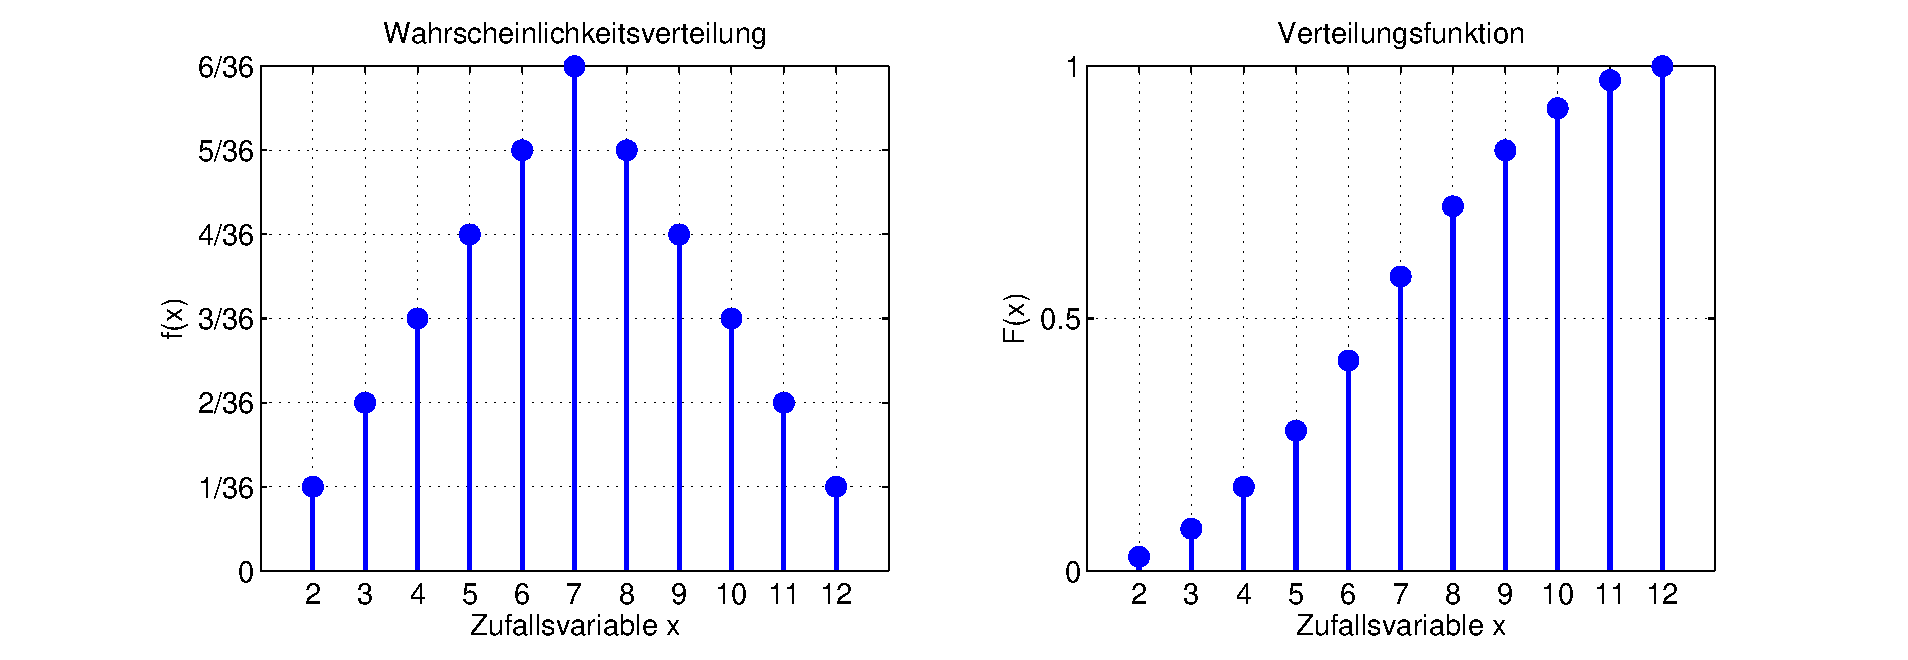
\includegraphics[width=1\textwidth]{Kapitel4/Bilder/image1}}
  \caption{Grafische Darstellung der Wahrscheinlichkeitsverteilung f(x) und Verteilungsfunktion F(x) f\"{u}r die Augenzahl beim W\"{u}rfeln mit zwei W\"{u}rfeln }
  \label{fig:Diskret_Wuerfelexperiment}
\end{figure}

\noindent Zum Beispiel ist f\"{u}r das W\"{u}rfeln die Wahrscheinlichkeit f\"{u}r einen Zahlenwert 3 $\mathrm{<}$ x $\leq$ 7 

\begin{equation}\label{eq:foursix}
P\left(3<x\le 7\right)=\sum _{x_{n} >3}^{7}f\left(x_{n} \right) =\dfrac{3}{36} +\dfrac{4}{36} +\dfrac{5}{36} +\dfrac{6}{36} =\dfrac{18}{36} =\dfrac{1}{2}
\end{equation}

\noindent Sie kann aber auch aus der Verteilungsfunktion berechnet werden. 

\begin{equation}\label{eq:fourseven}
P\left(3<x\le 7\right)=F\left(7\right)-F\left(3\right)=\dfrac{21}{36} -\dfrac{3}{36} =\dfrac{1}{2}
\end{equation}


\noindent Die Werte x$_{n}$, an denen die diskrete Zufallsvariable x eine positive Wahrscheinlichkeit besitzt, werden als m\"{o}gliche Werte von x bezeichnet. In jedem Intervall, in dem kein m\"{o}glicher Wert von x liegt, bleibt die Verteilungsfunktion F(x) konstant. F(x) ist also eine Funktion, die an den Stellen x = x$_{n}$ um die Wahrscheinlichkeit P$_{n}$ = f(x$_{n}$) springt und ansonsten konstant bleibt. F\"{u}r Werte der Zufallsvariable x, die kleiner als der kleinste m\"{o}gliche Wert x$_{min}$ sind, gilt

\begin{equation}\label{eq:foureight}
F(x<x_{\min })=0
\end{equation}

\noindent F\"{u}r den gr\"{o}{\ss}ten vorkommenden Wert x${}_{max}$ nimmt die Verteilungsfunktion den Wert 

\begin{equation}\label{eq:fournine}
F(x\ge x_{\max })=1
\end{equation}

\noindent an. Der Informationsgehalt der Wahrscheinlichkeitsverteilung f(x) und der Verteilungsfunktion F(x) sind identisch. Nach Gleichung \eqref{eq:fourfive} gilt f\"{u}r zwei Zufallsvariablen mit dem Abstand d 

\begin{equation}\label{eq:fourten}
F\left(x\right)=\sum _{x_{n} =-\infty }^{x}f\left(x_{n} \right)
\end{equation}

\noindent und

\begin{equation}\label{eq:foureleven}
F(x-d)=\sum _{x_{n} =-\infty }^{x-d}f(x_{n})
\end{equation}

\noindent Damit kann die Wahrscheinlichkeitsverteilung f(x) bestimmt werden aus der Differenz

\begin{equation}\label{eq:fourtwelve}
f\left(x\right)=F\left(x\right)-F\left(x-d\right)
\end{equation}

\noindent Die Darstellungen k\"{o}nnen also mithilfe dieser Gleichungen ineinander \"{u}berf\"{u}hrt werden. Obwohl beide Funktionen denselben Informationsgehalt haben, ist die Wahrscheinlichkeitsverteilung f(x) f\"{u}r diskrete Verteilungen die anschaulichere Darstellung. Im Gegensatz dazu muss bei Rechnungen mit stetigen Verteilungen die Verteilungsfunktion F(x) verwendet werden, weshalb beide Formen der Darstellung ihre Berechtigung haben.\newline

\noindent Die Wahrscheinlichkeitsverteilung f(x) und die Verteilungsfunktion F(x) sind vergleichbar mit den Darstellungen zur relativen H\"{a}ufigkeit h(x) und der relativen Summenh\"{a}ufigkeit H(x) in der beschreibenden Statistik. Allerdings liegt bei der beschreibenden Statistik eine konkrete Stichprobe vor, w\"{a}hrend die Wahrscheinlichkeitsverteilung f(x) und die Verteilungsfunktion F(x) die Grundgesamtheit eines Wahrscheinlichkeitsexperimentes charakterisieren. 


\subsubsection{Stetige Zufallsvariablen und Verteilungen}

\noindent Eine Zufallsvariable x ist stetig, wenn die zugeh\"{o}rige Verteilungsfunktion F(x) in Integralform dargestellt werden kann.

\begin{equation}\label{eq:fourthirteen}
P(\xi \le x)=F(x)=\int _{-\infty }^{x}f(\xi)d\xi
\end{equation}

\noindent Da in Gleichung \eqref{eq:fourthirteen}die obere Grenze des Integrals der Wert x ist, wird die Integrationsvariable mit dem griechischen $\xi$ bezeichnet. Der Integrand ist eine positive Funktion, die stetig ist oder einzelne Spr\"{u}nge aufweist. Dadurch ist die Verteilungsfunktion F(x) stetig. Der Integrand f(x) hei{\ss}t Wahrscheinlichkeitsdichte der Zufallsvariable x. Aus Gleichung \eqref{eq:fourthirteen}folgt durch Differentiation

\begin{equation}\label{eq:fourfourteen}
f(x)=\dfrac{dF}{dx}
\end{equation}

\noindent Die Wahrscheinlichkeitsdichte f(x) ist demnach die Ableitung der Verteilungsfunktion F(x). Auch bei stetigen Verteilungen ist der Informationsgehalt identisch, sie lassen sich mit den Gleichungen \eqref{eq:fourthirteen} und \eqref{eq:fourfourteen} ineinander umrechnen. Da das Ereignis - $\infty$ $\mathrm{<}$ x $\leq$ $\infty$ ein sicheres Ereignis ist, ergibt sich

\begin{equation}\label{eq:fourfifteen}
P\left(-\infty <x\le \infty \right)=F(\infty)=\int\limits _{-\infty }^{\infty }f(x)dx =1
\end{equation}

\noindent Weiterhin gilt f\"{u}r das Ereignis a $\mathrm{<}$ x $\leq$ b analog zur Gleichung \eqref{eq:fourfour}

\begin{equation}\label{eq:foursixteen}
P\left(a<x\le b\right)=F(b)-F(a)=\int\limits _{a}^{b}f(x)dx
\end{equation}

\noindent Die Wahrscheinlichkeit des Ereignisses a $\mathrm{<}$ x $\leq$ b entspricht der Fl\"{a}che unter der Kurve der Wahrscheinlichkeitsdichte f(x) zwischen den Punkten x = a und x = b. Bild \ref{fig:WahrscheinlichkeitVariableIntervall} stellt diesen Zusammenhang grafisch dar. 

\noindent 
\begin{figure}[H]
  \centerline{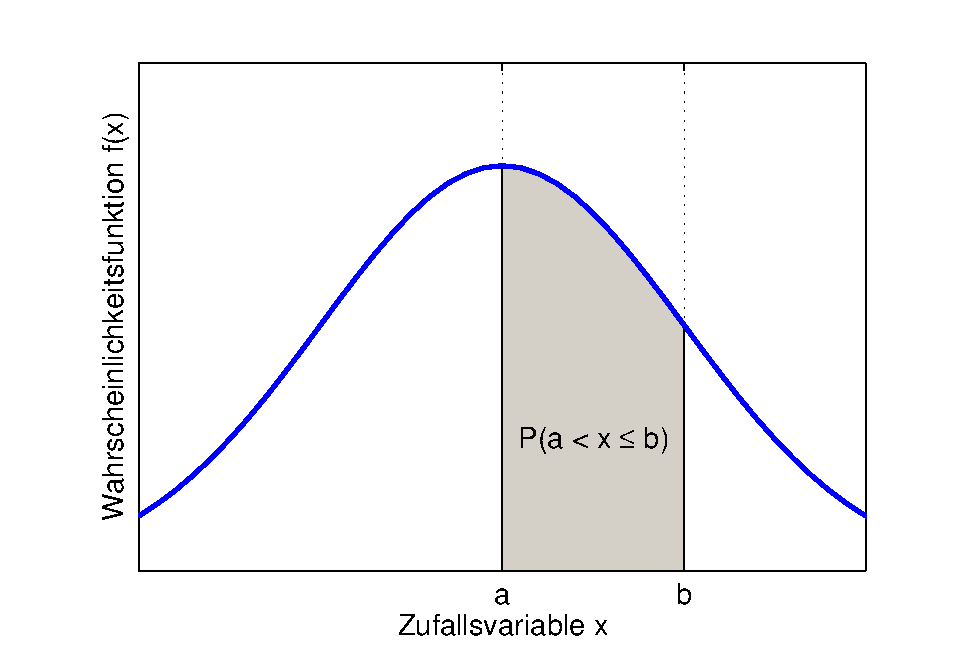
\includegraphics[width=0.5\textwidth]{Kapitel4/Bilder/image2}}
  \caption{Grafische Darstellung der Wahrscheinlichkeit P(a $\mathrm{<}$ x $\mathrm{\le}$ b)}
  \label{fig:WahrscheinlichkeitVariableIntervall}
\end{figure}

\clearpage 

\noindent F\"{u}r ein singul\"{a}res Ereignis x = a ist die Abszisse unendlich klein. Damit wird auch die Fl\"{a}che unter der Kurve unendlich klein und die Wahrscheinlichkeit f\"{u}r den Wert x = a ist 

\begin{equation}\label{eq:fourseventeen}
P(x=a)=0
\end{equation}

\noindent Das bedeutet nicht, dass x = a ein unm\"{o}gliches Ergebnis ist, sondern dass die Wahrscheinlichkeit unendlich klein ist, bei einer stetigen Zufallsvariablen genau einen definierten Wert zu erzielen.\bigskip

\noindent
\colorbox{lightgray}{%
\arrayrulecolor{white}%
\renewcommand\arraystretch{0.6}%
\begin{tabular}{ wl{16.5cm} }
{\fontfamily{phv}\selectfont{Beispiel: Gl\"{u}cksrad}}
\end{tabular}%
}\medskip 

\noindent Ein Gl\"{u}cksrad, das einen beliebigen Winkel x zwischen 0 und 2$.\pi$ einnehmen kann, kann als Zufallsexperiment aufgefasst werden. Alle Winkel x sind gleich wahrscheinlich, deshalb ist die Wahrscheinlichkeitsdichte f(x) konstant P${}_{0}$. Das sichere Ereignis ist, dass der Winkel x in dem Intervall 0 $\mathrm{<}$ x $\leq$ 2$.\pi$ liegt. Es gilt:

\begin{equation}\label{eq:foureighteen}
F(2\cdot \pi )=\int\limits _{0}^{2\cdot \pi }f(x)dx =\int\limits _{0}^{2\cdot \pi }f_{0} dx =2\cdot \pi \cdot f_{0} =1
\end{equation}

\noindent Daraus ergibt sich durch Aufl\"{o}sen nach P$_{0}$ f$_{0}$ die Wahrscheinlichkeitsdichte in dem Bereich 0 $\mathrm{<}$ x $\leq$ 2$.\pi$ von

\begin{equation}\label{eq:fournineteen}
f(x)=f_{0} =\dfrac{1}{2\cdot \pi} 
\end{equation}

\noindent und die Verteilungsfunktion

\begin{equation}\label{eq:fourtwenty}
F(x)=\int\limits _{0}^{x}\dfrac{1}{2\cdot \pi } d\xi  =\dfrac{x}{2\cdot \pi}
\end{equation}

\noindent Bild \ref{fig:Gleichverteilung} stellt die Wahrscheinlichkeitsdichte f(x) und die Verteilungsfunktion F(x) f\"{u}r das Experiment dar.

\noindent 
\begin{figure}[H]
  \centerline{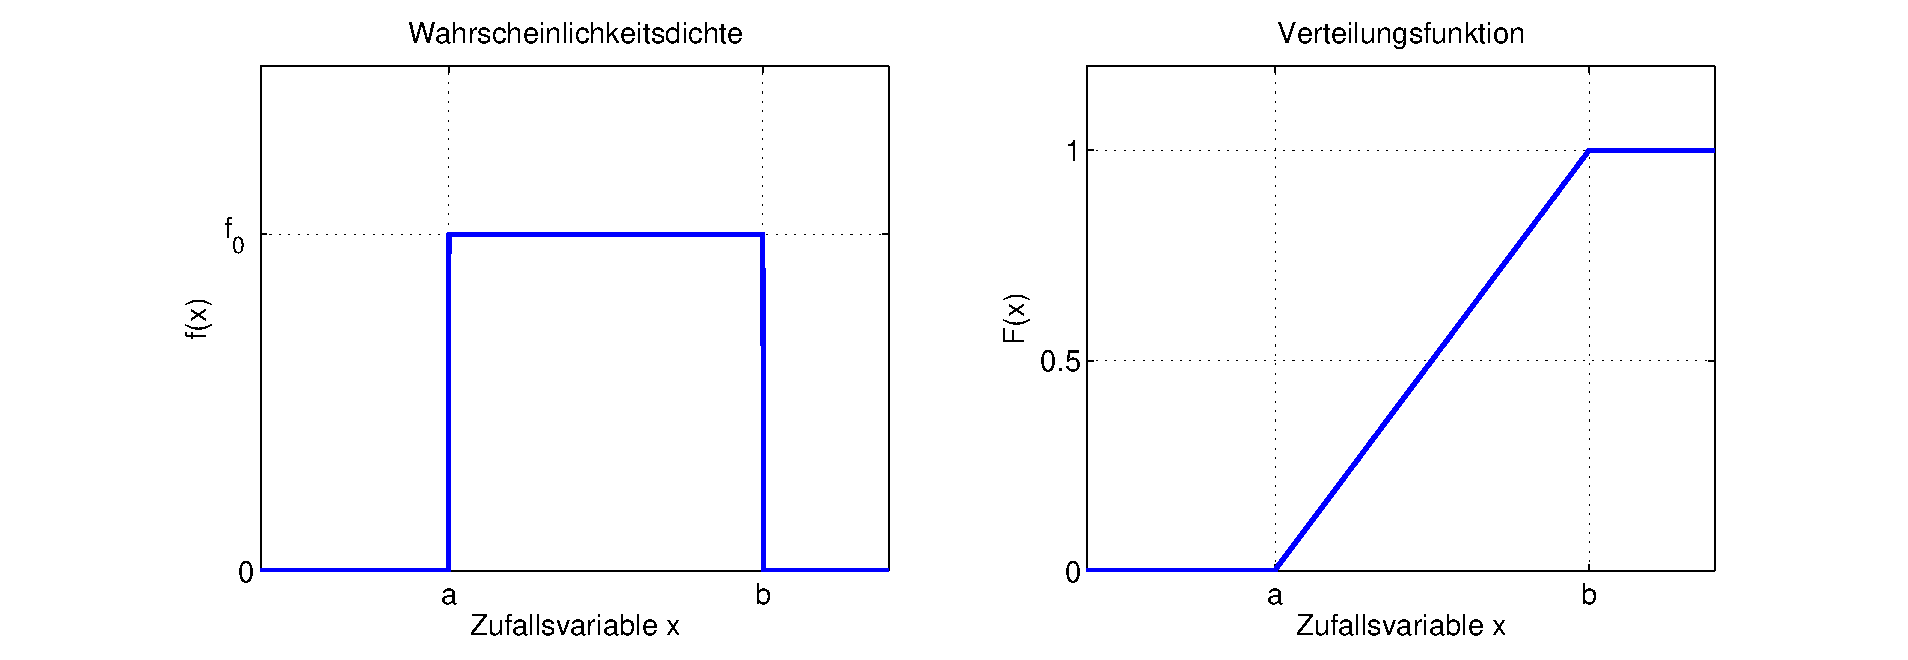
\includegraphics[width=1\textwidth]{Kapitel4/Bilder/image3}}
  \caption{Grafische Darstellung der Wahrscheinlichkeitsdichte f(x) und Verteilungsfunktion F(x) f\"{u}r das Gl\"{u}cksrad-Experiment}
  \label{fig:Gleichverteilung}
\end{figure}

\clearpage

\noindent Die Wahrscheinlichkeit, dass das Gl\"{u}cksrad mit einem Winkel in dem Bereich von a $\mathrm{<}$ x $\leq$ b stehen bleibt, ist 

\begin{equation}\label{eq:fourtwentyone}
P\left(a<x\le b\right)=\int\limits _{a}^{b}\dfrac{1}{2\cdot \pi } dx= \dfrac{b-a}{2\cdot \pi}
\end{equation}

\noindent Alle Ereignisse in dem definierten Intervall zwischen a und b sind gleich wahrscheinlich.

\subsubsection{Nomenklatur f\"{u}r diskrete und stetige Zufallsvariablen}

\noindent Diskrete und stetige Verteilungen werden mit den Funktionen f(x) und F(x) beschrieben. Die Funktion F(x) wird in beiden F\"{a}llen als Verteilungsfunktion bezeichnet. Bei diskreten Zufallsvariablen ist f(x) die Wahrscheinlichkeitsverteilung, bei stetigen Zufallsvariablen ist f(x) die Wahrscheinlichkeitsdichte. Bei Stichproben wird von relativen H\"{a}ufigkeitsverteilungen h(x) und relativen Summenh\"{a}ufigkeiten H(x) gesprochen. Damit ergeben sich die in Tabelle \ref{tab:fourthree} zusammengefassten Bezeichnungen.

\begin{table}[H]
\setlength{\arrayrulewidth}{.1em}
\caption{ Zusammenfassung der Nomenklatur f\"{u}r Stichproben sowie diskrete und stetige Zufallsvariablen}
\setlength{\fboxsep}{0pt}%
\colorbox{lightgray}{%
\arrayrulecolor{white}%
\begin{tabular}{| c | c | c |}
\hline
\parbox[c][0.3in][c]{1.9in}{\smallskip\centering\textbf{\fontfamily{phv}\selectfont{Stichprobe}}} &
\parbox[c][0.3in][c]{2.2in}{\smallskip\centering\textbf{\fontfamily{phv}\selectfont{Diskreter Zufallsprozess}}} &
\parbox[c][0.3in][c]{2.2in}{\smallskip\centering\textbf{\fontfamily{phv}\selectfont{Stetiger Zufallsprozess}}}\\ \hline

\parbox[c][0.5in][c]{1.9in}{\centering\fontfamily{phv}\selectfont{Relative Häufigkeitsverteilung h(x)}} & 
\parbox[c][0.5in][c]{2.2in}{\centering\fontfamily{phv}\selectfont{Wahrscheinlichkeitsverteilung f(x)}} &
\parbox[c][0.5in][c]{2.2in}{\centering\fontfamily{phv}\selectfont{Wahrscheinlichkeitsdichte f(x)}}\\
\hline

\parbox[c][0.5in][c]{1.9in}{\centering\fontfamily{phv}\selectfont{Relative Summenhäufigkeit H(x)}} & 
\parbox[c][0.5in][c]{2.2in}{\centering\fontfamily{phv}\selectfont{Verteilungsfunktion F(x)}} &
\parbox[c][0.5in][c]{2.2in}{\centering\fontfamily{phv}\selectfont{Verteilungsfunktion F(x)}}\\
\hline

\end{tabular}%
}
\label{tab:fourthree}
\end{table}
\noindent 

\clearpage

\subsection{Erwartungswerte von Verteilungen}

\noindent Der Erwartungswert E(x) der Zufallsvariablen x entspricht dem Wert, der sich bei oftmaligem Wiederholen des zugrunde liegenden Zufallsexperiments im Mittel einstellt. Durch den Erwartungswert E(x) wird sp\"{a}ter die Lage der vorliegenden Verteilung beschrieben. Der Erwartungswert kann aber nicht nur von der Zufallsvariablen x bestimmt werden, sondern auch von Funktionen von Zufallsvariablen g(x). Der Erwartungswert eignet sich damit zur Bestimmung von Kenngr\"{o}{\ss}en einer Verteilung. Dieser Zusammenhang wird in Abschnitten \ref{fourthree} gezeigt.


\subsubsection{Definition des Erwartungswert-Operators}

\noindent F\"{u}r eine beliebige Zufallsvariable x und eine f\"{u}r alle Werte von x definierte reellwertige Funktion y = g(x) der Zufallsvariablen x wird der Ausdruck 

\begin{equation}\label{eq:fourtwentytwo}
E(y)=E\left(g(x)\right)=\sum _{x_{n} =-\infty }^{\infty }\left(g(x_{n})\cdot f(x_{n})\right)
\end{equation}

\noindent beziehungsweise 

\begin{equation}\label{eq:fourtwentythree}
E(y)=E\left(g(x)\right)=\int\limits _{-\infty}^{\infty}g(x)\cdot f(x)dx
\end{equation}

\noindent als mathematischer Erwartungswert der Funktion g(x) oder als Erwartung von g(x) bezeichnet. Dabei wird die Konvergenz der Summe beziehungsweise des Integrals vorausgesetzt.\bigskip

\noindent
\colorbox{lightgray}{%
\arrayrulecolor{white}%
\renewcommand\arraystretch{0.6}%
\begin{tabular}{ wl{16.5cm} }
{\fontfamily{phv}\selectfont{Beispiel:Gl\"{u}cksspiel mit W\"{u}rfeln}}
\end{tabular}%
}\medskip 

\noindent Zwei Personen A und B spielen das folgende Spiel: A w\"{u}rfelt mit einem regelm\"{a}{\ss}igen W\"{u}rfel und erh\"{a}lt von B

\begin{itemize}
    \item 10 Cent f\"{u}r eine Eins oder Zwei,
    \item 20 Cent f\"{u}r eine Drei oder Vier,
    \item 40 Cent f\"{u}r eine F\"{u}nf und
    \item 80 Cent f\"{u}r eine Sechs.
\end{itemize}

\noindent Spieler A soll an Spieler B vor jedem Spiel einen Betrag von 50 Cent zahlen. Um zu \"{u}berpr\"{u}fen, ob Spieler A bei mehreren Spielen einen Gewinn erzielt, muss die durchschnittliche Gewinnerwartung pro Spiel berechnet werden. Die durchschnittliche Gewinnerwartung ergibt sich aus der Wahrscheinlichkeit, eine bestimmte Zahl zu w\"{u}rfeln, und dem zugeordneten Gewinn. Zum Beispiel betr\"{a}gt die Wahrscheinlichkeit, eine Eins zu w\"{u}rfeln, 1/6, und der zugeh\"{o}rige Gewinn betr\"{a}gt 10 Cent. 

\noindent Zur Berechnung wird eine Zufallsvariable x definiert, die die beim Wurf des W\"{u}rfels erzielte Augenzahl darstellt. In Tabelle \ref{tab:fourfour} ist jedem m\"{o}glichen Wert der Zufallsvariablen x der Gewinn von A zugeordnet. Er bildet die Funktion g(x).

\begin{table}[H]
\setlength{\arrayrulewidth}{.1em}
\caption{Zuordnung des Gewinns g(x) zur Zufallsvariablen x}
\setlength{\fboxsep}{0pt}%
\colorbox{lightgray}{%
\arrayrulecolor{white}%
\begin{tabular}{| wc{2cm} | wc{2cm} | wc{2cm} | wc{2cm} | wc{2cm} | wc{2cm} | wc{2cm} }
\hline\xrowht{15pt}

\fontfamily{phv}\selectfont{x} & 1 & 2 & 3 & 4 & 5 & 6 \\ \hline \xrowht{25pt}

\fontfamily{phv}\selectfont{(x)} & 10 & 10 & 20 & 20 & 40 & 80\\ \hline

\end{tabular}%
}
\label{tab:fourfour}
\end{table}

\noindent Da die Werte von x vom Zufall abh\"{a}ngen, gilt dies auch f\"{u}r den Wert, den g(x) bei einem Spiel jeweils annimmt. Die Funktion g(x) der Zufallsvariable x ist also selbst eine Zufallsvariable y = g(x). In diesem Beispiel betr\"{a}gt die durchschnittliche Gewinnerwartung

\begin{equation}\label{eq:fourtwentyfour}
E(y)=E(g(x))=\sum _{x_{n} =1}^{6}\left(g(x_{n})\cdot f(x_{n})\right) =10\cdot \dfrac{1}{6} +10\cdot \dfrac{1}{6} +20\cdot \dfrac{1}{6} +20\cdot \dfrac{1}{6} +40\cdot \dfrac{1}{6} +80\cdot \dfrac{1}{6} =30
\end{equation}

\noindent Die durchschnittliche Gewinnerwartung pro Spiel ist mit 30 Cent geringer als der Spieleinsatz von 50 Cent. Spieler A wird bei mehreren Spieldurchg\"{a}ngen demnach Geld verlieren.

\subsubsection{Eigenschaften des Erwartungswert-Operators}

\noindent Es gibt einige Eigenschaften des Erwartungswert-Operators, die dazu verwendet werden k\"{o}nnen, den Erwartungswert von Funktionen von Zufallsvariablen zu bestimmen. Da der Erwartungswert f\"{u}r stetige Zufallsgr\"{o}{\ss}en \"{u}ber ein Integral definiert ist, ergeben sich die Eigenschaften des Erwartungswert-Operators aus den Eigenschaften der Integralrechnung. Im Folgenden werden Rechenregeln f\"{u}r den Erwartungswert stetiger Zufallsvariablen hergeleitet. Dieselben Rechenregeln gelten auch f\"{u}r diskrete Zufallsvariablen.\bigskip

{\fontfamily{phv}\selectfont
\noindent\textbf{Erwartungswert einer Konstanten}}\smallskip

\noindent Der Erwartungswert einer konstanten Gr\"{o}{\ss}e k besitzt den Wert k, denn es gilt:

\begin{equation}\label{eq:fourtwentyfive}
E(k)=\int\limits _{-\infty }^{\infty }k \cdot f(x)dx=k\cdot \int\limits _{-\infty }^{\infty }f(x) dx =k\cdot 1=k
\end{equation}

{\fontfamily{phv}\selectfont
\noindent\textbf{Linearit\"{a}t des Erwartungswert-Operators}}\smallskip

\noindent Der Erwartungswert ist ein linearer Operator. F\"{u}r die Zufallsvariable 

\begin{equation}\label{eq:fourtwentysix}
y=a\cdot h(x)+b\cdot g(x)
\end{equation}

\noindent wird der Erwartungswert berechnet aus

\begin{equation}\label{eq:fourtwentyseven}
\begin{split}
E(y) & = E\left(a\cdot h(x)+b\cdot g(x)\right)=\int\limits _{-\infty }^{\infty }(a\cdot h(x)+b\cdot g(x)) \cdot f(x)dx \\
& = a\cdot \int\limits _{-\infty }^{\infty }h(x) \cdot f(x)dx+b\cdot \int\limits _{-\infty }^{\infty }g(x) \cdot f(x)dx=a\cdot E(h(x))+b\cdot E(g(x))  
\end{split}
\end{equation}

\noindent Ein Sonderfall ist die lineare Transformation der Form 

\begin{equation}\label{eq:fourtwentyeight}
y=a\cdot x+b
\end{equation}

\noindent Aufgrund der Linearit\"{a}t des Erwartungswertes ergibt sich 

\begin{equation}\label{eq:fourtwentynine}
E(y)=E(a\cdot x+b)=a\cdot E(x)+b
\end{equation}

\noindent Ein Vergleich der Gleichungen \eqref{eq:fourtwentyeight} und \eqref{eq:fourtwentynine} zeigt, dass sich der Erwartungswert analog zur Zufallsvariable verschiebt. \bigskip

{\fontfamily{phv}\selectfont
\noindent\textbf{Erwartungswert symmetrischer Verteilungen}}\smallskip

\noindent F\"{u}r Ist eine zum Punkt c symmetrische Verteilung f(x) symmetrisch zum Punkt c

\begin{equation}\label{eq:fourthirty}
f(c-x)=f(c+x)
\end{equation}

\noindent gilt f\"{u}r den soll der Erwartungswert-Operator

\begin{equation}\label{eq:fourthirtyone}
E(x)=\int\limits _{-\infty }^{\infty }x\cdot f(x)dx =\int\limits _{-\infty }^{c}x\cdot f(x)dx +\int\limits _{c}^{\infty }x\cdot f(x)dx
\end{equation}

\noindent berechnet werden. Durch die Substitution x = c - $\xi$ beziehungsweise x = c + $\xi$ ergibt sich

\begin{equation}\label{eq:fourthirtytwo}
E(x)=\int\limits _{0}^{\infty }(c-\xi )\cdot f(c-\xi )d\xi  +\int\limits _{0}^{\infty }(c+\xi )\cdot f(c+\xi )d\xi
\end{equation}

\noindent Wegen der identischen Integrationsgrenzen k\"{o}nnen die Integrale zusammengefasst werden.

\begin{equation}\label{eq:fourthirtythree}
\begin{split}
E(x) & = \int\limits _{0}^{\infty }c\cdot f(c-\xi)d\xi  +\int\limits _{0}^{\infty }c\cdot f(c+\xi)d\xi  -\int\limits _{0}^{\infty }\xi \cdot f(c-\xi )d\xi  +\int\limits _{0}^{\infty }\xi \cdot f(c+\xi)d\xi\\
& =  \int\limits _{-\infty}^{\infty }c\cdot f(c-\xi)d\xi - \int\limits _{0}^{\infty }\xi\cdot (f(c-\xi)  -  f(c+\xi ))d\xi
\end{split}
\end{equation}

\noindent Der erste Summand ist der Erwartungswert einer konstanten Gr\"{o}{\ss}e c. Der zweite Summand besteht aus einer Differenz von Wahrscheinlichkeitsdichten. Da die Wahrscheinlichkeitsdichte symmetrisch ist, ist die Differenz null. Damit ergibt sich der Erwartungswert einer symmetrischen Verteilung zu

\begin{equation}\label{eq:fourthirtyfour}
E(x)=c\cdot \int\limits _{-\infty }^{\infty }f\left(c-\xi \right) d\xi  -0=c
\end{equation}

\clearpage

{\fontfamily{phv}\selectfont
\noindent\textbf{Zusammenfassung}}\smallskip

\noindent In Tabelle \ref{tab:fourfive} werden die Eigenschaften des Erwartungswert-Operators zusammengefasst. Das Rechnen mit Erwartungswerten ist insbesondere bei der Herleitung von Gesetzm\"{a}{\ss}igkeiten f\"{u}r die Grundgesamtheit und die Berechnung der Erwartungstreue bei Sch\"{a}tzungen von Bedeutung.

\begin{table}[H]
\setlength{\arrayrulewidth}{.1em}
\caption{Zusammenfassung der Eigenschaften des Erwartungswert-Operators}
\setlength{\fboxsep}{0pt}%
\colorbox{lightgray}{%
\arrayrulecolor{white}%
\begin{tabular}{| c | c |}
\hline
\parbox[c][0.35in][c]{2.5in}{\smallskip\centering\textbf{\fontfamily{phv}\selectfont{Rechenoperation}}} & \parbox[c][0.35in][c]{4.2in}{\smallskip\centering\textbf{\fontfamily{phv}\selectfont{Eigenschaften des Erwartungswert-Operators}}}\\ \hline

\parbox[c][1.6in][c]{2.5in}{\centering\fontfamily{phv}\selectfont{Definition Erwartungswert}} & 
\parbox[c][1.6in][c]{4.2in}{\centering\fontfamily{phv}\selectfont{$E\left(y\right)=E(g(x))=\sum _{x_{n} =-\infty }^{\infty }\left(g(x_{n} )\cdot f(x_{n} )\right) $\bigskip

beziehungsweise\bigskip

$E(y)=E(g(x))=\int\limits _{-\infty }^{\infty }g(x)\cdot f(x)dx$}}\\ \hline

\parbox[c][0.4in][c]{2.5in}{\centering{\fontfamily{phv}\selectfont{Erwartungswert einer Konstanten}}} & 
\parbox[c][0.4in][c]{4.2in}{\centering{$E\left(k\right)=k$}}\\ \hline

\parbox[c][0.4in][c]{2.5in}{\centering{\fontfamily{phv}\selectfont{Linearität}}} & 
\parbox[c][0.4in][c]{4.2in}{\centering{$E(a\cdot h(x)+b\cdot g(x))=a\cdot E(h(x))+b\cdot E(g(x))$}}\\ \hline

\parbox[c][0.4in][c]{2.5in}{\centering{\fontfamily{phv}\selectfont{Lineare Transformation}}} & 
\parbox[c][0.4in][c]{4.2in}{\centering{$E(y)=E(a\cdot x+b)=a\cdot E(x)+b$}}\\ \hline

\parbox[c][0.4in][c]{2.5in}{\centering{\fontfamily{phv}\selectfont{Symmetrie f(c -- x) = f(x -- c)}}} & 
\parbox[c][0.4in][c]{4.2in}{\centering{$E(x)=c$}}\\ \hline

\end{tabular}%
}
\label{tab:fourfive}
\end{table}

\clearpage

\subsection{Kennwerte von Verteilungen}

\noindent Bei der beschreibenden Statistik werden vorliegende Daten aus Stichproben analysiert. Dabei werden f\"{u}r die konkreten Daten H\"{a}ufigkeitsverteilungen bestimmt sowie empirische Kenngr\"{o}{\ss}en f\"{u}r die Lage, die Streuung und die Symmetrie berechnet. Diese Kenngr\"{o}{\ss}en lassen sich auch f\"{u}r Verteilungen Zufallsvariablen mit einer bekannten Wahrscheinlichkeitsverteilung berechnen. Im Gegensatz zur deskriptiven Statistik werden bei der Wahrscheinlichkeitsrechnung alle theoretisch m\"{o}glichen Werte der Zufallsvariablen ausgewertet. Deshalb werden die Kennwerte auch als theoretische Kennwerte bezeichnet.

\subsubsection{Momente und Zentralmomente einer Verteilung}

\noindent Kennwerte von Verteilungen k\"{o}nnen als Moment beziehungsweise als Zentralmoment der Ordnung k berechnet werden. Das k-te Moment einer Verteilung oder der Zufallsvariable x ist definiert als der Erwartungswert der Funktion 

\begin{equation}\label{eq:fourthirtyfive}
g(x)=x^{k}
\end{equation}

\noindent F\"{u}r diskrete Verteilungen ergibt sich 

\begin{equation}\label{eq:fourthirtysix}
E(x^{k})=\sum _{x_{n} =-\infty }^{\infty }\left(x_{n}^{k} \cdot f(x_{n})\right)
\end{equation}

\noindent und f\"{u}r stetige Verteilungen berechnet sich das k-te Moment zu

\begin{equation}\label{eq:fourthirtyseven}
E(x^{k})=\int\limits _{-\infty }^{\infty }x^{k} \cdot f(x) dx
\end{equation}

\noindent Der Erwartungswert der Funktion 

\begin{equation}\label{eq:fourthirtyeight}
g(x)=(x-\mu)^{k}
\end{equation}

\noindent f\"{u}hrt zu dem k-ten Zentralmoment. Dabei ist µ der arithmetische Mittelwert der Verteilung, auf ihn wird in Abschnitt 4.3.2 detailliert eingegangen. F\"{u}r diskrete Verteilungen berechnet sich das k-te Zentralmoment aus 

\begin{equation}\label{eq:fourthirtynine}
E\left((x-\mu)^{k} \right)=\sum _{x_{n} =-\infty }^{\infty }\left((x_{n} -\mu)^{k} \cdot f(x_{n} )\right)
\end{equation}

\noindent und f\"{u}r stetige Verteilungen aus

\begin{equation}\label{eq:fourfourty}
E\left((x-\mu)^{k} \right)=\int\limits _{-\infty }^{\infty }\left(x-\mu \right)^{k} \cdot f(x)dx
\end{equation}

\noindent Aufgrund der Linearit\"{a}t des Erwartungswertes kann die Berechnung des Zentralmomentes auf die Berechnung des Momentes zur\"{u}ckgef\"{u}hrt werden. Zum Beispiel ergibt sich f\"{u}r das zweite Zentralmoment 

\begin{equation}\label{eq:fourfourtyone}
\begin{split}
E\left(\left(x-\mu \right)^{2} \right) & = E\left(x^{2} -2\cdot \mu \cdot x+\mu ^{2} \right)=E\left(x^{2} \right)-2\cdot \mu \cdot E\left(x\right)+\mu ^{2}\\
& = E(x^{2}) -2\cdot\mu ^{2} +\mu ^{2} = E(x^{2})-\mu ^{2}
\end{split}
\end{equation}

\noindent Entsprechend k\"{o}nnen h\"{o}here Zentralmomente umgeformt werden. F\"{u}r das dritte Zentralmoment ergibt sich mit den Rechenregeln des Erwartungswertes 

\begin{equation}\label{eq:fourfourtytwo}
E\left((x-\mu )^{3} \right)=E(x^{3} )-3\cdot \mu \cdot E(x^{2})+2\cdot \mu ^{3}
\end{equation}

\subsubsection{Lagekennwerte einer Verteilung}

\noindent Wie bei der deskriptiven Statistik k\"{o}nnen f\"{u}r Wahrscheinlichkeitsverteilungen Lagekennwerte angegeben werden. In Anlehnung an die beschreibende Statistik werden in diesem Abschnitt der arithmetische Mittelwert und der Median einer Verteilung eingef\"{u}hrt.

{\fontfamily{phv}\selectfont
\noindent\textbf{Arithmetischer Mittelwert einer Verteilung}}\smallskip

\noindent Der theoretisch erwartete Mittelwert einer Verteilung wird mit µ bezeichnet. Er berechnet sich bei einer diskreten Verteilung zu

\begin{equation}\label{eq:fourfourtythree}
\mu =\sum _{x_{n} =-\infty }^{\infty }\left(x_{n} \cdot f\left(x_{n} \right)\right)
\end{equation}

\noindent und bei einer stetigen Verteilung zu

\begin{equation}\label{eq:fourfourtyfour}
\mu =\int\limits _{-\infty }^{\infty }x\cdot f(x)dx
\end{equation}

\noindent Der Mittelwert kann auch als Erwartungswert eines Momentes erster Ordnung dargestellt werden. 

\begin{equation}\label{eq:fourfourtyfive}
\mu =E(x^{1})=E(x)
\end{equation}

\noindent Der Mittelwert der Verteilung wird auch als Mittelwert der Zufallsvariable x oder Erwartungswert von x bezeichnet. Bei der Berechnung des Mittelwertes wird vorausgesetzt, dass die Summe \eqref{eq:fourfourtythree} beziehungsweise das Integral \eqref{eq:fourfourtyfour} konvergieren, was aber in praktischen F\"{a}llen immer gegeben ist.\bigskip

{\fontfamily{phv}\selectfont
\noindent\textbf{Median einer Verteilung}}\smallskip

\noindent Der Median einer Verteilung ergibt sich aus der Bedingung

\begin{equation}\label{eq:fourfourtysix}
F\left(x_{MED} \right)=0.5
\end{equation}

\noindent Im Fall einer stetigen Zufallsvariable x ist in praktischen F\"{a}llen auch die Verteilungsfunktion F(x) stetig. Damit kann der Median analytisch oder zumindest numerisch bestimmt werden. Im Fall einer diskreten Zufallsvariable x muss der Median mit vergleichbaren Verfahren wie bei der deskriptiven Statistik bestimmt werden.

\clearpage

\noindent
\colorbox{lightgray}{%
\arrayrulecolor{white}%
\renewcommand\arraystretch{0.6}%
\begin{tabular}{ wl{16.5cm} }
{\fontfamily{phv}\selectfont{Beispiel: W\"{u}rfeln mit zwei W\"{u}rfeln}}
\end{tabular}%
}\medskip  

\noindent Bei dem Beispiel des W\"{u}rfelns mit zwei W\"{u}rfeln ergibt sich ein Mittelwert von 

\begin{equation}\label{eq:fourfourtyseven}
\mu =\sum _{x_{n} =-\infty }^{\infty }\left(x_{n} \cdot f(x_{n} )\right) =7
\end{equation}

\noindent Der Median errechnet sich nach den Darstellungen zur deskriptiven Statistik aus

\begin{equation}\label{eq:fourfourtyeight}
x_{MED} =c_{n-1} +\dfrac{0.5-F(c_{n-1})}{f(c_{n})} \cdot d=6+\dfrac{0.5-\dfrac{15}{36} }{\dfrac{6}{36} } \cdot 1=6+\dfrac{1}{2} =6.5
\end{equation}

\noindent
\colorbox{lightgray}{%
\arrayrulecolor{white}%
\renewcommand\arraystretch{0.6}%
\begin{tabular}{ wl{16.5cm} }
{\fontfamily{phv}\selectfont{Beispiel: Gl\"{u}cksrad}}
\end{tabular}%
}\medskip 

\noindent Bei dem Beispiel des Gl\"{u}cksrades ergibt sich ein Mittelwert von

\begin{equation}\label{eq:fourfourtynine}
\mu =\int\limits _{0}^{2\cdot \pi }x\cdot f\left(x\right)dx =\int\limits _{0}^{2\cdot \pi}x\cdot \dfrac{1}{2\cdot \pi} dx =\left. \dfrac{1}{2\cdot \pi } \cdot (\dfrac{x^{2}}{2})\right|_{0}^{2\cdot \pi} =\pi
\end{equation}

\noindent Der Median ergibt sich aus Bild \ref{fig:Gleichverteilung} zu

\begin{equation}\label{eq:fourfifty}
x_{MED} =\pi
\end{equation}

\subsubsection{Streuungskennwerte einer Verteilung}

\noindent Analog zu den Lagekennwerten von Verteilungen k\"{o}nnen Streuungskennwerte angegeben werden. In diesem Abschnitt werden die Spannweite, die Varianz und die Quantile einer Verteilung eingef\"{u}hrt.\bigskip

{\fontfamily{phv}\selectfont
\noindent\textbf{Spannweite einer Verteilung}}\smallskip

\noindent Sind die Ereignisse der Verteilung f(x) auf ein Intervall I begrenzt, kann die Spannweite der Verteilung angegeben werden als 

\begin{equation}\label{eq:fourfiftyone}
\Delta x=\max (I)-\min (I)
\end{equation}

{\fontfamily{phv}\selectfont
\noindent\textbf{Varianz und Standardabweichung einer Verteilung}}\smallskip

\noindent Die Varianz einer Verteilung ist ein Ma{\ss} f\"{u}r die theoretisch erwartete Streuung der Werte, die die Zufallsvariable x annehmen kann. Sie wird mit $\sigma^{2}$ bezeichnet und ist \"{u}ber den Erwartungswert des zweiten Zentralmomentes 

\begin{equation}\label{eq:fourfiftytwo}
\sigma ^{2} =E\left((x-\mu)^{2} \right)
\end{equation}

\noindent definiert. Im diskreten Fall berechnet sie sich zu

\begin{equation}\label{eq:fourfiftythree}
\sigma ^{2} =\sum _{x_{n} =-\infty }^{\infty }\left((x_{n} -\mu)^{2} \cdot f(x_{n})\right)
\end{equation}

\noindent und im stetigen Fall zu

\begin{equation}\label{eq:fourfiftyfour}
\sigma ^{2} =\int\limits _{-\infty }^{\infty }\left(x-\mu \right)^{2} \cdot f(x)dx
\end{equation}

\noindent Die Varianz einer Verteilung wird auch als Varianz der Zufallsvariable x bezeichnet. Die Varianz der Verteilung kann mit den Rechenregeln des Erwartungswertes umgeformt werden zu

\begin{equation}\label{eq:fourfiftyfive}
\sigma ^{2} =E\left((x-\mu)^{2} \right)=E\left(x^{2} -2\cdot x\cdot \mu +\mu ^{2} \right)=E(x^{2})-2\cdot \mu \cdot E(x)+\mu ^{2} =E(x^{2})-\mu ^{2}
\end{equation}

\noindent Aus den Definitionsgleichungen ergibt sich, dass die Varianz immer gr\"{o}{\ss}er oder gleich 0 ist. Die positive Wurzel der Varianz wird bei der beschreibenden Statistik als Standardabweichung eingef\"{u}hrt. F\"{u}r diskrete Verteilungen berechnet sich die Standardabweichung $\sigma$ aus 

\begin{equation}\label{eq:fourfiftysix}
\sigma =\sqrt{\sum _{x_{n} =-\infty }^{\infty }\left((x_{n} -\mu)^{2} \cdot f(x_{n})\right)}
\end{equation}

\noindent und f\"{u}r stetige Verteilungen ergibt sich 

\begin{equation}\label{eq:fourfiftyseven}
\sigma =\sqrt{\int\limits _{-\infty }^{\infty }\left(x-\mu \right)^{2} \cdot f(x) dx}
\end{equation}

{\fontfamily{phv}\selectfont
\noindent\textbf{Quantilabst\"{a}nde einer Verteilung}}\smallskip

\noindent Analog zum Median einer Verteilung ergibt sich aus der Bedingung

\begin{equation}\label{eq:fourfiftyeight}
F(x_{P})=P
\end{equation}

\noindent das P-Quantil einer Verteilung. Im Fall einer stetigen Zufallsvariable x ist auch die Verteilungsfunktion F(x) stetig. Damit kann das P-Quantil analytisch oder zumindest numerisch bestimmt werden. Im Fall einer diskreten Zufallsvariable muss das P-Quantil wieder mit vergleichbaren Verfahren bestimmt werden, wie bei der deskriptiven Statistik. Der Quantilabstand berechnet sich dann aus der Differenz zweier Quantile. Der Inter-Quartil-Range berechnet sich zu

\begin{equation}\label{eq:fourfiftynine}
IQR=x_{0.75} -x_{0.25}
\end{equation}

\noindent
\colorbox{lightgray}{%
\arrayrulecolor{white}%
\renewcommand\arraystretch{0.6}%
\begin{tabular}{ wl{16.5cm} }
{\fontfamily{phv}\selectfont{Beispiel: W\"{u}rfeln mit zwei W\"{u}rfeln}}
\end{tabular}%
}\medskip 

\noindent Bei dem Beispiel des W\"{u}rfelns mit zwei W\"{u}rfeln ergibt sich eine Spannweite von 

\begin{equation}\label{eq:foursixty}
\Delta x=\max (I)-\min (I)=12-2=10
\end{equation}

\noindent Die Varianz von

\begin{equation}\label{eq:foursixtyone}
\sigma ^{2} =\sum _{x_{n} =-\infty }^{\infty }\left(\left(x_{n} -\mu \right)^{2} \cdot f(x_{n} )\right) =5.83
\end{equation}

\noindent f\"{u}hrt zu einer Standardabweichung

\begin{equation}\label{eq:foursixtytwo}
\sigma =\sqrt{\sum _{x_{n} =-\infty }^{\infty }\left((x_{n} -\mu)^{2} \cdot f(x_{n})\right) } =\sqrt{5.83} =2.41
\end{equation}

\noindent Der Inter-Quartil-Range errechnet sich zu

\begin{equation}\label{eq:foursixtythree}
IQR=x_{0.75} -x_{0.25} =8.25-4.75=3.5
\end{equation}

\noindent
\colorbox{lightgray}{%
\arrayrulecolor{white}%
\renewcommand\arraystretch{0.6}%
\begin{tabular}{ wl{16.5cm} }
{\fontfamily{phv}\selectfont{Beispiel: Gl\"{u}cksrad}}
\end{tabular}%
}\medskip 

\noindent Bei dem Gl\"{u}cksrad erstreckt sich das Intervall I von 0 bis 2$.\pi$, die Spannweite betr\"{a}gt damit $\Delta$x = 2$.\pi$. Die Varianz betr\"{a}gt

\begin{equation}\label{eq:foursixtyfour}
\sigma ^{2} =\int\limits _{-\infty }^{\infty }(x-\mu)^{2} \cdot f(x)dx =\int\limits _{0}^{2\cdot \pi}(x-\pi)^{2} \cdot \dfrac{1}{2\cdot \pi} dx =\dfrac{1}{3} \cdot \pi ^{2}
\end{equation}

\noindent Damit ergibt sich eine Standardabweichung von 

\begin{equation}\label{eq:foursixtyfive}
\sigma =\sqrt{\int\limits _{-\infty}^{\infty}\left(x-\mu \right)^{2} \cdot f(x)dx} =\sqrt{\int\limits _{0}^{2\cdot \pi}(x-\pi)^{2} \cdot \dfrac{1}{2\cdot \pi} dx} =\dfrac{1}{\sqrt{3}} \cdot \pi
\end{equation}

\noindent Aus Bild \ref{fig:Gleichverteilung} kann der Inter-Quartil-Range bestimmt werden zu

\begin{equation}\label{eq:foursixtysix}
IQR=x_{0.75} -x_{0.25} =\dfrac{3\cdot \pi}{2} -\dfrac{\pi}{2} =\pi
\end{equation}

\subsubsection{Schiefe oder Symmetrie einer Verteilung}

\noindent Nachdem die Begriffe des Momentes und Zentralmomentes einer Verteilung eingef\"{u}hrt sind, wird die Symmetrie einer Verteilung mit dem Momenten- und Quantilkoeffizienten der Schiefe beschrieben. 

{\fontfamily{phv}\selectfont
\noindent\textbf{Momentenkoeffizient der Schiefe}}\smallskip

\noindent Analog zum Momentenkoeffizient der Schiefe in der deskriptiven Statistik wird das dritte normierte zentrale Moment zur Definition der Schiefe $\gamma$ einer Verteilung verwendet: 

\begin{equation}\label{eq:foursixtyseven}
\gamma =\dfrac{1}{\sigma ^{3}} \cdot E\left((x-\mu)^{3} \right)
\end{equation}

{\fontfamily{phv}\selectfont
\noindent\textbf{Quantilkoeffizient der Schiefe}}\smallskip

\noindent Alternativ kann die Symmetrie oder Schiefe einer Verteilung \"{u}ber eine Kenngr\"{o}{\ss}e charakterisiert werden, die die Symmetrie der Quantile der Verteilung bewertet. Dazu wird der Quantilkoeffizient der Schiefe wie bei der deskriptiven Statistik berechnet aus

\begin{equation}\label{eq:foursixtyeight}
g_{P} =\dfrac{(x_{1-P} -x_{MED})-\left(x_{MED} -x_{P} \right)}{x_{1-P} -x_{P}}
\end{equation}

\noindent F\"{u}r P = 25 \% ergibt sich der Quartilkoeffizient zu

\begin{equation}\label{eq:foursixtynine}
g_{0.25} =\dfrac{\left(x_{0.75} -x_{MED} \right)-\left(x_{MED} -x_{0.25} \right)}{x_{0.75} -x_{0.25} }
\end{equation}

\noindent Die Interpretation des Momenten- oder Quantilkoeffizienten der Schiefe erfolgt analog zu den Ausf\"{u}hrungen bei der deskriptiven Statistik.

\begin{table}[H]
\setlength{\arrayrulewidth}{.1em}
\caption{Bewertung des Momentenkoeffizienten der Schiefe}
\setlength{\fboxsep}{0pt}%
\colorbox{lightgray}{%
\arrayrulecolor{white}%
\begin{tabular}{| c | c |}
\hline
\parbox[c][0.3in][c]{3.3in}{\smallskip\centering\textbf{\fontfamily{phv}\selectfont{Kennwert}}} & 
\parbox[c][0.3in][c]{3.3in}{\smallskip\centering\textbf{\fontfamily{phv}\selectfont{Symmetrieeigenschaft}}}\\ \hline


\parbox[c][0.3in][c]{3.3in}{\centering\fontfamily{phv}\selectfont{$g_{P} \mathrm{>} 0$}} & 
\parbox[c][0.3in][c]{3.3in}{\centering\fontfamily{phv}\selectfont{Rechtsschiefe Verteilung}} \\
\hline

\parbox[c][0.3in][c]{3.3in}{\centering\fontfamily{phv}\selectfont{$g_{P}= 0$}} & 
\parbox[c][0.3in][c]{3.3in}{\centering\fontfamily{phv}\selectfont{Symmetrische Verteilung}} \\
\hline

\parbox[c][0.3in][c]{3.3in}{\centering\fontfamily{phv}\selectfont{$g_{P} \mathrm{<} 0$}} & 
\parbox[c][0.3in][c]{3.3in}{\centering\fontfamily{phv}\selectfont{Linksschiefe Verteilung}} \\
\hline

\end{tabular}%
}
\label{tab:foursix}
\end{table}

\noindent
\colorbox{lightgray}{%
\arrayrulecolor{white}%
\renewcommand\arraystretch{0.6}%
\begin{tabular}{ wl{16.5cm} }
{\fontfamily{phv}\selectfont{Beispiel: Schiefe einer Verteilung}}
\end{tabular}%
}\medskip 

\noindent Die Schiefe einer stetigen Verteilung wird an einem Beispiel verdeutlicht.

\begin{equation}\label{eq:fourseventy}
f(x)=\left\{\begin{array}{ll}
{0 \qquad \;\;\; \text{ für } x<0} \\
{x\cdot e^{-x}  \quad \text{für} x\ge 0} \end{array}\right.
\end{equation}

\noindent Bild \ref{fig:SchiefeVerteilung} stellt die Verteilung aus Gleichung \eqref{eq:fourseventy} dar.

\begin{figure}[H]
  \centerline{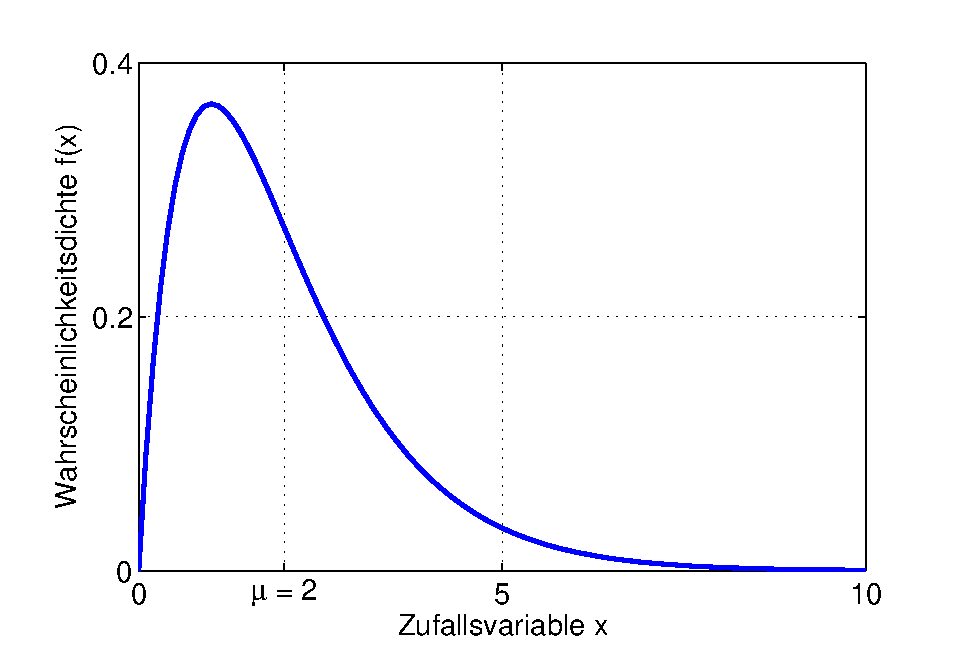
\includegraphics[width=0.5\textwidth]{Kapitel4/Bilder/image4}}
  \caption{Grafische Darstellung der Wahrscheinlichkeitsverteilung aus Gleichung \eqref{eq:fourseventy}}
  \label{fig:SchiefeVerteilung}
\end{figure}

\clearpage

\noindent Durch Einsetzen in die Definitionsgleichungen ergibt sich der Mittelwert zu

\begin{equation}\label{eq:fourseventyone}
\mu =E(x)=\int _{0}^{\infty}{x}^{2} \cdot {e}^{-x}dx=2
\end{equation}

\noindent das zweite Moment zu

\begin{equation}\label{eq:fourseventytwo}
E(x^{2})=\int _{0}^{\infty}{x}^{3} \cdot {e}^{-x} dx =6
\end{equation}

\noindent und das dritte Moment zu

\begin{equation}\label{eq:fourseventythree}
E(x^{3})=\int _{0}^{\infty }{x}^{4} \cdot {e}^{-x} dx =24
\end{equation}

\noindent Mit den Gleichungen \eqref{eq:fourfiftyfive} und \eqref{eq:foursixtyseven} sowie \eqref{eq:fourseventytwo} und \eqref{eq:fourseventythree} k\"{o}nnen die Varianz und die Schiefe der Verteilung berechnet werden zu 

\begin{equation}\label{eq:fourseventyfour}
\sigma ^{2} =E\left((x-\mu)^{2} \right)=E(x^{2})-\mu ^{2} =6-4=2
\end{equation}

\begin{equation}\label{eq:fourseventyfive}
\gamma =\dfrac{1}{\sigma ^{3} } \cdot \left(E(x^{3})-3\cdot \mu \cdot E(x^{2})+2\cdot \mu ^{3} \right)=\dfrac{24-3\cdot 2\cdot 6+2\cdot 8}{2\cdot \sqrt{2} } =\sqrt{2}
\end{equation}

\noindent Es handelt sich um eine Funktion mit positiver Schiefe $\gamma$ = 1.4, die Verteilung ist damit rechtsschief.

\clearpage

{\fontfamily{phv}\selectfont
\noindent\textbf{Lageregeln zur Interpretation der Symmetrie einer Stichprobe}}\smallskip

\noindent Die Symmetrieeigenschaften der Verteilung einer Stichprobe k\"{o}nnen auch an der Lage von Median und Mittelwert abgelesen werden. Auch dazu wird auf die Ausf\"{u}hrungen zur deskriptiven Statistik verwiesen. 

\begin{table}[H]
\setlength{\arrayrulewidth}{.1em}
\caption{Lageregeln von Median und arithmetischem Mittelwert zur Beschreibung der Symmetrie}
\setlength{\fboxsep}{0pt}%
\colorbox{lightgray}{%
\arrayrulecolor{white}%
\begin{tabular}{| c | c |}
\hline
\parbox[c][0.3in][c]{3.3in}{\smallskip\centering\textbf{\fontfamily{phv}\selectfont{Lagekennwerte}}} & 
\parbox[c][0.3in][c]{3.3in}{\smallskip\centering\textbf{\fontfamily{phv}\selectfont{Symmetrieeigenschaft}}}\\ \hline


\parbox[c][0.3in][c]{3.3in}{\centering\fontfamily{phv}\selectfont{$\mu >x_{MED} $}} & 
\parbox[c][0.3in][c]{3.3in}{\centering\fontfamily{phv}\selectfont{Rechtsschiefe Verteilung}} \\
\hline

\parbox[c][0.3in][c]{3.3in}{\centering\fontfamily{phv}\selectfont{$\mu =x_{MED} $}} & 
\parbox[c][0.3in][c]{3.3in}{\centering\fontfamily{phv}\selectfont{Symmetrische Verteilung}} \\
\hline

\parbox[c][0.3in][c]{3.3in}{\centering\fontfamily{phv}\selectfont{$\mu <x_{MED} $}} & 
\parbox[c][0.3in][c]{3.3in}{\centering\fontfamily{phv}\selectfont{Linksschiefe Verteilung}} \\
\hline

\end{tabular}%
}
\label{tab:fourseven}
\end{table}

\clearpage

\subsubsection{Zusammenfassung Kennwerte von Verteilungen}

\noindent Tabelle \ref{tab:foureight} fasst die Kennwerte von Verteilungen zusammen. Die Definition der Parameter \"{u}ber Momente ist von gr\"{o}{\ss}erem praktischen Nutzen und wird in den folgenden Kapiteln weiter ben\"{o}tigt und ausgebaut.

\begin{table}[H]
\setlength{\arrayrulewidth}{.1em}
\caption{Zusammenfassung der Kennwerte von Verteilungen}
\setlength{\fboxsep}{0pt}%
\colorbox{lightgray}{%
\arrayrulecolor{white}%
\begin{tabular}{| wc{5.5cm} | wc{5.5cm} | wc{5.5cm} }
\hline\xrowht{20pt}

\multirow{2}{*}{\fontfamily{phv}\selectfont\textbf{Momente}} & \multicolumn{2}{c}{\fontfamily{phv}\selectfont\textbf{Basis f\"{u}r Definition}} \\ \xrowht{15pt}
& \fontfamily{phv}\selectfont\textbf{Momente} & 
\fontfamily{phv}\selectfont\textbf{Quantile} \\ \hline \xrowht{12.5pt}

\multirow{3}{*}{\fontfamily{phv}\selectfont{Lage}} &
\fontfamily{phv}\selectfont{Mittelwert}  & 
\fontfamily{phv}\selectfont{Median} \\ \xrowht{12.5pt}
& $\mu =E(x^{1})=E(x)$ & $F(x_{MED})=0.5$ \\ \hline\xrowht{12.5pt}

\multirow{3}{*}{\fontfamily{phv}\selectfont{Streuung}} &
\fontfamily{phv}\selectfont{Varianz}  & 
\fontfamily{phv}\selectfont{Inter-Quartil-Range} \\ \xrowht{12.5pt}
& $\sigma ^{2} =E((x-\mu)^{2})$ & $IQR=x_{0.75} -x_{0.25} $ \\ \hline\xrowht{25pt}

\multirow{3}{*}{\fontfamily{phv}\selectfont{Streuung}} &
\fontfamily{phv}\selectfont{Varianz}  & 
\fontfamily{phv}\selectfont{Inter-Quartil-Range} \\ \xrowht{25pt}
& $\gamma =\dfrac{1}{\sigma ^{3} } \cdot E((x-\mu)^{3})$ & $g_{0.25} =\dfrac{(x_{0.75} -x_{0.5})-(x_{0.5} -x_{0.25})}{x_{0.75} -x_{0.25} } $ \\ \hline

\end{tabular}%
}
\label{tab:foureight}
\end{table}

\clearpage

\subsection{Funktionen von Zufallsvariablen}

\noindent Als Zufallsvariable wird allgemein eine Variable bezeichnet, die dem Ergebnis eines Zufallsexperimentes eine reelle Zahl zuordnet. Die reelle Zahl kann \"{u}ber eine Funktion 

\begin{equation}\label{eq:fourseventysix}
y=g(x)
\end{equation}

\noindent abgebildet werden. Es wird von einer Funktion der Zufallsvariable x gesprochen. Bild \ref{fig:DarstellungFunktionVonZufallsvariablen} verdeutlicht die Abbildung der Variable x auf die Variable y \"{u}ber die Funktion g(x).

\noindent 
\begin{figure}[H]
  \centerline{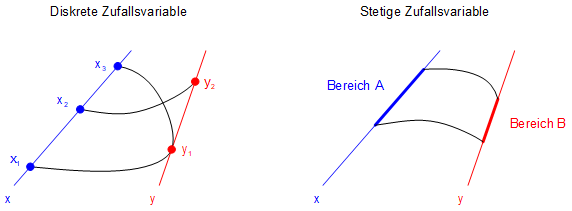
\includegraphics[width=1\textwidth]{Kapitel4/Bilder/image5}}
  \caption{Grafische Veranschaulichung der Funktion von Zufallsvariable}
  \label{fig:DarstellungFunktionVonZufallsvariablen}
\end{figure}

\noindent F\"{u}r die Berechnung praktischer Aufgabenstellungen zur Variable y ist es erforderlich, die Wahrscheinlichkeitsverteilung der Variable y zu kennen. Sie kann berechnet werden, wenn die Verteilungsfunktion der Variable x bekannt ist.

\subsubsection{Funktion einer diskreten Zufallsvariable}

\noindent Bei diskreten Zufallsvariablen wird einem Zufallsereignis eine feste Zahl x$_{n}$ zugeordnet. Durch eine Abbildung

\begin{equation}\label{eq:fourseventyseven}
y_{n} =g(x_{n})
\end{equation}

\noindent ändert sich an der Wahrscheinlichkeit des zugrunde liegenden Ereignisses nichts, sodass sich die Wahrscheinlichkeit von x$_{n}$ auf y$_{n}$ \"{u}bertr\"{a}gt. Bild \ref{fig:DarstellungFunktionVonZufallsvariablen} macht deutlich, dass die Variable y$_{n}$ m\"{o}glicherweise durch unterschiedliche Variable x$_{n}$ erreicht werden kann. Damit errechnet sich die Wahrscheinlichkeit der Zufallsvariable y$_{n}$ \"{a}hnlich wie bei Ereignisb\"{a}umen aus der Summe

\begin{equation}\label{eq:fourseventyeight}
f_{Y} (y_{n})=\sum _{y_{n} =g(x_{n})}f_{X}(x_{n})
\end{equation}

\noindent Bei bekannter Wahrscheinlichkeitsverteilung f$_{Y}$(y) errechnet sich die Verteilungsfunktion der Variable y definitionsgem\"{a}{\ss} zu

\begin{equation}\label{eq:fourseventynine}
F_{Y} (y)=\sum _{y_{n} =-\infty }^{y}f_{Y} (y_{n})
\end{equation}

\clearpage 

\noindent
\colorbox{lightgray}{%
\arrayrulecolor{white}%
\renewcommand\arraystretch{0.6}%
\begin{tabular}{ wl{16.5cm} }
{\fontfamily{phv}\selectfont{Beispiel: Abbildung einer diskreten Zufallsvariable}}
\end{tabular}%
}\medskip 

\noindent Gegeben ist eine Zufallsvariable x. Ihr Ereignisraum und ihre Wahrscheinlichkeitsverteilung sind in Tabelle \ref{tab:fournine} dargestellt. Die Zufallsvariable x wird \"{u}ber die Funktion 

\begin{equation}\label{eq:foureighty}
y=(x-1)^{2}
\end{equation}

\noindent auf eine Zufallsvariable y abgebildet. Sie ist ebenfalls in Tabelle \ref{tab:fournine} aufgef\"{u}hrt.

\begin{table}[H]
\caption{Diskrete Zufallsvariable x und ihre Wahrscheinlichkeitsverteilung $f_{X}(x)$}
\setlength{\fboxsep}{0pt}%
\colorbox{lightgray}{%
\arrayrulecolor{white}%
\begin{tabular}{| c | c | c | c | c | c |}
\hline

\parbox[c][0.28in][c]{0.97in}{\smallskip\centering\textbf{\fontfamily{phv}\selectfont{$x_{n}$}}} &
\parbox[c][0.28in][c]{0.97in}{\centering{-1}} &
\parbox[c][0.28in][c]{0.97in}{\centering{0}} &
\parbox[c][0.28in][c]{0.97in}{\centering{1}} &
\parbox[c][0.28in][c]{0.97in}{\centering{2}} &
\parbox[c][0.28in][c]{0.97in}{\centering{3}} \\ \hline

\parbox[c][0.28in][c]{0.97in}{\smallskip\centering\textbf{\fontfamily{phv}\selectfont{$f_{X}(x_{n})$}}} &
\parbox[c][0.28in][c]{0.97in}{\centering{0.1}} &
\parbox[c][0.28in][c]{0.97in}{\centering{0.2}} &
\parbox[c][0.28in][c]{0.97in}{\centering{0.4}} &
\parbox[c][0.28in][c]{0.97in}{\centering{0.2}} &
\parbox[c][0.28in][c]{0.97in}{\centering{0.1}} \\ \hline

\parbox[c][0.28in][c]{0.97in}{\smallskip\centering\textbf{\fontfamily{phv}\selectfont{$y_{n}$}}} &
\parbox[c][0.28in][c]{0.97in}{\centering{4}} &
\parbox[c][0.28in][c]{0.97in}{\centering{1}} &
\parbox[c][0.28in][c]{0.97in}{\centering{0}} &
\parbox[c][0.28in][c]{0.97in}{\centering{1}} &
\parbox[c][0.28in][c]{0.97in}{\centering{4}} \\ \hline

\end{tabular}%
}\bigskip
\label{tab:fournine}
\end{table}

\noindent Da zum Beispiel der Wert y = 1 \"{u}ber x = 0 und x = 2 erreicht werden kann, werden die entsprechenden Wahrscheinlichkeiten f\"{u}r das Ereignis y = 1 addiert.

\begin{equation}\label{eq:foureightyone}
f_{Y} (y=1)=f_{X}(x=0)+f_{X} (x=2)=0.2+0.2=0.4
\end{equation}

\noindent Es ergibt sich die in Tabelle \ref{tab:fourten} gezeigte Wahrscheinlichkeitsverteilung und Verteilungsfunktion der Zufallsvariable y.

\begin{table}[H]
\caption{Diskrete Zufallsvariable y und ihre Wahrscheinlichkeitsverteilung $f_{Y}(y)$}
\setlength{\fboxsep}{0pt}%
\colorbox{lightgray}{%
\arrayrulecolor{white}%
\begin{tabular}{| c | c | c | c |}
\hline

\parbox[c][0.28in][c]{1.54in}{\smallskip\centering\textbf{\fontfamily{phv}\selectfont{$y_{n}$}}} &
\parbox[c][0.28in][c]{1.54in}{\centering{0}} &
\parbox[c][0.28in][c]{1.54in}{\centering{1}} &
\parbox[c][0.28in][c]{1.54in}{\centering{4}} \\ \hline

\parbox[c][0.28in][c]{1.54in}{\smallskip\centering\textbf{\fontfamily{phv}\selectfont{$f_{Y}(y_{n})$}}} &
\parbox[c][0.28in][c]{1.54in}{\centering{0.4}} &
\parbox[c][0.28in][c]{1.54in}{\centering{0.4}} &
\parbox[c][0.28in][c]{1.54in}{\centering{0.2}}  \\ \hline

\parbox[c][0.28in][c]{1.54in}{\smallskip\centering\textbf{\fontfamily{phv}\selectfont{$F_{Y}(y_{n})$}}} &
\parbox[c][0.28in][c]{1.54in}{\centering{0.4}} &
\parbox[c][0.28in][c]{1.54in}{\centering{0.8}} &
\parbox[c][0.28in][c]{1.54in}{\centering{1}}  \\ \hline

\end{tabular}%
}\bigskip
\label{tab:fourten}
\end{table}

\subsubsection{Funktion einer kontinuierlichen Zufallsvariable}

\noindent Auch bei kontinuierlichen Zufallsvariablen wird einem Zufallsereignis eine Zahl x zugeordnet. Durch die Abbildung

\begin{equation}\label{eq:foureightytwo}
y=g(x)
\end{equation}

\noindent entsteht eine Zufallsvariable y, deren Verteilungsfunktion F$_{Y}$(y) im Folgenden f\"{u}r streng monoton steigende Funktionen g(x) hergeleitet wird. Die Verteilungsfunktion F$_{Y}$(y) ist definiert als die Wahrscheinlichkeit, dass eine Variable $\psi$ kleiner als der Wert y ist. Da die Zufallsvariable $\psi$ = g($\xi$) definiert ist, gilt

\begin{equation}\label{eq:foureightythree}
yF_{Y} (y)=P\left(\psi \le y\right)=P\left(g(\xi)\le y\right)
\end{equation}

\clearpage

\noindent Die Funktion g(x) ist streng monoton steigend. Damit gilt:

\begin{equation}\label{eq:foureightyfour}
F_{Y} (y)=P\left(\xi \le g^{-1} (y)\right)=F_{X} (g^{-1}(y))
\end{equation}

\noindent Aus der Verteilungsfunktion F$_{Y}$(y) errechnet sich die Wahrscheinlichkeitsdichte f$_{Y}$(y) mit der Kettenregel der Differentiationsrechnung zu

\begin{equation}\label{eq:foureightyfive}
f_{Y} (y)=\dfrac{dF_{Y}}{dy} =\dfrac{dF_{X} (g^{-1} (y))}{dg^{-1} (y)} \cdot \dfrac{dg^{-1} (y)}{dy} =f_{X} (g^{-1} (y))\cdot \dfrac{dg^{-1} (y)}{dy}
\end{equation}

\noindent Die Regel kann auf Funktionen g(x) verallgemeinert werden, die streng monoton sind. Es ergibt sich

\begin{equation}\label{eq:foureightysix}
f_{Y} (y)=\dfrac{dF_{Y} }{dy} =\dfrac{dF_{X} \left(g^{-1} (y)\right)}{dg^{-1} (y)} \cdot \dfrac{dg^{-1} \left(y\right)}{dy} =f_{X} (g^{-1} (y))\cdot \left|\dfrac{dg^{-1} (y)}{dy} \right|
\end{equation}

\noindent
\colorbox{lightgray}{%
\arrayrulecolor{white}%
\renewcommand\arraystretch{0.6}%
\begin{tabular}{ wl{16.5cm} }
{\fontfamily{phv}\selectfont{Beispiel: Abbildung einer kontinuierlichen Zufallsvariable}}
\end{tabular}%
}\medskip 

\noindent Gegeben ist eine Zufallsvariable x, die in dem Bereich 0 $\mathrm{<}$ x $\leq$ 2 eine Wahrscheinlichkeitsdichte 

\begin{equation}\label{eq:foureightyseven}
f_{X} (x)=\dfrac{1}{2} \cdot x
\end{equation}

\noindent und Verteilungsfunktion

\begin{equation}\label{eq:foureightyeight}
F_{X} \left(x\right)=\dfrac{1}{4} \cdot x^{2}
\end{equation}

\noindent aufweist. Beide Funktionen sind in Bild \ref{fig:FunktionVonZufallsvariablen1} dargestellt.

\noindent 
\begin{figure}[H]
  \centerline{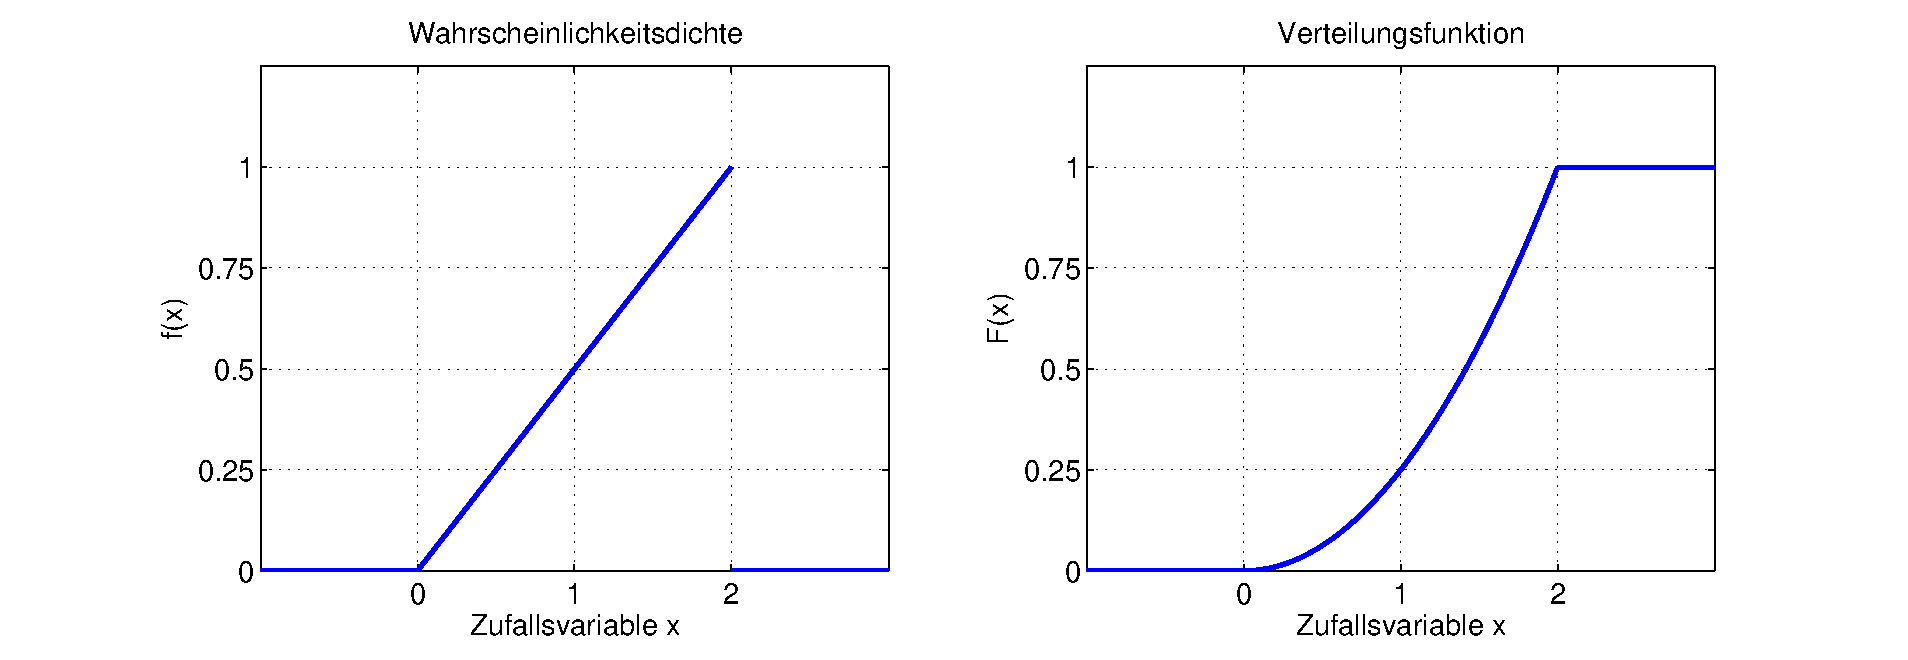
\includegraphics[width=1\textwidth]{Kapitel4/Bilder/image6}}
  \caption{Wahrscheinlichkeitsdichte f$_{X}$(x) und Verteilungsfunktion F$_{X}$(x) der kontinuierlichen Zufallsvariable x}
  \label{fig:FunktionVonZufallsvariablen1}
\end{figure}

\clearpage

\noindent Die Zufallsvariable x wird mit der Funktion 

\begin{equation}\label{eq:foureightynine}
y=g(x)=\dfrac{1}{2} \cdot x^{2}
\end{equation}

\noindent auf die Zufallsvariable y abgebildet. In dem Bereich von 0 $\mathrm{<}$ x $\leq$ 2 lautet die Umkehrfunktion

\begin{equation}\label{eq:fourninety}
x=g^{-1} (y)=\sqrt{2\cdot y}
\end{equation}

\noindent Die Verteilungsfunktion der Variable y errechnet sich zu

\begin{equation}\label{eq:fourninetyone}
F_{Y} (y)=F_{X} \left(g^{-1} (y)\right)=\left. \dfrac{1}{4} \cdot x^{2} \right|_{x=\sqrt{2\cdot y}} =\dfrac{1}{4} \cdot 2\cdot y=\dfrac{1}{2} \cdot y
\end{equation}

\noindent In dem relevanten Bereich von 0 $\mathrm{<}$ x $\leq$ 2 ist die Funktion g(x) streng monoton steigend. Damit ergibt sich die Wahrscheinlichkeitsdichte

\begin{equation}\label{eq:fourninetytwo}
f_{Y} (y)=f_{X} \left(g^{-1} (y)\right)\cdot \left|\dfrac{dg^{-1} (y)}{dy} \right|=\left. \dfrac{1}{2} \cdot x\right|_{x=\sqrt{2\cdot u}} \cdot \dfrac{d}{du} \sqrt{2\cdot u} =\dfrac{1}{2} \cdot \sqrt{2\cdot u} \cdot \sqrt{2} \cdot \dfrac{1}{2} \cdot \dfrac{1}{\sqrt{u}} =\dfrac{1}{2}
\end{equation}

\noindent Wahrscheinlichkeitsdichte und Verteilungsfunktion der Zufallsvariable y sind in Bild \ref{fig:FunktionVonZufallsvariablen2} dargestellt.

\noindent 
\begin{figure}[H]
  \centerline{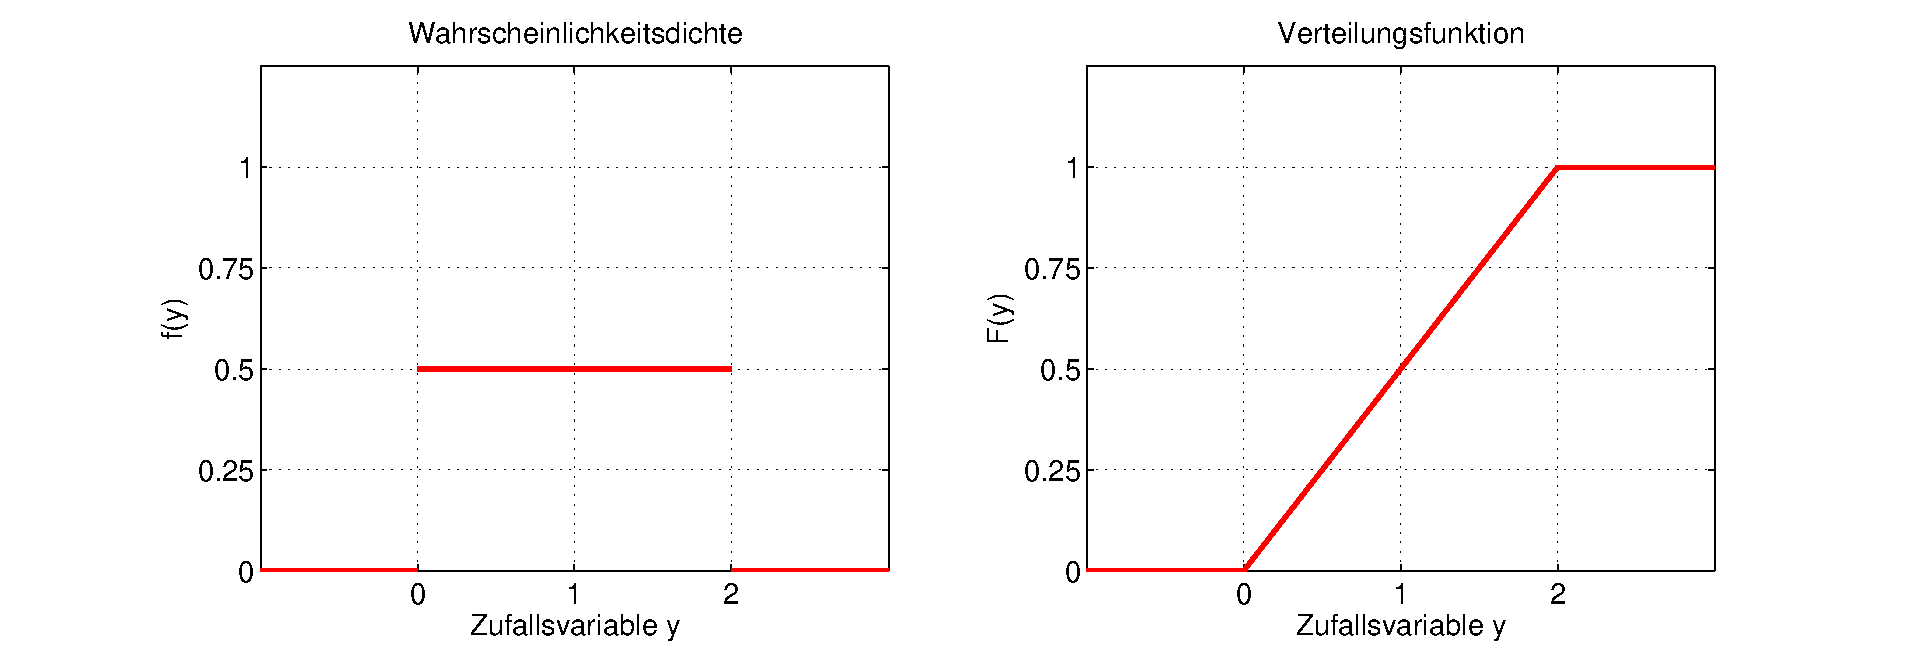
\includegraphics[width=1\textwidth]{Kapitel4/Bilder/image7}}
  \caption{Wahrscheinlichkeitsdichte f$_{Y}$(y) und Verteilungsfunktion F$_{Y}$(y) der kontinuierlichen Zufallsvariable y}
  \label{fig:FunktionVonZufallsvariablen2}
\end{figure}

\noindent Die Abbildung von Zufallsvariablen hat zwei wichtige Anwendungen: die Standardisierung von Zufallsvariablen und die numerische Generierung von Zufallsvariablen mit einer definierten Verteilung.


\subsubsection{Lineare Abbildung und Standardisierung einer Zufallsvariable}\label{fourthree}

\noindent Eine Zufallsvariable y ist über die lineare Abbildung 

\begin{equation}\label{eq:fourninetythree}
y=a\cdot x+b
\end{equation}

\noindent mit a $\mathrm{>}$ 0 definiert. Ihre Wahrscheinlichkeitsdichte errechnet sich nach Gleichung \eqref{eq:foureightysix} zu

\begin{equation}\label{eq:fourninetyfour}
f_{Y} (y)=f_{X} \left(\dfrac{y-b}{a} \right)\cdot \left|\dfrac{1}{a} \right|
\end{equation}

\noindent Die Zufallsvariable y besitzt einen Mittelwert von

\begin{equation}\label{eq:fourninetyfive}
\mu _{y} =E(y)=E\left(a\cdot x+b\right)=a\cdot E(x)+b=a\cdot \mu _{x} +b
\end{equation}

\noindent und eine Varianz von

\begin{equation}\label{eq:fourninetysix}
\begin{split}
\sigma _{y}^{2} & = E\left((y-\mu _{y})^{2} \right)=E\left(y^{2} \right)-E(y)^{2} =E\left((a\cdot x+b)^{2} \right)-E(a\cdot x+b)^{2}\\
& = E\left( a^{2}\cdot x^{2} + 2\cdot a\cdot b\cdot x + b^{2} \right) - \left(E(a\cdot x)^{2} + 2\cdot E(a\cdot x)\cdot E(b)+E(b)^{2} \right )\\
& = a^{2}\cdot E\left(x^{2}\right )+2\cdot a \cdot b\cdot E(x)+b^{2}-a^{2}\cdot E(x)^{2}-2\cdot a\cdot b\cdot E(x) -b^{2}\\
& = a^{2}\cdot \left(E(x^{2})-E(x)^{2}\right ) = a^{2} \cdot \sigma _{x}^{2}
\end{split}
\end{equation}

\noindent Die Standardabweichung der Zufallsvariablen y ergibt sich aus der positiven Wurzel der Varianz zu

\begin{equation}\label{eq:fourninetyseven}
\sigma _{y} =\sqrt{\sigma _{y}^{2}} =\sqrt{a^{2} \cdot \sigma _{x}^{2}} =a\cdot \sigma _{x}
\end{equation}

\noindent Ein Sonderfall der linearen Abbildung ist die Standardisierung von Zufallsvariablen. Standardisierte Zufallsvariablen weisen einen Mittelwert von $\mu_{y}$ = 0 und eine Standardabweichung von $\sigma_{y}$ = 1 auf. Aus diesen beiden Bedingungen ergeben sich zwei Gleichungen f\"{u}r die beiden unbekannten Variablen a und b:

\begin{equation}\label{eq:fourninetyeight}
\mu _{y} =a\cdot \mu _{x} +b=0
\end{equation}

\begin{equation}\label{eq:fourninetynine}
\sigma _{y}^{2} =a^{2} \cdot \sigma _{x}^{2} =1
\end{equation}

\noindent Aus den Bedingungen f\"{u}r a und b 

\begin{equation}\label{eq:fourhundred}
a=\dfrac{1}{\sigma _{x}}
\end{equation}

\noindent und 

\begin{equation}\label{eq:fourhundredone}
b=-\dfrac{\mu _{x} }{\sigma _{x}}
\end{equation}

\noindent ergibt sich die standardisierte Zufallsvariable

\begin{equation}\label{eq:fourhundredtwo}
y=a\cdot x+b=\dfrac{x}{\sigma _{x} } -\dfrac{\mu _{x}}{\sigma _{x}} =\dfrac{x-\mu _{x}}{\sigma _{x}}
\end{equation}

\noindent Standardisierte Zufallsvariablen sind mittelwertfrei und weisen eine Varianz von 1 auf. Sie sind insbesondere im Zusammenhang von Testverteilungen von Bedeutung.\bigskip

\noindent
\colorbox{lightgray}{%
\arrayrulecolor{white}%
\renewcommand\arraystretch{0.6}%
\begin{tabular}{ wl{16.5cm} }
{\fontfamily{phv}\selectfont{Beispiel: Gl\"{u}cksrad}}
\end{tabular}%
}\medskip 

\noindent Die Standardisierung von Zufallsvariablen wird an dem Beispiel des Gl\"{u}cksrads vertieft. Mit dem Mittelwert 

\begin{equation}\label{eq:fourhundredthree}
\mu _{x} =\pi 
\end{equation}

\noindent und der Standardabweichung von 

\begin{equation}\label{eq:fourhundredfour}
\sigma _{x} =\dfrac{1}{\sqrt{3}} \cdot \pi
\end{equation}

\noindent ergibt sich die Abbildungsgleichung zu

\begin{equation}\label{eq:fourhundredfive}
y=\dfrac{x-\mu _{x}}{\sigma _{x}} =\dfrac{x-\pi}{\dfrac{1}{\sqrt{3}} \cdot \pi } =\sqrt{3} \cdot \dfrac{x-\pi}{\pi}
\end{equation}

\noindent Durch die Transformation werden die Intervallgrenzen von 0 und 2$\pi$ abgebildet auf

\begin{equation}\label{eq:fourhundredsix}
y_{\min } =\sqrt{3} \cdot \dfrac{0-\pi}{\pi} =-\sqrt{3}
\end{equation}

\noindent und 

\begin{equation}\label{eq:fourhundredseven}
y_{\max} =\sqrt{3} \cdot \dfrac{2\cdot \pi -\pi}{\pi} =\sqrt{3}
\end{equation}

\noindent Die Wahrscheinlichkeitsdichte ergibt sich in dem Zahlenbereich y$_{min}$ $\mathrm{<}$ y $\leq$ y$_{max}$ aus der Bedingung f\"{u}r das sichere Ereignis zu

\begin{equation}\label{eq:fourhundredeight}
f(y)=\dfrac{1}{2\cdot \sqrt{3}}
\end{equation}

Bild \ref{fig:Standardisierung} stellt f\"{u}r das Gl\"{u}cksrad die Verteilung der Zufallsvariable x und der standardisierten Zufallsvariable y gegen\"{u}ber.

\noindent 
\begin{figure}[H]
  \centerline{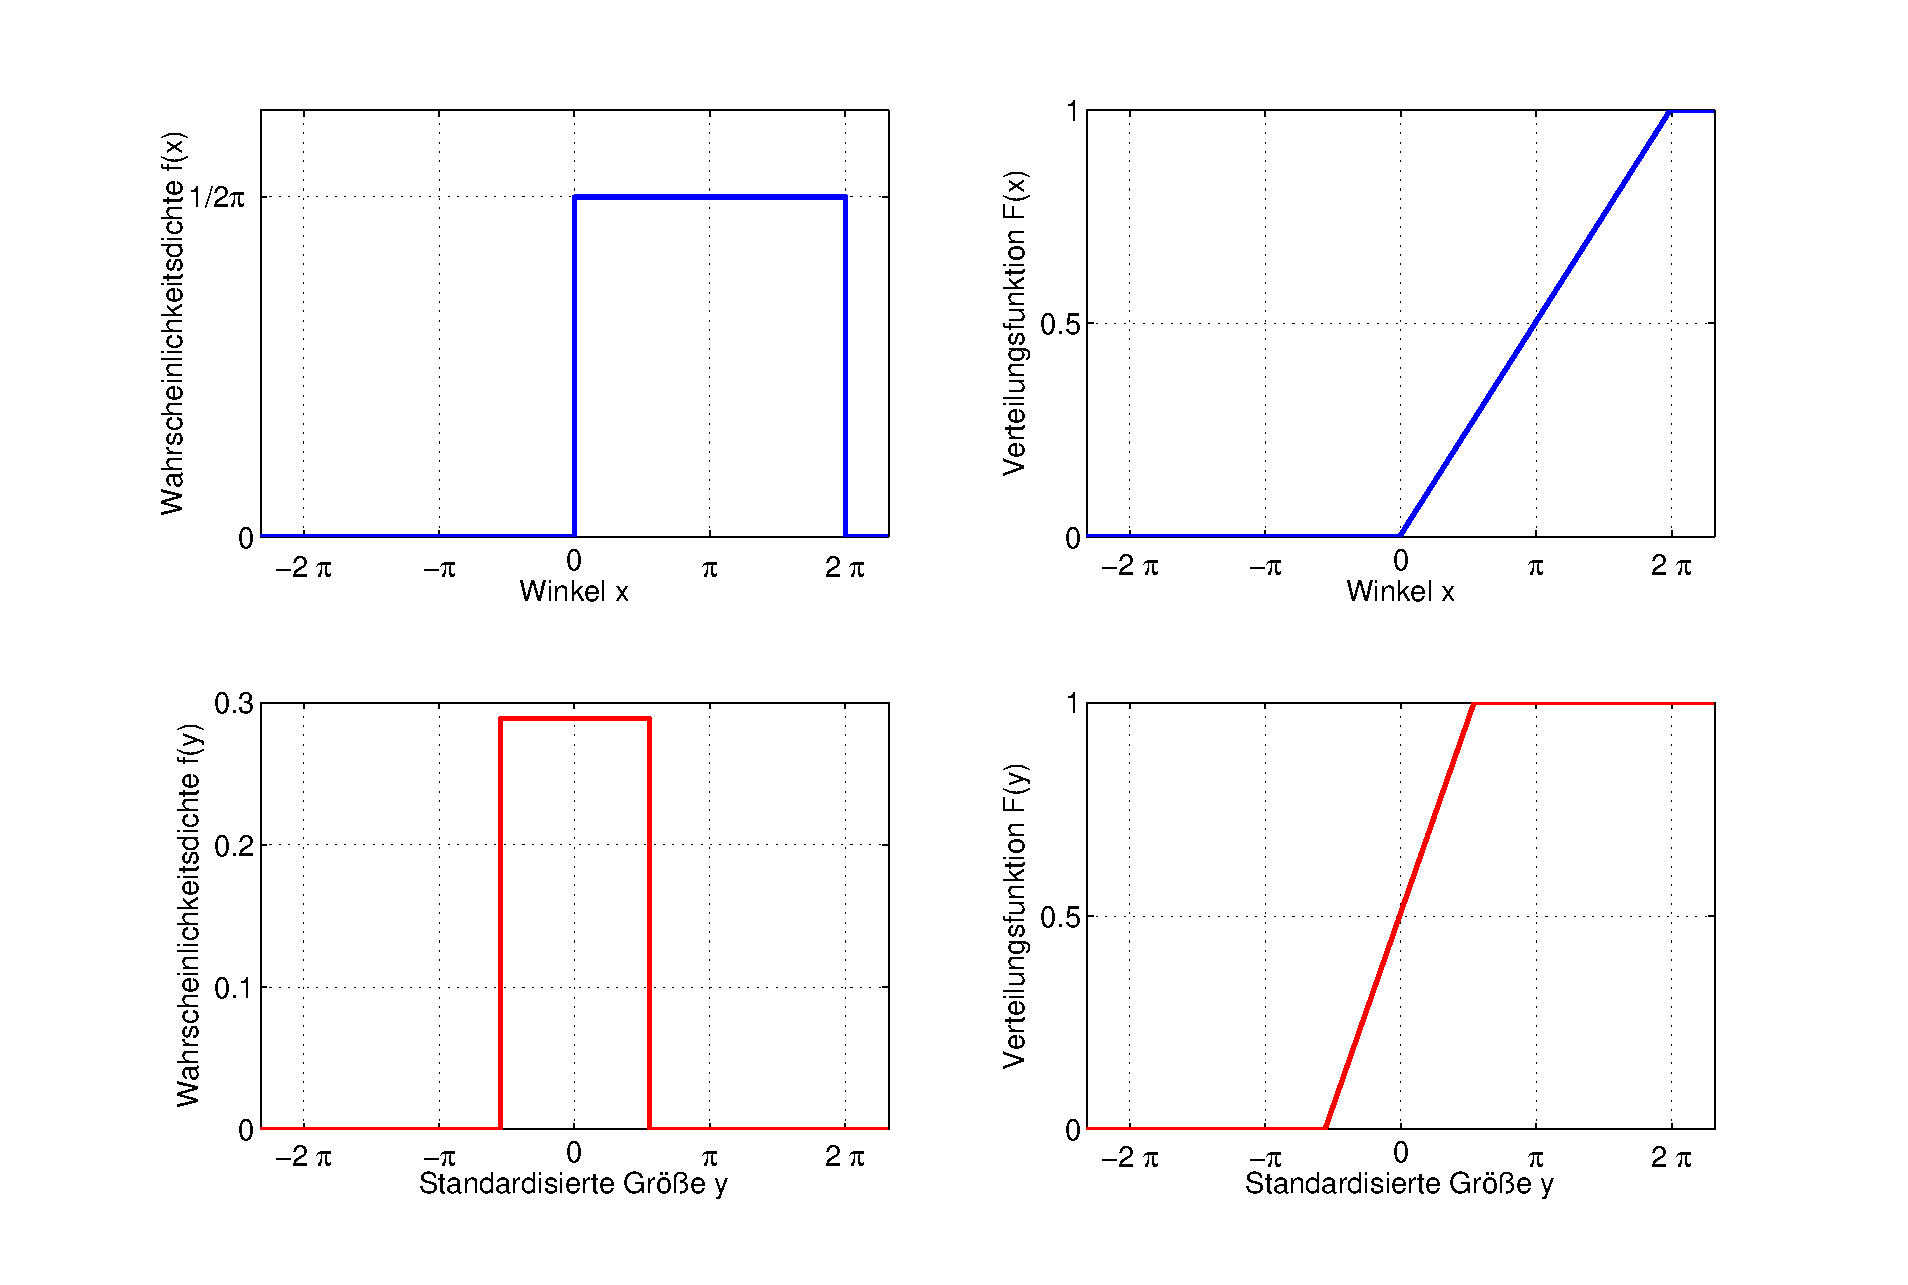
\includegraphics[width=1\textwidth]{Kapitel4/Bilder/image8}}
  \caption{Grafische Darstellung der Wahrscheinlichkeitsverteilung f\"{u}r das Beispiel Gl\"{u}cksrad mit und ohne Standardisierung}
  \label{fig:Standardisierung}
\end{figure}

\noindent Nach der Standardisierung der Zufallsvariable ist die Verteilung symmetrisch um den Mittelwert $\mu_{y}$ = 0. Die Varianz ergibt sich erwartungsgem\"{a}{\ss} zu

\begin{equation}\label{eq:fourhundrednine}
\sigma _{y}^{2} =\int _{-\infty}^{\infty}(y-\mu _{y})^{2} \cdot {f}\left(y\right){dy} =\int _{-\sqrt{3}}^{\sqrt{3}}y^{2} \cdot \dfrac{1}{2\cdot \sqrt{3}} {dy} =\dfrac{{\rm 1}}{2\cdot \sqrt{3}} \cdot \dfrac{1}{3} \cdot \left(3\cdot \sqrt{3} +3\cdot \sqrt{3} \right)=1
\end{equation}

\subsubsection{Generierung von Zufallszahlen mit einer definierten Verteilung}

\noindent In Programmen werden zur Generierung von Zufallszahlen Generatoren eingesetzt, die quasizuf\"{a}llig einen Wert 0 $\mathrm{<}$ x $\leq$ 1 erzeugen. Die Wahrscheinlichkeitsdichte dieser Zahlen ist typischerweise gleichverteilt.

\begin{equation}\label{eq:fourhundredten}
f_{X} (x)=1
\end{equation}

\noindent Die Zufallsvariable besitzt damit im Zahlenbereich 0 $\mathrm{<}$ x $\leq$ 1 die Verteilungsfunktion

\begin{equation}\label{eq:fourhundredeleven}
F_{X} (x)=x
\end{equation}

\noindent Um Zufallszahlen y mit einer beliebigen Verteilung F${}_{Y}$(y) zu generieren, wird die Funktion

\begin{equation}\label{eq:fourhundredtwelve}
y=F_{Y}^{-1} (x)
\end{equation}

\noindent berechnet. Nach Gleichung \eqref{eq:foureightysix} besitzt sie die Wahrscheinlichkeitsdichte

\begin{equation}\label{eq:fourhundredthirteen}
f_{X} \left(g^{-1} (y)\right)\cdot \left|\dfrac{dg^{-1} \left(y\right)}{dy} \right|=1\cdot \left|\dfrac{dF(y)}{dy} \right|=f_{Y} (y)
\end{equation}

\clearpage

\subsection{Spezielle diskrete Verteilungen}

\noindent Viele diskrete Fragestellungen der Wahrscheinlichkeitsrechnung lassen sich mit wenigen speziellen, diskreten Verteilungen beschreiben. Sie ergeben sich aus der Wahrscheinlichkeitstheorie und werden im Folgenden beschrieben.

\subsubsection{Diskrete Gleichverteilung}

\noindent Weisen bei einem Zufallsexperiment alle m\"{o}glichen Werte x$_{n}$ der Zufallsvariable x die gleiche Wahrscheinlichkeit p auf, ergibt sich aus der Bedingung f\"{u}r das sichere Ereignis

\begin{equation}\label{eq:fourhundredfourteen}
1=\sum _{n=1}^{N}f(x_{n}) =\sum _{n=1}^{N}p =N\cdot p
\end{equation}

\noindent Damit lautet die Wahrscheinlichkeitsverteilung 

\begin{equation}\label{eq:fourhundredfifteen}
f(x)=p=\dfrac{1}{N}
\end{equation}

\noindent und die Verteilungsfunktion berechnet sich zu

\begin{equation}\label{eq:fourhundredsixteen}
F(x)=\sum _{x_{n} =0}^{x}p =\sum _{x_{n} =0}^{x}\dfrac{1}{N}
\end{equation}

\noindent Zum Beispiel sind bei einem W\"{u}rfelexperiment mit einem regelm\"{a}{\ss}igen W\"{u}rfel die Wahrscheinlichkeiten f\"{u}r eine beliebige Augenzahl mit 

\begin{equation}\label{eq:fourhundredseventeen}
p=\dfrac{1}{6}
\end{equation}

\noindent gleichverteilt. Die Wahrscheinlichkeitsverteilung und Verteilungsfunktion der Gleichverteilung sind in Bild \ref{fig:Diskret_Gleichverteilung} dargestellt. Die Wahrscheinlichkeitsverteilung f(x) ist konstant, die Verteilungsfunktion F(x) nimmt an jeder Stelle, an der ein m\"{o}glicher Wert der Zufallsvariable steht, zu. 

\noindent 
\begin{figure}[H]
  \centerline{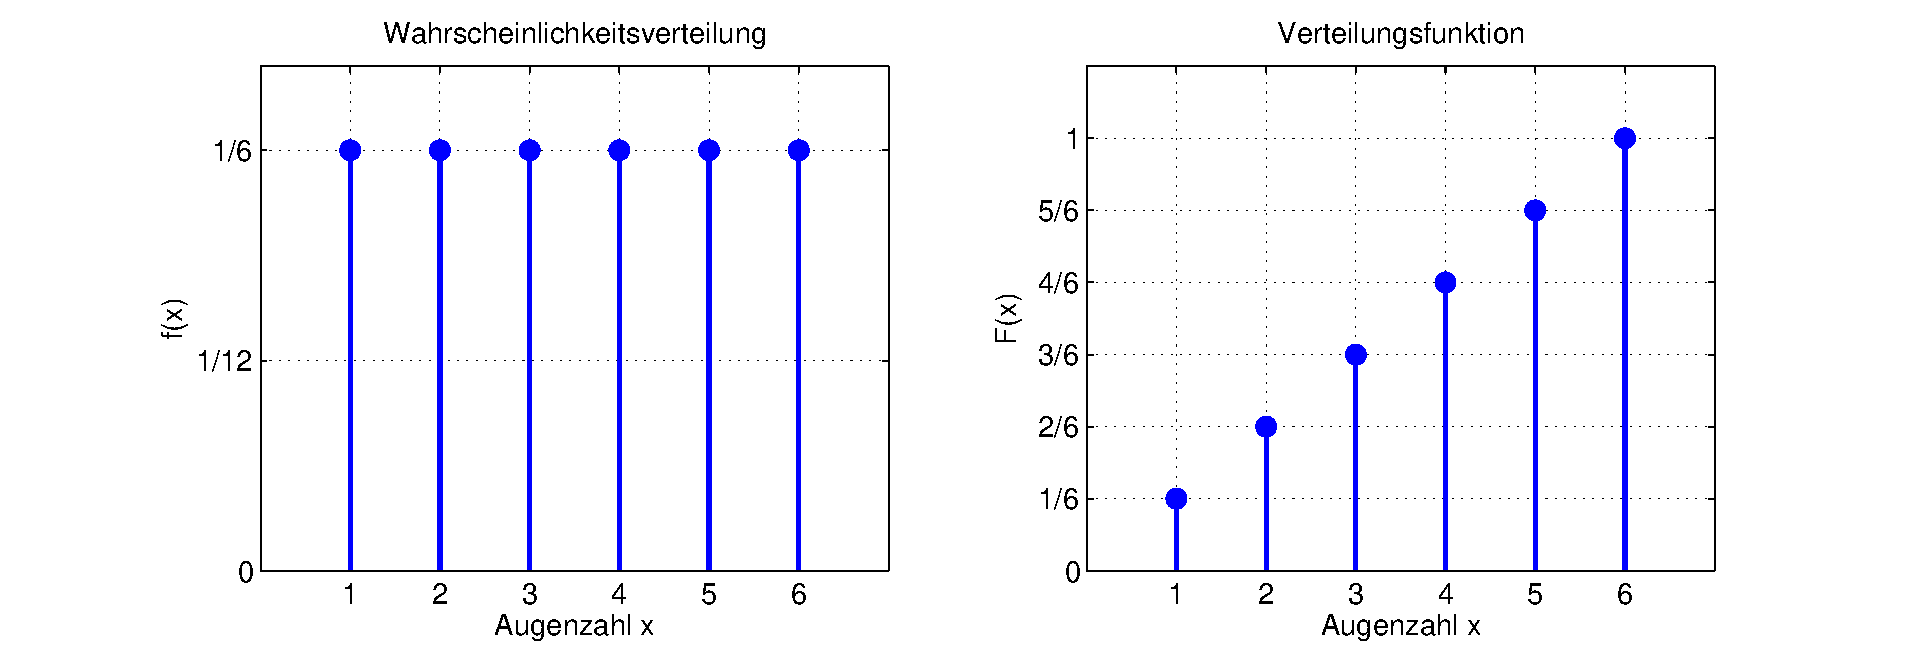
\includegraphics[width=1\textwidth]{Kapitel4/Bilder/image9}}
  \caption{Grafische Darstellung der Wahrscheinlichkeitsverteilung f(x) und Verteilungsfunktion F(x) f\"{u}r das W\"{u}rfeln einer Augenzahl x}
  \label{fig:Diskret_Gleichverteilung}
\end{figure}

\clearpage

\noindent Der Mittelwert der Gleichverteilung errechnet sich aus 

\begin{equation}\label{eq:fourhundredeighteen}
\mu =E(x)=\dfrac{1}{N} \cdot \sum _{n=1}^{N}x_{n}
\end{equation}

\noindent und die Varianz ergibt sich zu

\begin{equation}\label{eq:fourhundrednineteen}
\sigma ^{2} =E\left((x-\mu )^{2} \right)=\dfrac{1}{N} \cdot \sum _{n=1}^{N}(x_{n} -\mu)^{2} 
\end{equation}

\noindent
\colorbox{lightgray}{%
\arrayrulecolor{white}%
\renewcommand\arraystretch{0.6}%
\begin{tabular}{ wl{16.5cm} }
{\fontfamily{phv}\selectfont{Beispiel: Bewertung zweier Anlagem\"{o}glichkeiten}}
\end{tabular}%
}\medskip 

\noindent Dem Kunden einer Bank werden zur Geldanlage zwei m\"{o}gliche Anlagestrategien angeboten. Als konventionelle Variante steht eine Festgeldanlage mit einer festen Verzinsung von j\"{a}hrlich 3.33 \% zur Verf\"{u}gung. Als weitere Anlagevariante wird dem Kunden ein Modell auf Basis von Wertpapieren angeboten. Dabei wird in Abh\"{a}ngigkeit eines Wirtschaftsindex ein Zinssatz von 1.5, 2.5 oder 5 \% ausgezahlt. Da \"{u}ber den Verlauf des Wirtschaftsindex f\"{u}r das Anlagejahr keine Vorhersagen getroffen werden k\"{o}nnen, haben alle drei m\"{o}glichen Zinsbetr\"{a}ge eine gleich hohe Wahrscheinlichkeit, sie sind somit gleichverteilt. Bild \ref{fig:Diskret_Gleichverteilung_Anlagemoeglichkeiten} zeigt die resultierende Wahrscheinlichkeitsverteilung f(x) und die Verteilungsfunktion F(x).

\noindent 
\begin{figure}[H]
  \centerline{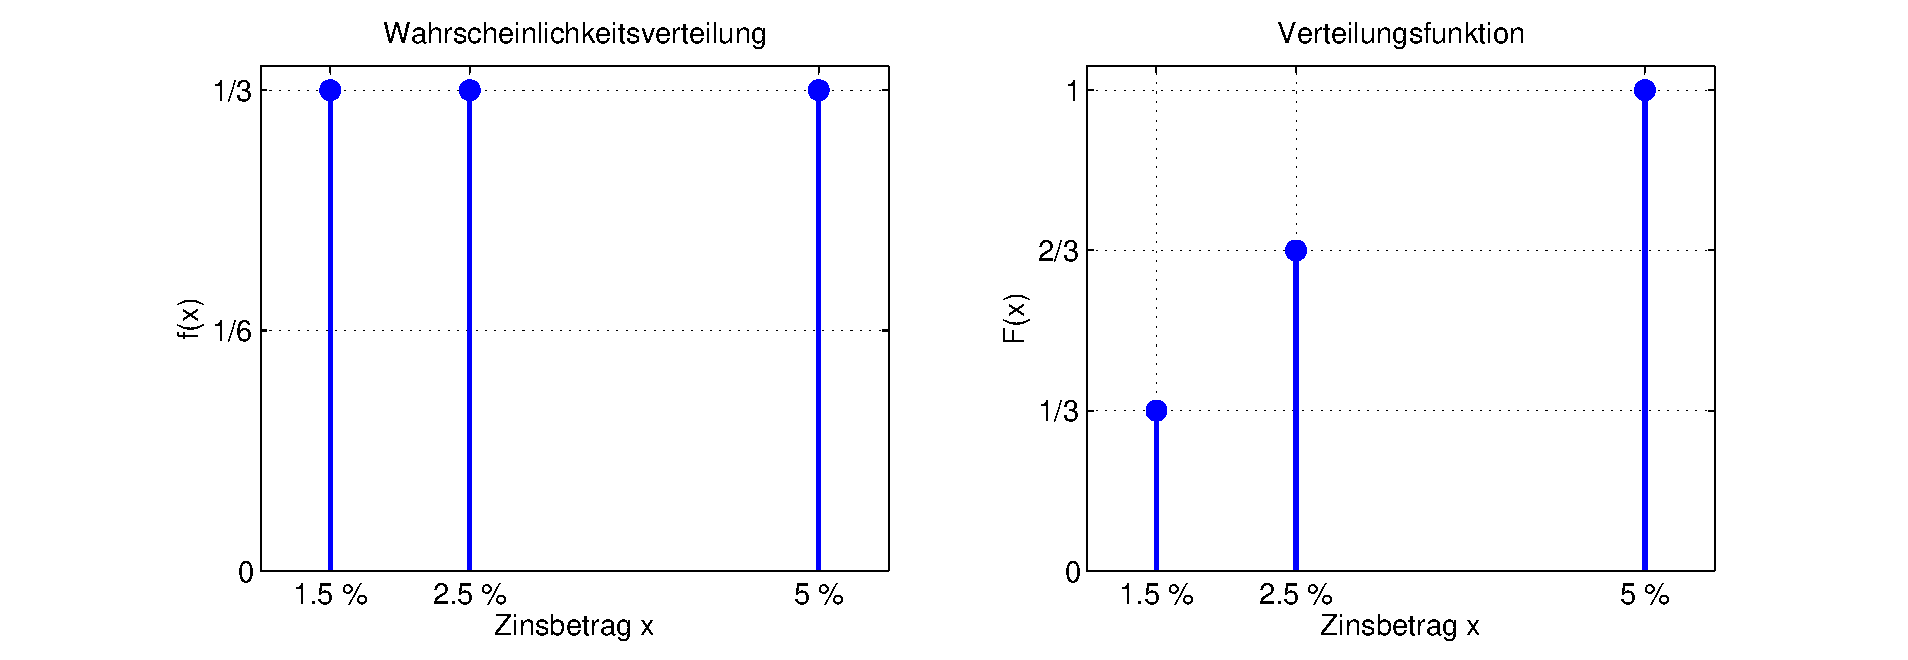
\includegraphics[width=1\textwidth]{Kapitel4/Bilder/image10}}
  \caption{Grafische Darstellung der Wahrscheinlichkeitsverteilung f(x) und Verteilungsfunktion F(x) f\"{u}r die Verzinsung bei Wertpapieren}
  \label{fig:Diskret_Gleichverteilung_Anlagemoeglichkeiten}
\end{figure}

\noindent Um zu entscheiden, bei welcher Anlagevariante mit h\"{o}heren Zinsertr\"{a}gen gerechnet werden kann, wird der Erwartungswert beziehungsweise der Mittelwert der zweiten Anlagevariante bestimmt. Dieser folgt zu

\begin{equation}\label{eq:fourhundredtwenty}
\mu =\dfrac{1}{N} \cdot \sum _{n=1}^{N}x_{n} =\dfrac{1}{3} \cdot (1.5+2.5+5)=3 \%
\end{equation}

\noindent Im Mittel wird der Kunde bei der Anlagevariante auf Basis des Wirtschaftsindex eine j\"{a}hrliche Verzinsung von 3 \% erhalten. Da die mittlere Zinserwartung bei h\"{o}herem Risiko geringer ist als bei der Festgeld-Anlage, ist die Festgeld-Anlage zu bevorzugen. 

\clearpage 

\noindent Die Erstellung von Bild \ref{fig:Diskret_Gleichverteilung_Anlagemoeglichkeiten} und die Berechnung des Mittelwertes wurde mit MATLAB durchgef\"{u}hrt.

\lstinputlisting[caption = {}]{Kapitel4/mat1.m}

\noindent Alternativ kann die Umsetzung in Python erfolgen.

\lstinputlisting[caption = {}]{Kapitel4/mat2.m}

\clearpage 

\subsubsection{Bernoulli-Verteilung}

\noindent Ein Spezialfall diskreter Verteilungen ist die Bernoulli-Verteilung, die ein Bernoulli Experiment beschreibt. Dabei wird gepr\"{u}ft, ob ein Ereignis bei einfacher Ausf\"{u}hrung des Experimentes eingetreten ist oder nicht. Die Zufallsvariable x ist damit definiert \"{u}ber

\begin{equation}\label{eq:fourhundredtwentyone}
x=\left\{\begin{array}{l} {1 \qquad \text{für das günstige Ereignis A}} \\ 
{0\qquad \text{für das ungünstige Ereignis A'}} \end{array}\right.
\end{equation}

\noindent Eine solche Variable wird als bin\"{a}re oder Bernoulli-Variable bezeichnet. Ist die Wahrscheinlichkeit f\"{u}r das g\"{u}nstige Ereignis A

\begin{equation}\label{eq:fourhundredtwentytwo}
P(A)=f(1)=p
\end{equation}

\noindent errechnet sich die Wahrscheinlichkeit f\"{u}r das ung\"{u}nstige Ereignis A' zu

\begin{equation}\label{eq:fourhundredtwentythree}
P(A')=f(0)=1-p=q
\end{equation}

\noindent Die Wahrscheinlichkeitsverteilung hat nur die beiden Werte p und q = 1 - p. Der Mittelwert der Bernoulli-Verteilung errechnet sich zu

\begin{equation}\label{eq:fourhundredtwentyfour}
\mu =E(x)=\sum _{n=1}^{2}x_{n} \cdot P(x_{n}) =0\cdot q+1\cdot p=p
\end{equation}

\noindent und die Varianz betr\"{a}gt 

\begin{equation}\label{eq:fourhundredtwentyfive}
\sigma ^{2} =E\left((x-\mu)^{2} \right)=E\left(x^{2} \right)-\mu ^{2} =p-p^{2} =p\cdot q
\end{equation}

\noindent Beispiele f\"{u}r Bernoulli-Experimente sind die Funktion von Bauelementen oder das Erf\"{u}llen von Spezifikationsmerkmalen. Bernoulli-Variablen erlauben jedoch nur eine grobe Kategorisierung von Ereignissen, eine feine Einteilung zum Beispiel nach der Frage, wie weit ein Grenzwert \"{u}berschritten wurde, k\"{o}nnen mit dem Bernoulli-Experiment nicht beantwortet werden.

\noindent
\colorbox{lightgray}{%
\arrayrulecolor{white}%
\renewcommand\arraystretch{0.6}%
\begin{tabular}{ wl{16.5cm} }
{\fontfamily{phv}\selectfont{Beispiel: Bit-Fehler bei der digitalen Signal\"{u}bertragung}}
\end{tabular}%
}\medskip 

\noindent Als Anwendungsbeispiel f\"{u}r die Bernoulli-Verteilung wird die \"{U}bertragung eines stochastischen 1-Bit-Bin\"{a}rsignals betrachtet, das den Zustand 0 oder 1 annehmen kann. Bei der \"{U}bertragung des Bits wird mit einem St\"{o}rsignal gerechnet, das eine \"{A}nderung des Zustandes mit einer Wahrscheinlichkeit von p = 0.25 bewirkt.\newline

\noindent Zur Darstellung wird die Zufallsvariable x definiert, die den Wert 1 annimmt, wenn das Bit w\"{a}hrend der \"{U}bertragung verf\"{a}lscht wurde und die den Wert 0 annimmt, wenn keine Verf\"{a}lschung vorliegt. Damit ergibt sich die Wahrscheinlichkeitsfunktion f(x) der Zufallsvariablen x zu

\begin{equation}\label{eq:fourhundredtwentysix}
f(x)=\left\{\begin{array}{l} {\dfrac{1}{4}\qquad \text{für } x=1} \\
\\
{\dfrac{3}{4}\qquad \text{für } x=0} \end{array}\right.
\end{equation}

\noindent Die Wahrscheinlichkeitsverteilung f(x) und die Verteilungsfunktion F(x) sind in Bild \ref{fig:Diskret_Bernoulli_Signaluebertragung} dargestellt.

\clearpage

\noindent 
\begin{figure}[H]
  \centerline{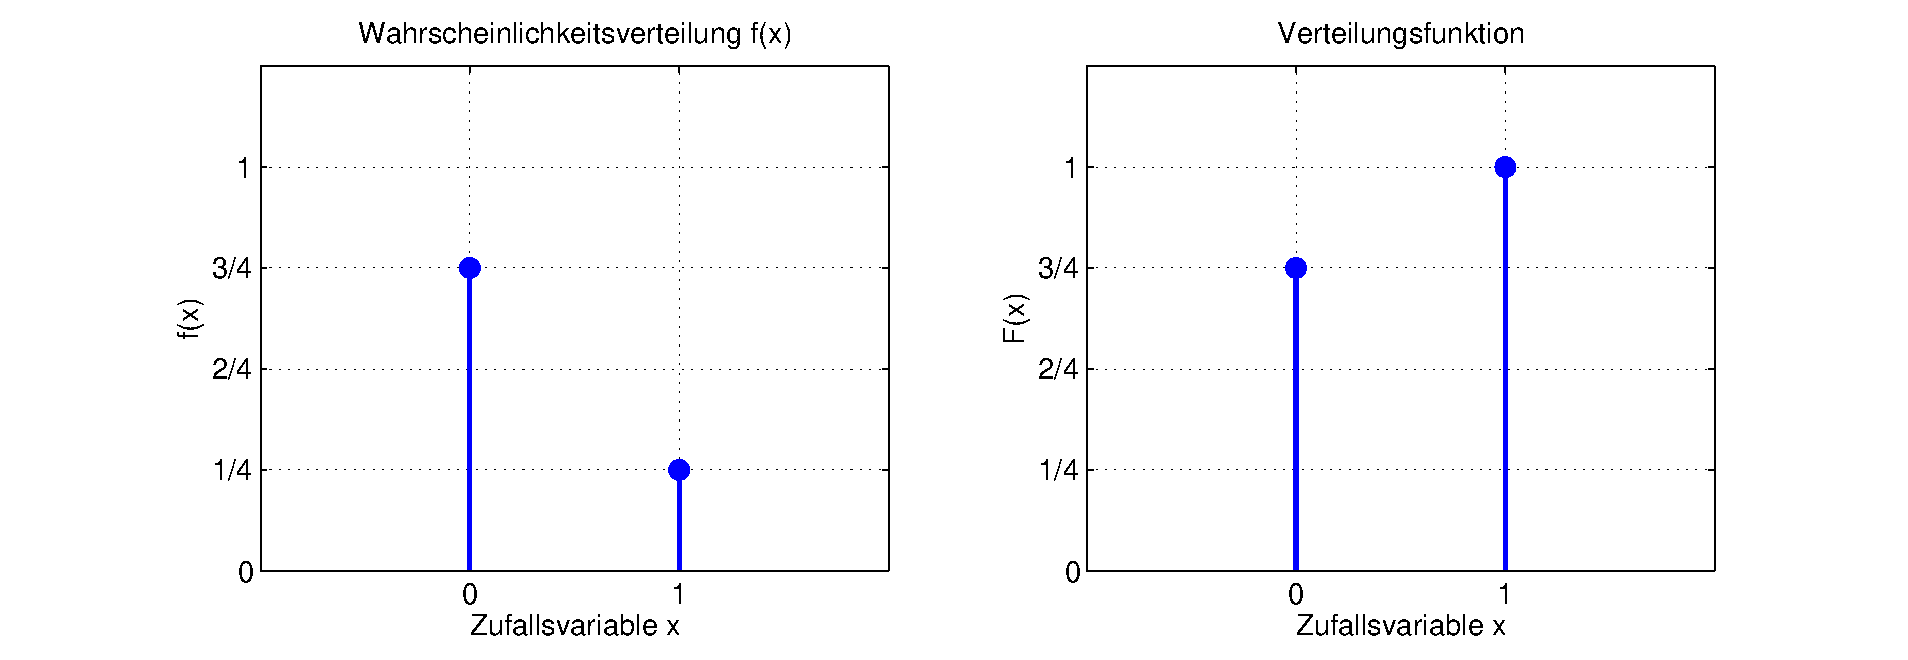
\includegraphics[width=1\textwidth]{Kapitel4/Bilder/image11}}
  \caption{Grafische Darstellung der Wahrscheinlichkeitsverteilung f(x) und Verteilungsfunktion F(x) einer Bernoulli-Verteilung einer 1-Bit-Bin\"{a}rsignal-\"{U}bertragung}
  \label{fig:Diskret_Bernoulli_Signaluebertragung}
\end{figure}

\subsubsection{Binomial-Verteilung}

\noindent Die Binomial-Verteilung ist eine Erweiterung der Bernoulli-Verteilung. Sie gibt an, wie viele g\"{u}nstige Ereignisse stattfinden, wenn ein Zufallsexperiment N-fach ausgef\"{u}hrt wird. Die Wahrscheinlichkeit f\"{u}r das Ereignis A ist bei jeder einzelnen Durchf\"{u}hrung konstant

\begin{equation}\label{eq:fourhundredtwentyseven}
P(A)=p
\end{equation}

\noindent Damit ergibt sich bei jeder einzelnen Durchf\"{u}hrung des Zufallsexperimentes f\"{u}r das inverse Ereignis A' die Wahrscheinlichkeit 

\begin{equation}\label{eq:fourhundredtwentyeight}
P(A')=1-p=q
\end{equation}

\noindent Bei einfacher Ausf\"{u}hrung (N = 1) kann die Zufallsvariable x nur die Werte 0 oder 1 annehmen. In dem Fall ergibt sich die Wahrscheinlichkeitsverteilung 

\begin{equation}\label{eq:fourhundredtwentynine}
f(x)=p^{x} \cdot q^{1-x}
\end{equation}

\noindent Wird das Zufallsexperiment N-fach ausgef\"{u}hrt, tritt das Ereignis A x-fach ein. Die Anzahl unterschiedlicher Anordnungen errechnet sich als Kombinationen ohne Wiederholungen zu (N \"{u}ber x). Die Wahrscheinlichkeitsverteilung bei N-facher Ausf\"{u}hrung des Zufallsexperiments ergibt sich damit aus dem Produkt der Realisierungsm\"{o}glichkeiten mit der Wahrscheinlichkeit f(x) des betreffenden Ereignisses. Sie folgt daher zu

\begin{equation}\label{eq:fourhundredthirty}
f(x)=\left(\begin{array}{l} {N} \\ 
{x} \end{array}\right)\cdot p^{x} \cdot q^{N-x}
\end{equation}

\noindent Gleichung \eqref{eq:fourhundredthirty} beschreibt die Wahrscheinlichkeit, dass ein Ereignis A bei N unabh\"{a}ngigen Ausf\"{u}hrungen des Experimentes x-mal eintritt, wenn das Ereignis A bei Einzelausf\"{u}hrung die konstante Wahrscheinlichkeit p besitzt und die Wahrscheinlichkeit des nicht Eintreffens q = 1 - p ist. Diese Verteilung wird als Binomial-Verteilung bezeichnet und ist in Bild \ref{fig:Diskret_Binomial1} f\"{u}r N = 16 und unterschiedliche Wahrscheinlichkeiten p dargestellt. In Abh\"{a}ngigkeit von N und p besitzt die Wahrscheinlichkeitsverteilung f(x) ein Maximum.

\clearpage

\noindent 
\begin{figure}[H]
  \centerline{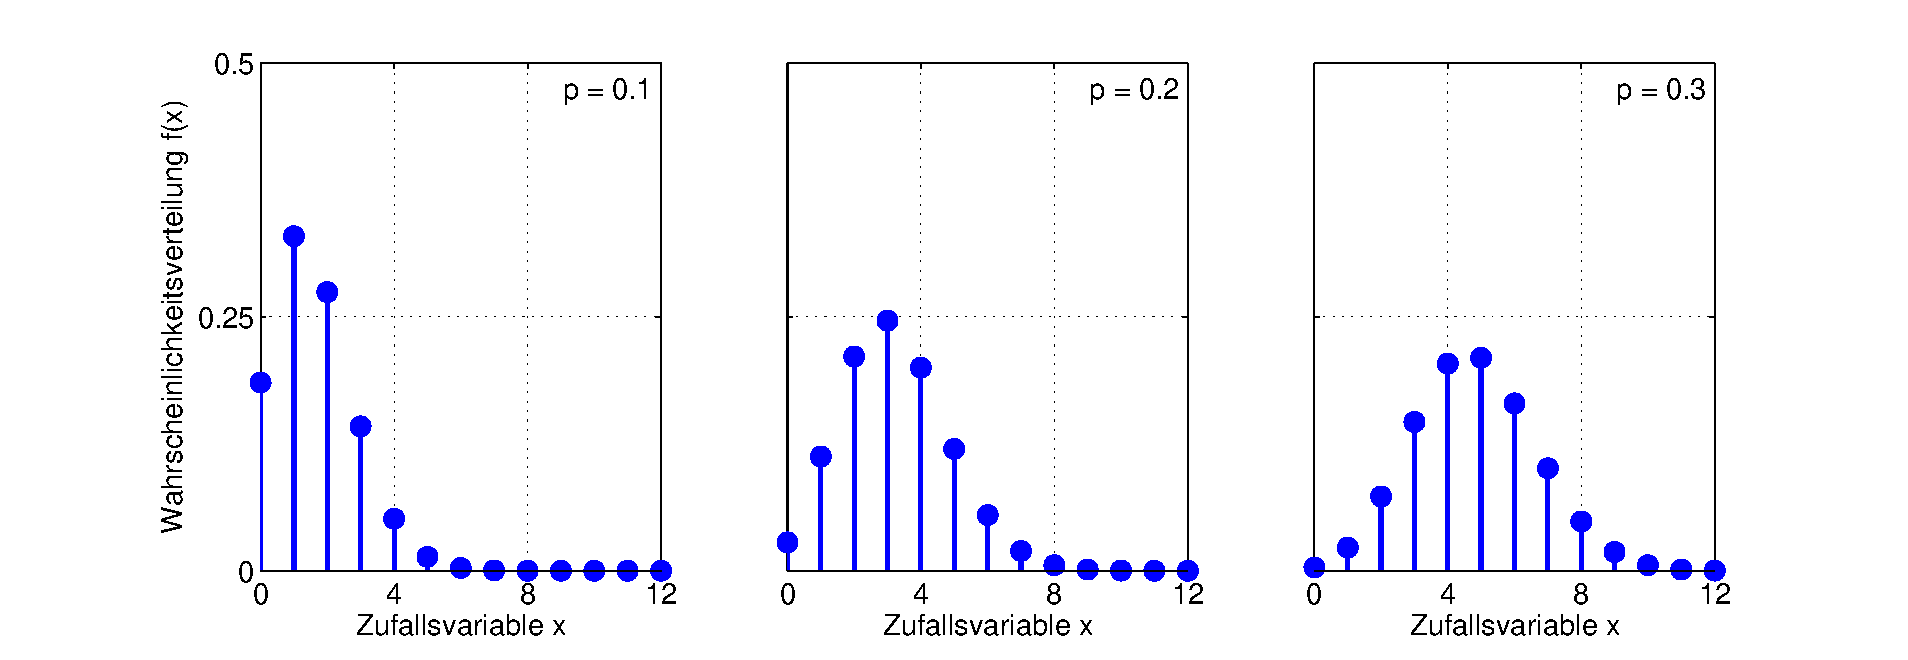
\includegraphics[width=1\textwidth]{Kapitel4/Bilder/image12}}
  \caption{Wahrscheinlichkeitsverteilung der Binomial-Verteilung mit N = 16 f\"{u}r unterschiedliche Erfolgswahrscheinlichkeiten p}
  \label{fig:Diskret_Binomial1}
\end{figure}

\noindent Die Verteilungsfunktion F(x) ergibt sich aus der Summe \"{u}ber die Wahrscheinlichkeitsverteilung zu

\begin{equation}\label{eq:fourhundredthirtyone}
F(x)=\sum _{x_{n} =0}^{x}\left(\begin{array}{l} {N} \\ 
{x_{n} } \end{array}\right)\cdot p^{x_{n}} \cdot q^{N-x_{n}} 
\end{equation}

\noindent Bild \ref{fig:Diskret_Binomial2} stellt die Wahrscheinlichkeitsverteilung f(x) und die Verteilungsfunktion F(x) der Binomial-Verteilung f\"{u}r N =16 und p = 0.2 dar.

\noindent 
\begin{figure}[H]
  \centerline{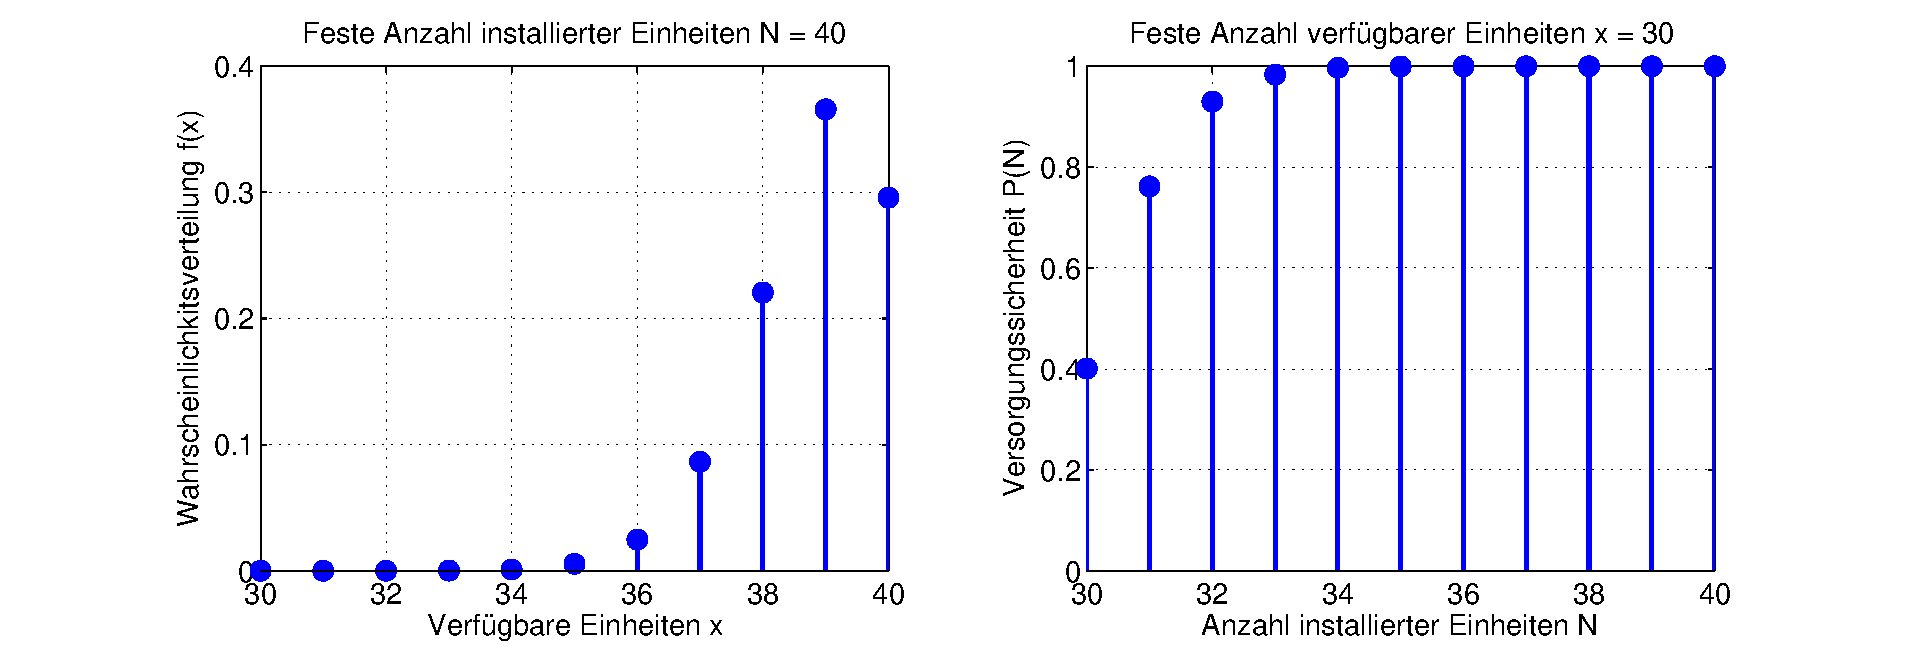
\includegraphics[width=1\textwidth]{Kapitel4/Bilder/image13}}
  \caption{Grafische Darstellung der Wahrscheinlichkeitsverteilung f(x) und Verteilungsfunktion F(x) einer Binomial-Verteilung mit p = 0.2}
  \label{fig:Diskret_Binomial2}
\end{figure}

\noindent Durch Auswerten der momenterzeugenden Funktion ergeben sich Mittelwert und Varianz der Binomial-Verteilung zu

\begin{equation}\label{eq:fourhundredthirtytwo}
\mu =N\cdot p
\end{equation}

\noindent und

\begin{equation}\label{eq:fourhundredthirtythree}
\sigma ^{2} =N\cdot p\cdot q
\end{equation}

\noindent Mit der Einf\"{u}hrung von Funktionen mehrerer Zufallsvariablen wird sich zeigen, dass sich Mittelwert und Varianz der Binomial-Verteilung aus der Summe von N Mittelwerten beziehungsweise N Varianzen der Bernoulli-Verteilung ergeben.

\clearpage

\noindent
\colorbox{lightgray}{%
\arrayrulecolor{white}%
\renewcommand\arraystretch{0.6}%
\begin{tabular}{ wl{16.5cm} }
{\fontfamily{phv}\selectfont{Beispiel: Versorgungssicherheit}}
\end{tabular}%
}\medskip 

\noindent Eine wichtige Aufgabe der Energieversorgungsunternehmen ist die Versorgung mit einer fiktiven Sicherheit von 99.9 \% sicherzustellen. Um bei dem Ausfall einzelner Einspeiseeinheiten ausreichend elektrische Leistung zur Verf\"{u}gung stellen zu k\"{o}nnen, werden Reserveeinheiten vorgehalten. Als Grundlage f\"{u}r die Berechnung dieses Beispiels wird ein fiktives Verbundnetz mit N = 30 erforderlichen Einspeiseeinheiten und einer unabh\"{a}ngigen Verf\"{u}gbarkeitswahrscheinlichkeit jeder Einheit von p = 97 \% angenommen. Die Wahrscheinlichkeit f\"{u}r die Verf\"{u}gbarkeit von x der N installierten Einheiten wird durch die Binomial-Verteilung beschrieben.

\begin{equation}\label{eq:fourhundredthirtyfour}
f(x)=\left(\begin{array}{l} {N} \\ 
\end{array}\right)\cdot p^{x} \cdot (1-p)^{N-x}
\end{equation}

\noindent Bild \ref{fig:Diskret_Binomial_Versorgungssicherheit} zeigt links die Verf\"{u}gbarkeitswahrscheinlichkeit von x Einheiten bei N = 40 installierten Einheiten. Es m\"{u}ssen mindestens 30 Einheiten verf\"{u}gbar sein, es d\"{u}rfen aber auch mehr sein. Damit ergibt sich die gesuchte Wahrscheinlichkeit zu

\begin{equation}\label{eq:fourhundredthirtyfive}
P(x\ge 30)=1-F(29)=1-\sum _{x_{n} =0}^{29}\left(\begin{array}{l} {N} \\ 
{x_{n} } \end{array}\right)\cdot 0.97^{x_{n}} \cdot 0.03^{N-x_{n}}  \ge 0.999
\end{equation}

\noindent Die Anzahl installierter Einheiten N muss so gro{\ss} sein, dass sich die Versorgungssicherheit von 99.9 \% erreicht wird. Bild \ref{fig:Diskret_Binomial_Versorgungssicherheit} zeigt im rechten Bildteil die Versorgungssicherheit als Funktion der installierten Einheiten N. 

\noindent 
\begin{figure}[H]
  \centerline{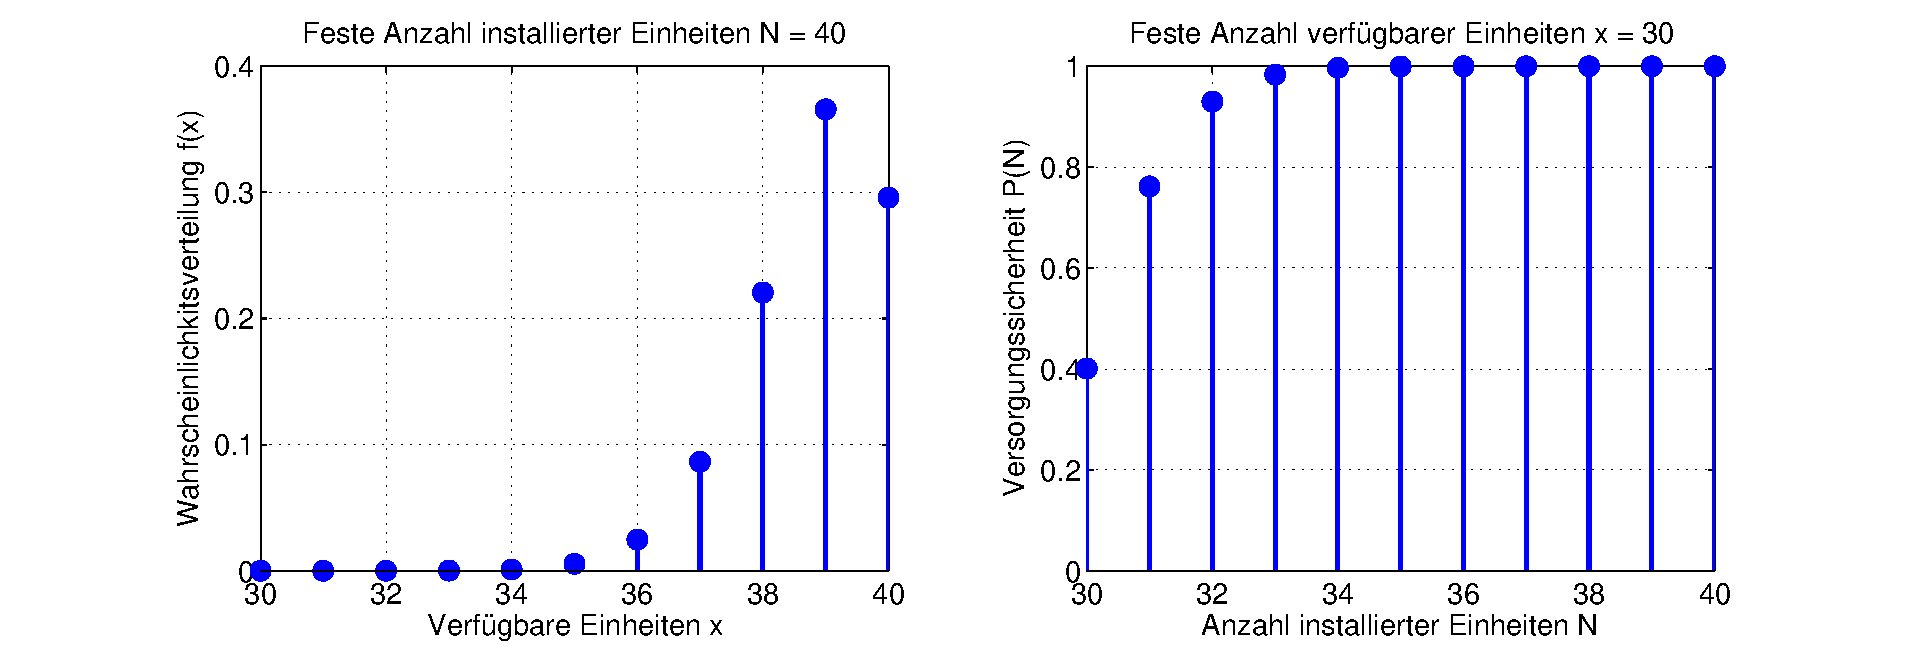
\includegraphics[width=1\textwidth]{Kapitel4/Bilder/image14}}
  \caption{Grafische Darstellung der Verf\"{u}gbarkeitswahrscheinlichkeit von x bei N = 40 installierten Einheiten und der Versorgungssicherheit als Funktion der installierten Einheiten N}
  \label{fig:Diskret_Binomial_Versorgungssicherheit}
\end{figure}

\noindent Eine numerische Auswertung zeigt, dass mindestens 35 Einheiten installiert werden m\"{u}ssen, um die Versorgungssicherheit mit einer Wahrscheinlichkeit von 99.9 \% sicherzustellen.\newline

\noindent Mit MATLAB kann die Versorgungssicherheit f\"{u}r das definierte Verbundnetz berechnet werden.

\lstinputlisting[caption = {}]{Kapitel4/mat3.m}

\clearpage

\noindent Alternativ kann die Versorgungssicherheit in Python umgesetzt werden.

\lstinputlisting[caption = {}]{Kapitel4/mat4.m}

\noindent Ein weiteres typisches Anwendungsbeispiel f\"{u}r die Binomial-Verteilung ist die Qualit\"{a}tskontrolle. Sind zum Beispiel in einem Beh\"{a}lter M Schrauben und sind davon G Schrauben defekt, so ist die Wahrscheinlichkeit p, eine defekte Schraube zu ziehen 

\begin{equation}\label{eq:fourhundredthirtysix}
p=\dfrac{G}{M} 
\end{equation}

\noindent Nach dem Ziehen wird die Schraube wieder zur\"{u}ckgelegt. Damit \"{a}ndert sich die Wahrscheinlichkeit p nicht und die Wahrscheinlichkeit, bei N Z\"{u}gen mit Zur\"{u}cklegen genau x defekte Schrauben zu ziehen, berechnet sich aus

\begin{equation}\label{eq:fourhundredthirtyseven}
f(x)=\left(\begin{array}{l} {N} \\ 
{x} \end{array}\right)\cdot \left(\dfrac{G}{M} \right)^{x} \cdot \left(1-\dfrac{G}{M} \right)^{n-x}
\end{equation}

\noindent Praktisch gesehen ist das Ziehen ohne Zur\"{u}cklegen wichtiger als das Ziehen mit Zur\"{u}cklegen. Die mathematische Beschreibung mithilfe der hypergeometrischen Verteilung ist jedoch anspruchsvoller, da sich die Erfolgswahrscheinlichkeit p w\"{a}hrend des Experimentes \"{a}ndert.

\subsubsection{Hypergeometrische Verteilung}

\noindent In Abschnitt 4.5.3 wird die Binomial-Verteilung zur Beschreibung von Zufallsexperimenten mit gleichbleibender Wahrscheinlichkeit p vorgestellt. Werden zum Beispiel bei der Eingangskontrolle die \"{u}berpr\"{u}ften Gegenst\"{a}nde nicht zur\"{u}ckgelegt, \"{a}ndert sich die Wahrscheinlichkeit p im Laufe des Zufallsexperiments. Die Wahrscheinlichkeitsverteilung bei n-facher Ausf\"{u}hrung des Zufallsexperiments kann in diesem Fall mit der hypergeometrischen Verteilung beschrieben werden.\newline

\noindent Zur Herleitung der Wahrscheinlichkeitsverteilung wird davon ausgegangen, dass sich in einem Beh\"{a}lter M Elemente befinden, von denen G Elemente defekt sind. Es wird eine Stichprobe von N Elementen ausgew\"{a}hlt. Die Reihenfolge ist nicht relevant. Nach den Gleichungen zu Kombinationen aus Kapitel 2 kann aus einer Grundgesamtheit von M Elementen eine Teilmenge von N Elementen auf (M \"{u}ber N) M\"{o}glichkeiten gew\"{a}hlt werden. Entsprechend lassen sich aus G defekten Elementen x defekte Elemente auf (G \"{u}ber x) M\"{o}glichkeiten ausw\"{a}hlen und G - x brauchbare Elemente lassen sich aus M - G brauchbaren Elementen auf ((M - G) \"{u}ber (G - x)) Weisen ziehen.\newline

\noindent Damit wird die Wahrscheinlichkeit, bei einer N-fachen Ziehung ohne Zur\"{u}cklegen x defekte Elemente zu finden, mit der Wahrscheinlichkeitsverteilung 

\begin{equation}\label{eq:fourhundredthirtyeight}
f(x)=\dfrac{\left(\begin{array}{l} {G} \\ 
{x} \end{array}\right)\cdot \left(\begin{array}{l} {M-G} \\ 
{G-x} \end{array}\right)}{\left(\begin{array}{l} {M} \\ 
{N} \end{array}\right)}
\end{equation}

\noindent beschrieben. Die Verteilungsfunktion F(x) der hypergeometrischen Verteilung ergibt sich durch Summation der Wahrscheinlichkeitsverteilung.

\begin{equation}\label{eq:fourhundredthirtynine}
F\left(x\right)=\sum _{x_{n} =-\infty }^{x}\left(\dfrac{\left(\begin{array}{l} {G} \\ {x_{n} } \end{array}\right)\cdot \left(\begin{array}{l} {M-G} \\ {G-x_{n} } \end{array}\right)}{\left(\begin{array}{l} {M} \\ {N} \end{array}\right)} \right)
\end{equation}

\noindent Der Mittelwert der hypergeometrischen Verteilung betr\"{a}gt 

\begin{equation}\label{eq:fourhundredfourty}
\mu =N\cdot \dfrac{G}{M}
\end{equation}

\noindent und entspricht dem Mittelwert der Binomial-Verteilung. Die Varianz der hypergeometrischen Verteilung ergibt sich aus

\begin{equation}\label{eq:fourhundredfourtyone}
\sigma ^{2} =\dfrac{N\cdot G\cdot (M-G)\cdot (M-N)}{M^{2} \cdot (M-1)}
\end{equation}

\noindent Sowohl die Wahrscheinlichkeitsverteilung f(x) als auch die Verteilungsfunktion F(x) der Hypergeometrischen Verteilung mit den Parametern G = 8, M = 16 und N = 8 ist in Bild \ref{fig:Diskret_Hypergeometrisch1} abgebildet.

\noindent 
\begin{figure}[H]
  \centerline{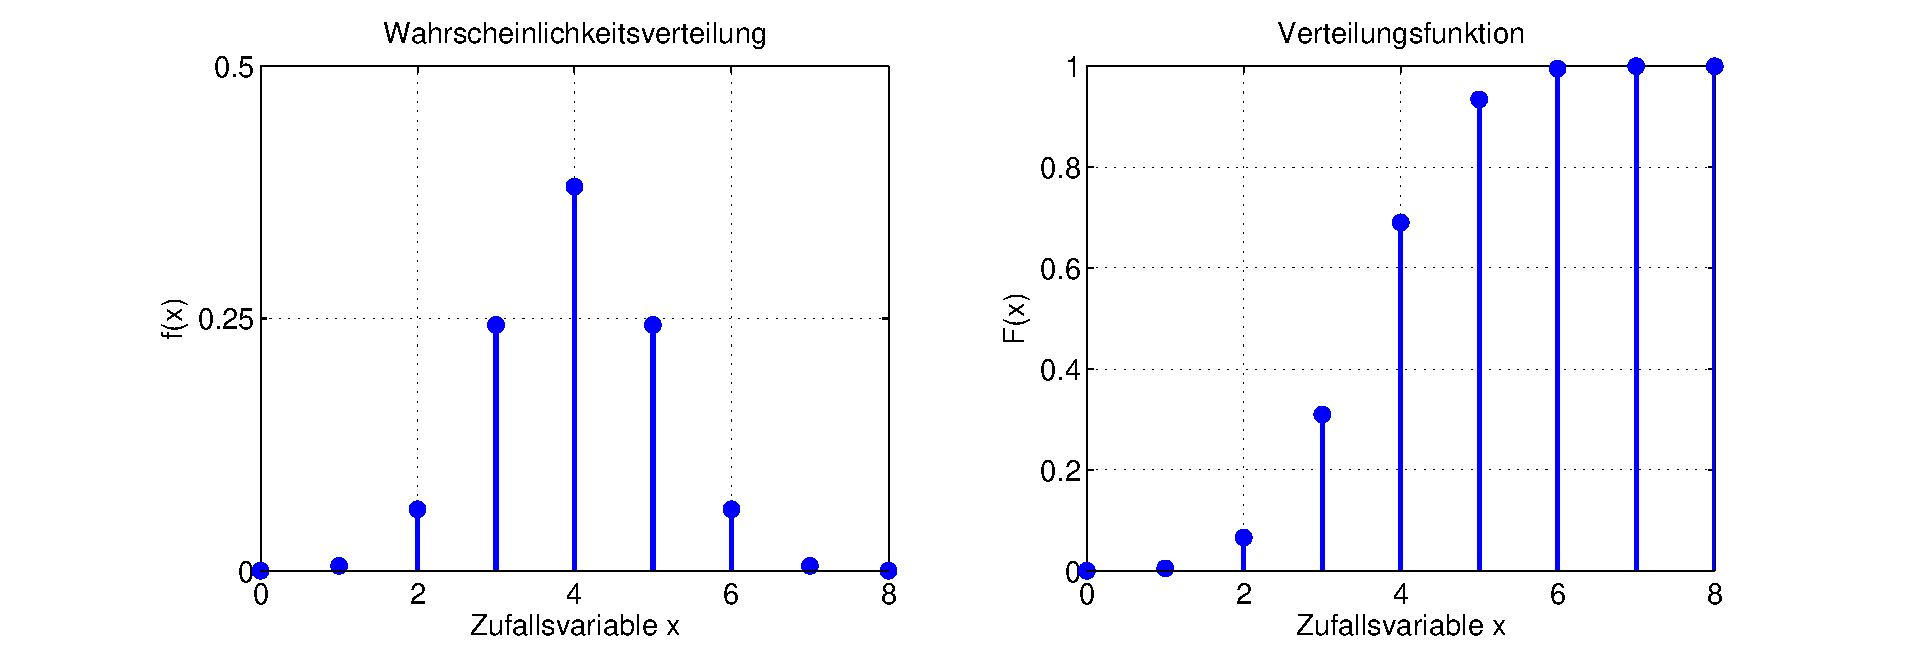
\includegraphics[width=1\textwidth]{Kapitel4/Bilder/image15}}
  \caption{Darstellung der Wahrscheinlichkeitsverteilungen f(x) und der Verteilungsfunktion F(x) f\"{u}r die Hypergeometrische Verteilung mit G = 8, M = 16 und N = 8}
  \label{fig:Diskret_Hypergeometrisch1}
\end{figure}

\noindent
\colorbox{lightgray}{%
\arrayrulecolor{white}%
\renewcommand\arraystretch{0.6}%
\begin{tabular}{ wl{16.5cm} }
{\fontfamily{phv}\selectfont{Beispiel: Qualit\"{a}tssicherung}}
\end{tabular}%
}\medskip 

\noindent Die hypergeometrische Verteilung wird mit einem Beispiel zur Qualit\"{a}tssicherung vertieft. Eine Firma liefert Dichtungen in Packungen zu je 100 St\"{u}ck. Eine Packung darf laut Liefervertrag h\"{o}chstens 10 \% Ausschuss enthalten. Jede Packung wird gepr\"{u}ft, indem 10 St\"{u}ck zuf\"{a}llig und ohne Zur\"{u}cklegen entnommen werden. Sind diese 10 St\"{u}ck alle einwandfrei, wird die Packung angenommen. Anderenfalls wird sie zur\"{u}ckgewiesen. Es soll die Frage untersucht werden, wie gro{\ss} bei diesem Pr\"{u}fverfahren die Wahrscheinlichkeit ungerechtfertigter Reklamationen ist, bei der eine Packung zur\"{u}ckgewiesen wird, obwohl sie den Lieferbedingungen entspricht.\newline

\noindent Bei h\"{o}chstens 10 \% Ausschuss darf eine Packung mit M = 100 Dichtungen maximal G = 10 fehlerhafte St\"{u}cke enthalten, um gerade noch den Spezifikationen zu entsprechen. Zur Berechnung der Wahrscheinlichkeit einer ungerechtfertigten Zur\"{u}ckweisung wird zun\"{a}chst die Wahrscheinlichkeit daf\"{u}r bestimmt, dass sich unter N = 10 Ringen kein fehlerhaftes St\"{u}ck befindet. Mit der Hypergeometrischen Verteilung ergibt sich diese zu

\begin{equation}\label{eq:fourhundredfourtytwo}
f(0)=\dfrac{\left(\begin{array}{c} {10} \\ 
{0} \end{array}\right)\cdot \left(\begin{array}{c} {90} \\ 
{10} \end{array}\right)}{\left(\begin{array}{c} {100} \\ 
{10} \end{array}\right)} =0.33
\end{equation}

\noindent Die Wahrscheinlichkeit f\"{u}r eine ungerechtfertigte Reklamation betr\"{a}gt 

\begin{equation}\label{eq:fourhundredfourtythree}
P=1-f(0)=1-0.33=0.67
\end{equation}

\noindent Sie ist in diesem Fall mit 67 \% sehr hoch und ist deshalb f\"{u}r eine qualifizierte Eingangskontrolle nicht zielf\"{u}hrend. Die Berechnung der Wahrscheinlichkeit erfolgt mit MATLAB durch folgendes Programm.


\lstinputlisting[caption = {}]{Kapitel4/mat5.m}

\noindent Alternativ kann die Eingangskontrolle in Python berechnet werden.

\lstinputlisting[caption = {}]{Kapitel4/mat6.m}

\noindent Die Hypergeometrische Verteilung kann unter bestimmten Bedingungen in die Binomial-Verteilung \"{u}berf\"{u}hrt werden. Bild \ref{fig:Diskret_Hypergeometrisch2} vergleicht die Binomial-Verteilung aus Abschnitt 4.5.3 mit der Hypergeometrischen Verteilung f\"{u}r unterschiedliche Verh\"{a}ltnisse der Anzahl G an Gutteilen zur Gesamtmenge M und dem Umfang der Stichprobe N. Die Approximation der hypergeometrischen Verteilung durch die Binomial-Verteilung verbessert sich mit sinkendem Verh\"{a}ltnis des Stichprobenumfangs N zur Grundgesamtheit M und sinkender Erfolgswahrscheinlichkeit p = G/M.

\noindent 
\begin{figure}[H]
  \centerline{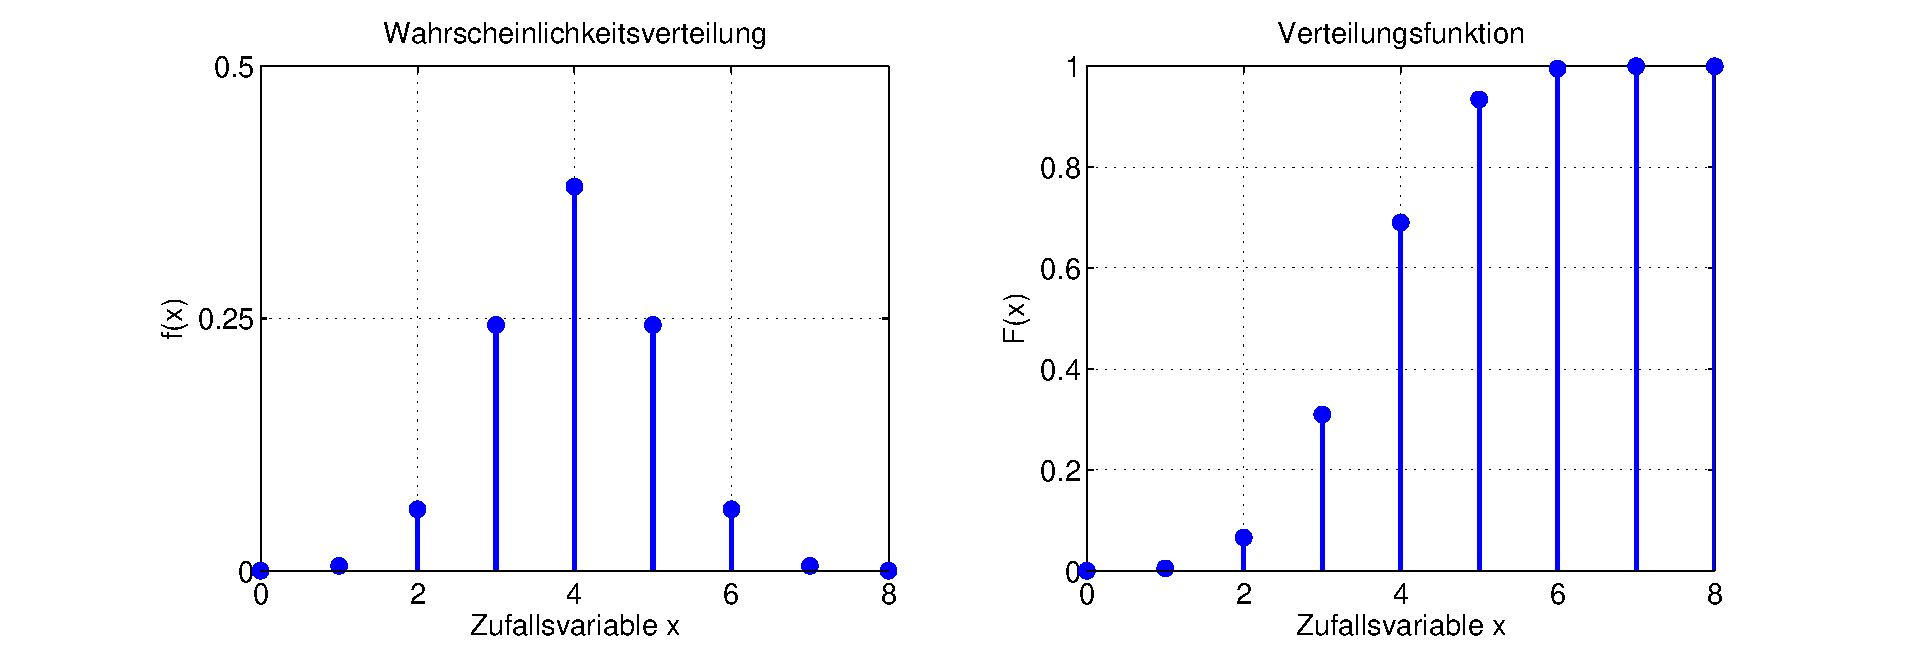
\includegraphics[width=1\textwidth]{Kapitel4/Bilder/image15}}
  \caption{Grafischer Vergleich der Wahrscheinlichkeitsverteilungen f\"{u}r die Binomial- und die hypergeometrische Verteilung}
  \label{fig:Diskret_Hypergeometrisch2}
\end{figure}

\subsubsection{Poisson-Verteilung}

\noindent Ist die konstante Erfolgswahrscheinlichkeit p bei einem einzelnen Experiment klein und die Anzahl N der Ausf\"{u}hrungen sehr gro{\ss}, wird das Rechnen mit der Binomial-Verteilung wegen der Binomial-Koeffizienten aufwendig. F\"{u}r den Fall p $\rightarrow$ 0 kann die Binomial-Verteilung durch die Poisson-Verteilung approximiert werden. Dabei soll der Mittelwert 

\begin{equation}\label{eq:fourhundredfourtyfour}
\mu =N\cdot p
\end{equation}

\noindent erhalten bleiben. F\"{u}r die Erfolgswahrscheinlichkeit p und die Wahrscheinlichkeit des Misserfolgs q gilt mit dieser Annahme

\begin{equation}\label{eq:fourhundredfourtyfive}
p=\dfrac{\mu}{N}
\end{equation}

\noindent beziehungsweise

\begin{equation}\label{eq:fourhundredfourtysix}
q=1-p=1-\dfrac{\mu}{N}
\end{equation}

\noindent Durch Einsetzen dieser Beziehungen in die Definitionsgleichung der Binomial-Verteilung aus Gleichung \eqref{eq:fourhundredthirteen} ergibt sich 

\begin{equation}\label{eq:fourhundredfourtyseven}
f\left(x\right)=\left(\begin{array}{l} {N} \\
{x} \end{array}\right)\cdot p^{x} \cdot q^{n-x} =\left(\begin{array}{l} {N} \\
{x} \end{array}\right)\cdot \left(\dfrac{\mu }{N} \right)^{x} \cdot \left(1-\dfrac{\mu }{N} \right)^{N-x}
\end{equation}

\noindent F\"{u}r den Grenz\"{u}bergang N $\rightarrow$ $\infty$ ergibt sich die Poisson-Verteilung [Krey91] mit der Wahrschein\"{o}ichkeitsverteilung

\begin{equation}\label{eq:fourhundredfourtyeight}
f(x)=\dfrac{\mu ^{x}}{x!} \cdot e^{-\mu}
\end{equation}

\noindent und der Verteilungsfunktion

\begin{equation}\label{eq:fourhundredfourtynine}
F(x)=\sum _{x_{n} =0}^{x}\dfrac{\mu ^{x_{n}}}{x_{n} !} \cdot e^{-\mu}
\end{equation}

\noindent Bild \ref{fig:Diskret_Poisson} vergleicht die Binomial- und die Poisson-Verteilung f\"{u}r unterschiedliche Erfolgswahrscheinlichkeiten p und Stichprobenumf\"{a}nge N.

\clearpage

\noindent 
\begin{figure}[H]
  \centerline{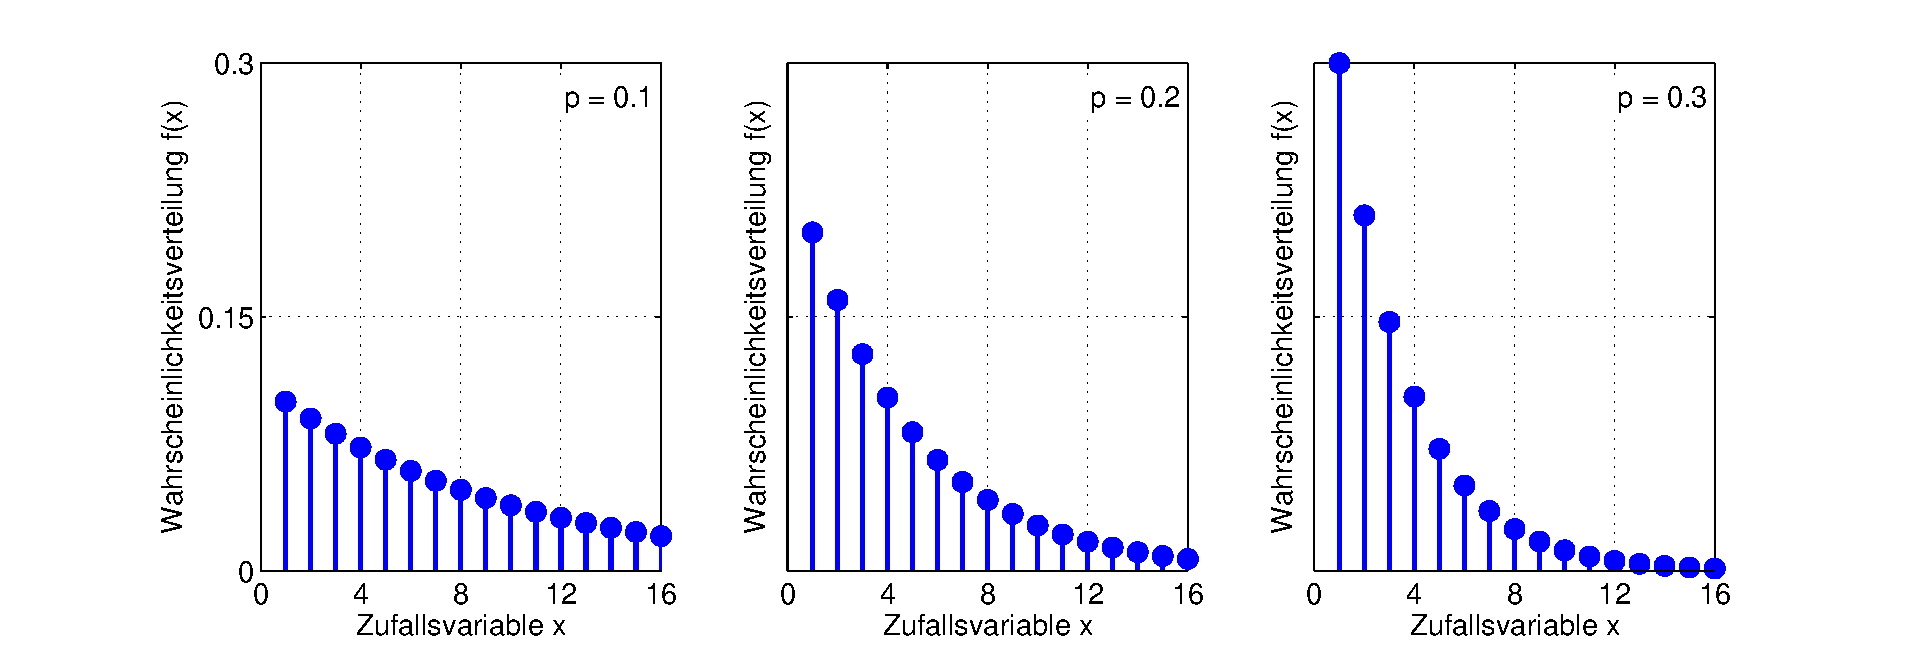
\includegraphics[width=1\textwidth]{Kapitel4/Bilder/image18}}
  \caption{Grafischer Vergleich der Wahrscheinlichkeitsverteilung f(x) f\"{u}r die Binomial- und die Poisson-Verteilung}
  \label{fig:Diskret_Poisson}
\end{figure}

\noindent Die Approximation der Binomial-Verteilung durch die Poisson-Verteilung verbessert sich mit steigendem Umfang N der Stichprobe und sinkender Erfolgswahrscheinlichkeit p. Der Mittelwert ist definitionsgem\"{a}{\ss} identisch zu dem Mittelwert der Binomial-Verteilung

\begin{equation}\label{eq:fourhundredfifty}
\mu =N\cdot p
\end{equation}

\noindent Durch Auswerten der momenterzeugenden Funktion ergibt sich die Varianz der Poisson-Verteilung zu

\begin{equation}\label{eq:fourhundredfiftyone}
\sigma ^{2} =N\cdot p=\mu
\end{equation}

\noindent
\colorbox{lightgray}{%
\arrayrulecolor{white}%
\renewcommand\arraystretch{0.6}%
\begin{tabular}{ wl{16.5cm} }
{\fontfamily{phv}\selectfont{Beispiel: Fertigung von Widerst\"{a}nden}}
\end{tabular}%
}\medskip 

\noindent Als Beispiel wird die Fertigung von Widerst\"{a}nden untersucht. Die Widerst\"{a}nde mit einem Nennwert von 50 $\Omega$ werden in Packungen zu je 100 St\"{u}ck geliefert. Dabei wird die Garantie gegeben, dass alle Widerst\"{a}nde zwischen 45 $\Omega$ und 55 $\Omega$ liegen. Die Wahrscheinlichkeit, einen Widerstand zu produzieren, der nicht zwischen 45 $\Omega$ und 55 $\Omega$ liegt, betr\"{a}gt erfahrungsgem\"{a}{\ss} nur 2. Es soll die Frage untersucht werden, wie gro{\ss} die Wahrscheinlichkeit ist, dass eine bestimmte Packung diese Zusage erf\"{u}llt.\newline

\noindent Die Wahrscheinlichkeit ergibt sich aus der Binomialverteilung mit 

\begin{equation}\label{eq:fourhundredfiftytwo}
P\left(x=0\right)=\left(\begin{array}{l} {N} \\ 
{x} \end{array}\right)\cdot p^{x} \cdot q^{n-x} =\left(\begin{array}{l} {100} \\ 
{0} \end{array}\right)\cdot 0.002^{0} \cdot 0.998^{100-0} =0.8186
\end{equation}

\noindent Das Ergebnis kann auch mit der Poisson-Verteilung f\"{u}r 

\begin{equation}\label{eq:fourhundredfiftythree}
\mu =N\cdot p=100\cdot 0.002=0.2
\end{equation}

\noindent berechnet werden

\begin{equation}\label{eq:fourhundredfiftyfour}
P(x=0)=\dfrac{\mu ^{x} }{x!} \cdot e^{-\mu} =\dfrac{0.2^{0} }{0!} \cdot e^{-0.2} =0.8187
\end{equation}

\noindent Die Ergebnisse stimmen in guter N\"{a}herung \"{u}berein, da das Experiment mit 100 Wiederholungen ausgef\"{u}hrt wird und die Wahrscheinlichkeit, ein Teil zu finden, das nicht innerhalb der Spezifikation liegt, mit 2. sehr gering ist.\newline

\noindent Mit MATLAB berechnet sich die Wahrscheinlichkeit P(x = 0) durch

\lstinputlisting[caption = {}]{Kapitel4/mat7.m}

\noindent In Python wird die Wahrscheinlichkeit mit folgendem Programmausschnitt berechnet.

\lstinputlisting[caption = {}]{Kapitel4/mat8.m}

\subsubsection{Geometrische Verteilung}

\noindent Wird ein Bernoulli-Experiment mehrfach ausgef\"{u}hrt, kann die Frage gestellt werden, wie oft das Experiment wiederholt werden muss, bis zum ersten Mal das g\"{u}nstige Ereignis eintritt. Die Wahrscheinlichkeit f\"{u}r ein Ereignis A ist wie beim Bernoulli-Experiment definiert als

\begin{equation}\label{eq:fourhundredfiftyfive}
P(A)=p
\end{equation}

\noindent und die Wahrscheinlichkeit f\"{u}r das Ereignis A' als 

\begin{equation}\label{eq:fourhundredfiftysix}
P(A')=1-p=q
\end{equation}

\noindent Der Parameter p entspricht der Wahrscheinlichkeit, direkt beim ersten Zug das Ereignis A zu bekommen. Die Wahrscheinlichkeit, erst bei der x-ten Ausf\"{u}hrung des Experimentes ein g\"{u}nstiges Ereignis zu erhalten, ergibt sich aus der Wahrscheinlichkeit, x - 1 ung\"{u}nstige Ereignisse zu erhalten und ein g\"{u}nstiges Ereignis. Damit folgt die Wahrscheinlichkeitsverteilung f(x) zu

\begin{equation}\label{eq:fourhundredfiftyseven}
f(x)=p\cdot (1-p)^{x-1} =p\cdot q^{x-1}
\end{equation}

\noindent Die Wahrscheinlichkeitsverteilung f(x) aus Gleichung \eqref{eq:fourhundredfiftyseven} wird als geometrische Verteilung bezeichnet. Sie h\"{a}ngt von der Wahrscheinlichkeit p f\"{u}r das g\"{u}nstige Ereignis A ab. Bild \ref{fig:Diskret_Geometrische1} zeigt die geometrische Verteilung f\"{u}r verschiedene Wahrscheinlichkeiten p. Dabei ist gut zu erkennen, dass die Wahrscheinlichkeitsverteilung f(x) exponentiell abnimmt.

\clearpage

\noindent 
\begin{figure}[H]
  \centerline{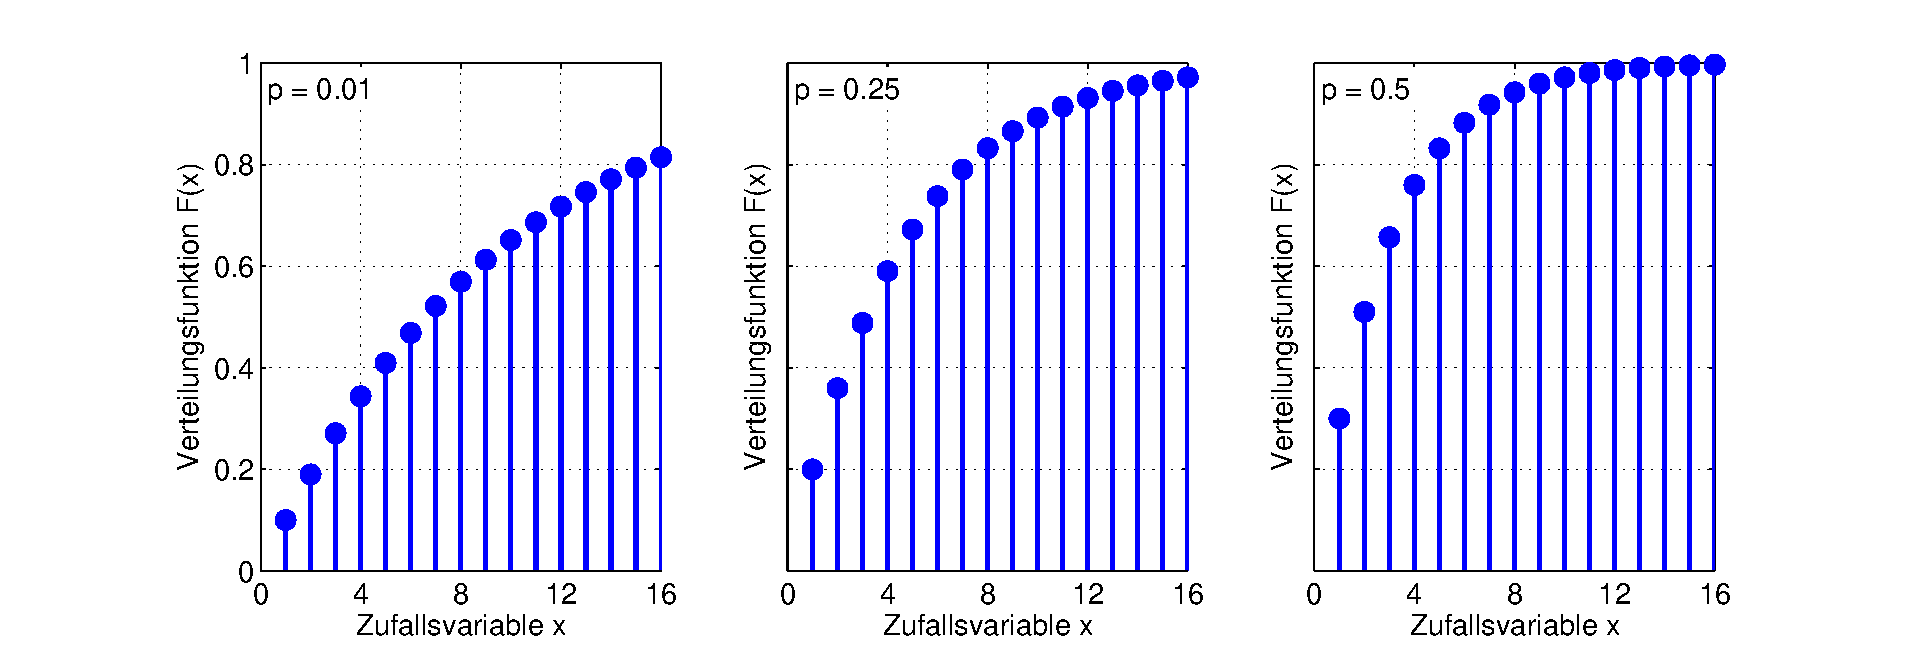
\includegraphics[width=1\textwidth]{Kapitel4/Bilder/image19}}
  \caption{Grafische Darstellung der Wahrscheinlichkeitsverteilung f(x) einer geometrischen Verteilung f\"{u}r unterschiedliche Erfolgswahrscheinlichkeiten p}
  \label{fig:Diskret_Geometrische1}
\end{figure}

\noindent Die Verteilungsfunktion F(x) ergibt sich aus der Summe von f(x). Da mindestens ein Ereignis stattfinden muss, startet die Summe bei eins.

\begin{equation}\label{eq:fourhundredfiftyeight}
F(x)=\sum _{x_{n} =1}^{x}p\cdot (1-p)^{x_{n} -1}  =\sum _{x_{n} =1}^{x}p\cdot q^{x_{n} -1}
\end{equation}

\noindent Im Fall der geometrischen Verteilung ist die Summe unendlich, da es theoretisch unendlich lange dauern kann, bis ein g\"{u}nstiges Ereignis stattfindet. Der Grenzwert von F(x) ergibt sich f\"{u}r x $\rightarrow$ $\infty$ zu

\begin{equation}\label{eq:fourhundredfiftynine}
{\mathop{\lim }\limits_{x\to \infty }} \left(F\left(x\right)\right)=\sum _{x_{n} =1}^{\infty }p\cdot q^{x_{n} -1}  =\dfrac{p}{q} \cdot \sum _{x_{n} =1}^{\infty }q^{x_{n} }  =\dfrac{p}{q} \cdot \left(\dfrac{1}{1-q} -1\right)=1
\end{equation}

\noindent Das Ergebnis entspricht dem zweiten Axiom der Wahrscheinlichkeit. Die in Bild \ref{fig:Diskret_Geometrische2} dargestellte Verteilungsfunktion F(x) f\"{u}r verschiedene Wahrscheinlichkeiten p zeigt das Verhalten nach Gleichung \eqref{eq:fourhundredfiftynine}, sie n\"{a}hert sich exponentiell der Asymptote 1 an.

\noindent 
\begin{figure}[H]
  \centerline{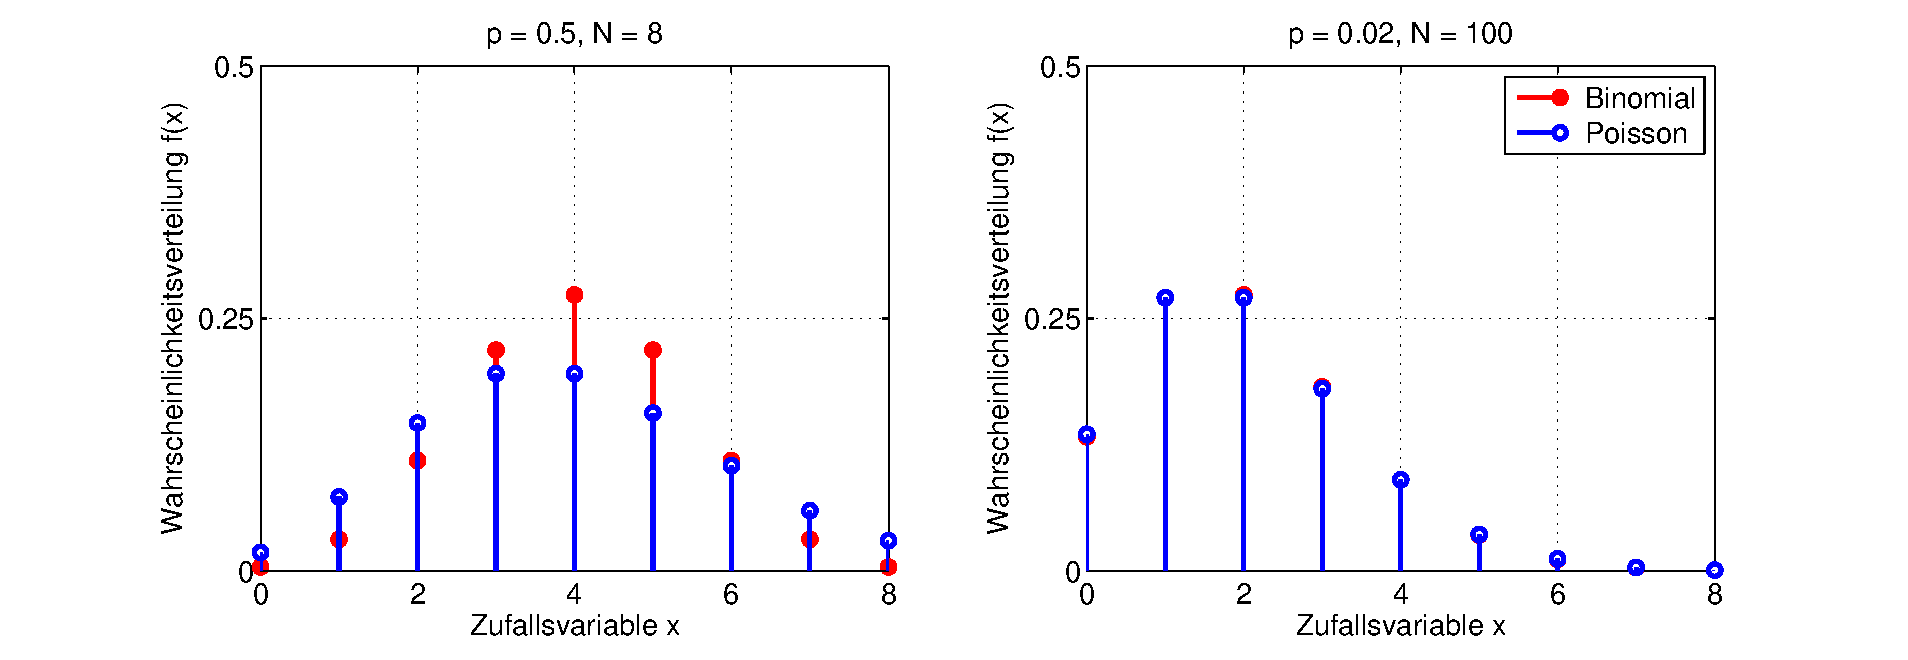
\includegraphics[width=1\textwidth]{Kapitel4/Bilder/image17}}
  \caption{Grafische Darstellung der Wahrscheinlichkeitsverteilung f(x) einer geometrischen Verteilung f\"{u}r unterschiedliche Erfolgswahrscheinlichkeiten p}
  \label{fig:Diskret_Geometrische2}
\end{figure}

\noindent Der Mittelwert der geometrischen Verteilung errechnet sich zu

\begin{equation}\label{eq:fourhundredsixty}
\mu =\sum _{x_{n} =1}^{\infty }x_{n} \cdot (1-p)^{x_{n} -1} \cdot p =\dfrac{1}{p}
\end{equation}

\noindent und die Varianz betr\"{a}gt

\begin{equation}\label{eq:fourhundredsixtyone}
\sigma ^{2} =\dfrac{1}{N-1} \cdot \sum _{n=1}^{N}\left(x_{n} -\mu \right)^{2} \cdot (1-p)^{x_{n} -1} \cdot p =\dfrac{1-p}{p^{2} }
\end{equation}

\noindent Geometrische Verteilungen werden angewendet, wenn die Wahrscheinlichkeit f\"{u}r Wartezeiten angegeben werden soll, bis zu der ein Ereignis eintritt. Ein wichtiges Anwendungsgebiet ist das Absch\"{a}tzen von Wahrscheinlichkeiten f\"{u}r Ausf\"{a}lle von Ger\"{a}ten und das Absch\"{a}tzen von Fehlerraten bei der Daten\"{u}bertragung.\bigskip

\noindent
\colorbox{lightgray}{%
\arrayrulecolor{white}%
\renewcommand\arraystretch{0.6}%
\begin{tabular}{ wl{16.5cm} }
{\fontfamily{phv}\selectfont{Beispiel: Lebensdauer eines optischen Signalgebers}}
\end{tabular}%
}\medskip 

\noindent Ein optischer Signalgeber wird in einem festen Zeitabstand eingeschaltet. Die Wahrscheinlichkeit, dass der Signalgeber beim Einschalten ausf\"{a}llt, betr\"{a}gt 0.02 \%. Die Wahrscheinlichkeit, dass der optische Signalgeber nicht w\"{a}hrend des Einschaltens ausf\"{a}llt, kann vernachl\"{a}ssigt werden. Mithilfe der geometrischen Verteilung soll die Lebensdauer als Anzahl der Einschaltzyklen des Signalgebers bestimmt werden. Bild \ref{fig:Diskret_Geometrische_LebensdauerSignalgeber} zeigt die Wahrscheinlichkeitsverteilung f(x) und die Verteilungsfunktion F(x) der Anzahl von Schaltzyklen bis zum Ausfall des optischen Signalgebers.

\clearpage

\noindent 
\begin{figure}[H]
  \centerline{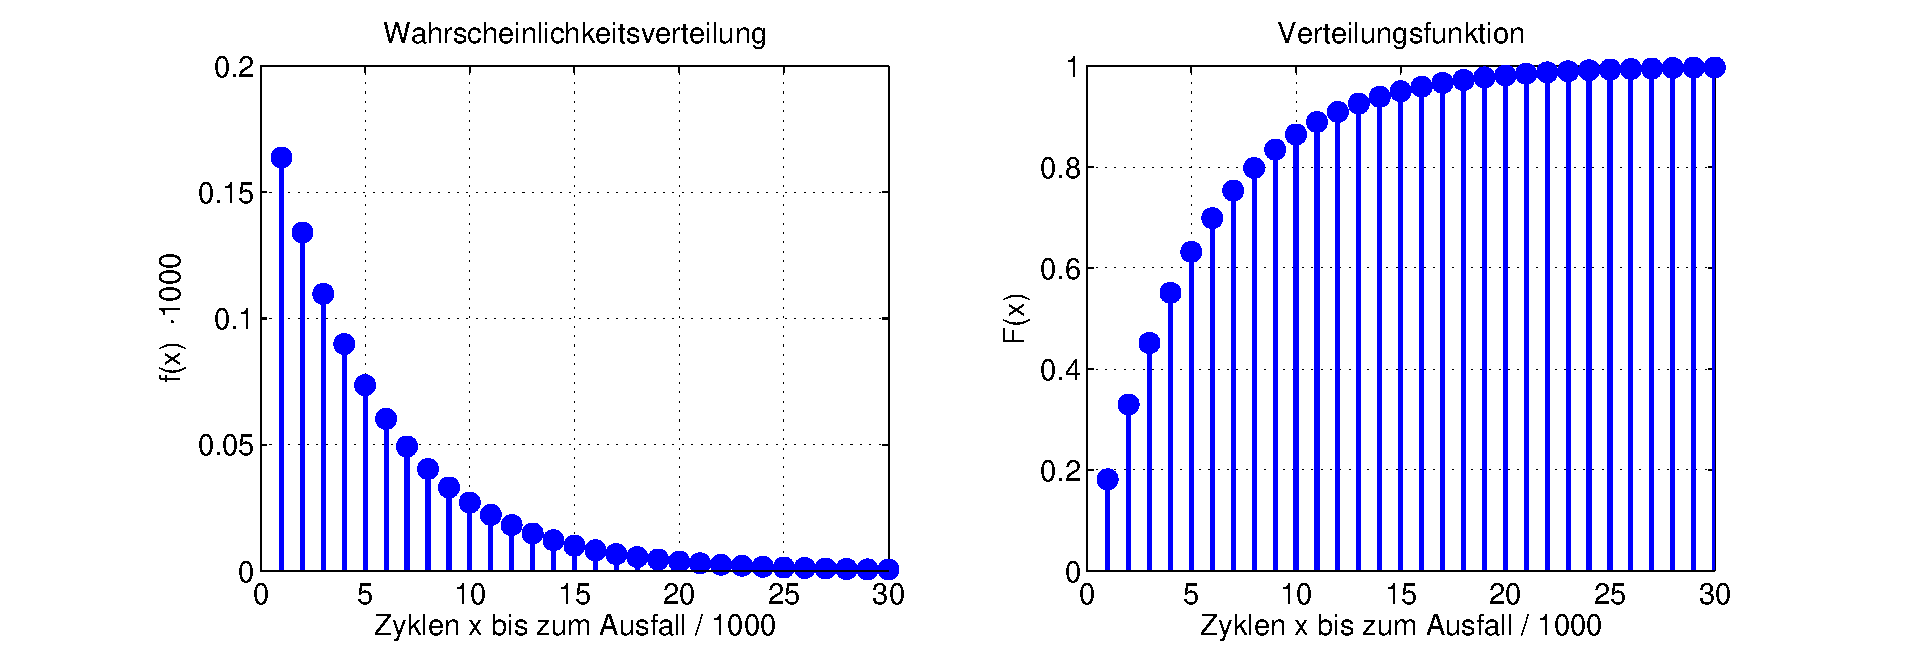
\includegraphics[width=1\textwidth]{Kapitel4/Bilder/image20}}
  \caption{Grafische Darstellung der Wahrscheinlichkeitsverteilung f(x) und Verteilungsfunktion F(x) der Anzahl von Schaltzyklen bis zum Ausfall}
  \label{fig:Diskret_Geometrische_LebensdauerSignalgeber}
\end{figure}

\noindent Der Mittelwert der geometrischen Verteilung aus Bild~4.20Bild~4.20 berechnet sich zu

\begin{equation}\label{eq:fourhundredsixtytwo}
\mu =\dfrac{1}{p} =\dfrac{1}{0.0002} =5000
\end{equation}

\noindent Die mittlere Lebensdauer des optischen Signalgebers liegt somit bei 5000 Einschaltzyklen. Die Wahrscheinlichkeit, dass der optische Signalgeber nicht mehr als 5000 Zyklen funktioniert, kann mit der Verteilungsfunktion berechnet werden zu

\begin{equation}\label{eq:fourhundredsixtythree}
F(5000)=\sum _{x=1}^{N}p\cdot (1-p)^{x-1} =\sum _{x=1}^{5000}0.0002\cdot (1-0.0002)^{x-1} =63.22\% 
\end{equation}

\noindent Die Berechnung erfolgte durch die im Folgenden dargestellte MATLAB-Sequenz.

\clearpage 


\lstinputlisting[caption = {}]{Kapitel4/mat9.m}

\noindent In Python ergibt sich folgender Programmausschnitt.

\lstinputlisting[caption = {}]{Kapitel4/mat10.m}

{\fontfamily{phv}\selectfont
\noindent\textbf{ Zusammenfassung der diskreten Verteilungen}}\smallskip

\noindent Im vorangegangenen Abschnitt werden spezielle diskrete Verteilungen vorgestellt und deren Anwendung an einem Beispiel verdeutlicht. Die Zusammenh\"{a}nge zwischen der Bernoulli, der Binomial- und der Poisson- sowie der Hypergeometrischen Verteilung sind nochmals in Bild \ref{fig:UebersichtDiskreteVerteilungen} grafisch dargestellt. 

\noindent 
\begin{figure}[H]
  \centerline{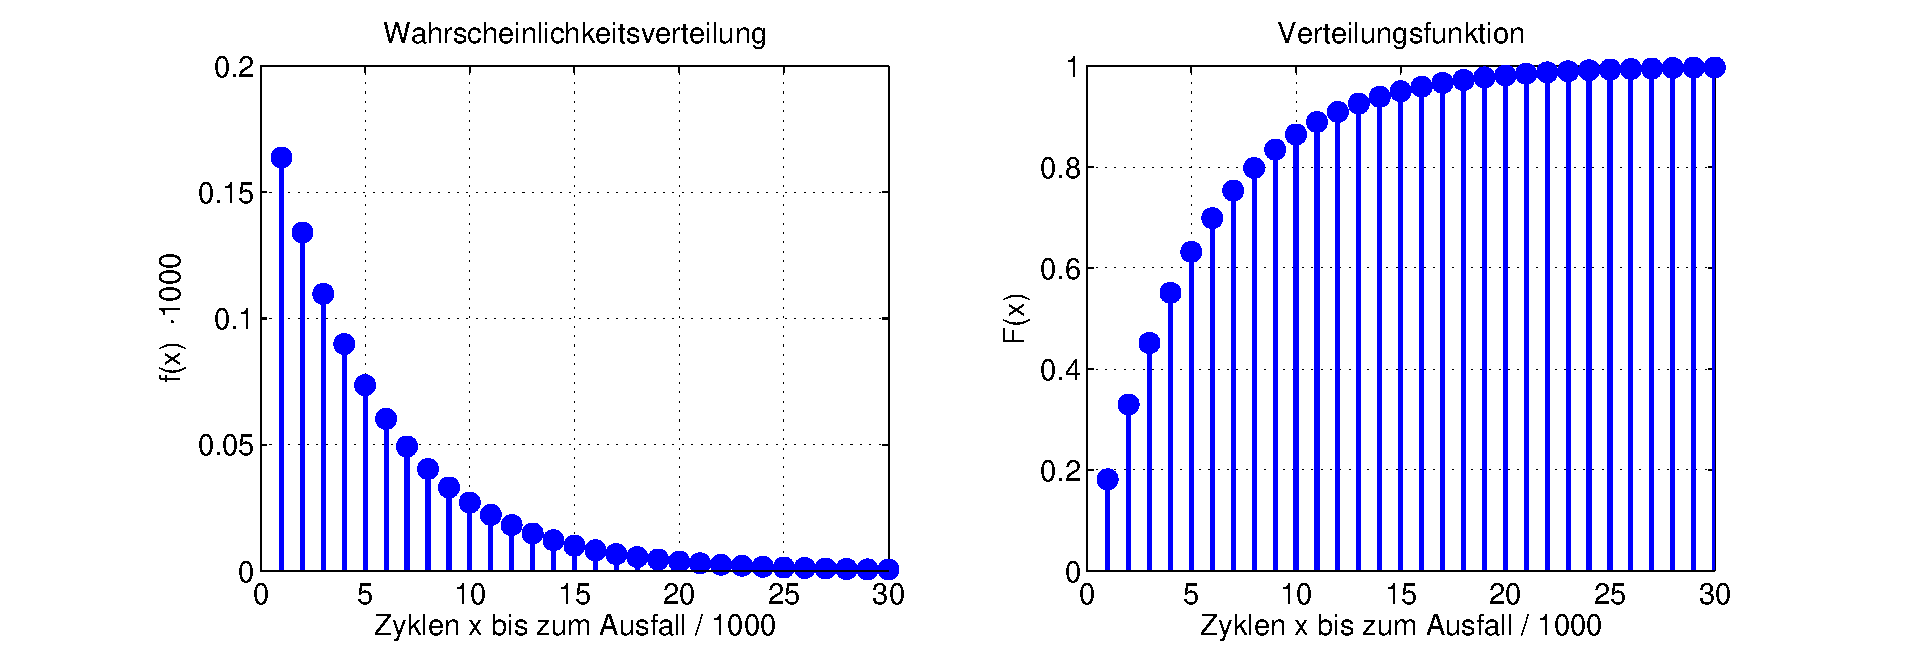
\includegraphics[width=1\textwidth]{Kapitel4/Bilder/image20}}
  \caption{Zusammenhang diskreter Verteilungen f\"{u}r die Anzahl x f\"{u}r das Eintreffen eines Ereignisses A}
  \label{fig:UebersichtDiskreteVerteilungen}
\end{figure}

\noindent Tabelle \ref{tab:foureleven} gibt eine \"{U}bersicht \"{u}ber die diskutierten diskreten Wahrscheinlichkeitsverteilungen und ihren Anwendungen. 

\clearpage
\begin{table}[H]
\setlength{\arrayrulewidth}{.1em}
\caption{\"{U}bersicht \"{u}ber diskrete Wahrscheinlichkeitsverteilungen}
\setlength{\fboxsep}{0pt}%
\colorbox{lightgray}{%
\arrayrulecolor{white}%
\begin{tabular}{| c | c | c |}
\hline
\parbox[c][0.3in][c]{1.7in}{\smallskip\centering\textbf{\fontfamily{phv}\selectfont{Name und Anwendung}}} &
\parbox[c][0.3in][c]{2.8in}{\smallskip\centering\textbf{\fontfamily{phv}\selectfont{Wahrscheinlichkeitsverteilung}}} &
\parbox[c][0.3in][c]{1.9in}{\smallskip\centering\textbf{\fontfamily{phv}\selectfont{Kenngr\"{o}{\ss}en $\mu$ und $\sigma ^{2}$}}}\\ \hline

\parbox[c][1.3in][c]{1.7in}{\centering\fontfamily{phv}\selectfont{Gleichverteilung: \newline
\\
Gleiche Wahrscheinlichkeit f\"{u}r alle Ereignisse}} & 
\parbox[c][1.3in][c]{2.8in}{\centering\fontfamily{phv}\selectfont{$f(x)=p=\dfrac{1}{N} $}} &
\parbox[c][1.3in][c]{1.9in}{\centering\fontfamily{phv}\selectfont{$\mu =\dfrac{1}{N} \cdot \sum _{n=1}^{N}x_{n} $\bigskip

$\sigma ^{2} =\dfrac{1}{N} \cdot \sum _{n=1}^{N}\left(x_{n} -\mu \right)^{2}  $}}\\
\hline

\parbox[c][1.3in][c]{1.7in}{\centering\fontfamily{phv}\selectfont{Bernoulli-Verteilung:\newline
\\
G\"{u}nstiges / ung\"{u}nstiges Ereignis bei einfacher Ausf\"{u}hrung des Experimentes}} & 
\parbox[c][1.3in][c]{2.8in}{\centering\fontfamily{phv}\selectfont{$f(x)=\left\{\begin{array}{ll} 
p  \text{ für } x=1 \\ 
q=1-p  \text{ für }   x=0  
\end{array}\right. $}} &
\parbox[c][1.3in][c]{1.9in}{\centering\fontfamily{phv}\selectfont{$\mu =p$\bigskip

$\sigma ^{2} =p\cdot q$}}\\
\hline

\parbox[c][1.3in][c]{1.7in}{\centering\fontfamily{phv}\selectfont{Binomial-Verteilung:\newline
\\
Anzahl g\"{u}nstiger Ereignisse bei N-facher Ausf\"{u}hrung, konstante Erfolgswahrscheinlichkeit}} & 
\parbox[c][1.3in][c]{2.8in}{\centering\fontfamily{phv}\selectfont{$f(x)=\left(\begin{array}{l} {N} \\ {x} \end{array}\right)\cdot p^{x} \cdot q^{N-x} $}} &
\parbox[c][1.3in][c]{1.9in}{\centering\fontfamily{phv}\selectfont{$\mu=N\cdot p $ \bigskip

$\sigma ^{2} =N\cdot p\cdot q$}}\\
\hline

\parbox[c][1.5in][c]{1.7in}{\centering\fontfamily{phv}\selectfont{Hypergeometrische Verteilung:
\newline
\\
Anzahl günstiger Ereignisse bei N-facher Ausführung, variable Erfolgswahrscheinlichkeit}} & 
\parbox[c][1.5in][c]{2.8in}{\centering\fontfamily{phv}\selectfont{$f(x)=\dfrac{\left(\begin{array}{l} {N} \\ {x} \end{array}\right)\cdot \left(\begin{array}{l} {M-G} \\ {G-x} \end{array}\right)}{\left(\begin{array}{l} {M} \\ {N} \end{array}\right)} $}} &
\parbox[c][1.5in][c]{1.9in}{\centering\fontfamily{phv}\selectfont{$\mu =N\cdot \dfrac{G}{M} $ \bigskip

$\sigma ^{2} =\dfrac{N\cdot G\cdot (M-G)\cdot (M-N)}{M^{2} \cdot (M-1)} $}}\\
\hline

\parbox[c][1.1in][c]{1.7in}{\centering\fontfamily{phv}\selectfont{Poisson-Verteilung:\newline
\\
Approximation der Binomialverteilung}} & 
\parbox[c][1.1in][c]{2.8in}{\centering\fontfamily{phv}\selectfont{$f(x)=\dfrac{\mu ^{x} }{x!} \cdot e^{-\mu } $}} &
\parbox[c][1.1in][c]{1.9in}{\centering\fontfamily{phv}\selectfont{$\mu =N\cdot p$ \bigskip

$\sigma ^{2} =N\cdot p=\mu $}}\\
\hline

\parbox[c][1.5in][c]{1.7in}{\centering\fontfamily{phv}\selectfont{Geometrische Verteilung:\newline
\\
Anzahl von Wiederholunges des Experimentes, bis das g\"{u}nstige Ereignis eintritt}} & 
\parbox[c][1.5in][c]{2.8in}{\centering\fontfamily{phv}\selectfont{$f(x)=p\cdot q^{x-1} $}} &
\parbox[c][1.5in][c]{1.9in}{\centering\fontfamily{phv}\selectfont{$\mu =\dfrac{1}{p} $ \bigskip

$\sigma ^{2} =\dfrac{1-p}{p^{2} } $}}\\
\hline

\end{tabular}%
}
\label{tab:foureleven}
\end{table}

\noindent Sowohl die Wahrscheinlichkeitsverteilung als auch die Verteilungsfunktione der in Tabelle 4.11 aufgelisteten Verteilungen sind bei MATLAB in der Statistic Toolbox implementiert. Dabei werden die folgenden Endungen f\"{u}r die MATLAB-Funktionen eingesetzt:

\begin{itemize}
    \item pdf Wahrscheinlichkeitsverteilung f(x) (probability density function)
    \item  cdf Verteilungsfunktion F(x) (cumulative distribution function)
    \item  inv Inverse Verteilungsfunktion F$^{-1}$(x) (inverse cumulative distribution function)
    \item  rnd Zufallszahlen-Generator einer Verteilung
\end{itemize}

\noindent Tabelle \ref{tab:fourtwelve} gibt eine \"{U}bersicht \"{u}ber eine Auswahl von MATLAB-Funktionen zu diskreten Verteilungen.

\clearpage 

\begin{table}[H]
\setlength{\arrayrulewidth}{.1em}
\caption{Übersicht über diskrete Wahrscheinlichkeitsverteilungen in MATLAB}
\setlength{\fboxsep}{0pt}%
\colorbox{lightgray}{%
\arrayrulecolor{white}%
\begin{tabular}{| c | c | c | c | c |}
\hline
\parbox[c][0.8in][c]{1.3in}{\smallskip\centering\textbf{\fontfamily{phv}\selectfont{Verteilung}}} &
\parbox[c][0.8in][c]{1.1in}{\smallskip\centering\textbf{\fontfamily{phv}\selectfont{Wahrscheinlich-keitsverteilung f(x)}}} &
\parbox[c][0.8in][c]{1.1in}{\smallskip\centering\textbf{\fontfamily{phv}\selectfont{Verteilungs-funktion F(x)}}} &
\parbox[c][0.8in][c]{1.1in}{\smallskip\centering\textbf{\fontfamily{phv}\selectfont{inverse Vertei-lungsfunktion F$^{-1}$(x)}}} &
\parbox[c][0.8in][c]{1.4in}{\smallskip\centering\textbf{\fontfamily{phv}\selectfont{Zufallszahlen-generator}}}\\ \hline

\parbox[c][0.5in][c]{1.3in}{\centering\fontfamily{phv}\selectfont{Gleichverteilung}} & 
\parbox[c][0.5in][c]{1.1in}{\centering\fontfamily{phv}\selectfont{unidpdf(x,N)}} &
\parbox[c][0.5in][c]{1.1in}{\centering\fontfamily{phv}\selectfont{unidcdf(x,N)}} & 
\parbox[c][0.5in][c]{1.1in}{\centering\fontfamily{phv}\selectfont{unidinv(P,N)}}  & 
\parbox[c][0.5in][c]{1.4in}{\centering\fontfamily{phv}\selectfont{unidrnd(N,m,n)}} \\
\hline

\parbox[c][0.5in][c]{1.3in}{\centering\fontfamily{phv}\selectfont{Binomial-Verteilung}} & 
\parbox[c][0.5in][c]{1.1in}{\centering\fontfamily{phv}\selectfont{binopdf(x,N,p)}} &
\parbox[c][0.5in][c]{1.1in}{\centering\fontfamily{phv}\selectfont{binocdf(x,N,p)}} & 
\parbox[c][0.5in][c]{1.1in}{\centering\fontfamily{phv}\selectfont{binoinv (Y,N,p)}}  & 
\parbox[c][0.5in][c]{1.4in}{\centering\fontfamily{phv}\selectfont{binornd(N,p,m,n)}} \\
\hline

\parbox[c][0.5in][c]{1.3in}{\centering\fontfamily{phv}\selectfont{Hypergeometrische Verteilung}} & 
\parbox[c][0.5in][c]{1.1in}{\fontfamily{phv}\selectfont{hygepdf(x,M,G,N)}} &
\parbox[c][0.5in][c]{1.1in}{\fontfamily{phv}\selectfont{hygecdf(x,M,G,N)}} & 
\parbox[c][0.5in][c]{1.1in}{\fontfamily{phv}\selectfont{hygeinv(P,M,G,N)}}  & 
\parbox[c][0.5in][c]{1.4in}{\centering\fontfamily{phv}\selectfont{hygernd(M,G,N,m,n)}} \\
\hline

\parbox[c][0.5in][c]{1.3in}{\centering\fontfamily{phv}\selectfont{Poisson-Verteilung}} & 
\parbox[c][0.5in][c]{1.1in}{\centering\fontfamily{phv}\selectfont{poisspdf(x,$\mu$)}} &
\parbox[c][0.5in][c]{1.1in}{\centering\fontfamily{phv}\selectfont{poisscdf(x,$\mu$)}} & 
\parbox[c][0.5in][c]{1.1in}{\centering\fontfamily{phv}\selectfont{poissinv(P,$\mu$)}}  & 
\parbox[c][0.5in][c]{1.4in}{\centering\fontfamily{phv}\selectfont{poissrnd($\mu$,m,n)}} \\
\hline

\parbox[c][0.5in][c]{1.3in}{\centering\fontfamily{phv}\selectfont{Geometrische Verteilung}} & 
\parbox[c][0.5in][c]{1.1in}{\centering\fontfamily{phv}\selectfont{geopdf(x,p)}} &
\parbox[c][0.5in][c]{1.1in}{\centering\fontfamily{phv}\selectfont{geocdf(x,p)}} & 
\parbox[c][0.5in][c]{1.1in}{\centering\fontfamily{phv}\selectfont{geoinv(P,p)}}  & 
\parbox[c][0.5in][c]{1.4in}{\centering\fontfamily{phv}\selectfont{geornd(p,m,n)}} \\
\hline

\end{tabular}%
}
\label{tab:fourtwelve}
\end{table}


\noindent Tabelle \ref{tab:fourthirteen} gibt eine \"{U}bersicht \"{u}ber eine Auswahl von Python-Funktionen der Bibliothek scipy.stats zu diskreten Verteilungen.

\begin{table}[H]
\setlength{\arrayrulewidth}{.1em}
\caption{\"{U}bersicht \"{u}ber diskrete Wahrscheinlichkeitsverteilungen der Python Bibliothek scipy.stats}
\setlength{\fboxsep}{0pt}%
\colorbox{lightgray}{%
\arrayrulecolor{white}%
\begin{tabular}{| c | c | c | c | c |}
\hline
\parbox[c][0.8in][c]{1.3in}{\smallskip\centering\textbf{\fontfamily{phv}\selectfont{Verteilung}}} &
\parbox[c][0.8in][c]{1.1in}{\smallskip\centering\textbf{\fontfamily{phv}\selectfont{Wahrscheinlich-keitsverteilung f(x)}}} &
\parbox[c][0.8in][c]{1.1in}{\smallskip\centering\textbf{\fontfamily{phv}\selectfont{Verteilungs-funktion F(x)}}} &
\parbox[c][0.8in][c]{1.1in}{\smallskip\centering\textbf{\fontfamily{phv}\selectfont{inverse Vertei-lungsfunktion F$^{-1}$(x)}}} &
\parbox[c][0.8in][c]{1.4in}{\smallskip\centering\textbf{\fontfamily{phv}\selectfont{Zufallszahlen-generator}}}\\ \hline

\parbox[c][0.5in][c]{1.3in}{\centering\fontfamily{phv}\selectfont{Gleichverteilung}} & 
\parbox[c][0.5in][c]{1.1in}{\centering\fontfamily{phv}\selectfont{randint.pmf}} &
\parbox[c][0.5in][c]{1.1in}{\centering\fontfamily{phv}\selectfont{randint.cdf}} & 
\parbox[c][0.5in][c]{1.1in}{\centering\fontfamily{phv}\selectfont{randint.ppf}}  & 
\parbox[c][0.5in][c]{1.4in}{\centering\fontfamily{phv}\selectfont{randint.rvs}} \\
\hline

\parbox[c][0.5in][c]{1.3in}{\centering\fontfamily{phv}\selectfont{Binomial-Verteilung}} & 
\parbox[c][0.5in][c]{1.1in}{\centering\fontfamily{phv}\selectfont{binom.pmf}} &
\parbox[c][0.5in][c]{1.1in}{\centering\fontfamily{phv}\selectfont{binom.cdf}} & 
\parbox[c][0.5in][c]{1.1in}{\centering\fontfamily{phv}\selectfont{binom.ppf}}  & 
\parbox[c][0.5in][c]{1.4in}{\centering\fontfamily{phv}\selectfont{binom.rvs}} \\
\hline

\parbox[c][0.5in][c]{1.3in}{\centering\fontfamily{phv}\selectfont{Hypergeometrische Verteilung}} & 
\parbox[c][0.5in][c]{1.1in}{\centering\fontfamily{phv}\selectfont{hypergeom.pmf}} &
\parbox[c][0.5in][c]{1.1in}{\centering\fontfamily{phv}\selectfont{hypergeom.cdf}} & 
\parbox[c][0.5in][c]{1.1in}{\centering\fontfamily{phv}\selectfont{hypergeom.ppf}}  & 
\parbox[c][0.5in][c]{1.4in}{\centering\fontfamily{phv}\selectfont{hypergeom.rvs}} \\
\hline

\parbox[c][0.5in][c]{1.3in}{\centering\fontfamily{phv}\selectfont{Poisson-Verteilung}} & 
\parbox[c][0.5in][c]{1.1in}{\centering\fontfamily{phv}\selectfont{poisson.pmf}} &
\parbox[c][0.5in][c]{1.1in}{\centering\fontfamily{phv}\selectfont{poisson.cdf}} & 
\parbox[c][0.5in][c]{1.1in}{\centering\fontfamily{phv}\selectfont{poisson.ppf}}  & 
\parbox[c][0.5in][c]{1.4in}{\centering\fontfamily{phv}\selectfont{poisson.rvs}} \\
\hline

\parbox[c][0.5in][c]{1.3in}{\centering\fontfamily{phv}\selectfont{Geometrische Verteilung}} & 
\parbox[c][0.5in][c]{1.1in}{\centering\fontfamily{phv}\selectfont{geom.pmf}} &
\parbox[c][0.5in][c]{1.1in}{\centering\fontfamily{phv}\selectfont{geom.cdf}} & 
\parbox[c][0.5in][c]{1.1in}{\centering\fontfamily{phv}\selectfont{geom.ppf}}  & 
\parbox[c][0.5in][c]{1.4in}{\centering\fontfamily{phv}\selectfont{geom.rvs}} \\
\hline

\end{tabular}%
}
\label{tab:fourthirteen}
\end{table}

\clearpage 

\subsection{Spezielle stetige Verteilungen}

\noindent Die Beschreibung stetiger Zufallsgr\"{o}{\ss}en erfolgt durch stetige Verteilungen. Dazu sind in den folgenden Abschnitten spezielle stetige Verteilungen aufgef\"{u}hrt. Einen besonderen Status nehmen Test- oder Pr\"{u}fverteilungen ein, denen der Abschnitt 4.7 gewidmet ist.

\subsubsection{Gleichverteilung}

\noindent Analog zu den diskreten Verteilungen wird als einfachstes Beispiel die Gleichverteilung definiert. Sie weist in einem Intervall von a bis b eine konstante Wahrscheinlichkeitsdichte f(x) = k f$_{0}$ auf, au{\ss}erhalb dieses Intervalls ist die Wahrscheinlichkeitsdichte null. Die Wahrscheinlichkeit f\"{u}r das sichere Ereignis ist

\begin{equation}\label{eq:fourhundredsixtyfour}
F(\infty )=\int _{-\infty }^{\infty }f(x)dx =f_{0} \cdot (b-a)=1
\end{equation}

\noindent Damit ergibt sich f\"{u}r die Wahrscheinlichkeitsdichte f(x) 

\begin{equation}\label{eq:fourhundredsixtyfive}
f(x)=\left\{\begin{array}{l} {\dfrac{1}{b-a} \text{für} < x\le  b} \\ 
{0 \text{ für alle übrigen Werte} } \end{array}\right.
\end{equation}

\noindent Durch Integration ergibt sich eine Verteilungsfunktion von 

\begin{equation}\label{eq:fourhundredsixtysix}
F(x)=\int _{a}^{x}\dfrac{1}{b-a} d\xi  =\dfrac{x-a}{b-a} \text{für} a < x \le b
\end{equation}

\noindent Bild \ref{fig:Stetig_Gleichverteilung} stellt die Wahrscheinlichkeitsdichte f(x) und Verteilungsfunktion F(x) einer stetigen Gleichverteilung dar.

\begin{figure}[H]
  \centerline{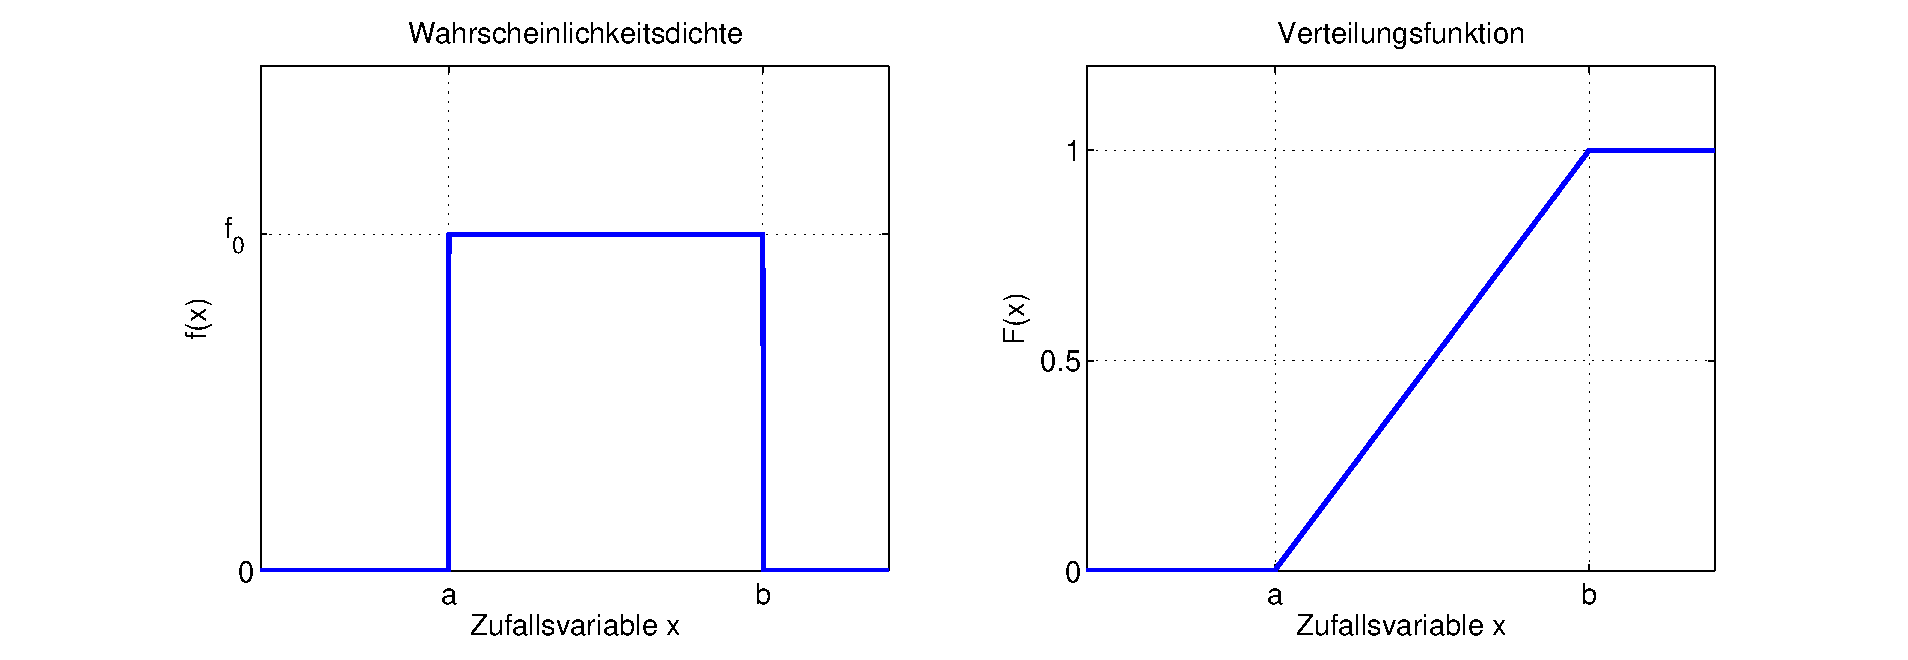
\includegraphics[width=1\textwidth]{Kapitel4/Bilder/image22}}
  \caption{Grafische Darstellung der Wahrscheinlichkeitsdichte f(x) und der Verteilungsfunktion F(x) f\"{u}r eine Gleichverteilung}
  \label{fig:Stetig_Gleichverteilung}
\end{figure}

\noindent Der Mittelwert einer Gleichverteilung ergibt sich zu

\begin{equation}\label{eq:fourhundredsixtyseven}
\mu =E(x)=\int _{-\infty}^{\infty}x\cdot f(x) dx=\int _{a}^{b}x\cdot \dfrac{1}{b-a} dx=\dfrac{b^{2} -a^{2} }{2\cdot (b-a)} =\dfrac{a+b}{2}
\end{equation}

\clearpage 

\noindent Die Varianz einer Gleichverteilung berechnet sich zu

\begin{equation}\label{eq:fourhundredsixtyeight}
\sigma _{}^{2} =E\left((x-\mu)^{2} \right)=E\left(x^{2} \right)-E^{2} \left(x\right)=\dfrac{b^{3} -a^{3} }{3\cdot \left(b-a\right)} -\dfrac{(a+b)^{2} }{4} =\dfrac{(b-a)^{2} }{12}
\end{equation}

\noindent Typische Anwendungsgebiete sind die Berechnung von durchschnittlichen Wartezeiten bei Transportprozessen oder Bedienungssystemen sowie die statistische Beschreibung von Diskretisierungsvorg\"{a}ngen. 

\noindent
\colorbox{lightgray}{%
\arrayrulecolor{white}%
\renewcommand\arraystretch{0.6}%
\begin{tabular}{ wl{16.5cm} }
{\fontfamily{phv}\selectfont
\noindent
Beispiel: Effektivwert des Quantisierungsrauschens eines A/D-Wandlers}
\end{tabular}%
}\bigskip

\noindent Um ein analoges Eingangssignal U$_{E}$ in ein digitales Ausgangssignal U$_{ADC}$ zu wandeln, wird das zeitkontinuierliche Signal quantisiert. Die Quantisierung in diskrete Amplitudenwerte erfolgt dabei durch einen Analog-Digital-Wandler mit einer Aufl\"{o}sung von N~Bit. Durch die damit festgelegte, endliche Anzahl von 2$^{N}$ Quantisierungsstufen entsteht ein Fehler, der als Quantisierungsrauschen q aufgefasst werden kann. Bild \ref{fig:GleichverteilungADC}3 zeigt zwei Quantisierungsstufen und einen Eingangsspannungswert U$_{E}$.

\noindent 

\begin{figure}[H]
  \centerline{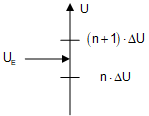
\includegraphics[width=0.3\textwidth]{Kapitel4/Bilder/image23}}
  \caption{Quantisierung eines Eingangssignals U$_{E}$ durch einen Analog-Digital-Wandler}
  \label{fig:GleichverteilungADC}
\end{figure}

\noindent Die H\"{o}he einer Quantisierungsstufe $\Delta$U wird bei einem Analog-Digital-Wandler durch die Anzahl der Quantisierungsstufen und den Messbereich U$_{MAX}$ zu 

\begin{equation}\label{eq:fourhundredsixtynine}
\Delta U=\dfrac{U_{MAX} }{2^{N}}
\end{equation}

\noindent definiert. Der Signalwert U$_{E}$ wird durch den Analog-Digital-Wandler entweder auf den Wert n$.\Delta$U oder auf den Wert (n + 1)$.\Delta$U quantisiert. Dadurch ist der Fehler q in dem Intervall - $\Delta$U/2 $\mathrm{\le}$ q $\mathrm{\le}$ $\Delta$U/2 gleichverteilt mit der Wahrscheinlichkeitsdichte

\begin{equation}\label{eq:fourhundredseventy}
f_{0} =\dfrac{1}{\Delta U}
\end{equation}

\noindent Zur Bewertung des Fehlers wird oft der Effektivwert des Quantisierungsrauschens herangezogen. Der Effektivwert einer Zufallsgr\"{o}{\ss}e ist allgemein als die Wurzel aus dem Erwartungswert des Quadrates der Zufallszahl definiert. F\"{u}r das Quantisierungsrauschen folgt mit den Rechenregeln zum Erwartungswert

\begin{equation}\label{eq:fourhundredseventyone}
q_{EFF}^{2} =E\left(q^{2} \right)=\sigma _{q}^{2} +E\left(q\right)^{2} =\sigma _{q}^{2} +\mu _{q}^{2}
\end{equation}

\noindent F\"{u}r die Gleichverteilung des Quantisierungsrauschens berechnet sich der Mittelwert zu

\begin{equation}\label{eq:fourhundredseventytwo}
\mu _{q} =\dfrac{1}{2} \cdot \left(\dfrac{-\Delta U}{2} +\dfrac{\Delta U}{2} \right)=0
\end{equation}

\noindent Die Varianz folgt zu

\begin{equation}\label{eq:fourhundredseventythree}
\sigma _{q}^{2} =\dfrac{1}{12} \cdot \left(\dfrac{\Delta U}{2} -\dfrac{-\Delta U}{2} \right)^{2} =\dfrac{\Delta U^{2} }{12}
\end{equation}

\noindent Damit ergibt sich der Effektivwert des Quantisierungsrauschens eines Analog-Digital-Wandlers zu

\begin{equation}\label{eq:fourhundredseventyfour}
q_{EFF} =\sqrt{\sigma _{q}^{2} } =\dfrac{\Delta U}{\sqrt{12} } \approx \dfrac{\Delta U}{3.46}
\end{equation}

\noindent Der Effektivwert des Quantisierungsrauschens eines Analog-Digital-Wandlers kann damit aus den technischen Daten ermittelt werden.

\subsubsection{Dreiecksverteilung}

\noindent Liegen nur sehr wenige konkrete Daten zur Bestimmung der Verteilungsfunktion f(x) einer Zufallsvariablen x vor, wird in der Praxis die Dreiecksverteilung als erste Sch\"{a}tzung verwendet. Die Dreiecksverteilung ist auch als Simpson-Verteilung bekannt. Ihre Wahrscheinlichkeitsverteilung ist in dem Intervall a $\mathrm{<}$ x $\leq$ b definiert durch

\begin{equation}\label{eq:fourhundredseventyfive}
f(x)=\left\{\begin{array}{l} {\dfrac{2}{(b-a)\cdot (c-a)} \cdot (x-a)\text{ für }a<{\rm x}\le c} \\ 
{\dfrac{2}{(b-a)\cdot (b-c)} \cdot (b-x)\text{ für }c< x\le b} \end{array}\right.
\end{equation}

Au{\ss}erhalb des Intervalls a $\mathrm{<}$ x $\leq$ b ist die Wahrscheinlichkeit null. In Gleichung \eqref{eq:fourhundredseventyfive} beschreibt der Parameter a den kleinsten und der Parameter b den gr\"{o}{\ss}ten Wert der Zufallsvariablen x, der Parameter c gibt die Lage des Maximums an. Durch Integration ergibt sich die Verteilungsfunktion F(x) aus Gleichung \eqref{eq:fourhundredseventyfive} zu

\begin{equation}\label{eq:fourhundredseventysix}
F(x)=\left\{\begin{array}{l} {\dfrac{(x-a)^{2} }{(b-a)\cdot (c-a)}\text{ für }< x\le c} \\ 
{1-\dfrac{(b-x)^{2} }{(b-a)\cdot (b-c)}\text{ für }c < x\le b} \end{array}\right.
\end{equation}

Bild \ref{fig:Stetig_Dreiecksverteilung} stellt die Wahrscheinlichkeitsdichte f(x) und Verteilungsfunktion F(x) dar.

\begin{figure}[H]
  \centerline{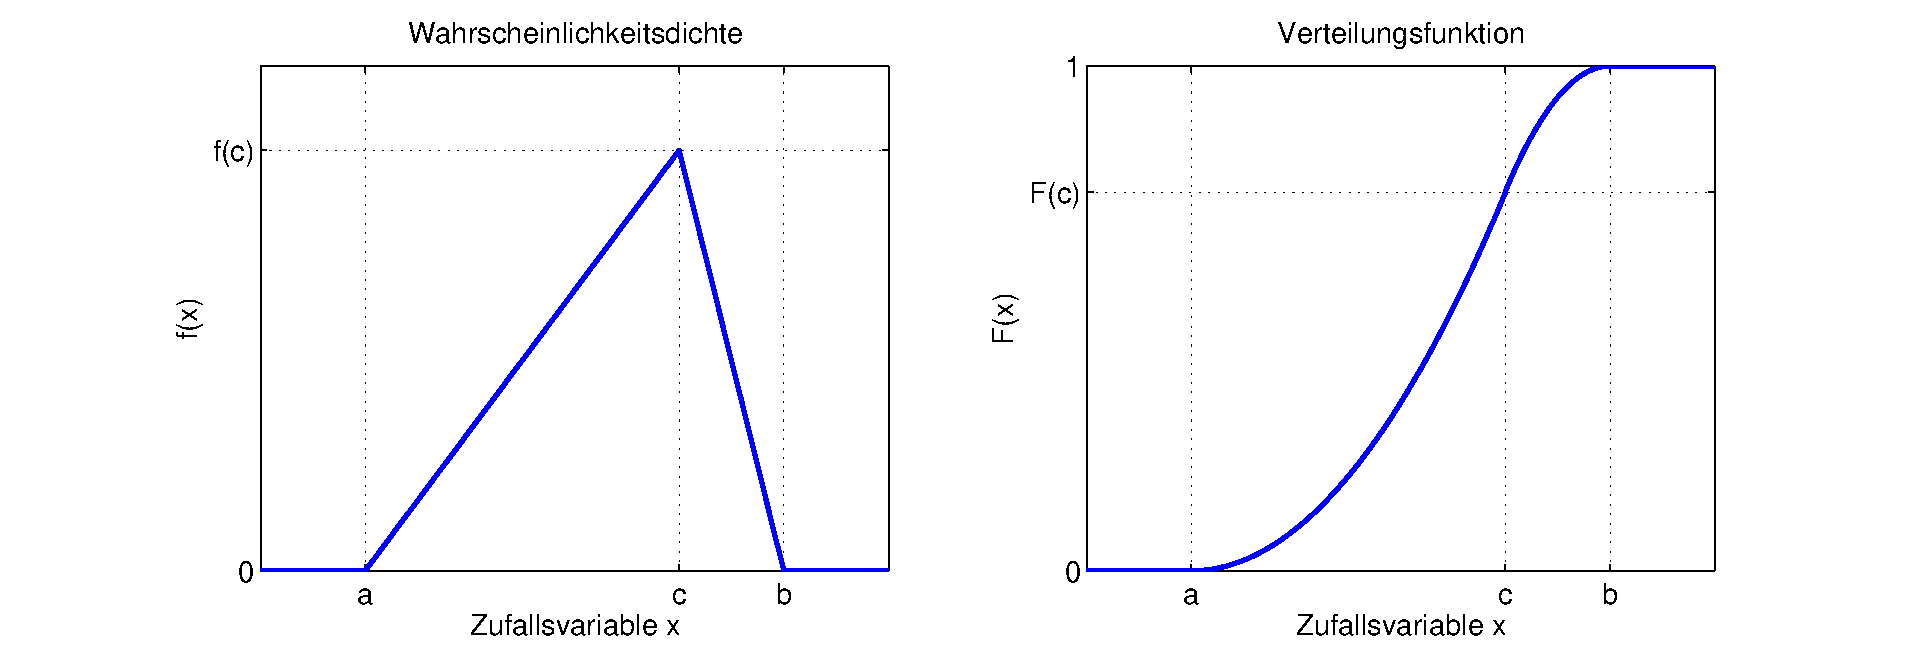
\includegraphics[width=1\textwidth]{Kapitel4/Bilder/image24}}
  \caption{Wahrscheinlichkeitsdichte f(x) und Verteilungsfunktion F(x) f\"{u}r eine stetige Dreiecksverteilung}
  \label{fig:Stetig_Dreiecksverteilung}
\end{figure}

\noindent An der Stelle c besitzt die Wahrscheinlichkeitsverteilung f(x) ihr Maximum, das sich aus

\begin{equation}\label{eq:fourhundredseventyseven}
F(\infty)=\int _{-\infty}^{\infty}f(x)dx =\dfrac{b-a}{2} \cdot f(c)=1
\end{equation}

\noindent ergibt zu

\begin{equation}\label{eq:fourhundredseventyeight}
f(c)=\dfrac{2}{b-a}
\end{equation}

\noindent Die Wahrscheinlichkeit P(x $\mathrm{\le}$ c) berechnet sich zu

\begin{equation}\label{eq:fourhundredseventynine}
P\left(x\le c\right)=F(c)=\int _{-\infty }^{x}f(\xi )d\xi  =\dfrac{1}{2} \cdot (c-a)\cdot \dfrac{2}{b-a} =\dfrac{c-a}{b-a}
\end{equation}

\noindent Der Mittelwert der durch Gleichung \eqref{eq:fourhundredseventyfive} definierten stetigen Dreiecksverteilung liegt bei

\begin{equation}\label{eq:fourhundredseighty}
\mu =E(x)=\dfrac{a+b+c}{3}
\end{equation}

\noindent Die Varianz der dreiecksverteilten Zufallsvariable x ergibt sich aus

\begin{equation}\label{eq:fourhundredseightyone}
\sigma ^{2} =E\left(x^{2} \right)-\mu ^{2} =\dfrac{a^{2} +b^{2} +c^{2} -a\cdot b-a\cdot c-b\cdot c}{18} =\dfrac{(a-b)^{2} +(b-c)^{2} +(a-c)^{2} }{36}
\end{equation}

\noindent Bei Fragestellungen, bei denen keine detaillierten Daten vorliegen und die Annahme einer Gleichverteilung nicht gerechtfertigt ist, wird meist eine Drei-Punkt-Sch\"{a}tzung mithilfe der Dreiecksverteilung durchgef\"{u}hrt. Derartige Sch\"{a}tzungen werden unter anderen zur Berechnung des ben\"{o}tigten Budgets oder zur Bestimmung eines Auslieferungsdatums an Endkunden bei der Projektplanung ben\"{o}tigt. Dabei werden Parameter a, b und c aus der Erfahrung heraus bestimmt.\bigskip

\noindent
\colorbox{lightgray}{%
\arrayrulecolor{white}%
\renewcommand\arraystretch{0.6}%
\begin{tabular}{ wl{16.5cm} }
{\fontfamily{phv}\selectfont
\noindent
Beispiel: Drei-Punkt-Sch\"{a}tzung eines Projektaufwandes}
\end{tabular}%
}\bigskip

\noindent Das Vorgehen einer Drei-Punkt-Sch\"{a}tzung wird an einem Beispiel zur Planung der Zeitdauer f\"{u}r die Programmierung einer Software verdeutlicht. Der Software-Entwickler sch\"{a}tzt, dass er f\"{u}r die Programmierung einer derartigen Software durchschnittlich 60 Stunden ben\"{o}tigt. Im g\"{u}nstigsten Fall sch\"{a}tzt er eine Bearbeitungsdauer von 45 Stunden, treten Probleme bei der Hardware auf, kann sich der Aufwand auf 150 Stunden vergr\"{o}{\ss}ern.

\noindent Es ergibt sich damit die in Bild \ref{fig:Stetig_Dreiecksverteilung_Projektaufwand} gesch\"{a}tzte Dreiecksverteilung mit einem Maximum von

\begin{equation}\label{eq:fourhundredseightytwo}
f(c)=\dfrac{2}{b-a} =\dfrac{2}{150-45} =0.019
\end{equation}

\noindent an der Stelle c = 60 Stunden.

\begin{figure}[H]
  \centerline{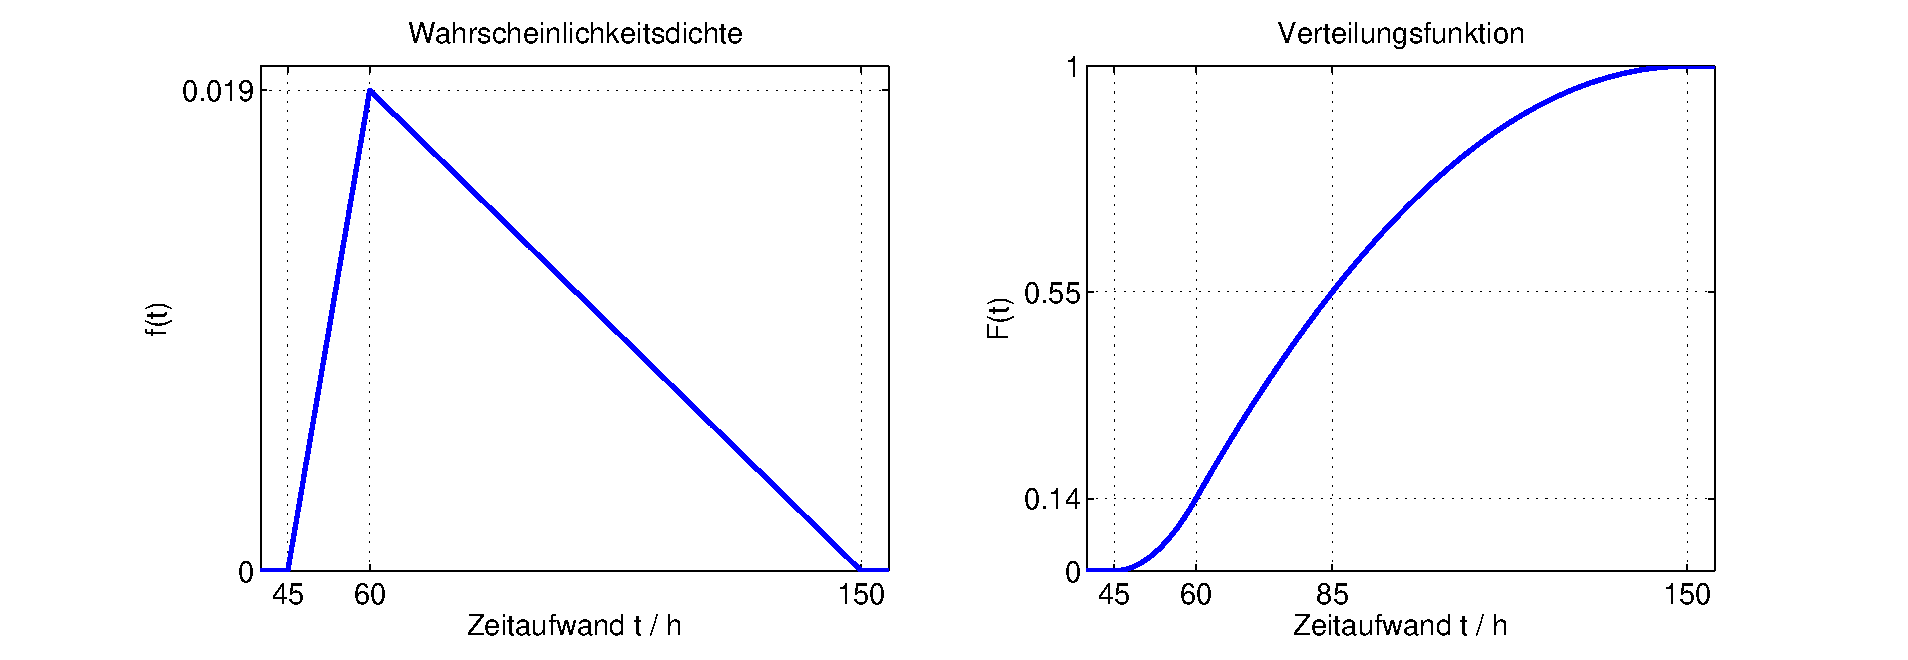
\includegraphics[width=1\textwidth]{Kapitel4/Bilder/image25}}
  \caption{Grafische Darstellung der gesch\"{a}tzten Verteilung des Projektaufwandes}
  \label{fig:Stetig_Dreiecksverteilung_Projektaufwand}
\end{figure}


\noindent Der mittlere Aufwand f\"{u}r das Projekt berechnet sich mit Gleichung \eqref{eq:fourhundredseighty} zu

\begin{equation}\label{eq:fourhundredseightythree}
\mu =\dfrac{a+b+c}{3} =\dfrac{45+60+150}{3} h=85 h
\end{equation}

\noindent Aus der Wurzel der in Gleichung \eqref{eq:fourhundredseightyone} definierten Varianz folgt die Standardabweichung der Verteilung zu

\begin{equation}\label{eq:fourhundredseightyfour}
\sigma =\sqrt{\dfrac{(a-b)^{2} +(b-c)^{2} +(a-c)^{2} }{36}} =\sqrt{\dfrac{(45-150)^{2} +(150-60)^{2} +(45-60)^{2} }{36}} h= 23.18 h
\end{equation}

\noindent Die mittlere Sch\"{a}tzung des Programmierers von 60 Stunden wird lediglich mit einer Wahrscheinlichkeit von 

\begin{equation}\label{eq:fourhundredseightyfive}
F(x=c)=\dfrac{c-a}{b-a} =\dfrac{60-45}{150-45} =14.29 \%
\end{equation}

\noindent erreicht. Daher wird zum Beispiel zur Absch\"{a}tzung der Kosten, die durch das Projekt entstehen, der mittlere Zeitaufwand von 85 Stunden herangezogen. Dieser wird bei der vorliegenden gesch\"{a}tzten Verteilung mit einer Wahrscheinlichkeit von 55.29 \% eingehalten.

\subsubsection{Weibull-Verteilung}

\noindent Die Weibull-Verteilung wird unter anderem zur Modellierung von Lebensdauern in der Qualit\"{a}tssicherung verwendet. Sie wird vor allem bei Fragestellungen wie der Materialerm\"{u}dung von spr\"{o}den Werkstoffen oder dem Ausfallen von elektronischen Bauteilen eingesetzt. Benannt ist sie nach dem Schweden Waloddi Weibull. Die Wahrscheinlichkeitsdichte der Weibull-Verteilung ist f\"{u}r x $\mathrm{<}$ 0 null. F\"{u}r x $\geq$ 0 ist sie definiert als

\begin{equation}\label{eq:fourhundredseightysix}
f(x)=\left\{\begin{array}{c} {\dfrac{\beta }{\eta } \cdot \left(\dfrac{x}{\eta } \right)^{\beta -1} \cdot e^{-\left(\dfrac{x}{\eta } \right)^{\beta } } \text{ für } x\ge 0} \\ 
{0 \qquad \text{ für } x<0} \end{array}\right.
\end{equation}

\noindent Die Verteilungsfunktion F(x) der Weibull-Verteilung lautet 

\begin{equation}\label{eq:fourhundredseightyseven}
F(x)=1-e^{-\left(\dfrac{x}{\eta } \right)^{\beta}}
\end{equation}

\noindent Der Parameter $\beta$ beschreibt, ob die Ausfallrate \"{u}ber der Lebensdauer zunimmt ($\beta$ $\mathrm{>}$ 1), abnimmt (0~$\mathrm{<}$~$\beta$~$\mathrm{<}$~1) oder konstant bleibt ($\beta$ = 1). Bild \ref{fig:Stetig_Weibull1} stellt die Wahrscheinlichkeitsdichte f(x) der Weibull-Verteilung f\"{u}r unterschiedliche Parametervarianten dar.

\begin{figure}[H]
  \centerline{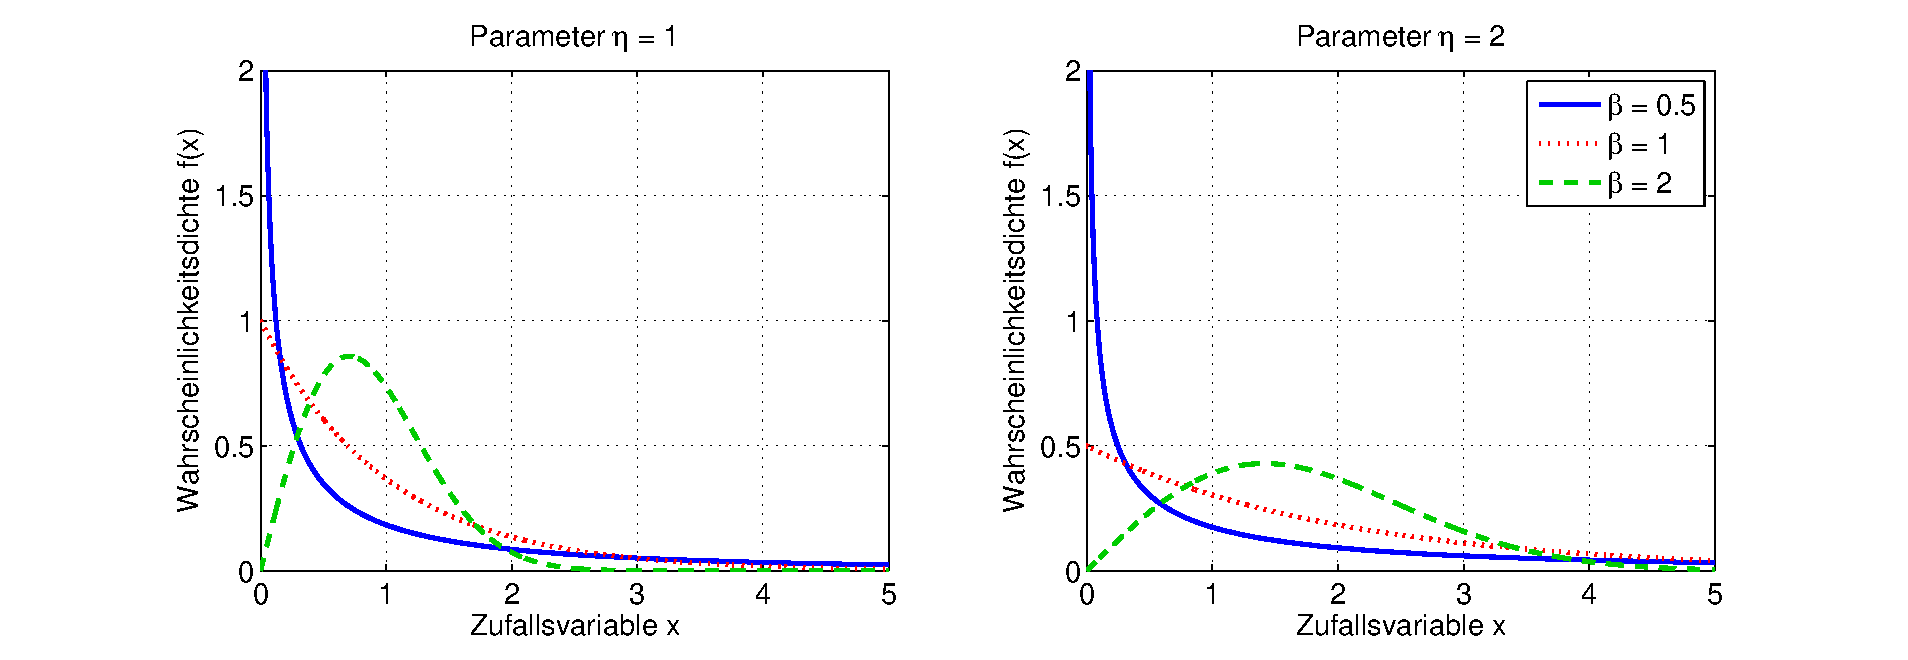
\includegraphics[width=1\textwidth]{Kapitel4/Bilder/image26}}
  \caption{Wahrscheinlichkeitsdichte f(x) der Weibullverteilung f\"{u}r $\beta$ = 0.5, 1 und 2 und $\etaup$ = 1, 2}
  \label{fig:Stetig_Weibull1}
\end{figure}

\noindent Mit wachsendem $\beta$ geht die Dichtefunktion f(x) der Weibull-Verteilung von einer rechtsschiefen in eine linksschiefe Verteilung \"{u}ber. Das entspricht der anschaulichen Vorstellung der variablen Ausfallrate. F\"{u}r kleine Werte von $\beta$ $\mathrm{<}$ 1 nimmt die Ausfallrate ab, die Verteilung wird deshalb mit wachsendem Wert der Zufallsvariablen x flacher. Mit einem Wert $\beta$ $\mathrm{>}$ 1 nimmt die Ausfallrate mit wachsendem Wert der Zufallsvariablen x zu.\newline 

\noindent Der Parameter $\etaup$ beschreibt die Lage der Verteilung auf der x-Achse. Wird mit F(x) die Verteilung von Lebensdauern beschrieben, stellt der Parameter $\etaup$ die charakteristische Lebensdauer dar. Daraus ergibt sich die Folgerung, dass $\etaup$ $\mathrm{>}$ 0 sein muss. In Anlehnung an die Zeitkonstante dynamischer \"{U}bertragungsglieder entspricht der Parameter $\etaup$ einer Lebensdauer mit einer Ausfallwahrscheinlichkeit von 63.2 \%. Zur Analyse der Bedeutung des Parameters $\etaup$ stellt Bild \ref{fig:Stetig_Weibull2} die Verteilungsfunktion F(x) f\"{u}r unterschiedliche Parameter $\beta$ und $\etaup$ dar.

\begin{figure}[H]
  \centerline{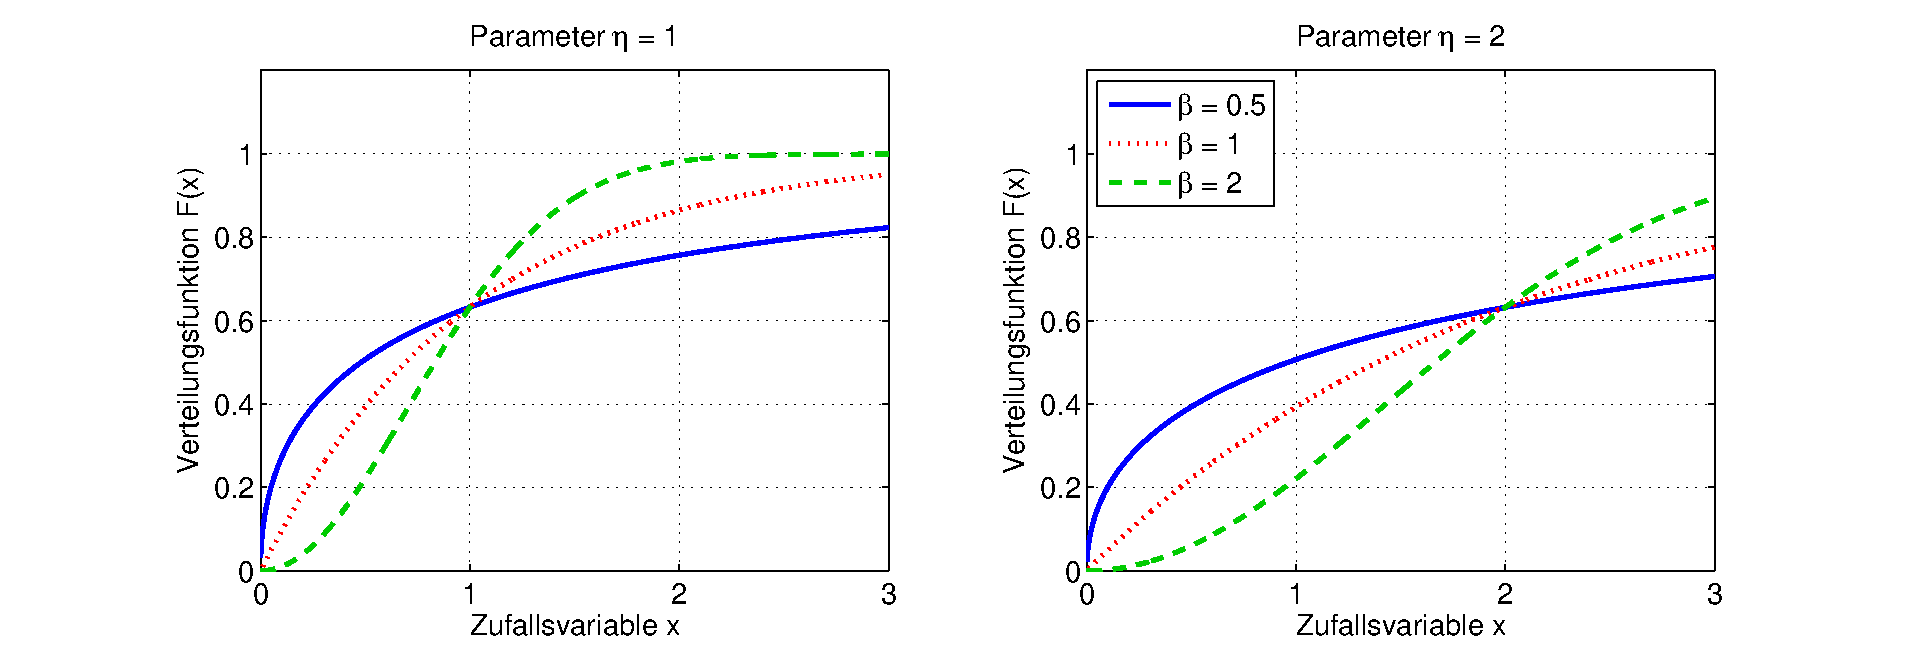
\includegraphics[width=1\textwidth]{Kapitel4/Bilder/image27}}
  \caption{Verteilungsfunktion F(x) der Weibullverteilung f\"{u}r Parameter $\beta$ = 0.5, 1 und 2 und Parameter $\etaup$ = 1, 2 }
  \label{fig:Stetig_Weibull2}
\end{figure}

\clearpage

\noindent Der Mittelwert ergibt sich zu

\begin{equation}\label{eq:fourhundredseightyeight}
\mu =\left(\dfrac{1}{\eta } \right)^{-\dfrac{1}{\beta } } \cdot \Gamma \left(\dfrac{1}{\beta } +1\right)
\end{equation}

\noindent und die Varianz berechnet sich zu

\begin{equation}\label{eq:fourhundredseightynine}
\sigma ^{2} =\left(\dfrac{1}{\eta } \right)^{-\dfrac{2}{\beta } } \cdot \left(\Gamma \left(\dfrac{2}{\beta } +1\right)-\Gamma ^{2} \left(\dfrac{1}{\beta } +1\right)\right)
\end{equation}

\noindent wobei die Funktion 

\begin{equation}\label{eq:fourhundredsninety}
\Gamma \left(\alpha \right)=\int _{0}^{\infty }e^{-u} \cdot u^{\alpha -1} du
\end{equation}

\noindent als Gamma-Funktion [Krey91] bezeichnet wird.\newline

\noindent In der Praxis ist die Weibull-Verteilung neben der Exponential-Verteilung die am h\"{a}ufigsten verwendete Lebensdauerverteilung. Dabei wird die in Bild \ref{fig:Stetig_Weibull3} gezeigte Darstellung im doppelt logarithmischen Ma{\ss}stab eingesetzt, wodurch eine Approximation der Verteilung \"{u}ber zwei Geraden erm\"{o}glicht wird. 

\begin{figure}[H]
  \centerline{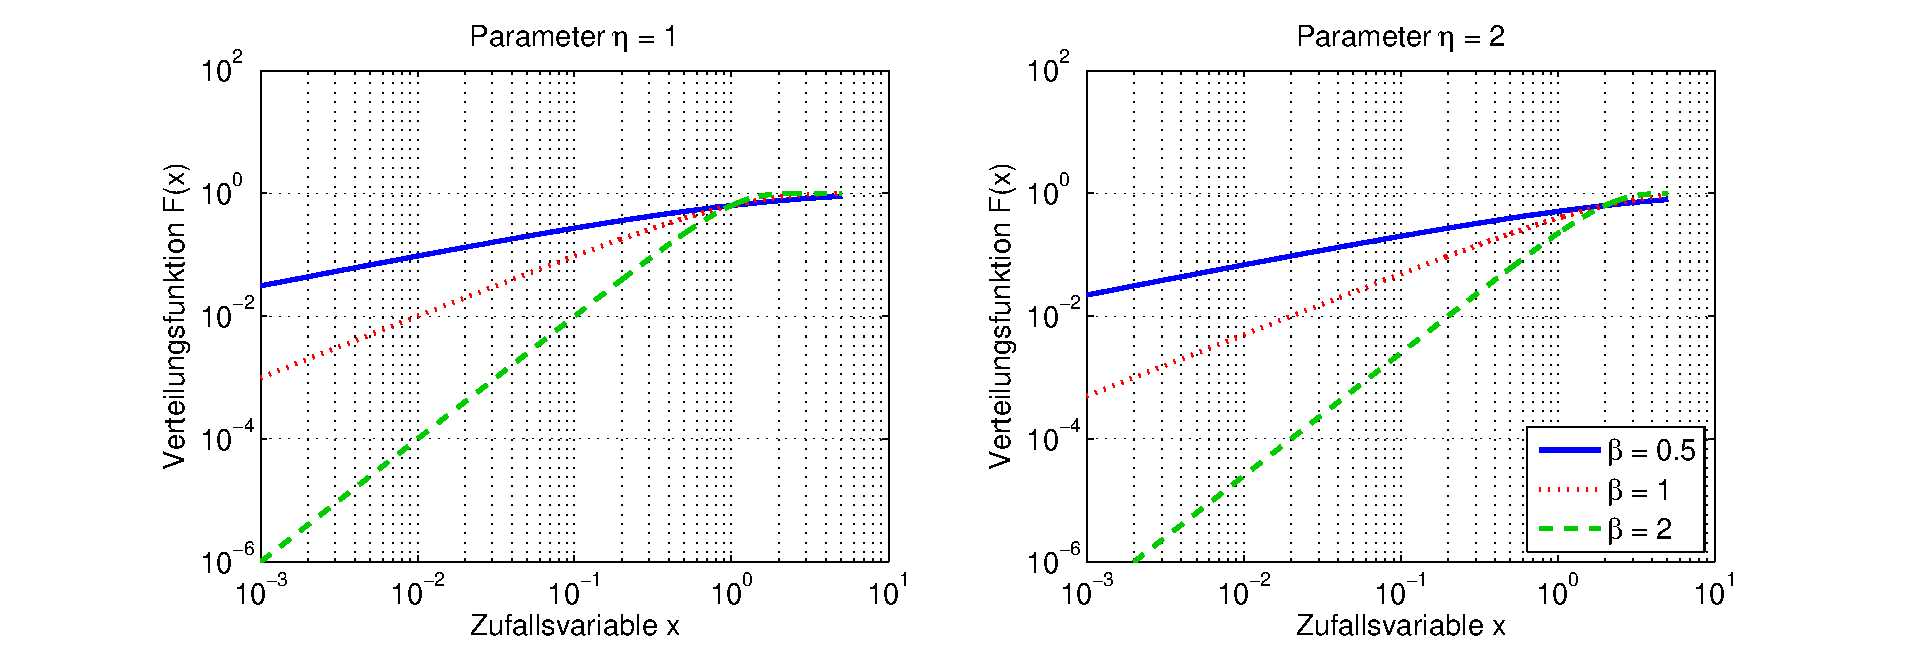
\includegraphics[width=1\textwidth]{Kapitel4/Bilder/image28}}
  \caption{Verteilungsfunktion F(x) der Weibullverteilung f\"{u}r $\beta$ = 0.5, 1 und 2 und $\etaup$ = 1, 2 im doppelt logarithmischen Ma{\ss}stab}
  \label{fig:Stetig_Weibull3}
\end{figure}

\noindent
\colorbox{lightgray}{%
\arrayrulecolor{white}%
\renewcommand\arraystretch{0.6}%
\begin{tabular}{ wl{16.5cm} }
{\fontfamily{phv}\selectfont
\noindent
Beispiel: Verteilung von Windgeschwindigkeiten}
\end{tabular}%
}\bigskip

\noindent Statt der Anwendung zur Beschreibung von Lebensdauern wird hier ein Beispiel zur Berechnung von mittleren Leistungen bei Windkraftanlagen aufgegriffen. Der nat\"{u}rliche Wind schwankt in seiner Geschwindigkeit. Um die Energieerzeugung durch eine Windkraftanlage vorhersagen zu k\"{o}nnen, muss daher bekannt sein, welche H\"{a}ufigkeitsverteilung der Wind an einem Standort besitzt. \"{U}blicherweise werden die zeitlichen H\"{a}ufigkeiten der verschiedenen Geschwindigkeiten durch die zweiparametrische Weibull-Verteilung mit den Parametern $\beta$ und $\eta$ beschrieben. 

\begin{equation}\label{eq:fourhundredsninetyone}
f(x)=\dfrac{\beta }{\eta} \cdot \left(\dfrac{x}{\eta } \right)^{\beta -1} \cdot e^{-\left(\dfrac{x}{\eta} \right)^{\beta}}
\end{equation}

\noindent Der Parameter $\beta$ ist der Weibull-Formfaktor und gibt die Form der Verteilung an, er nimmt einen Wert von $\beta$ = 1 bis 3 an. Einen gro{\ss}en $\beta$-Wert gibt es f\"{u}r Winde mit geringen Schwankungen, wie zum Beispiel bei konstanten Passatwinden. In Europa ist ein $\beta$-Faktor von 2 \"{u}blich. Sehr variable Winde, wie zum Beispiel die Winde im Polargebiet werden durch ein kleines $\beta$ beschrieben. Der Parameter $\beta$ nimmt mit der H\"{o}he leicht zu, da Turbulenzen und Schwankungen mit der H\"{o}he sinken. \newline

\noindent Der Parameter $\eta$ ist der Weibull-Skalierungsfaktor in m/s. Er steht in einem bestimmten Verh\"{a}ltnis zum Mittelwert der Windgeschwindigkeit v der Verteilung und ist damit von dem Standort der Windkraftanlage abh\"{a}ngig. Der Parameter $\etaup$ beschreibt damit die Lage der Verteilung auf der Geschwindigkeitsachse.\newline

\noindent Bild \ref{fig:Stetig_WeibullVerteilungWind} vergleicht die Windgeschwindigkeitsverteilung von Europa ($\beta$ = 2) mit der Windverteilung von Passatwinden ($\beta$ = 3) f\"{u}r einen konstanten Skalierungsfaktor von $\eta$ = 10.

\begin{figure}[H]
  \centerline{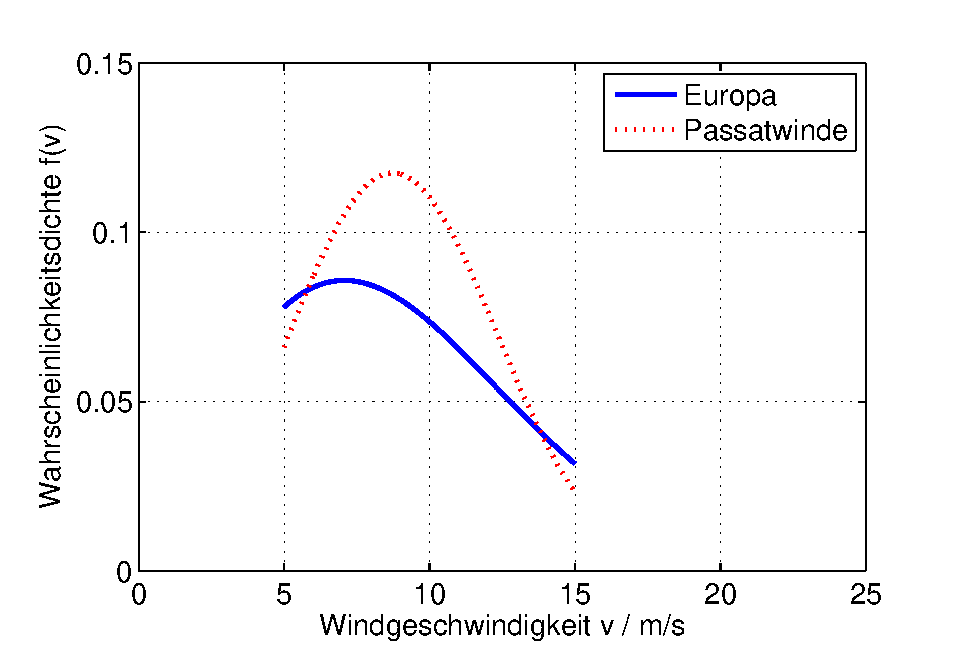
\includegraphics[width=0.5\textwidth]{Kapitel4/Bilder/image29}}
  \caption{Vergleich der Windgeschwindigkeitsverteilungen von Europa ($\beta$ = 2) mit der Windverteilung von Passatwinden ($\beta$ = 3) jeweils f\"{u}r einen Skalierungsfaktor $\eta$ = 10}
  \label{fig:Stetig_WeibullVerteilungWind}
\end{figure}


\noindent Windkraftanlagen arbeiten in einem definierten Geschwindigkeitsintervall. Bei diesem Beispiel wird eine Windkraftanlage zugrunde gelegt, die bei Geschwindigkeiten zwischen 5 und 15 m/s arbeitet, einen Rotorradius von 5 m und einen als konstant angenommenen Leistungsbeiwert c${}_{p}$ = 0.48 besitzt. Die mittlere Leistung P der Windkraftanlage errechnet sich nach mit einer Dichte und $\rho$ = 1.2 kg/m³ aus dem Erwartungswert

\begin{equation}\label{eq:fourhundredsninetytwo}
E(P)=\int _{5}^{15}c_{p} \cdot \rho \cdot A\cdot \dfrac{1}{2} \cdot v^{3} \cdot f(v) dv
\end{equation}

\noindent Dabei werden f\"{u}r f(v) je nach Standort unterschiedliche Weibull-Verteilungen zugrunde gelegt. F\"{u}r das Beispiel ergibt sich bei einem Standort in Europa ein Erwartungswert von 15.4 kW, bei einem Standort mit Passatwinden ein Erwartungswert von 19.1 kW. Aufgrund der engeren Verteilung bei Passatwinden befindet sich die Windkraftanlage oft in dem Betriebsbereich. Mit steigendem Wert $\beta$ steigt deshalb die Ausbeute der Windenergie. 

\clearpage

\noindent Die zur Berechnung erforderliche MATLAB-Sequenz zeigt sich wie folgt.

\lstinputlisting[caption = {}]{Kapitel4/mat11.m}

\noindent Die Realisierung in Python f\"{u}hrt zu demselben Ergebnis.

\lstinputlisting[caption = {}]{Kapitel4/mat12.m}

\noindent Die Weibull-Verteilung geht f\"{u}r eine konstante Ausfallrate ($\beta$ = 2) in die Rayleigh-Verteilung \"{u}ber, bei der sich der Koeffizient b errechnet aus 

\begin{equation}\label{eq:fourhundredsninetythree}
b=\dfrac{\eta }{\sqrt{2}}
\end{equation}

\noindent Die Rayleigh-Verteilung wird in Abschnitt 4.6.5 eingef\"{u}hrt und diskutiert.\newline

\noindent Ein weiterer Sonderfall der Weibull-Verteilung stellt die Exponential-Verteilung dar. Sie ergibt sich aus der Weibull-Verteilung f\"{u}r eine konstante Ausfallrate ($\beta$ = 1). Der Koeffizient $\lambda$ der Exponential-Verteilung berechnet sich aus den Parametern der Weibull-Verteilung zu

\begin{equation}\label{eq:fourhundredsninetyfour}
\lambda =\dfrac{1}{\eta }
\end{equation}

Die Exponential-Verteilung wird im folgenden Abschnitt 4.6.4 eingef\"{u}hrt.


\subsubsection{Exponential-Verteilung}

\noindent In Abschnitt 4.5.6 wird die geometrische Verteilung als Modell zur Absch\"{a}tzung von Lebensdauern und Wartezeiten abgeleitet. Dabei war die Zufallsvariable x diskret. Die entsprechende Verteilung f\"{u}r stetige Zufallsvariablen ist die Exponential-Verteilung. Sie wird angewendet, um zum Beispiel die Lebensdauer von Produkten oder Zeitr\"{a}ume bis zu Schadensf\"{a}llen zu berechnen. Voraussetzung f\"{u}r die Anwendung der Exponential-Verteilung ist, dass die noch zu erwartende Lebensdauer nicht von der bereits absolvierten Lebensdauer abh\"{a}ngig ist. Anschaulich bedeutet das, dass das Produkt keine Alterungserscheinungen aufweist. Diese Voraussetzung entspricht der Forderung nach statistischer Unabh\"{a}ngigkeit der Erfolgswahrscheinlichkeit bei der geometrischen Verteilung. \newline

\noindent Die Exponential-Verteilung ist f\"{u}r x $\mathrm{>}$ 0 definiert als 

\begin{equation}\label{eq:fourhundredsninetyfive}
f(x)=\lambda \cdot e^{-\lambda \cdot x}
\end{equation}

\noindent Daraus folgt f\"{u}r x $\mathrm{>}$ 0 die Verteilungsfunktion F(x)

\begin{equation}\label{eq:fourhundredsninetysix}
F(x)=1-e^{-\lambda \cdot x}
\end{equation}

\noindent Der Parameter $\lambda$ beschreibt, wie schnell sich die Wahrscheinlichkeitsdichte dem Wert null n\"{a}hert. Bild \ref{fig:Stetig_Exponential} stellt f\"{u}r unterschiedliche Parameter $\lambda$ die Wahrscheinlichkeitsdichte f(x) und Verteilungsfunktion F(x) der Exponential-Verteilung dar.

\begin{figure}[H]
  \centerline{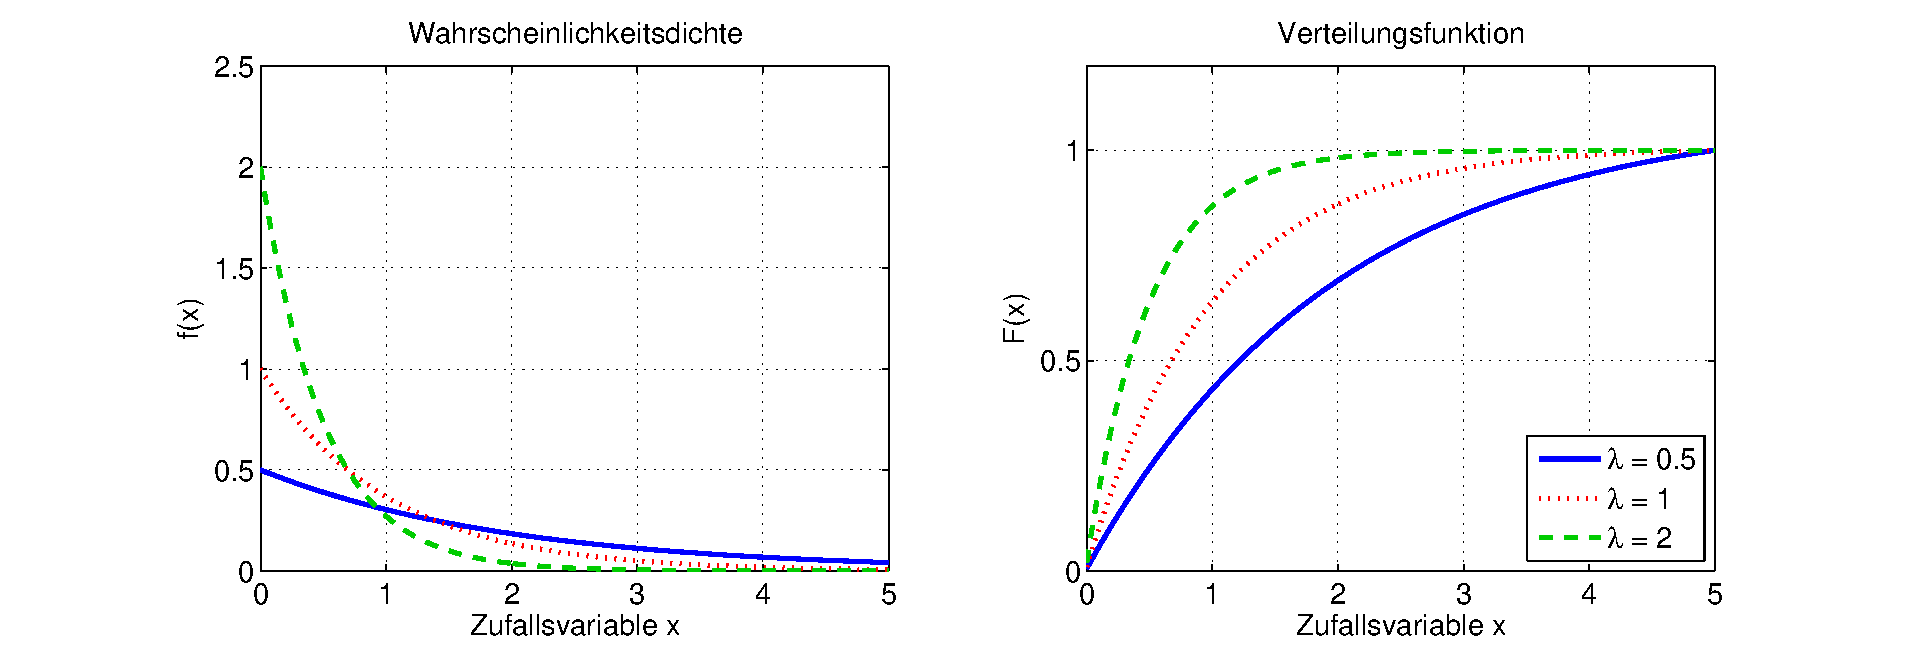
\includegraphics[width=1\textwidth]{Kapitel4/Bilder/image30}}
  \caption{Wahrscheinlichkeitsdichte f(x) und Verteilungsfunktion F(x) der Exponentialverteilung f\"{u}r $\lambda$ = 0.5, 1, 2}
  \label{fig:Stetig_Exponential}
\end{figure}

\noindent Die Erwartungswerte Mittelwert und Standardabweichung k\"{o}nnen wegen der Exponentialfunktion nicht mehr elementar bestimmt werden. Es kann gezeigt werden, dass sich der Mittelwert und die Varianz der Exponential-Verteilung berechnen zu

\begin{equation}\label{eq:fourhundredsninetyseven}
\mu =E(x)=\dfrac{1}{\lambda }
\end{equation}

\noindent und 

\begin{equation}\label{eq:fourhundredsninetyeight}
\sigma _{}^{2} =E\left(\left(x-\mu \right)^{2} \right)=E\left(x^{2} \right)-E^{2} (x)=\dfrac{1}{\lambda ^{2} }
\end{equation}

\noindent Die Exponentialfunktion wird neben der Berechnung der noch zu erwartenden Lebensdauer von Bauelementen auch f\"{u}r die Absch\"{a}tzung der mittleren Betriebsdauer zwischen Ausf\"{a}llen von Produkten oder Einrichtungen, der Mean Time Between Failures (MTBF), verwendet. Dies wird im folgenden Beispiel aufgezeigt und diskutiert.\bigskip

\noindent
\colorbox{lightgray}{%
\arrayrulecolor{white}%
\renewcommand\arraystretch{0.6}%
\begin{tabular}{ wl{16.5cm} }
{\fontfamily{phv}\selectfont
\noindent
Beispiel: Mean Time Between Failures (MTBF) eines Lasersystems}
\end{tabular}%
}\bigskip

\noindent Unter dem Begriff MTBF wird die mittlere Betriebsdauer zwischen zwei Ausf\"{a}llen einer Einheit verstanden. Die Betriebsdauer gibt dabei an, wie lange eine instandgesetzte Einheit zwischen zwei aufeinanderfolgenden Ausf\"{a}llen funktionsf\"{a}hig ist. Die mittlere Betriebsdauer kann daher als Ma{\ss} f\"{u}r die Zuverl\"{a}ssigkeit herangezogen werden und dient zur Absch\"{a}tzung von Ausf\"{a}llen in bestimmten Zeitintervallen. Ist die Betriebsdauer unter Ber\"{u}cksichtigung der oben genannten Einschr\"{a}nkungen exponentialverteilt, ergibt sich die MTBF aus dem Kehrwert der konstanten Ausfallrate $\lambda$.

\begin{equation}\label{eq:fourhundredsninetynine}
MTBF=\dfrac{1}{\lambda }
\end{equation}

\noindent F\"{u}r ein Lasersystem, dessen erreichbare mittlere Betriebsdauer von dem Hersteller mit 20 Monaten angegeben wird, ergibt sich die in Bild \ref{fig:Stetig_Exponential_MTBF} dargestellte Exponential-Verteilung mit $\lambda$ = 0.05.

\begin{figure}[H]
  \centerline{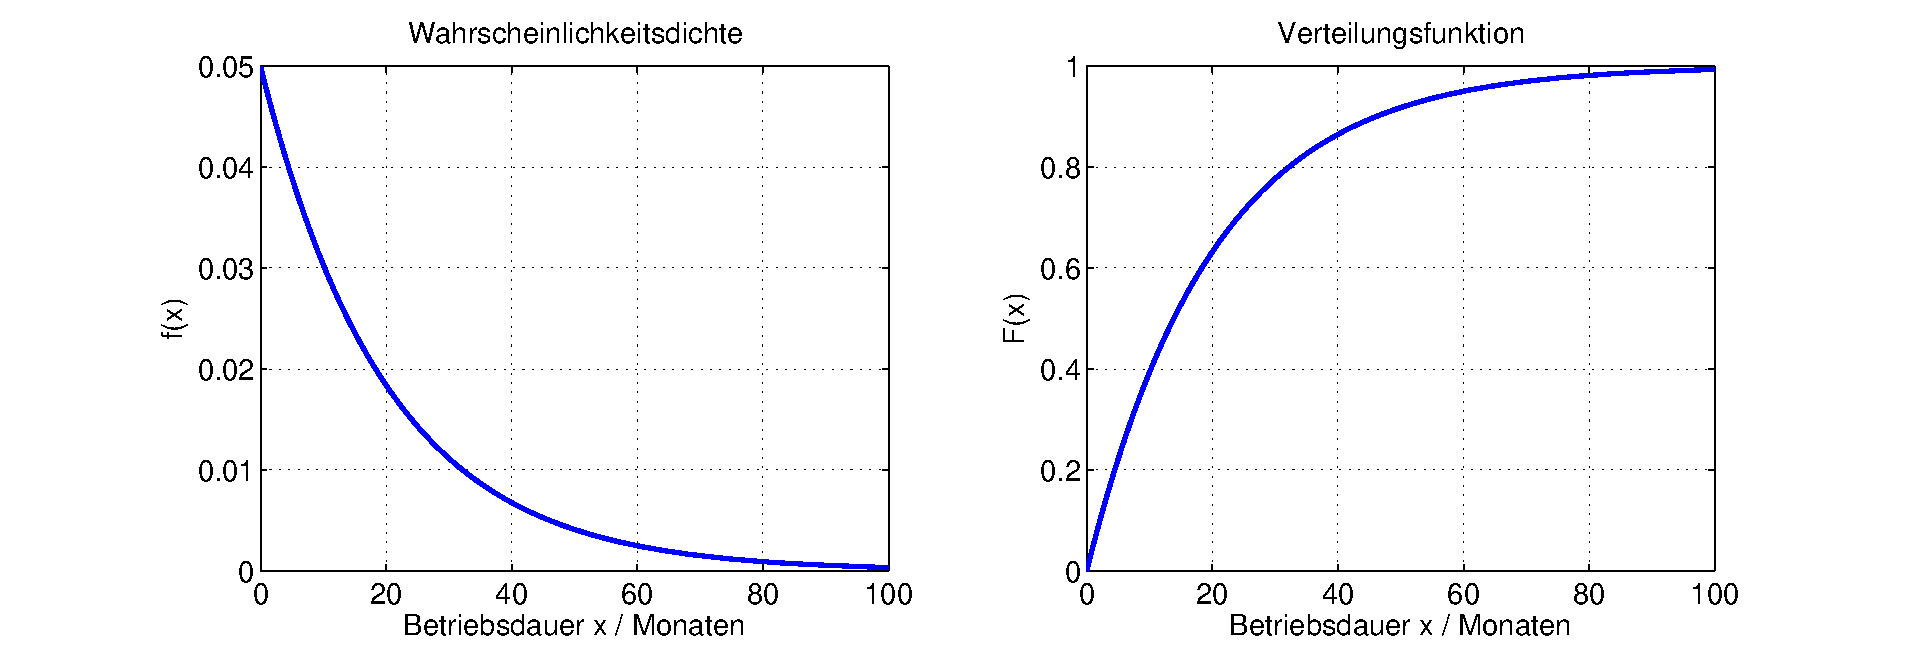
\includegraphics[width=1\textwidth]{Kapitel4/Bilder/image31}}
  \caption{Wahrscheinlichkeitsdichte f(x) und Verteilungsfunktion F(x) eines Lasersystems}
  \label{fig:Stetig_Exponential_MTBF}
\end{figure}

\noindent Bei der Interpretation des MTBF-Wertes des Lasersystems muss beachtet werden, dass der MTBF-Wert nicht aussagt, dass das Lasersystem im Mittel 20 Monate ohne Ausfall arbeitet. Aus der Verteilungsfunktion F(x) aus Bild \ref{fig:Stetig_Exponential_MTBF} berechnet sich die Wahrscheinlichkeit daf\"{u}r, dass das Lasersystem bis zur prognostizierten mittleren Betriebsdauer ausf\"{a}llt zu

\begin{equation}\label{eq:fourtwohundred}
F(MTBF)=1-e^{-0.05\cdot 20} =0.6321
\end{equation}

\noindent Lediglich 36.79 \% der Lasersysteme wird somit 20 Monate zwischen zwei Ausf\"{a}llen funktionieren. Eine vorbeugende Instandsetzung sollte daher stets vor der prognostizierten mittleren Betriebsdauer durchgef\"{u}hrt werden.\newline

\noindent Die zur Berechnung erforderliche In MATLAB- ergibt sich folgende Programm-Sequenz zeigt sich wie folgtzur Berechnung.

\lstinputlisting[caption = {}]{Kapitel4/mat13.m}

\noindent Entsprechend ergibt sich in Python.

\lstinputlisting[caption = {}]{Kapitel4/mat14.m}

\subsubsection{Rayleigh-Verteilung (Betragsverteilung 2. Art)}

\noindent Mithilfe der Rayleigh-Verteilung wird die Verteilung des Betrages zweier unabh\"{a}ngiger normalverteilter Zufallsgr\"{o}{\ss}en mit der Standardabweichung $\sigma$ = b beschrieben. Zum Beispiel folgt der Wert des Radius eines Kreises, dessen x- und y-Koordinaten normalverteilt sind, einer Rayleigh-Verteilung. Ein anderer Anwendungsfall ist die Beschreibung der 10-Minuten-Mittelwerte von Windgeschwindigkeiten. Da die Rayleigh-Verteilung die Verteilung von Betr\"{a}gen beschreibt, wird sie auch als Betragsverteilung 2. Art bezeichnet. Sie wird zur Bewertung der Prozesssicherheit im Rahmen der statistischen Prozesskontrolle eingesetzt.

\clearpage 

\noindent Die Wahrscheinlichkeitsdichte f(x) der Rayleigh-Verteilung ist definiert als

\begin{equation}\label{eq:fourtwohundredone}
f(x)=\dfrac{1}{b^{2}} \cdot x\cdot e^{-\dfrac{1}{2} \cdot \dfrac{x^{2}}{b^{2}}}
\end{equation}

\noindent Daraus ergibt sich die Verteilungsfunktion F(x) zu

\begin{equation}\label{eq:fourtwohundredtwo}
F(x)=\dfrac{1}{b^{2} } \cdot \int _{-\infty }^{x}\xi \cdot e^{-\dfrac{1}{2} \cdot \dfrac{\xi ^{2} }{b^{2}}} d\xi  =1-e^{-\dfrac{1}{2} \cdot \dfrac{x^{2} }{b^{2}}}
\end{equation}

\noindent Bild \ref{fig:Stetig_Rayleigh} zeigt die Wahrscheinlichkeitsdichte f(x) und die Verteilungsfunktion F(x) der Rayleigh-Verteilung f\"{u}r verschiedene Werte des Parameters b.

\begin{figure}[H]
  \centerline{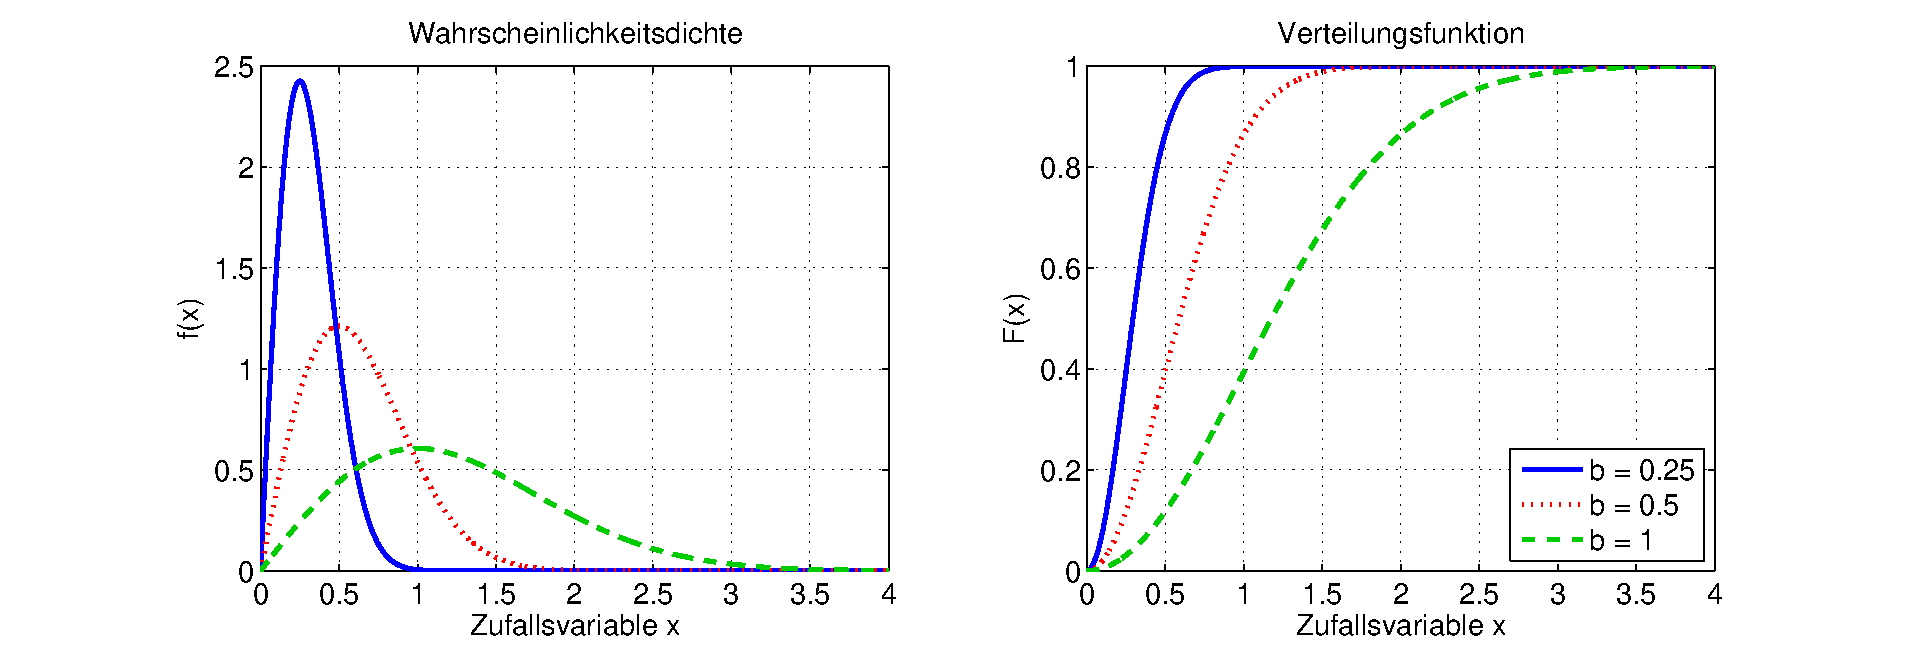
\includegraphics[width=1\textwidth]{Kapitel4/Bilder/image32}}
  \caption{Wahrscheinlichkeitsdichte f(x) und Verteilungsfunktion F(x) der Rayleigh-Verteilung}
  \label{fig:Stetig_Rayleigh}
\end{figure}

\noindent Die Rayleigh-Verteilung besitzt einen Mittelwert von

\begin{equation}\label{eq:fourtwohundredthree}
\mu =b\cdot \sqrt{\dfrac{\pi }{2}}
\end{equation}

\noindent Die Varianz der Rayleigh-Verteilung ergibt sich zu

\begin{equation}\label{eq:fourtwohundredfour}
\sigma ^{2} =\dfrac{4-\pi }{2} \cdot b^{2}
\end{equation}

\noindent Damit weist bei der Rayleigh-Verteilung das Verh\"{a}ltnis des Mittelwertes $\mu$ zur Standardabweichung $\sigma$ immer den festen Wert

\begin{equation}\label{eq:fourtwohundredfive}
\dfrac{\mu }{\sigma } =\sqrt{\dfrac{\pi }{4-\pi } } \approx 1.91
\end{equation}

\noindent auf.\bigskip

\noindent
\colorbox{lightgray}{%
\arrayrulecolor{white}%
\renewcommand\arraystretch{0.6}%
\begin{tabular}{ wl{16.5cm} }
{\fontfamily{phv}\selectfont
\noindent
Beispiel: Abstand einer Bohrung zu ihrer Sollposition}
\end{tabular}%
}\bigskip

\noindent Als Beispiel f\"{u}r die Anwendung der Rayleigh-Verteilung wird die Lage einer Bohrung betrachtet, die mittels einer Fertigungseinrichtung in eine Metallplatte gebohrt wird. Die Lage der Bohrungen unterliegt den Fertigungstoleranzen der Bohreinrichtung. Durch den Maschinenhersteller ist bekannt, dass die Abweichung der x- und y-Koordinaten vom Sollwert jeweils durch eine Normalverteilung mit einem Mittelwert $\mu_{x}$ = µ$_{y}$ = 0 $\mu$m und einer Standardabweichung von $\sigma_{x}$ = $\sigma_{y}$ = 0.25 $\mu$m beschrieben werden kann.\newline

\noindent Aus dem Satz von Pythagoras folgt, dass der Abstand $\Delta$z der Bohrung vom definierten Sollwert beschrieben werden kann durch

\begin{equation}\label{eq:fourtwohundredsix}
\Delta z=\sqrt{\left(\Delta x\right)^{2} +\left(\Delta y\right)^{2}}
\end{equation}

\noindent Die Verteilung der Gr\"{o}{\ss}e $\Delta$z ist eine Rayleigh-Verteilung mit dem Parameter b = 0.25. Diese ist in Bild \ref{fig:Stetig_Rayleigh_AbstandBohrung} zu sehen.

\begin{figure}[H]
  \centerline{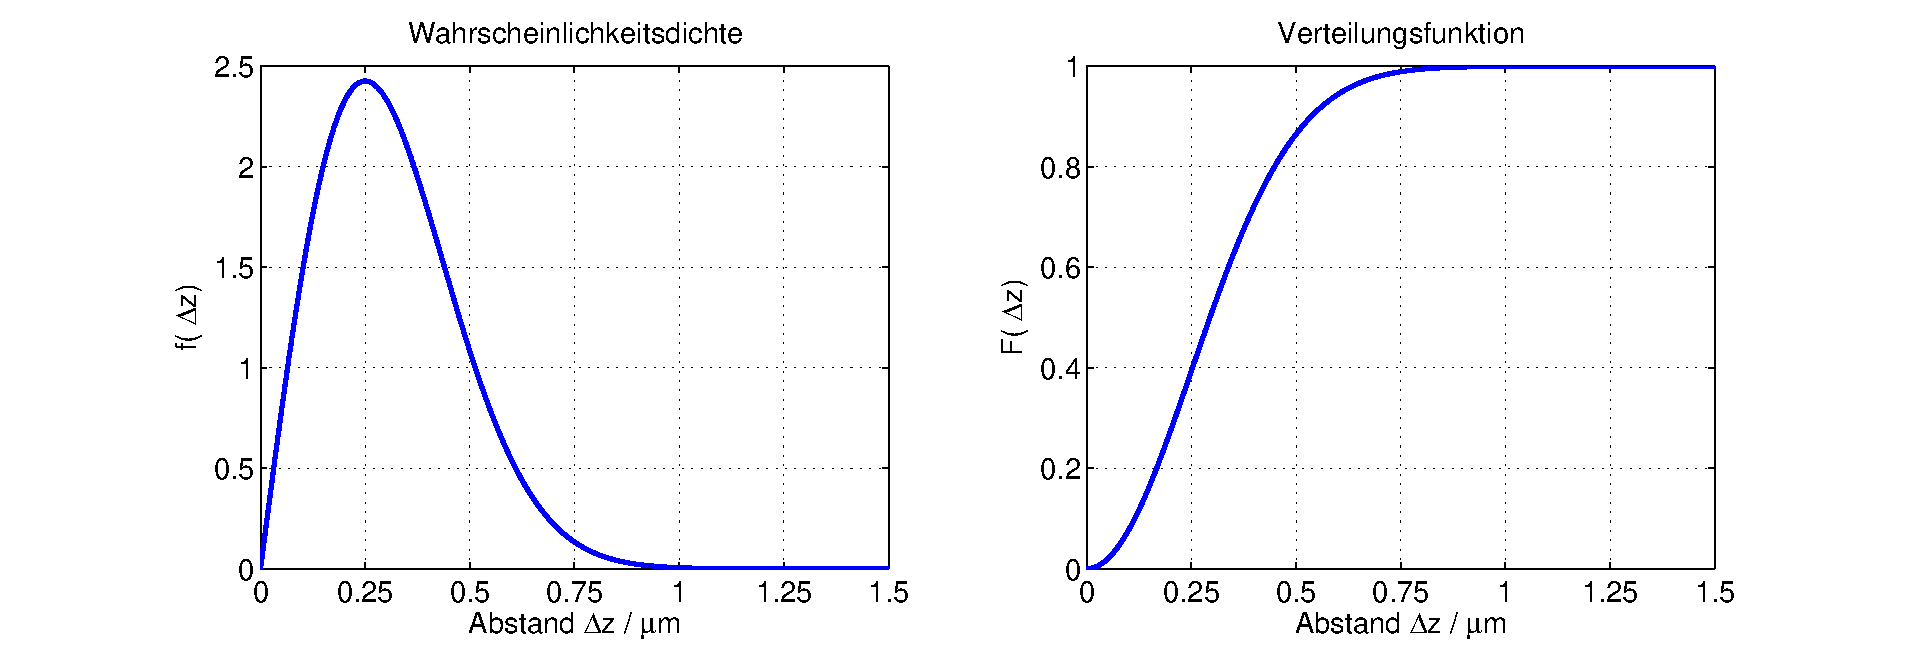
\includegraphics[width=1\textwidth]{Kapitel4/Bilder/image33}}
  \caption{Verteilung des Abstandes $\Delta$z einer Bohrung zu ihrer Sollposition}
  \label{fig:Stetig_Rayleigh_AbstandBohrung}
\end{figure}

\subsubsection{Normalverteilung}

\noindent Die Gau{\ss}- oder Normalverteilung wurde von Carl Friedrich Gau{\ss} im Zusammenhang mit dem Ausgleich von Messergebnissen gefunden. Sie ist die wichtigste stetige Verteilung, weil viele Messgr\"{o}{\ss}en oder Beobachtungen normalverteilt sind. Au{\ss}erdem lassen sich viele Verteilungen gut durch die Normalverteilung approximieren. Weiterhin kommen bei statistischen Pr\"{u}fverfahren oft Gr\"{o}{\ss}en vor, die entweder direkt normalverteilt sind oder sich bei Grenz\"{u}berg\"{a}ngen als normalverteilt beschreiben lassen.\bigskip

{\fontfamily{phv}\selectfont
\noindent\textbf{Allgemeine Definition der Normalverteilung}}

\noindent Die Wahrscheinlichkeitsdichte der Gau{\ss}- oder Normalverteilung ist f\"{u}r - $\infty$ $\mathrm{<}$ x  $\mathrm{<}$ $\infty$ definiert als

\begin{equation}\label{eq:fourtwohundredseven}
f(x)=\dfrac{1}{\sigma \cdot \sqrt{2\cdot \pi } } \cdot e^{-\dfrac{1}{2} \cdot \left(\dfrac{x-\mu }{\sigma } \right)^{2} }
\end{equation}

\noindent Eine Zufallsvariable x mit dieser Verteilung wird als normalverteilte Zufallsvariable bezeichnet. Sie besitzt die Parameter $\mu$ und $\sigma$. Bild \ref{fig:Stetig_Normalverteilung1} zeigt die Wahrscheinlichkeitsdichte der Normalverteilung mit einem Mittelwert von $\mu$ = 2 und verschiedenen Werten der Standard-abweichung $\sigma$.

\begin{figure}[H]
  \centerline{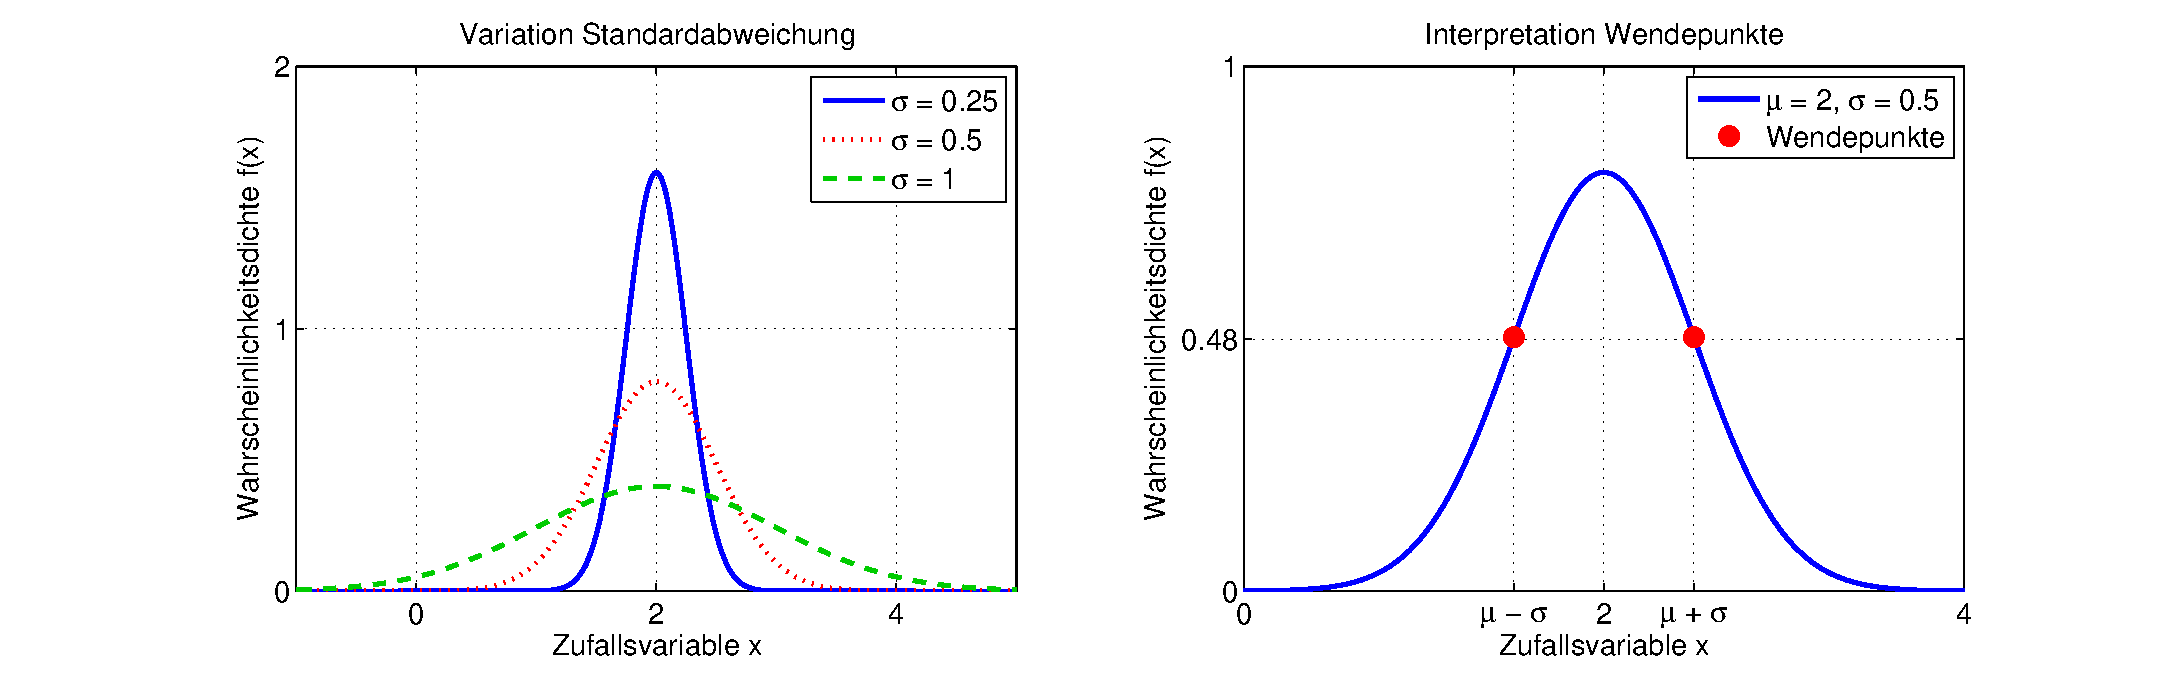
\includegraphics[width=1\textwidth]{Kapitel4/Bilder/image34}}
  \caption{Wahrscheinlichkeitsdichte f(x) f\"{u}r $\mu$ = 2 und $\sigma$ = 0.25, 0.5 und 1 und Lage der Wendepunkte}
  \label{fig:Stetig_Normalverteilung1}
\end{figure}

\noindent Aus der Symmetrie der Verteilung ergibt sich, dass das Maximum der Verteilung f\"{u}r den Mittelwert $\mu$ erreicht wird. Je kleiner $\sigma$ ist, desto schmaler ist die Verteilung und desto ausgepr\"{a}gter ist ihr Maximum. Je gr\"{o}{\ss}er $\sigma$ ist, desto breiter ist die Verteilung. Der Abstand der Wendepunkte der Wahrscheinlichkeitsdichte von dem Mittelwert $\mu$ entspricht der Standardabweichung $\sigma$.

\noindent Die Verteilungsfunktion F(x) hat die Form 

\begin{equation}\label{eq:fourtwohundredeight}
F(x)=\int\limits  _{-\infty }^{x}\dfrac{1}{\sigma \cdot \sqrt{2\cdot \pi } } \cdot e^{-\dfrac{1}{2} \cdot \left(\dfrac{\xi -\mu }{\sigma } \right)^{2} }  d\xi =\dfrac{1}{\sigma \cdot \sqrt{2\cdot \pi } } \cdot \int\limits  _{-\infty }^{x}e^{-\dfrac{1}{2} \cdot \left(\dfrac{\xi -\mu }{\sigma } \right)^{2} }  d\xi
\end{equation}

\noindent Die Verteilungsfunktion F(x) ist ein Integral, das sich nicht analytisch auswerten l\"{a}sst. Die Berechnung wird numerisch ausgef\"{u}hrt, zum Beispiel durch die numerische Integration \"{u}ber die Wahrscheinlichkeitsdichte f(x) oder mittels einer Approximation durch eine Taylor-Reihe.

\noindent Bild \ref{fig:Stetig_Normalverteilung2} zeigt die Verteilungsfunktion F(x) der Normalverteilung f\"{u}r $\mu$~= 2 und verschiedene Werte der Standardabweichung $\sigma$. 

\begin{figure}[H]
  \centerline{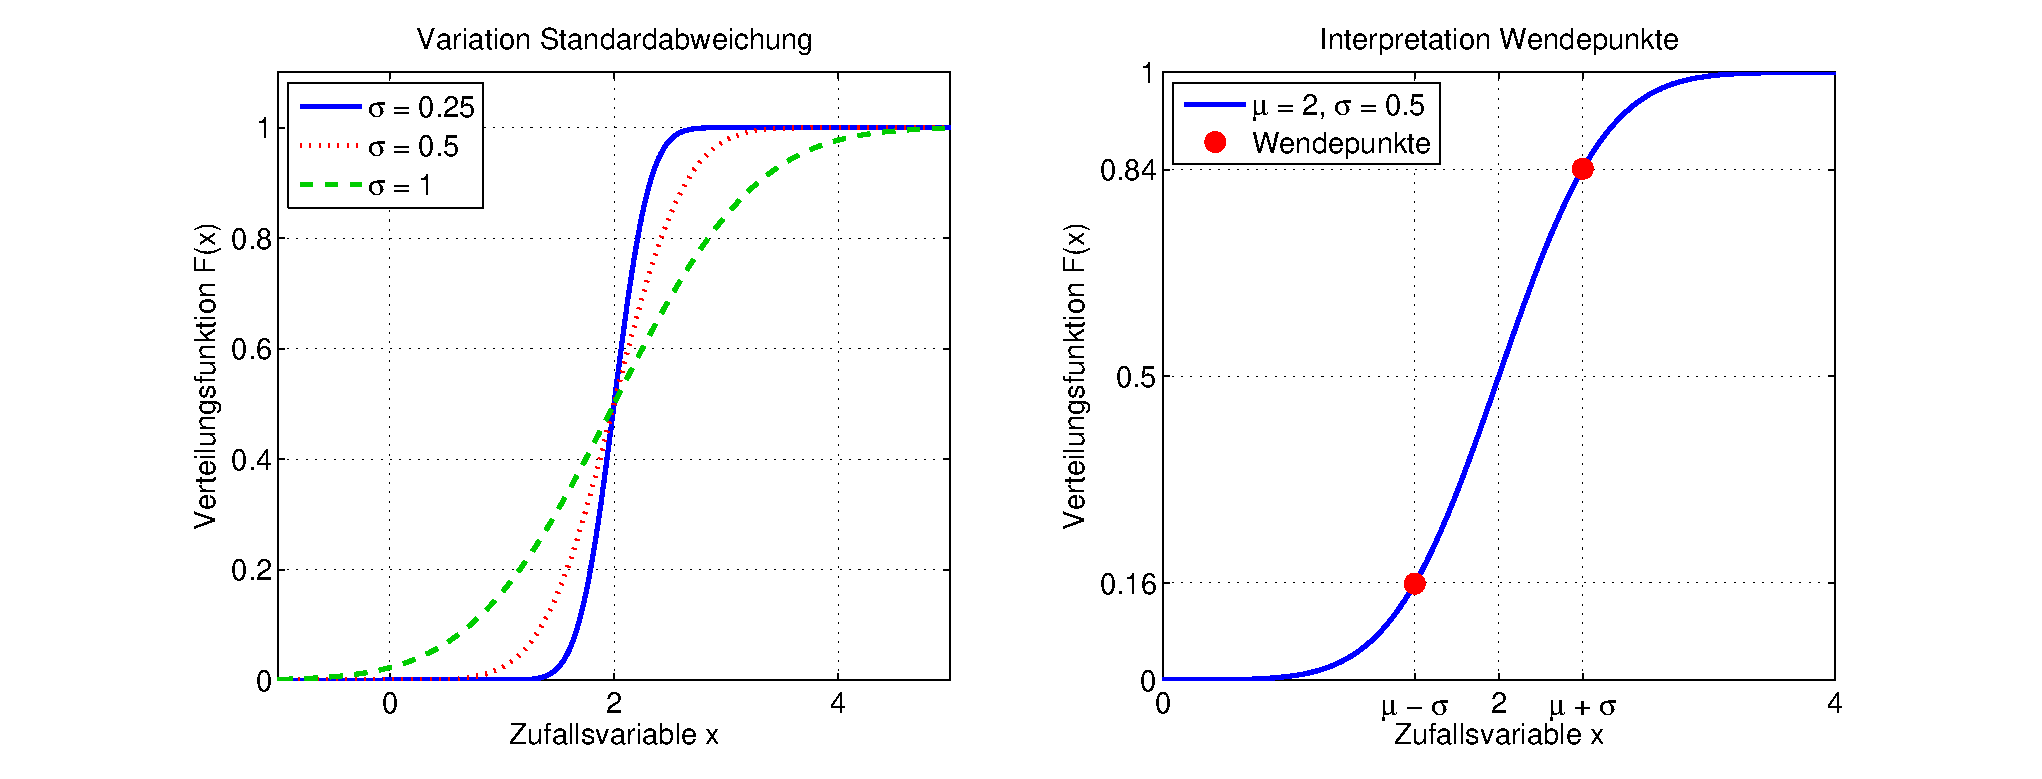
\includegraphics[width=1\textwidth]{Kapitel4/Bilder/image35}}
  \caption{Verteilungsfunktion F(x) f\"{u}r $\mu$ = 2 und $\sigma$ = 0.25, 0.5}
  \label{fig:Stetig_Normalverteilung2}
\end{figure}

\noindent F\"{u}r eine normalverteilte Variable x berechnet sich die Wahrscheinlichkeit P, innerhalb des Intervalls a $\mathrm{<}$ x $\leq$ b zu sein, aus 

\begin{equation}\label{eq:fourtwohundrednine}
P\left(a<x\le b\right)=F\left(b\right)-F\left(a\right)=\dfrac{1}{\sigma \cdot \sqrt{2\cdot \pi } } \cdot \int\limits  _{a}^{b}e^{-\dfrac{1}{2} \cdot \left(\dfrac{x-\mu }{\sigma } \right)^{2} }  dx
\end{equation}

\clearpage

{\fontfamily{phv}\selectfont
\noindent\textbf{Standardisierte Normalverteilung}}

\noindent Die Verteilungsfunktion der Normalverteilung kann nicht mehr analytisch berechnet werden. Durch eine Standardisierung der Zufallsvariablen werden alle Varianten der Normalverteilung auf eine standardisierte Form abgebildet, deren Wahrscheinlichkeitsdichte und Verteilungsfunktion in Form von Tabellen beschrieben ist. Bei der rechnerunterst\"{u}tzten Auswertung von Daten haben diese tabellierten Werte an Bedeutung verloren. Aus Gr\"{u}nden der \"{u}bersichtlicheren Darstellung und zur Vorbereitung der Rechnung mit Testverteilungen wird im Folgenden dennoch die standardisierte Normalverteilung eingef\"{u}hrt und f\"{u}r die weiteren Berechnungen eingesetzt. Bei der Standardisierung einer Verteilung wird analog zu Abschnitt 4.4.3 eine Standardisierung der Zufallsvariablen durchgef\"{u}hrt, sodass sie einen Mittelwert von $\mu$ = 0 und eine Standardabweichung von $\sigma$ = 1 erreicht. Nach den Ausf\"{u}hrungen in Abschnitt 4.4.3 f\"{u}hrt die Standardisierung der normalverteilten Zufallsvariable x zu einer standardnormalverteilten Zufallsvariable z durch den Ausdruck

\begin{equation}\label{eq:fourtwohundredten}
z=\dfrac{x-\mu _{x} }{\sigma _{x} }
\end{equation}

\noindent Dabei geht die Normalverteilung aus Gleichung \eqref{eq:fourtwohundredseven} \"{u}ber in die Standardnormalverteilung mit $\mu _{z}$ = 0 und $\sigma _{z}$ = 1. Die Dichtefunktion der standardisierten Normalverteilung vereinfacht sich damit gegen\"{u}ber Gleichung \eqref{eq:fourtwohundredseven} zu

\begin{equation}\label{eq:fourtwohundredeleven}
f(z)=\dfrac{1}{\sqrt{2\cdot \pi }} \cdot e^{-\dfrac{1}{2} \cdot z^{2}}
\end{equation}

\noindent Die zugeh\"{o}rige Verteilungsfunktion wird beschrieben durch

\begin{equation}\label{eq:fourtwohundredtwelve}
F(z)=\int\limits  _{-\infty }^{z}\dfrac{1}{\sqrt{2\cdot \pi}} \cdot e^{-\dfrac{1}{2} \cdot \zeta ^{2}}  d\zeta =\dfrac{1}{\sqrt{2\cdot \pi}} \cdot \int\limits  _{-\infty }^{z}e^{-\dfrac{1}{2} \cdot \zeta ^{2}}  d\zeta
\end{equation}

\noindent Die Wahrscheinlichkeitsdichte f(z) und die Verteilungsfunktion F(z) der Standardnormalverteilung ist in Bild \ref{fig:Stetig_Normalverteilung3} dargestellt.

\begin{figure}[H]
  \centerline{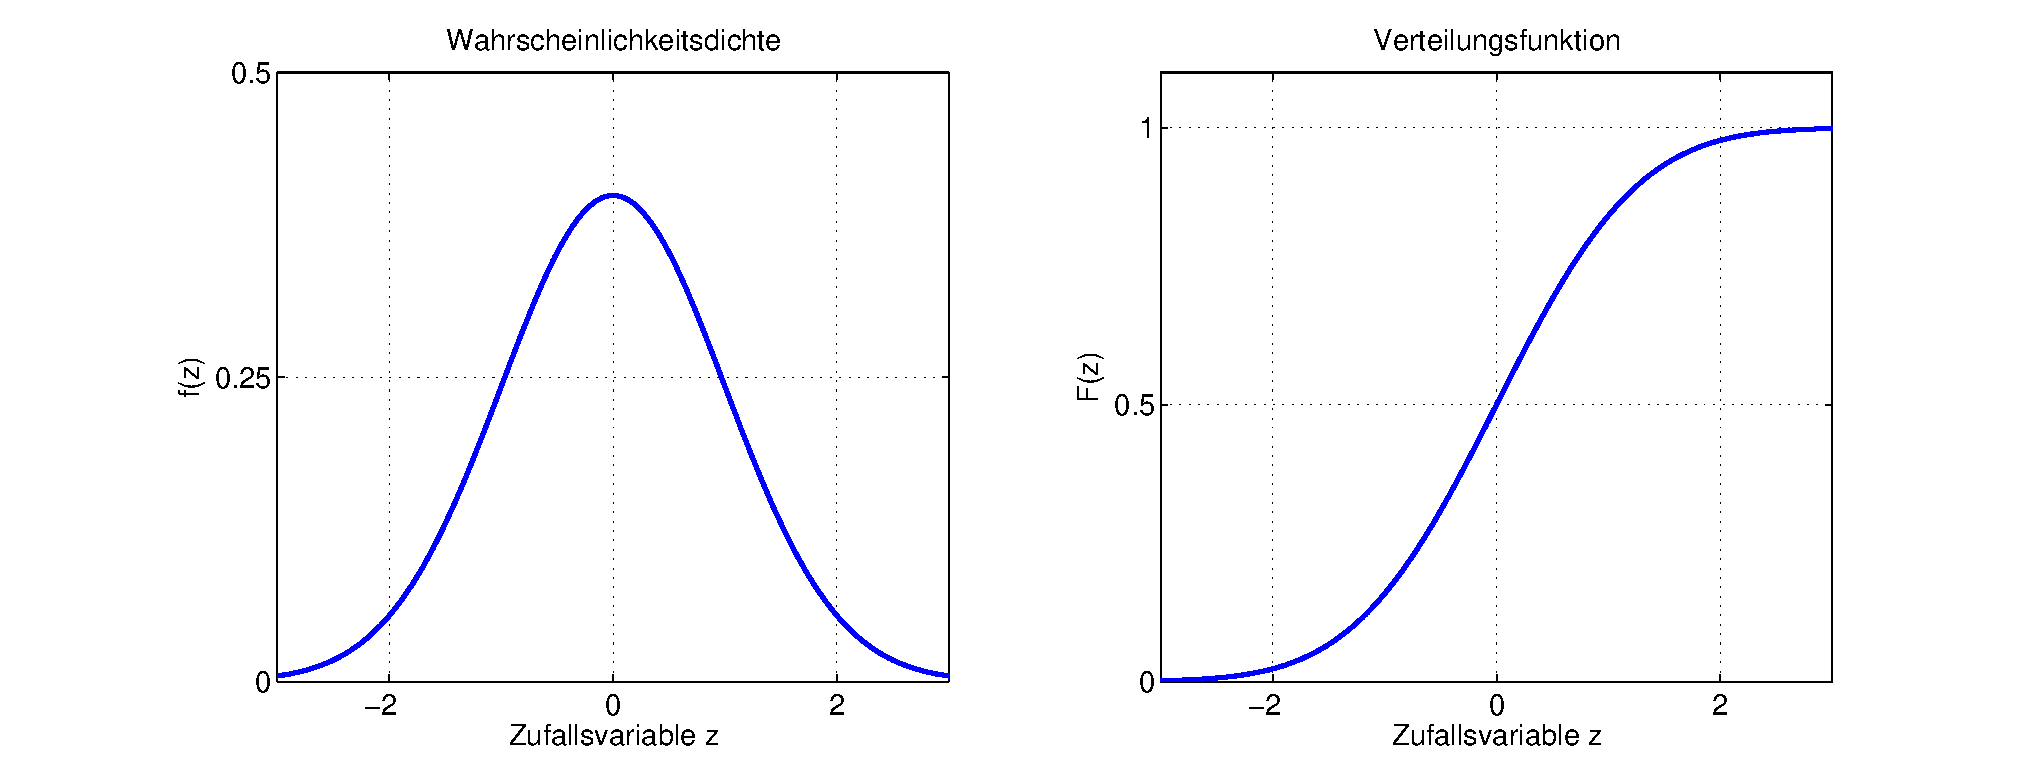
\includegraphics[width=1\textwidth]{Kapitel4/Bilder/image36}}
  \caption{Wahrscheinlichkeitsdichte f(z) und Verteilungsfunktion F(z) der Standardnormalverteilung}
  \label{fig:Stetig_Normalverteilung3}
\end{figure}

\noindent F\"{u}r eine standardnormalverteilte Variable z berechnet sich die Wahrscheinlichkeit P, innerhalb des Intervalls a $\mathrm{<}$ z $\leq$ b zu sein, aus 

\begin{equation}\label{eq:fourtwohundredthirteen}
P\left(a<x\le b\right)=F(b)-F(a)=\dfrac{1}{\sqrt{2\cdot \pi}} \cdot \int\limits _{a}^{b}e^{-\dfrac{1}{2} \cdot z^{2}}  dz
\end{equation}

\noindent Mit Gleichung \eqref{eq:fourtwohundredthirteen} k\"{o}nnen die Aufenthaltswahrscheinlichkeiten f\"{u}r eine standardnormalverteilte Zufallsvariable z in symmetrischen Intervallen errechnet werden.

\begin{table}[H]
\caption{Aufenthaltswahrscheinlichkeiten f\"{u}r eine standardnormalverteilte Zufallsvariable z}
\setlength{\fboxsep}{0pt}%
\colorbox{lightgray}{%
\arrayrulecolor{white}%
\begin{tabular}{| c | c |}
\hline
\parbox[c][0.28in][c]{3.3in}{\smallskip\centering\textbf{\fontfamily{phv}\selectfont{Intervall}}} & 
\parbox[c][0.28in][c]{3.3in}{\smallskip\centering\textbf{\fontfamily{phv}\selectfont{Aufenthaltswahrscheinlichkeit}}}\\ \hline

\parbox[c][0.3in][c]{3.3in}{\centering\fontfamily{phv}\selectfont{$- 1.\sigma \mathrm{<} z \leq 1.\sigma$}} &
\parbox[c][0.3in][c]{3.3in}{\centering\fontfamily{phv}\selectfont{$\approx 68.2689 \%$}} \\ \hline

\parbox[c][0.3in][c]{3.3in}{\centering\fontfamily{phv}\selectfont{$- 2.\sigma \mathrm{<} z \leq 2.\sigma$}} &
\parbox[c][0.3in][c]{3.3in}{\centering\fontfamily{phv}\selectfont{$\approx 95.4500 \%$}} \\ \hline

\parbox[c][0.3in][c]{3.3in}{\centering\fontfamily{phv}\selectfont{$- 3.\sigma \mathrm{<} z \leq 3.\sigma$}} &
\parbox[c][0.3in][c]{3.3in}{\centering\fontfamily{phv}\selectfont{$\approx 99.7300 \%$}} \\ \hline

\end{tabular}%
}\bigskip
\label{tab:fourfourteen}
\end{table}

\noindent Eine Abweichung vom Mittelwert um mehr als eine Standardabweichung ist etwa in einem von drei F\"{a}llen zu erwarten, eine Abweichung um mehr als drei Standardabweichungen nur in einem von 370 F\"{a}llen.\bigskip

\noindent
\colorbox{lightgray}{%
\arrayrulecolor{white}%
\renewcommand\arraystretch{0.6}%
\begin{tabular}{ wl{16.5cm} }
{\fontfamily{phv}\selectfont
\noindent
Beispiel: Zusammenhang zwischen Toleranzziel und Ausschuss bei der Fertigung}
\end{tabular}%
}\bigskip

\noindent Als Beispiel f\"{u}r die Normalverteilung soll der Zusammenhang zwischen Toleranzziel und Ausschuss bei der Fertigung von Widerst\"{a}nden betrachtet werden. Von einem Fertigungslos von 10000 Widerst\"{a}nden sei bekannt, dass die Widerstandsverteilung als Normalverteilung mit dem Mittelwert $\mu$ = 998=? und einer Standardabweichung von $\sigma$ = 5 ? dargestellt werden kann. Es werden unterschiedliche Kunden beliefert. Kunde A fordert ein Toleranzziel von

\begin{equation}\label{eq:fourtwohundredfourteen}
R_{A} =1000 \Omega \pm 10 \Omega
\end{equation}

\noindent Kunde B fordert ein Toleranzziel von 

\begin{equation}\label{eq:fourtwohundredfifteen}
R_{B} =1000 \Omega \pm 20 \Omega
\end{equation}

\noindent F\"{u}r beide Kunden soll der Anteil von Ausschussteilen berechnet werden. Da die Widerstandswerte eine Normalverteilung mit $\mu$ = 998 ? und $\sigma$ = 5 ? besitzen, ergibt sich der Anteil von Ausschussteilen aus

\begin{equation}\label{eq:fourtwohundredsixteen}
A_{A} =F\left(z=\dfrac{990-998}{5} \right)+1-F\left(z=\dfrac{1010-998}{5} \right)=6.3 \%
\end{equation}

\noindent Mit den Toleranzgrenzen von Kunde B ergibt sich

\begin{equation}\label{eq:fourtwohundredseventeen}
A_{B} =F\left(z=\dfrac{980-998}{5} \right)+1-F\left(z=\dfrac{1020-998}{5} \right)=0.02 \%
\end{equation}

\noindent F\"{u}r Kunde B ist der Ausschussanteil wegen des doppelt so gro{\ss}en Toleranzbereiches um mehr als zwei Gr\"{o}{\ss}enordnungen geringer. Durch eine Zentrierung des Mittelwertes von $\mu$ = 998 ? auf $\mu$ = 1000 ? lie{\ss}e sich der Ausschussanteil zudem auf 4.5 \% beziehungsweise 63 ppm reduzieren.

\noindent Die Werte nach Gleichung \eqref{eq:fourtwohundredsixteen} und \eqref{eq:fourtwohundredseventeen} berechnen sich mit der folgenden MATLAB-Sequenz:

\clearpage

\lstinputlisting[caption = {}]{Kapitel4/mat15.m}

\noindent Entsprechend ergibt sich in Python:

\lstinputlisting[caption = {}]{Kapitel4/mat16.m}

\subsubsection{Logarithmische Normalverteilung}

\noindent Verteilungen von nicht negativen Zufallsvariablen sind oft nicht symmetrisch. Verteilungen von Lebensdauern, Wartezeiten oder Einkommen sind rechtsschief und k\"{o}nnen deshalb nicht direkt mit der Normalverteilung beschrieben werden. In einigen F\"{a}llen kann die Verteilung durch die Exponential-, Rayleigh- oder Weibull-Verteilung erfolgen. Eine weitere M\"{o}glichkeit zur Beschreibung ist die logarithmische Normalverteilung. Die logarithmische Normalverteilung ist definiert durch die Zufallsvariable y, die sich aus der Exponentialfunktion der normalverteilten Zufallsvariable x ergibt.

\begin{equation}\label{eq:fourtwohundredeighteen}
y=g(x)=e^{x}
\end{equation}

\noindent Die Wahrscheinlichkeitsdichte f${}_{Y}$(y) ergibt sich durch die Variablentransformation der in Gleichung \eqref{eq:fourtwohundredeighteen} dargestellten Form durch

\begin{equation}\label{eq:fourtwohundrednineteen}
f_{Y} (y)=f_{X} \left(g^{-1} (y)\right)\cdot \left|\dfrac{dg^{-1} (y)}{dy} \right|
\end{equation}

\noindent Mit der Umkehrfunktion 

\begin{equation}\label{eq:fourtwohundredtwenty}
x=\ln (y)
\end{equation}

\noindent ergibt sich die Wahrscheinlichkeitsdichte f${}_{Y}$(y) 

\begin{equation}\label{eq:fourtwohundredtwentyone}
f_{Y} (y)=\dfrac{1}{\sigma _{x} \cdot \sqrt{2\cdot \pi } } \cdot \dfrac{1}{y} \cdot e^{-\dfrac{1}{2} \cdot \left(\dfrac{\ln (y)-\mu _{x} }{\sigma _{x} } \right)^{2} }
\end{equation}

\noindent und die Verteilungsfunktion F$_{Y}$(y) lautet

\begin{equation}\label{eq:fourtwohundredtwentytwo}
F_{Y} (y)=\dfrac{1}{\sigma _{x} \cdot \sqrt{2\cdot \pi } } \cdot \int _{-\infty }^{y}\dfrac{1}{\psi } \cdot e^{-\dfrac{1}{2} \cdot \left(\dfrac{\ln (\psi )-\mu _{x} }{\sigma _{x} } \right)^{2} }  d\psi
\end{equation}

\noindent Bild \ref{fig:Stetig_Lognormal1} stellt f\"{u}r Exponential-Verteilungen mit Mittelwert $\mu_{x}$ = 0 und unterschiedlicher Standardabweichung $\sigma_{x}$ die Wahrscheinlichkeitsdichte f$_{Y}$(y) und Verteilungsfunktion F$_{Y}$(y) dar.

\begin{figure}[H]
  \centerline{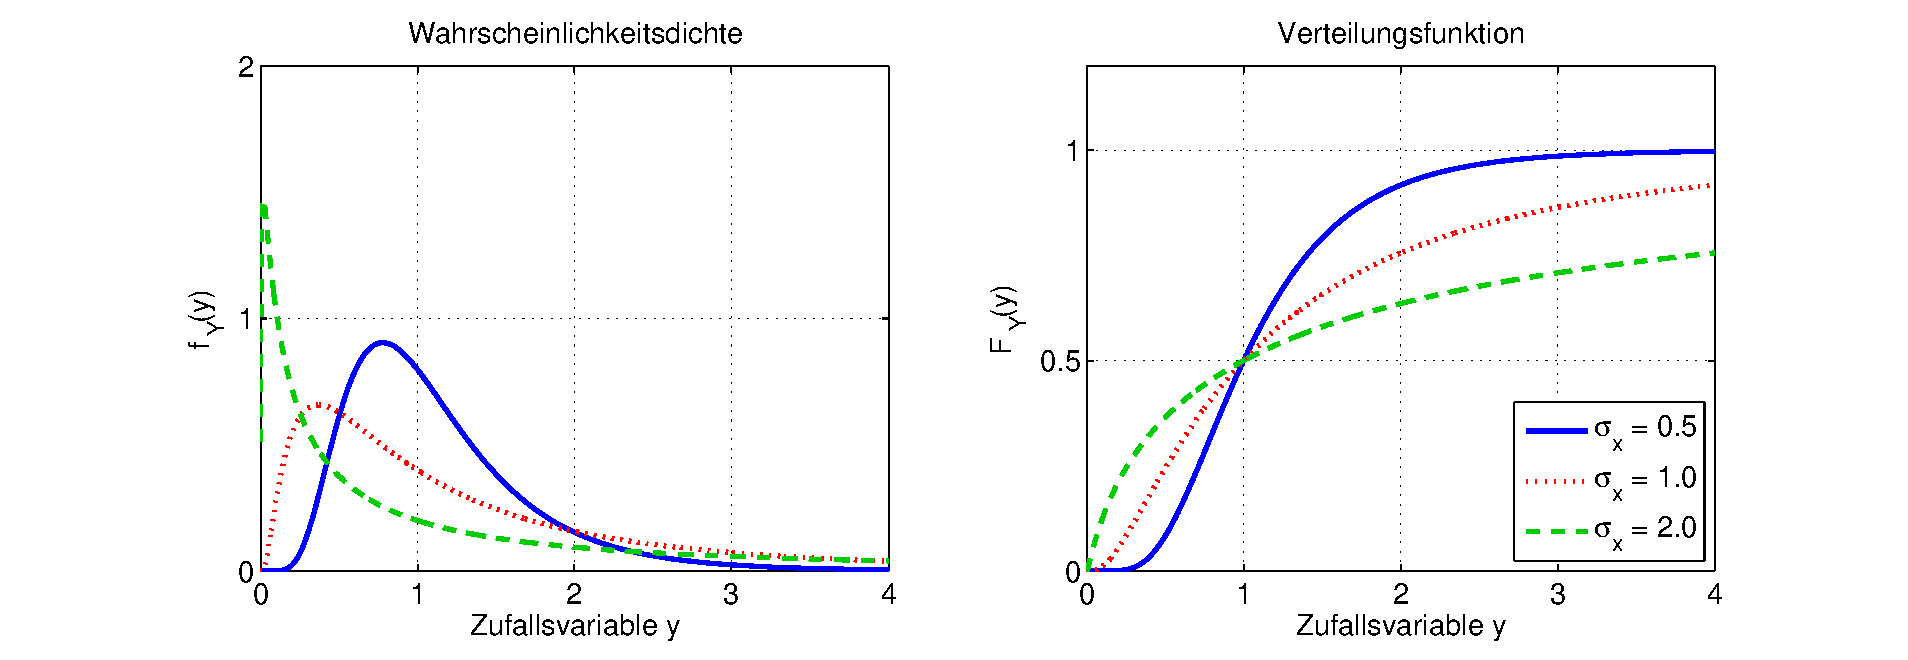
\includegraphics[width=1\textwidth]{Kapitel4/Bilder/image37}}
  \caption{Wahrscheinlichkeitsdichte f${}_{Y}$(y) und Verteilungsfunktion F${}_{Y}$(y) der logarithmischen Normalverteilung f\"{u}r $\mu_{X}$ = 0 und $\sigma_{X}$ = 0.5, 1 und 2}
  \label{fig:Stetig_Lognormal1}
\end{figure}

\noindent Mittelwert $\mu_{Y}$ und Varianz $\sigma_{Y}^{2}$ k\"{o}nnen als Funktion des Mittelwertes $\mu_{X}$ und Varianz $\sigma_{X}^{2}$ der nicht logarithmierten Gr\"{o}{\ss}en dargestellt werden als 

\begin{equation}\label{eq:fourtwohundredtwentythree}
\mu _{Y} =e^{\mu _{X} +\dfrac{\sigma _{X}^{2} }{2}}
\end{equation}

\noindent und

\begin{equation}\label{eq:fourtwohundredtwentyfour}
\sigma _{Y}^{2} =e^{2\cdot \mu _{X} +\sigma _{X}^{2} } \cdot \left(e^{\sigma _{X}^{2} } -1\right)
\end{equation}

\noindent Die Verteilungsfunktion der logarithmischen Normalverteilung kann im doppelt logarithmisch geteilten Wahrscheinlichkeitspapier durch zwei Geraden angen\"{a}hert werden. Die Approximation der Verteilungsfunktion durch Geradengleichungen wird mit steigendem Wert f\"{u}r $\sigma_{X}$ besser, wie in Bild \ref{fig:Stetig_Lognormal2} zu sehen ist.

\begin{figure}[H]
  \centerline{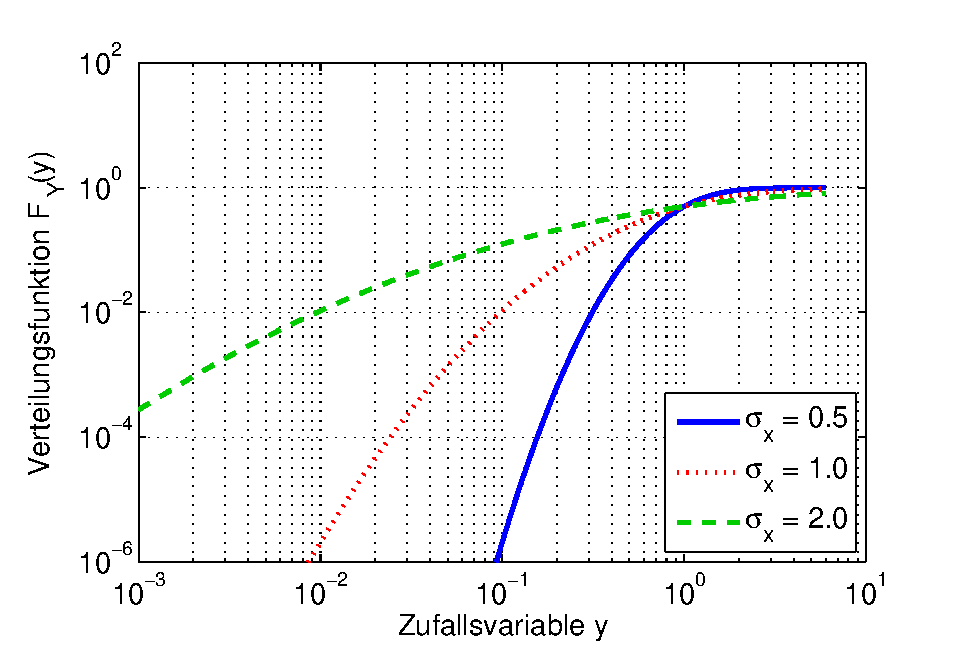
\includegraphics[width=0.5\textwidth]{Kapitel4/Bilder/image38}}
  \caption{Verteilungsfunktion F${}_{Y}$(y) der logarithmischen Normalverteilung f\"{u}r $\mu_{X}$ = 0 und $\sigma_{X}$ = 0.5, 1 und 2 im doppelt logarithmischen Ma{\ss}stab}
  \label{fig:Stetig_Lognormal2}
\end{figure}

\noindent
\colorbox{lightgray}{%
\arrayrulecolor{white}%
\renewcommand\arraystretch{0.6}%
\begin{tabular}{ wl{16.5cm} }
{\fontfamily{phv}\selectfont
\noindent
Beispiel: Rauigkeit einer Oberfl\"{a}che}
\end{tabular}%
}\bigskip

\noindent Als Beispiel f\"{u}r die Anwendung der Logarithmischen Normalverteilung wird die Verteilung der Rauigkeit einer Oberfl\"{a}che dargestellt. Die Untersuchung einer Oberfl\"{a}che hat ergeben, dass die Verteilung der Rauigkeit durch eine logarithmische Normalverteilung mit einem Mittelwert von $\mu_{R}$ = 1.78 nm und einer Standardabweichung von $\sigma_{R}$= 0.65 nm beschrieben werden kann. Bild \ref{fig:Lognormal_Oberflaechenrauheit} stellt die festgestellte Wahrscheinlichkeitsdichte f(R) und die Verteilungsfunktion F(R) der Rauheit R dar.

\begin{figure}[H]
  \centerline{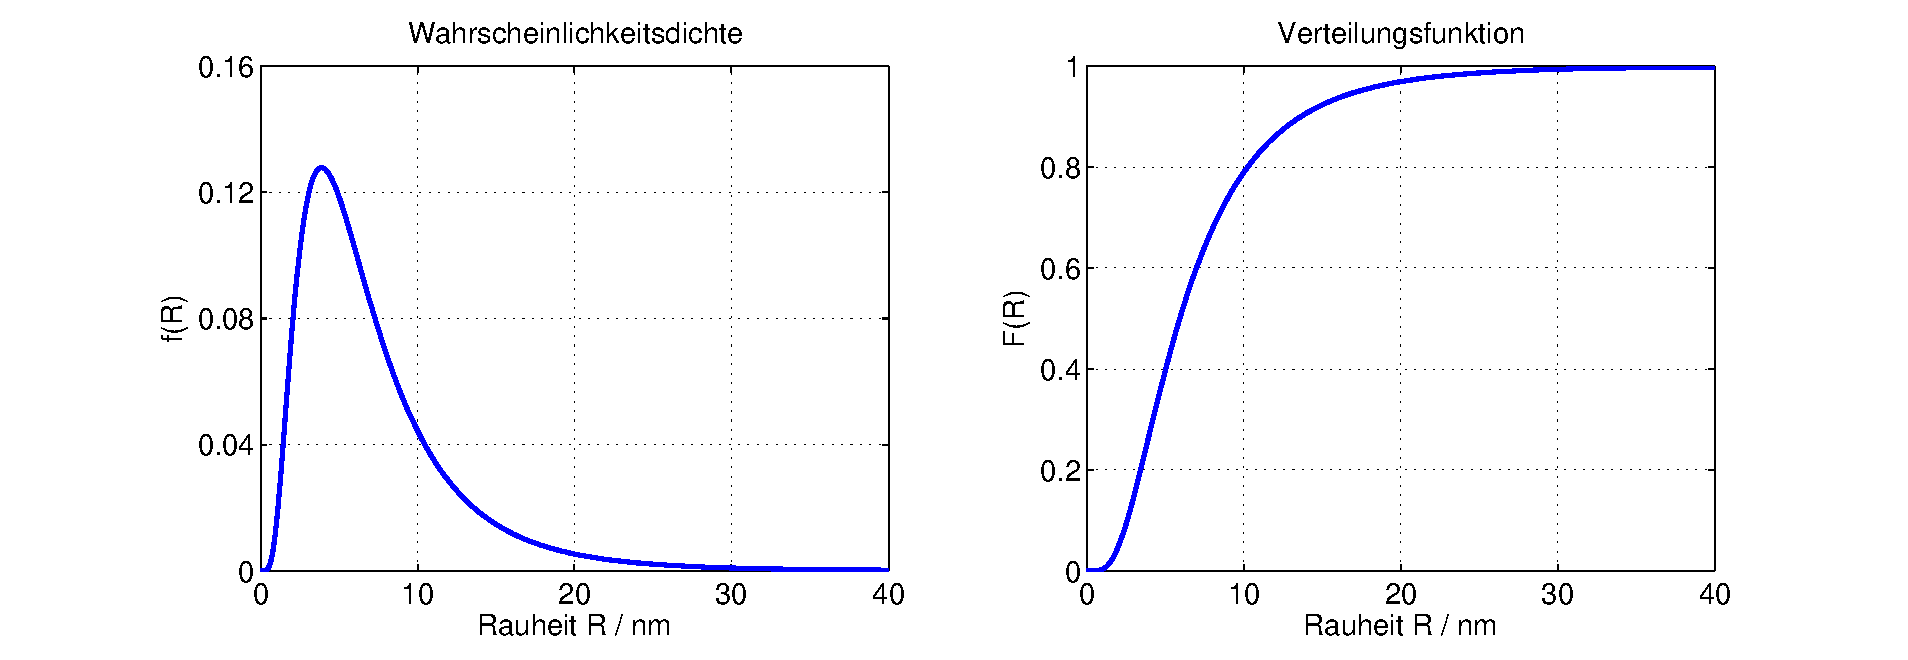
\includegraphics[width=1\textwidth]{Kapitel4/Bilder/image39}}
  \caption{Darstellung der Verteilung der Rauheit R einer Oberfl\"{a}che}
  \label{fig:Lognormal_Oberflaechenrauheit}
\end{figure}

\noindent Der Wert der Rauigkeit kann nicht kleiner als 0 werden. Dies f\"{u}hrt zu einer rechtsschiefen Verteilung.

\subsubsection{Betragsverteilung 1. Art}

\noindent Wird die Normalverteilung an einem beliebigen Punkt unterhalb des Mittelwertes $\mu$ gefaltet, f\"{u}hrt dies zur Betragsverteilung 1. Art. Durch die Faltung werden die Werte links des Faltungspunktes denen rechts vom Faltungspunkt additiv \"{u}berlagert. Dabei entsteht die Wahrscheinlichkeitsdichte f(x) der Betragsverteilung 1. Art zu

\begin{equation}\label{eq:fourtwohundredtwentyfive}
f(x)=\left\{\begin{array}{c} {\dfrac{1}{\sigma \cdot \sqrt{2\cdot \pi}} \cdot \left(e^{-\dfrac{1}{2} \cdot \left(\dfrac{x-\mu}{\sigma} \right)^{2}} +e^{-\dfrac{1}{2} \cdot \left(\dfrac{x+\mu }{\sigma} \right)^{2}} \right)\text{ für } x\ge 0} \\ 
{0 \qquad \qquad \text{ für } x<0} \end{array}\right.
\end{equation}

\noindent Die Verteilungsfunktion F(x) folgt durch Integration zu

\begin{equation}\label{eq:fourtwohundredtwentysix}
F\left(x\right)=\left\{\begin{array}{c} {\dfrac{1}{\sigma \cdot \sqrt{2\cdot \pi } } \cdot \int\limits _{0}^{x}\left(e^{-\dfrac{1}{2} \cdot \left(\dfrac{\xi -\mu }{\sigma } \right)^{2} } +e^{-\dfrac{1}{2} \cdot \left(\dfrac{\xi +\mu }{\sigma } \right)^{2} } \right) d\xi \text{ für } x\ge 0} \\ 
{0 \qquad \qquad \text{ für } x<0} \end{array}\right.
\end{equation}

\noindent Die Wahrscheinlichkeitsdichte f(x) der Betragsverteilung 1. Art ist in Bild 4.40Bild 4.40 zu sehen. Die linke Grafik zeigt die Faltung an der Stelle x = 0 einer Normalverteilung mit einem Mittelwert $\mu$ = 0.75 und einer Standardabweichung $\sigma$ = 0.5. Ein Sonderfall stellt die Faltung an der Stelle x = $\mu$ dar. Dabei vereinfacht sich die Definitionsgleichung Gleichung \eqref{eq:fourtwohundredtwentyfive} der Betragsverteilung 1. Art zu

\begin{equation}\label{eq:fourtwohundredtwentyseven}
f\left(x\right)=\left\{\begin{array}{c} {\dfrac{2}{\sigma \cdot \sqrt{2\cdot \pi } } \cdot e^{-\dfrac{1}{2} \cdot \left(\dfrac{x}{\sigma } \right)^{2} } \text{ für } x\ge 0} \\ 
{0 \qquad \qquad \text{ für } x<0} \end{array}\right.
\end{equation}

\noindent Dies entspricht der rechten Grafik in Bild \ref{fig:Stetig_Betragsverteilung1Art}. Hierbei wurde eine Normalverteilung mit einem Mittelwert $\mu$ = 1 und einer Standardabweichung $\sigma$ = 0.5 an der Stelle des Mittelwertes $\mu$ gefaltet.

\begin{figure}[H]
  \centerline{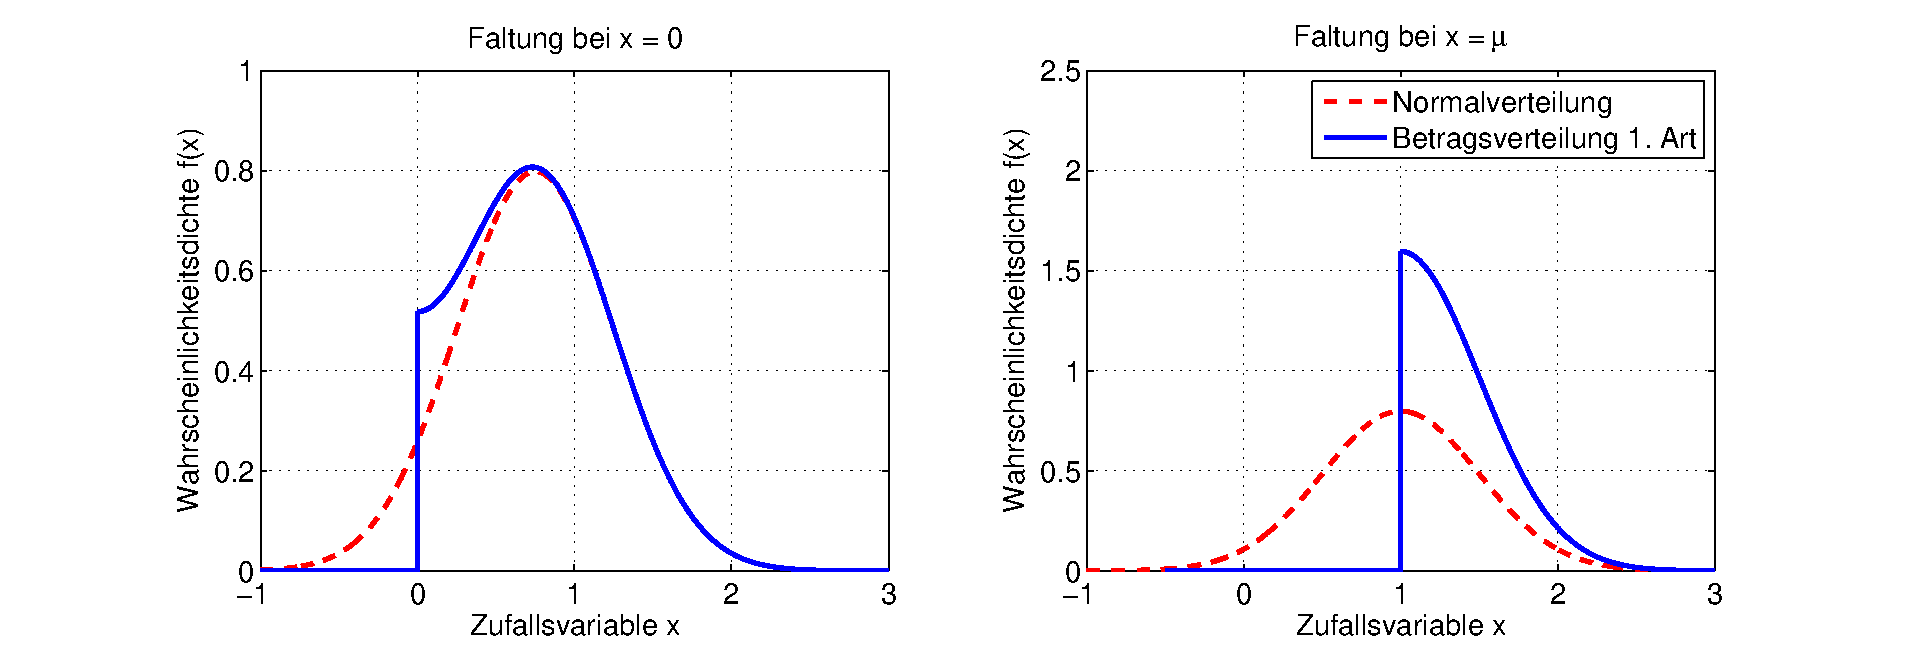
\includegraphics[width=1\textwidth]{Kapitel4/Bilder/image40}}
  \caption{Wahrscheinlichkeitsdichte f(x) der gefalteten Normalverteilung}
  \label{fig:Stetig_Betragsverteilung1Art}
\end{figure}

\noindent Die Betragsverteilung 1. Art wird zur Bewertung der Prozesssicherheit im Rahmen der statistischen Prozesskontrolle eingesetzt.\bigskip

\noindent
\colorbox{lightgray}{%
\arrayrulecolor{white}%
\renewcommand\arraystretch{0.6}%
\begin{tabular}{ wl{16.5cm} }
{\fontfamily{phv}\selectfont
\noindent
Beispiel: Verteilung der Abweichung vom Sollwert bei der Widerstandsfertigung}
\end{tabular}%
}\bigskip

\noindent Die Anwendung der Betragsverteilung 1. Art wird an einem Beispiel der Widerstandsfertigung verdeutlicht. Hierzu wird eine normalverteilte Widerstandsproduktion betrachtet, bei der die Widerstandswerte mit einer Standardabweichung von $\sigma$ = 0.75 $\Omega$ um den Sollwert streuen. Der Betrag dieser Abweichungen vom Sollwert {\textbar}$\Delta$R{\textbar} der Fertigung kann mithilfe der Betragsverteilung 1. Art beschrieben werden.\newline

\noindent In der linken Grafik in Bild \ref{fig:Stetig_Betragsverteilung1Art_Widerstandsfertigung1} ist die Wahrscheinlichkeitsdichte f($\Delta$R) der Wahrscheinlichkeitsdichte f({\textbar}$\Delta$R{\textbar}) gegen\"{u}bergestellt. Die rechte Grafik zeigt die entsprechenden Verteilungsfunktionen F($\Delta$R) und F({\textbar}$\Delta$R{\textbar}).

\begin{figure}[H]
  \centerline{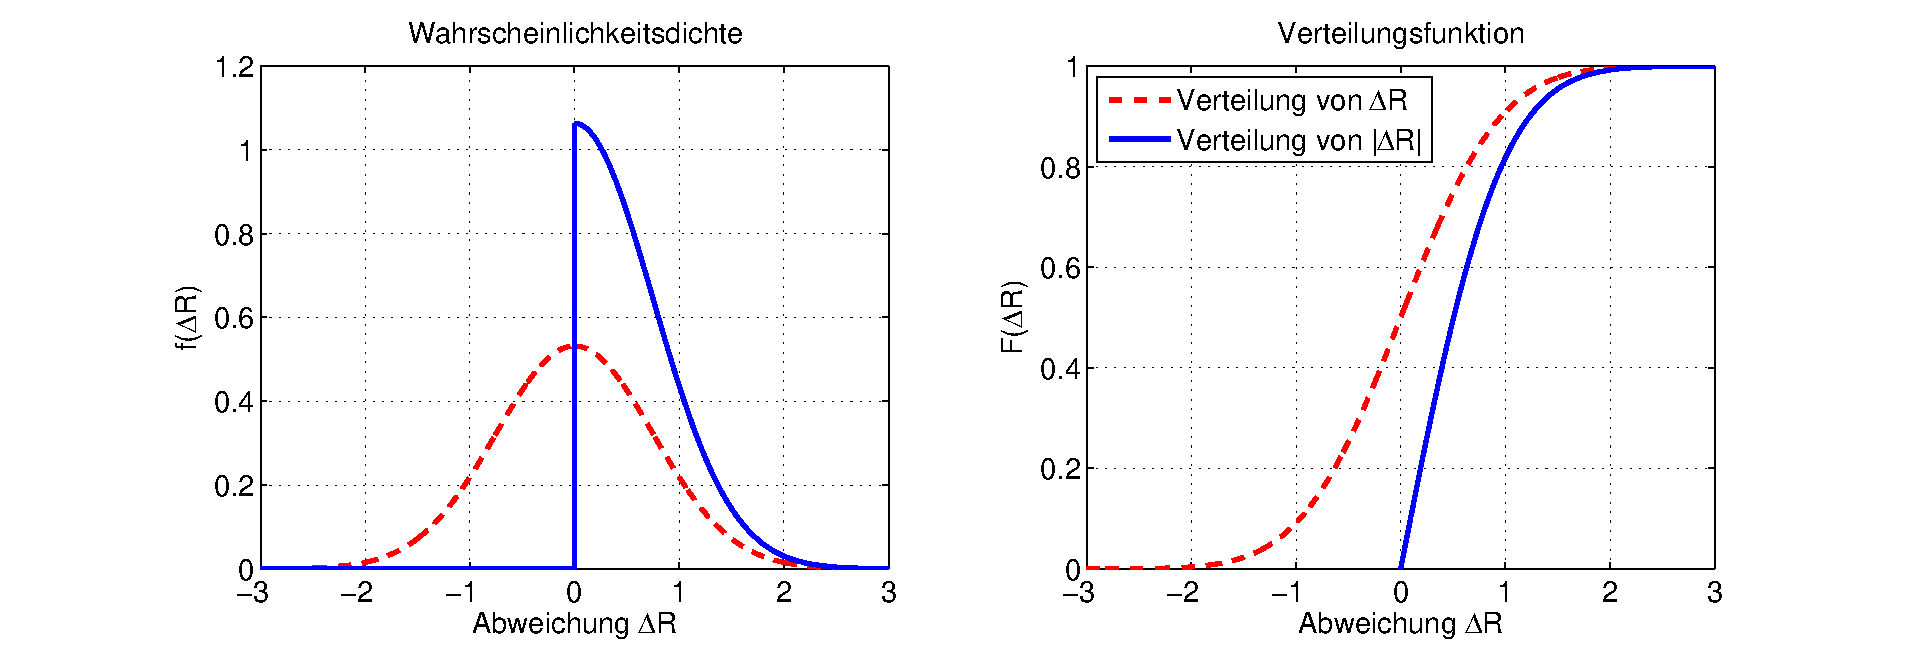
\includegraphics[width=1\textwidth]{Kapitel4/Bilder/image41}}
  \caption{Wahrscheinlichkeitsdichte f($\Delta$R) beziehungsweise f({\textbar}$\Delta$R{\textbar}) und Verteilungsfunktion F($\Delta$R) beziehungsweise F({\textbar}$\Delta$R{\textbar}) der Widerstandsabweichung vom Sollwert}
  \label{fig:Stetig_Betragsverteilung1Art_Widerstandsfertigung1}
\end{figure}

\subsubsection{Zusammenfassung der stetigen Verteilungen}

\noindent In diesem Abschnitt werden spezielle stetige Verteilungen vorgestellt und an Beispielen diskutiert. Dabei wird auch gezeigt, dass unter gewissen Randbedingungen die Verteilungen ineinander \"{u}bergehen. Bild \ref{fig:Stetig_Betragsverteilung1Art_Widerstandsfertigung2} stellt diese Zusammenh\"{a}nge grafisch dar und gibt damit zus\"{a}tzlich einen \"{U}berblick \"{u}ber die wichtigsten stetigen Verteilungen.

\begin{figure}[H]
  \centerline{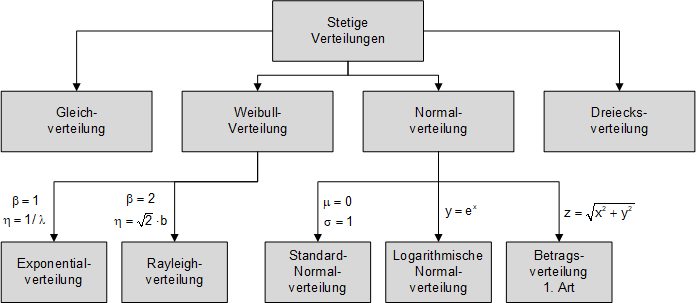
\includegraphics[width=1\textwidth]{Kapitel4/Bilder/image42}}
  \caption{Zusammenhang der stetigen Verteilungen}
  \label{fig:Stetig_Betragsverteilung1Art_Widerstandsfertigung2}
\end{figure}

\noindent Die diskutierten stetigen Wahrscheinlichkeitsverteilungen sind in Tabelle \ref{tab:fourfifteen} zusammenfassend dargestellt.

\noindent Wie bereits bei den diskreten Verteilungen im vorigen Abschnitt werden auch f\"{u}r kontinuierliche Verteilungsfunktionen die entsprechenden MATLAB-Befehle der Statistic Toolbox tabellarisch vorgestellt. Dabei gelten die bereits eingef\"{u}hrten Endungen. Tabelle \ref{tab:foursixteen} zeigt eine \"{U}bersicht der MATLAB-Funktionen \"{u}ber die Auswahl der stetigen Verteilungen aus diesem Abschnitt.

\clearpage

\begin{table}[H]
\setlength{\arrayrulewidth}{.1em}
\caption{\"{U}bersicht \"{u}ber diskrete Wahrscheinlichkeitsverteilungen}
\setlength{\fboxsep}{0pt}%
\colorbox{lightgray}{%
\arrayrulecolor{white}%
\begin{tabular}{| c | c | c |}
\hline
\parbox[c][0.3in][c]{1.9in}{\smallskip\centering\textbf{\fontfamily{phv}\selectfont{Name und Anwendung}}} &
\parbox[c][0.3in][c]{2.6in}{\smallskip\centering\textbf{\fontfamily{phv}\selectfont{Wahrscheinlichkeitsverteilung}}} &
\parbox[c][0.3in][c]{1.9in}{\smallskip\centering\textbf{\fontfamily{phv}\selectfont{Kenngr\"{o}{\ss}en $\mu$ und $\sigma ^{2}$}}}\\ \hline

\parbox[c][1.2in][c]{1.9in}{\centering\fontfamily{phv}\selectfont{Gleichverteilung: \newline
\\
Beschreibung von Wartezeiten und Diskretisierungsvorgängen
}} & 
\parbox[c][1.2in][c]{2.6in}{\centering\fontfamily{phv}\selectfont{$f(x)=\dfrac{1}{b-a} $}} &
\parbox[c][1.2in][c]{1.9in}{\centering\fontfamily{phv}\selectfont{$\mu =\dfrac{a+b}{2} \cdot \sum _{n=1}^{N}x_{n} $\bigskip

$\sigma ^{2} =\dfrac{(b-a)^{2}}{12} $}}\\
\hline

\parbox[c][1.2in][c]{1.9in}{\centering\fontfamily{phv}\selectfont{Symmetrische 
Dreiecksverteilung:\newline
\\
Toleranzverteilung bei Fertigungsprozessen}} & 
\parbox[c][1.2in][c]{2.6in}{\centering\fontfamily{phv}\selectfont{$f(x)=\left\{\begin{array}{ll} 
\dfrac{4}{(b-a)^{2}}\cdot (x-a)  \text{ für } a < x < \mu \\
\\
\dfrac{-4}{(b-a)^{2}}\cdot (b-x)  \text{ für }  \mu < x < a
\end{array}\right. $}} &
\parbox[c][1.2in][c]{1.9in}{\centering\fontfamily{phv}\selectfont{$\mu =\dfrac{a+b}{2} \cdot \sum _{n=1}^{N}x_{n} $\bigskip

$\sigma ^{2} =\dfrac{(b-a)^{2}}{24} $}}\\
\hline

\parbox[c][1.6in][c]{1.9in}{\centering\fontfamily{phv}\selectfont{Weibull-Verteilung:\newline
\\
Lebensdauer von 
Produkten, Zeiträumen bis zum Schadensfall, Ausfall-wahrscheinlichkeit ändert sich über der Beobachtungs-zeit}} & 
\parbox[c][1.6in][c]{2.6in}{\centering\fontfamily{phv}\selectfont{$f(x)=\dfrac{\beta}{\mu}\cdot \left(\dfrac{x}{\mu} \right)^{\beta -1} \cdot e^{-\left(\dfrac{x}{\mu} \right)^{\beta}} $}} &
\parbox[c][1.6in][c]{1.9in}{\centering\fontfamily{phv}\selectfont{siehe Abschnitt\\
4.6.3}}\\
\hline

\parbox[c][1.6in][c]{1.9in}{\centering\fontfamily{phv}\selectfont{Exponential-Verteilung:
\newline
\\
Lebensdauer von Produkten, Zeiträumen bis zum Schadensfall, Ausfallwahrscheinlichkeit ändert sich nicht über der Beobachtungszeit}} & 
\parbox[c][1.6in][c]{2.6in}{\centering\fontfamily{phv}\selectfont{$f(x)=\lambda \cdot e^{-\lambda\cdot x}$}} &
\parbox[c][1.6in][c]{1.9in}{\centering\fontfamily{phv}\selectfont{$\mu =\dfrac{1}{\lambda} $ \bigskip

$\sigma ^{2} =\dfrac{1}{\lambda ^{2}} $}}\\
\hline

\parbox[c][1.4in][c]{1.9in}{\centering\fontfamily{phv}\selectfont{Rayleigh-Verteilung:\newline
\\
Rechtsschiefe Verteilung zur Beschreibung des Betrages zweier normalverteilter Zufallsgrößen}} & 
\parbox[c][1.4in][c]{2.6in}{\centering\fontfamily{phv}\selectfont{$f(x)=\dfrac{1}{b^{2}} \cdot x\cdot e^{-\dfrac{1}{2}\cdot \dfrac{x^{2}}{b^{2}}} $}} &
\parbox[c][1.4in][c]{1.9in}{\centering\fontfamily{phv}\selectfont{$\mu =b\cdot \sqrt{\dfrac{\pi}{2}}$ \bigskip

$\sigma ^{2} =\dfrac{4-\pi}{2}\cdot b^{2} $}}\\
\hline

\parbox[c][1.5in][c]{1.9in}{\centering\fontfamily{phv}\selectfont{Normalverteilung:\newline
\\
Approximation von Zufallsprozessen, insbesondere bei der Messwertverarbeitung und bei der Prozessregelung}} & 
\parbox[c][1.5in][c]{2.6in}{\centering\fontfamily{phv}\selectfont{$f(x)=\dfrac{1}{\sigma \sqrt{2\pi}}\cdot e^{-\dfrac{1}{2}\cdot \left(\dfrac{x-\mu}{\sigma}\right)^{2}} $}} &
\parbox[c][1.5in][c]{1.9in}{\centering\fontfamily{phv}\selectfont{$\mu $ \bigskip

$\sigma ^{2} $}}\\
\hline


\end{tabular}%
}
\label{tab:fourfifteen}
\end{table}

\clearpage
\begin{table}[H]
\setlength{\arrayrulewidth}{.1em}
\setlength{\fboxsep}{0pt}%
\colorbox{lightgray}{%
\arrayrulecolor{white}%
\begin{tabular}{| c | c | c |}
\hline
\parbox[c][1.3in][c]{1.9in}{\centering\fontfamily{phv}\selectfont{Logarithmische 
Normalverteilung:\newline
\\
rechtsschiefe Verteilungen wie Lebensdauern, Wartezeiten oder Einkommen}} & 
\parbox[c][1.4in][c]{2.6in}{\centering\fontfamily{phv}\selectfont{$f(y)=\dfrac{1}{\sigma_{x} \sqrt{2\pi}}\cdot \dfrac{1}{y} e^{-\dfrac{1}{2}\cdot \left(\dfrac{ln(y)-\mu_{x}}{\sigma_{x}}\right)^{2}} $}} &
\parbox[c][1.4in][c]{1.9in}{\centering\fontfamily{phv}\selectfont{$\mu_{y}=e^{\mu_{x}+\dfrac{\sigma_{x}^{2}}{2}}$ \bigskip

$\sigma_{y} ^{2}=e^{2\cdot\mu_{x}+ \sigma_{x}^{2}}\cdot \left(e^{\sigma_{x}^{2}}-1 \right) $}}\\
\hline

\parbox[c][1.4in][c]{1.9in}{\centering\fontfamily{phv}\selectfont{Betragsverteilung 1. Art:\newline
\\
Verteilungsfunktion des Betrages der Abweichungen um einen Sollwert}} & 
\parbox[c][1.2in][c]{2.6in}{\centering\fontfamily{phv}\selectfont{$f(x)=\dfrac{1}{\sigma \sqrt{2\pi}}\cdot \left( e^{-\dfrac{1}{2}\cdot \left(\dfrac{x-\mu}{\sigma}\right)^{2}} + e^{-\dfrac{1}{2}\cdot \left(\dfrac{x+\mu}{\sigma}\right)^{2}}\right) $}} &
\parbox[c][1.2in][c]{1.9in}{\centering\fontfamily{phv}\selectfont{ }}\\
\hline
\end{tabular}%
}
\end{table}

\clearpage

\begin{table}[H]
\setlength{\arrayrulewidth}{.1em}
\caption{\"{U}bersicht \"{u}ber kontinuierliche stetige Wahrscheinlichkeitsverteilungen in MATLAB}
\setlength{\fboxsep}{0pt}%
\colorbox{lightgray}{%
\arrayrulecolor{white}%
\begin{tabular}{| c | c | c | c | c |}
\hline
\parbox[c][0.8in][c]{1.3in}{\smallskip\centering\textbf{\fontfamily{phv}\selectfont{Verteilung}}} &
\parbox[c][0.8in][c]{1.1in}{\smallskip\centering\textbf{\fontfamily{phv}\selectfont{Wahrscheinlich-keitsverteilung f(x)}}} &
\parbox[c][0.8in][c]{1.1in}{\smallskip\centering\textbf{\fontfamily{phv}\selectfont{Verteilungs-funktion F(x)}}} &
\parbox[c][0.8in][c]{1.1in}{\smallskip\centering\textbf{\fontfamily{phv}\selectfont{inverse Vertei-lungsfunktion F$^{-1}$(x)}}} &
\parbox[c][0.8in][c]{1.4in}{\smallskip\centering\textbf{\fontfamily{phv}\selectfont{Zufallszahlen-generator}}}\\ \hline

\parbox[c][0.5in][c]{1.3in}{\centering\fontfamily{phv}\selectfont{Gleichverteilung}} & 
\parbox[c][0.5in][c]{1.1in}{\centering\fontfamily{phv}\selectfont{unifpdf(x,a,b)}} &
\parbox[c][0.5in][c]{1.1in}{\centering\fontfamily{phv}\selectfont{unidcdf(x,a,b)}} & 
\parbox[c][0.5in][c]{1.1in}{\centering\fontfamily{phv}\selectfont{unidinv(P,a,b)}}  & 
\parbox[c][0.5in][c]{1.4in}{\centering\fontfamily{phv}\selectfont{unifrnd(a,b)}} \\
\hline

\parbox[c][0.5in][c]{1.3in}{\centering\fontfamily{phv}\selectfont{Weibull
Verteilung}} & 
\parbox[c][0.5in][c]{1.1in}{\centering\fontfamily{phv}\selectfont{wblpdf(x,$\eta$,$\beta$)}} &
\parbox[c][0.5in][c]{1.1in}{\centering\fontfamily{phv}\selectfont{wblcdf(x,$\eta$,$\beta$)}} & 
\parbox[c][0.5in][c]{1.1in}{\centering\fontfamily{phv}\selectfont{wblinv(P,$\eta$,$\beta$)}}  & 
\parbox[c][0.5in][c]{1.4in}{\centering\fontfamily{phv}\selectfont{wblrnd($\eta$,$\beta$)}} \\
\hline

\parbox[c][0.5in][c]{1.3in}{\centering\fontfamily{phv}\selectfont{Exponential-
verteilung}} & 
\parbox[c][0.5in][c]{1.1in}{\centering\fontfamily{phv}\selectfont{exppdf(x,$\mu$)}} &
\parbox[c][0.5in][c]{1.1in}{\centering\fontfamily{phv}\selectfont{expcdf(x,$\mu$)}} & 
\parbox[c][0.5in][c]{1.1in}{\centering\fontfamily{phv}\selectfont{expinv(P,$\mu$)}}  & 
\parbox[c][0.5in][c]{1.4in}{\centering\fontfamily{phv}\selectfont{exprnd($\mu$)}} \\
\hline

\parbox[c][0.5in][c]{1.3in}{\centering\fontfamily{phv}\selectfont{Rayleigh-
Verteilung}} & 
\parbox[c][0.5in][c]{1.1in}{\centering\fontfamily{phv}\selectfont{raylpdf(x,b)}} &
\parbox[c][0.5in][c]{1.1in}{\centering\fontfamily{phv}\selectfont{raylcdf(x,b)}} & 
\parbox[c][0.5in][c]{1.1in}{\centering\fontfamily{phv}\selectfont{raylinv(P,b)}}  & 
\parbox[c][0.5in][c]{1.4in}{\centering\fontfamily{phv}\selectfont{raylrnd(b)}} \\
\hline

\parbox[c][0.5in][c]{1.3in}{\centering\fontfamily{phv}\selectfont{Normalverteilung}} & 
\parbox[c][0.5in][c]{1.1in}{\centering\fontfamily{phv}\selectfont{normpdf(x,$\mu$,$\sigma$)}} &
\parbox[c][0.5in][c]{1.1in}{\centering\fontfamily{phv}\selectfont{normcdf(x,$\mu$,$\sigma$)}} & 
\parbox[c][0.5in][c]{1.1in}{\centering\fontfamily{phv}\selectfont{norminv(P,$\mu$,$\sigma$)}}  & 
\parbox[c][0.5in][c]{1.4in}{\centering\fontfamily{phv}\selectfont{normrnd($\mu$,$\sigma$)}} \\
\hline

\parbox[c][0.5in][c]{1.3in}{\centering\fontfamily{phv}\selectfont{Logarithmische 
Normalverteilung}} & 
\parbox[c][0.5in][c]{1.1in}{\centering\fontfamily{phv}\selectfont{lognpdf(x,$\mu$,$\sigma$)}} &
\parbox[c][0.5in][c]{1.1in}{\centering\fontfamily{phv}\selectfont{logncdf(x,$\mu$,$\sigma$)}} & 
\parbox[c][0.5in][c]{1.1in}{\centering\fontfamily{phv}\selectfont{loginv(P,$\mu$,$\sigma$)}}  & 
\parbox[c][0.5in][c]{1.4in}{\centering\fontfamily{phv}\selectfont{lognrnd($\mu$,$\sigma$)}} \\
\hline

\end{tabular}%
}
\label{tab:foursixteen}
\end{table}

\noindent Vergleichbare Python-Befehle bietet scipy.stats, sie sind in Tabelle \ref{tab:fourseventeen} zusammengestellt.

\begin{table}[H]
\setlength{\arrayrulewidth}{.1em}
\caption{\"{U}bersicht \"{u}ber stetige Wahrscheinlichkeitsverteilungen der Python Bibliothek scipy.stats}
\setlength{\fboxsep}{0pt}%
\colorbox{lightgray}{%
\arrayrulecolor{white}%
\begin{tabular}{| c | c | c | c | c |}
\hline
\parbox[c][0.8in][c]{1.3in}{\smallskip\centering\textbf{\fontfamily{phv}\selectfont{Verteilung}}} &
\parbox[c][0.8in][c]{1.1in}{\smallskip\centering\textbf{\fontfamily{phv}\selectfont{Wahrscheinlich-keitsverteilung f(x)}}} &
\parbox[c][0.8in][c]{1.1in}{\smallskip\centering\textbf{\fontfamily{phv}\selectfont{Verteilungs-funktion F(x)}}} &
\parbox[c][0.8in][c]{1.1in}{\smallskip\centering\textbf{\fontfamily{phv}\selectfont{inverse Vertei-lungsfunktion F$^{-1}$(x)}}} &
\parbox[c][0.8in][c]{1.4in}{\smallskip\centering\textbf{\fontfamily{phv}\selectfont{Zufallszahlen-generator}}}\\ \hline

\parbox[c][0.5in][c]{1.3in}{\centering\fontfamily{phv}\selectfont{Gleichverteilung}} & 
\parbox[c][0.5in][c]{1.1in}{\centering\fontfamily{phv}\selectfont{uniform.pdf(x,a,b)}} &
\parbox[c][0.5in][c]{1.1in}{\centering\fontfamily{phv}\selectfont{uniform.cdf(x,a,b)}} & 
\parbox[c][0.5in][c]{1.1in}{\centering\fontfamily{phv}\selectfont{uniform.ppf(P,a,b)}}  & 
\parbox[c][0.5in][c]{1.4in}{\centering\fontfamily{phv}\selectfont{uniforn.rvs(a,b)}} \\
\hline

\parbox[c][0.5in][c]{1.3in}{\centering\fontfamily{phv}\selectfont{Weibull
Verteilung}} & 
\parbox[c][0.5in][c]{1.1in}{\centering\fontfamily{phv}\selectfont{weibull\_min.pdf
(x,$\eta$,$\beta$)}} &
\parbox[c][0.5in][c]{1.1in}{\centering\fontfamily{phv}\selectfont{weibul\_min.cdf
(x,$\eta$,$\beta$)}} & 
\parbox[c][0.5in][c]{1.1in}{\centering\fontfamily{phv}\selectfont{weibul\_min.ppf (P,$\eta$,$\beta$)}}  & 
\parbox[c][0.5in][c]{1.4in}{\centering\fontfamily{phv}\selectfont{weibul\_min.rvs($\eta$,$\beta$)}} \\
\hline

\parbox[c][0.5in][c]{1.3in}{\centering\fontfamily{phv}\selectfont{Exponential-
verteilung}} & 
\parbox[c][0.5in][c]{1.1in}{\centering\fontfamily{phv}\selectfont{expon.pdf(x,$\mu$)}} &
\parbox[c][0.5in][c]{1.1in}{\centering\fontfamily{phv}\selectfont{expon.cdf(x,$\mu$)}} & 
\parbox[c][0.5in][c]{1.1in}{\centering\fontfamily{phv}\selectfont{expon.ppf(P,$\mu$)}}  & 
\parbox[c][0.5in][c]{1.4in}{\centering\fontfamily{phv}\selectfont{expon.rvs($\mu$)}} \\
\hline

\parbox[c][0.5in][c]{1.3in}{\centering\fontfamily{phv}\selectfont{Rayleigh-
Verteilung}} & 
\parbox[c][0.5in][c]{1.1in}{\centering\fontfamily{phv}\selectfont{raylpdf(x,b)}} &
\parbox[c][0.5in][c]{1.1in}{\centering\fontfamily{phv}\selectfont{raylcdf(x,b)}} & 
\parbox[c][0.5in][c]{1.1in}{\centering\fontfamily{phv}\selectfont{raylinv(P,b)}}  & 
\parbox[c][0.5in][c]{1.4in}{\centering\fontfamily{phv}\selectfont{raylrnd(b)}} \\
\hline

\parbox[c][0.5in][c]{1.3in}{\centering\fontfamily{phv}\selectfont{Normalverteilung}} & 
\parbox[c][0.5in][c]{1.1in}{\centering\fontfamily{phv}\selectfont{normpdf(x,$\mu$,$\sigma$)}} &
\parbox[c][0.5in][c]{1.1in}{\centering\fontfamily{phv}\selectfont{normcdf(x,$\mu$,$\sigma$)}} & 
\parbox[c][0.5in][c]{1.1in}{\centering\fontfamily{phv}\selectfont{norminv(P,$\mu$,$\sigma$)}}  & 
\parbox[c][0.5in][c]{1.4in}{\centering\fontfamily{phv}\selectfont{normrnd($\mu$,$\sigma$)}} \\
\hline

\parbox[c][0.5in][c]{1.3in}{\centering\fontfamily{phv}\selectfont{Logarithmische 
Normalverteilung}} & 
\parbox[c][0.5in][c]{1.1in}{\centering\fontfamily{phv}\selectfont{lognpdf(x,$\mu$,$\sigma$)}} &
\parbox[c][0.5in][c]{1.1in}{\centering\fontfamily{phv}\selectfont{logncdf(x,$\mu$,$\sigma$)}} & 
\parbox[c][0.5in][c]{1.1in}{\centering\fontfamily{phv}\selectfont{loginv(P,$\mu$,$\sigma$)}}  & 
\parbox[c][0.5in][c]{1.4in}{\centering\fontfamily{phv}\selectfont{lognrnd($\mu$,$\sigma$)}} \\
\hline

\end{tabular}%
}
\label{tab:fourseventeen}
\end{table}

\clearpage

\subsection{Pr\"{u}f- oder Testverteilungen}

\noindent Viele statistische Aufgabenstellungen lassen sich mithilfe der Normalverteilung beschreiben. Oftmals m\"{u}ssen ihre Parameter $\mu$ und $\sigma$ auf Basis von Stichproben gesch\"{a}tzt werden. Auf die Sch\"{a}tzung von Parametern wird in Kapitel 5 eingegangen. Die im Folgenden beschriebenen univariaten Pr\"{u}f- oder Testverteilungen werden dazu genutzt, Aussagen zu Vertrauensbereichen der Parameter zu machen, die f\"{u}r die Verteilung auf Basis von Stichproben bestimmt wurden. Zu den univariaten Testverteilungen z\"{a}hlen die t-Verteilung von Student, die Chi-Quadrat-Verteilung und die F-Verteilung von Fisher.\newline

\noindent Grundlage f\"{u}r die Berechnung von Parametern und ihren Vertrauensbereichen ist eine aus der Grundgesamtheit entnommene Stichprobe mit N unabh\"{a}ngigen Werten x${}_{1}$, x${}_{2}$, {\dots}, x${}_{N}$. Die Auswahl der Stichprobe ist dabei zuf\"{a}llig, ihre Werte x${}_{n}$ werden bei identischer Grundgesamtheit von Mal zu Mal variieren. Jeder Stichprobenwert x${}_{n}$ kann deshalb als eine Realisierung der Zufallsvariablen x aufgefasst werden. Pr\"{u}f- und Testverteilung sind damit Funktionen von N unabh\"{a}ngigen Zufallsvariablen. Ihre Herleitungen sind deshalb eigentlich Bestandteil der multivariaten Statistik. Da sie zum L\"{o}sen eindimensionaler Fragestellungen der folgenden Kapitel erforderlich sind, werden sie an dieser Stelle ohne Herleitung eingef\"{u}hrt. Die mathematischen Herleitungen sind im Anhang A.1 dargestellt, Voraussetzung f\"{u}r das Verst\"{a}ndnis dieser Herleitungen ist das Wissen zu multivariaten Wahrscheinlichkeitsverteilungen aus Kapitel 7 und Kapitel 8.

\subsubsection{Chi-Quadrat-Verteilung}

\noindent Die Chi-Quadrat-Verteilung ist eine Verteilung, die bei der Sch\"{a}tzung von Verteilungsparametern, beispielsweise der Varianz, Anwendung findet. Ausgangspunkt f\"{u}r die Chi-Quadrat-Verteilung ist eine Stichprobe von N Werten x$_{1}$, x$_{2}$, {\dots}, x$_{N}$. Die Werte stammen aus einer normalverteilten Grundgesamtheit mit einem Mittelwert $\mu$ und einer Standardabweichung $\sigma$. Dann weist die Gr\"{o}{\ss}e

\begin{equation}\label{eq:fourtwohundredtwentyeight}
\chi =x_{1}^{2} +x_{2}^{2} +...+x_{N}^{2}
\end{equation}

\noindent eine Chi-Quadrat-Verteilung mit $\nu$ = N Freiheitsgraden auf. Die Abh\"{a}ngigkeit von den Freiheitsgraden wird in einigen F\"{a}llen mit der Schreibweise

\begin{equation}\label{eq:fourtwohundredtwentynine}
\chi =\chi \left(\nu \right)
\end{equation}

\noindent verdeutlicht. Die Chi-Quadrat-Verteilung besitzt die Wahrscheinlichkeitsdichte 

\begin{equation}\label{eq:fourtwohundredthirty}
f\left(\chi \right)=\left\{\begin{array}{l} {K_{\nu } \cdot \chi ^{\dfrac{\nu -2}{2} } \cdot e^{-\dfrac{\chi }{2}} \text{ für } \chi > 0} \\ 
{0 \text{ sonst}} \end{array}\right.
\end{equation}

\noindent Durch Integration ergibt sich die Verteilungsfunktion

\begin{equation}\label{eq:fourtwohundredthirtyone}
F\left(\chi \right)=K_{\nu} \cdot \int\limits _{0}^{\chi}\xi ^{\dfrac{\nu -2}{2}} \cdot e^{-\dfrac{\xi}{2}}  d\xi
\end{equation}

\noindent Die Konstante K$_{\nu}$ ergibt sich aus der Normierung der Wahrscheinlichkeitsdichte f($\chiup$). Nach den Axiomen der Wahrscheinlichkeitstheorie muss f\"{u}r sie gelten

\begin{equation}\label{eq:fourtwohundredthirtytwo}
F\left(\infty \right)=K_{\nu} \cdot \int\limits _{0}^{\infty }\chi ^{\dfrac{\nu -2}{2}} \cdot e^{-\dfrac{\chi}{2}}  d\chi =1
\end{equation}

\noindent Diese Beziehung f\"{u}hrt zu der Konstante K$_{\nu}$ von 

\begin{equation}\label{eq:fourtwohundredthirtythree}
K_{\nu } =\dfrac{1}{2^{\dfrac{\nu }{2}} \cdot \Gamma \left(\dfrac{\nu}{2} \right)}
\end{equation}

\noindent Dabei ist der Ausdruck $\Gamma$($\alpha$) die in Kapitel 4.6.3 eingef\"{u}hrte Gamma-Funktion. Die Chi-Quadrat-Verteilung hat den Mittelwert

\begin{equation}\label{eq:fourtwohundredthirtyfour}
\mu =\nu =N
\end{equation}

\noindent und die Varianz 

\begin{equation}\label{eq:fourtwohundredthirtyfive}
\sigma ^{2} =2\cdot \nu =2\cdot N
\end{equation}

\noindent Durch den Parameter $\nuup$ k\"{o}nnen die Form und Lage der Chi-Quadrat-Verteilung beeinflusst werden. Bild \ref{fig:Testverteilungen_ChiQuadrat1} stellt die Wahrscheinlichkeitsdichte f($\chiup$) und die Verteilungsfunktion F($\chiup$) der Chi-Quadrat-Verteilung f\"{u}r unterschiedliche Freiheitsgrade $\nuup$ dar.

\begin{figure}[H]
  \centerline{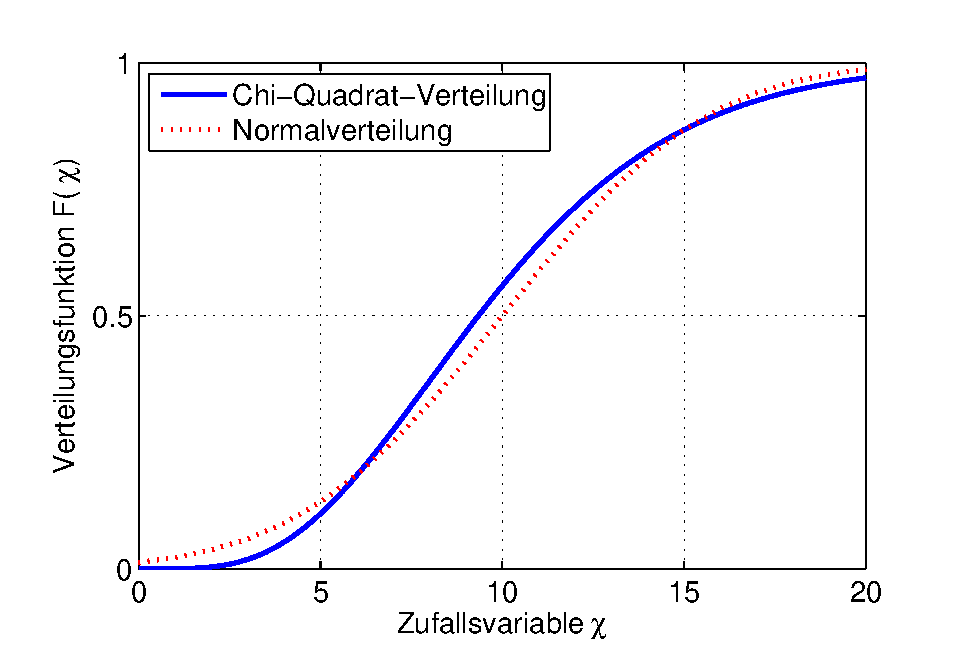
\includegraphics[width=0.5\textwidth]{Kapitel4/Bilder/image43}}
  \caption{Darstellung der Chi-Quadrat-Verteilung f\"{u}r unterschiedliche Freiheitsgrade $\nu$}
  \label{fig:Testverteilungen_ChiQuadrat1}
\end{figure}

\noindent Auch die Chi-Quadrat-Funktion l\"{a}sst sich durch die Normalverteilung ann\"{a}hern. Die Zufallsvariable $\chi$ ist asymptotisch normalverteilt mit dem Mittelwert $\mu$ aus Gleichung \eqref{eq:fourtwohundredthirtyfour} und der Varianz $\sigma^{2}$ aus Gleichung \eqref{eq:fourtwohundredthirtyfive}. Bild \ref{fig:Testverteilungen_ChiQuadrat2} vergleicht grafisch die Chi-Quadrat-Verteilung mit der Normalverteilung.

\begin{figure}[H]
  \centerline{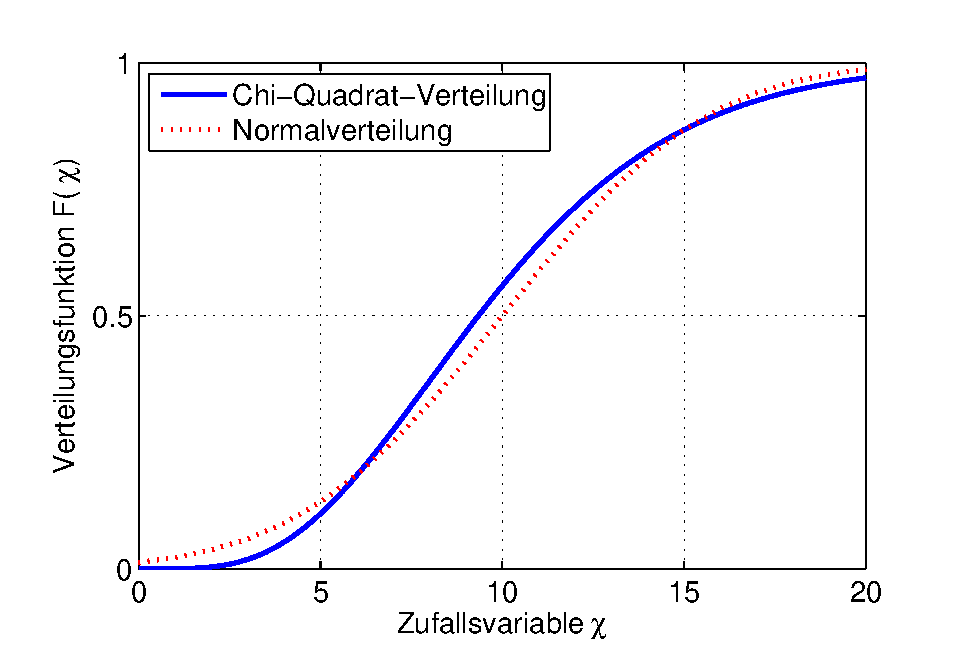
\includegraphics[width=0.5\textwidth]{Kapitel4/Bilder/image43}}
  \caption{N\"{a}herung der Chi-Quadrat-Verteilung mit N = 10 durch eine Normalverteilung mit $\mu$ = 10 und $\sigma^{2}$ = 20}
  \label{fig:Testverteilungen_ChiQuadrat2}
\end{figure}

\clearpage 

\noindent Es kann gezeigt werden, dass die Varianz einer Stichprobe von N Werten 

\begin{equation}\label{eq:fourtwohundredthirtysix}
s^{2} =\dfrac{1}{N-1} \cdot \sum _{n=1}^{N}\left(x_{n} -\bar{x}\right)^{2}
\end{equation}

\noindent aus einer normalverteilten Grundgesamtheit mit einem Mittelwert $\mu$ und einer Varianz $\sigma^{2}$ eine Chi-Quadrat-Verteilung mit $\nuup$ = N - 1 Freiheitsgraden besitzt, wenn sie vorher mit dem Faktor $\nuup$ multipliziert und durch die Varianz $\sigma^{2}$ dividiert wurde.

\begin{equation}\label{eq:fourtwohundredthirtyseven}
\chi =(N-1)\cdot \dfrac{s^{2} }{\sigma ^{2}} =\nu \cdot \dfrac{s^{2}}{\sigma ^{2}}
\end{equation}

\noindent Anwendung findet die Chi-Quadrat-Verteilung bei statistischen Aussagen zu der Varianz einer Grundgesamtheit, die aus einer Stichprobe bestimmt wird. Das ist zum Beispiel bei der Berechnung von Vertrauensintervallen f\"{u}r Varianzen und bei Hypothesentests zu Varianzen der Fall.


\subsubsection{t-Verteilung von Student}

\noindent Die Student t-Verteilung ist eine Wahrscheinlichkeitsverteilung, die von William Sealey Gosset entwickelt wurde. Er hatte festgestellt, dass der standardisierte Mittelwert normalverteilter Daten nicht mehr normalverteilt ist, wenn die Varianz des Merkmals unbekannt ist und mit der Stichprobenvarianz gesch\"{a}tzt werden muss. Die Herleitung wurde erstmals 1908 ver\"{o}ffentlicht, w\"{a}hrend Gosset in einer Guinness-Brauerei arbeitete. Da sein Arbeitgeber die Ver\"{o}ffentlichung nicht gestattete, ver\"{o}ffentlichte Gosset sie unter dem Pseudonym Student. Die zugeh\"{o}rige Theorie wurde erst durch die Arbeiten von R. A. Fisher belegt, der die Verteilung Students distribution (Students Verteilung) nannte.\newline

\noindent Zur Erkl\"{a}rung des Hintergrundes dieser Verteilung wird die eingangs diskutierte Stichprobe von N Werten x$_{1}$, x$_{2}$, {\dots}, x$_{N}$ angenommen. Die Werte stammen aus einer Grundgesamtheit mit Standard-Normalverteilung, die einen Mittelwert von $\mu$ = 0 und eine unbekannte Standardabweichung $\sigma$ besitzt. Aus der zuf\"{a}llig ausgew\"{a}hlten Stichprobe ergibt sich der Stichproben-Mittelwert 

\begin{equation}\label{eq:fourtwohundredthirtyeight}
\bar{x}=\dfrac{1}{N} \cdot \sum _{n=1}^{N}x_{n}
\end{equation}

\noindent und die Stichproben-Standardabweichung

\begin{equation}\label{eq:fourtwohundredthirtynine}
s=\sqrt{\dfrac{1}{N-1} \cdot \sum _{n=1}^{N}\left(x_{n} -\bar{x}\right)^{2}} 
\end{equation}

\noindent Gosset hat gezeigt, dass der Quotient 

\begin{equation}\label{eq:fourtwohundredfourty}
t=\dfrac{z}{\sqrt{\dfrac{\chi }{(N-1)}}} 
\end{equation}

\noindent einer standardnormalverteilten Gr\"{o}{\ss}e z und einer Gr\"{o}{\ss}e $\chi$ mit Chi-Quadrat-Verteilung eine t-Verteilung mit $\nuup$ = N - 1 Freiheitsgraden aufweist. Damit weist zum Beispiel die Gr\"{o}{\ss}e

\begin{equation}\label{eq:fourtwohundredfourtyone}
t=\dfrac{\dfrac{x-\mu }{\sigma } }{\sqrt{\dfrac{1}{(N-1)} \cdot (N-1)\cdot \dfrac{s^{2} }{\sigma ^{2}}}} =\dfrac{\dfrac{x-\mu }{\sigma} }{\sqrt{\dfrac{s^{2} }{\sigma ^{2}}}} =\dfrac{\dfrac{x-\mu }{\sigma}}{\dfrac{s}{\sigma } } =\dfrac{x-\mu}{s}
\end{equation}

\noindent eine t-Verteilung mit $\nuup$ = N - 1 Freiheitsgraden auf. Die t-Verteilung hat die Wahrscheinlichkeitsdichte f(t) von 

\begin{equation}\label{eq:fourtwohundredfourtytwo}
f(t)=\dfrac{\Gamma \left(\dfrac{\nu +1}{2} \right)}{\sqrt{\nu \cdot \pi} \cdot \Gamma \left(\dfrac{\nu}{2} \right)\cdot \left(1+\dfrac{t^{2} }{\nu} \right)^{\dfrac{\nu +1}{2}}}
\end{equation}

\noindent und die Verteilungsfunktion F(t) 

\begin{equation}\label{eq:fourtwohundredfourtythree}
F(t)=\dfrac{\Gamma \left(\dfrac{\nu +1}{2} \right)}{\sqrt{\nu \cdot \pi} \cdot \Gamma \left(\dfrac{\nu}{2} \right)} \cdot \int\limits _{-\infty }^{t}\dfrac{1}{\left(1+\dfrac{\tau ^{2} }{\nu} \right)^{\dfrac{\nu +1}{2}}} d\tau
\end{equation}


\noindent Dabei ist der Ausdruck $\Gamma$($\alpha$) die in Kapitel 4.6.3 eingef\"{u}hrte Gamma-Funktion. Aus Gleichung \eqref{eq:fourtwohundredfourtytwo} und Gleichung \eqref{eq:fourtwohundredfourtythree} wird ersichtlich, dass die t-Verteilung nur von dem Parameter $\nuup$, der Anzahl von Freiheitsgraden abh\"{a}ngig ist. F\"{u}r $\nuup$ = 1 ergibt sich eine Verteilung, die keinen Mittelwert besitzt [Fahr06]. F\"{u}r $\nuup$ $\mathrm{>}$ 1 hat die t-Verteilung wegen der Achsensymmetrie den Mittelwert 0. F\"{u}r $\nuup$ $\leq$ 2 hat die t-Verteilung keine Varianz, f\"{u}r $\nuup$ $\mathrm{>}$ 2 ergibt sich die Varianz 

\begin{equation}\label{eq:fourtwohundredfourtyfour}
\sigma ^{2} =\dfrac{\nu }{\nu -2}
\end{equation}

\noindent Mit wachsender Anzahl an Freiheitsgraden $\nuup$ strebt die Wahrscheinlichkeitsdichte der t-Verteilung gegen die Wahrscheinlichkeitsdichte der standardisierten Normalverteilung, da gilt

\begin{equation}\label{eq:fourtwohundredfourtyfive}
{\mathop{\lim }\limits_{\nu \to \infty }} \sigma ^{2} ={\mathop{\lim }\limits_{\nu \to \infty }} \left(\dfrac{\nu }{\nu -2} \right)=1
\end{equation}

\noindent Bild \ref{fig:Testverteilungen_Student} stellt die t-Verteilung f\"{u}r $\nuup$ = 2, 5 und 25 im Vergleich zur Standard-Normalverteilung mit $\mu$ = 0 und $\sigma^{2}$ = 1 dar.

\begin{figure}[H]
  \centerline{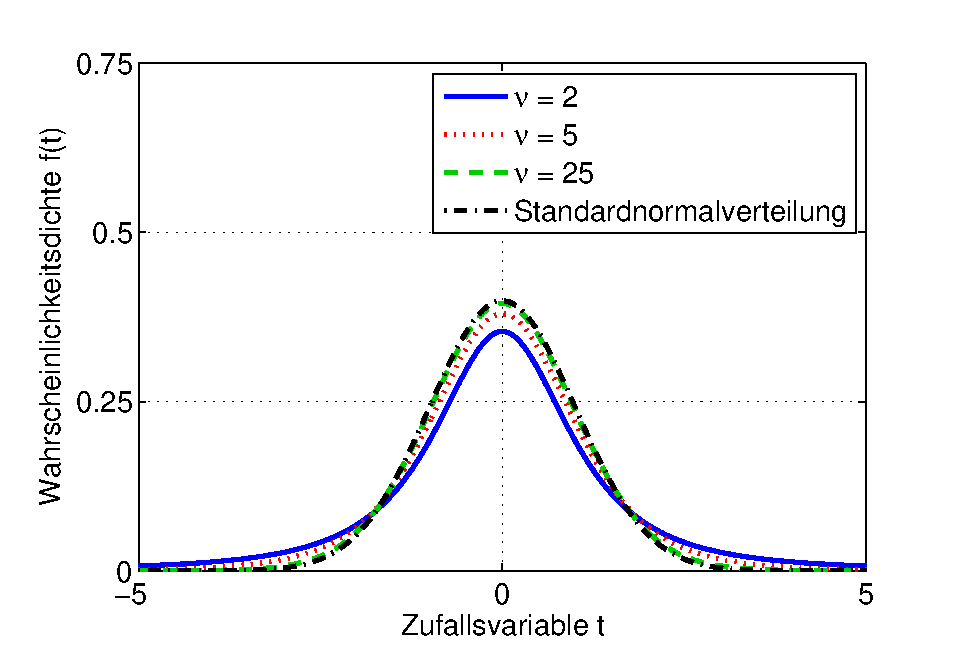
\includegraphics[width=0.5\textwidth]{Kapitel4/Bilder/image45}}
  \caption{t-Verteilung mit $\nuup$ = 2, 5 und 25 im Vergleich zur standardisierten Normalverteilung}
  \label{fig:Testverteilungen_Student}
\end{figure}

\noindent Die t-Verteilung ist breiter als die Normalverteilung mit einer Standardabweichung von $\sigma$ = s. Dieser Zusammenhang ergibt sich daraus, dass die Standardabweichung aufgrund einer Stichprobe gesch\"{a}tzt wird und damit eine gr\"{o}{\ss}ere Unsicherheit besteht als bei bekannter Standardabweichung.\newline

\noindent Die t-Verteilung wird immer verwendet, wenn der Mittelwert einer Stichprobe mit unbekannter Varianz bewertet werden soll. Zum Beispiel wird sie bei Hypothesentests dazu verwendet, um abzusch\"{a}tzen, ob ein Stichprobenwert zuf\"{a}llig von dem Mittelwert abweicht oder ob die Abweichung systematisch ist. Au{\ss}erdem wird die t-Verteilung dazu verwendet, einen Konfidenzbereich f\"{u}r einen Mittelwert einer Grundgesamtheit mit unbekannter Varianz anzugeben.

\subsubsection{f-Verteilung von Fisher}

\noindent Die f-Verteilung wurde von Ronald Aylmer Fisher entwickelt. Sie beschreibt die Verteilung einer Zufallsvariable f, die sich aus dem Quotienten zweier chi-quadrat-verteilter Zufallsvariablen ergibt, die auf ihre entsprechende Anzahl Freiheitsgrade normiert sind.

\begin{equation}\label{eq:fourtwohundredfourtysix}
f=\dfrac{\chi \left(\nu _{1} \right)/\nu _{1} }{\chi \left(\nu _{2} \right)/\nu _{2}}
\end{equation}

\noindent Die Zufallsvariable f aus Gleichung \eqref{eq:fourtwohundredfourtysix} besitzt eine f-Verteilung mit $\nuup_{1}$ und $\nuup_{2}$ Freiheitsgraden. Die Wahrscheinlichkeitsdichte der f-Verteilung ist definiert zu

\begin{equation}\label{eq:fourtwohundredfourtyseven}
f(f)=\dfrac{\Gamma \left(\dfrac{\nu _{1} +\nu _{2} }{2} \right)}{\Gamma \left(\dfrac{\nu _{1} }{2} \right)\cdot \Gamma \left(\dfrac{\nu _{2} }{2} \right)} \cdot \left(\dfrac{\nu _{1} }{\nu _{2} } \right)^{\dfrac{\nu _{1} }{2}} \cdot \dfrac{f^{\dfrac{\nu _{1} }{2} -1}}{\left(\dfrac{\nu _{1} \cdot f}{\nu _{2}} +1\right)^{\dfrac{\nu _{1} +\nu _{2}}{2}}}
\end{equation}

\noindent Die Verteilungsfunktion F(f) kann nicht analytisch berechnet werden, sondern muss numerisch bestimmt werden. F\"{u}r $\nuup_{2}$ $\mathrm{\le}$ 2 besitzt die Verteilung keinen Mittelwert. F\"{u}r $\nuup_{2}$ $\mathrm{>}$ 2 hat die f-Verteilung den Mittelwert

\begin{equation}\label{eq:fourtwohundredfourtyeight}
\mu =\dfrac{\nu _{2} }{\nu _{2} -2}
\end{equation}

\noindent F\"{u}r $\nuup_{2}$ $\leq$ 4 hat die f-Verteilung keine Varianz, f\"{u}r $\nuup_{2}$ $\mathrm{>}$ 4 ergibt sich die Varianz zu

\begin{equation}\label{eq:fourtwohundredfourtynine}
\sigma ^{2} =\dfrac{2\cdot \nu _{2}^{2} \cdot \left(\nu _{2} +\nu _{1} -2\right)}{\nu _{1} \cdot \left(\nu _{2} -4\right)\cdot \left(\nu _{2} -2\right)^{2} }
\end{equation}

\noindent Bild \ref{fig:Testverteilungen_Fisher} stellt die Wahrscheinlichkeitsdichte f(f) und die Verteilungsfunktion F(f) der f-Verteilung f\"{u}r Wertekombinationen ($\nuup_{1}$, $\nuup_{2}$) = (4, 4), (4, 20), (20, 4) und (20, 20) dar.

\begin{figure}[H]
  \centerline{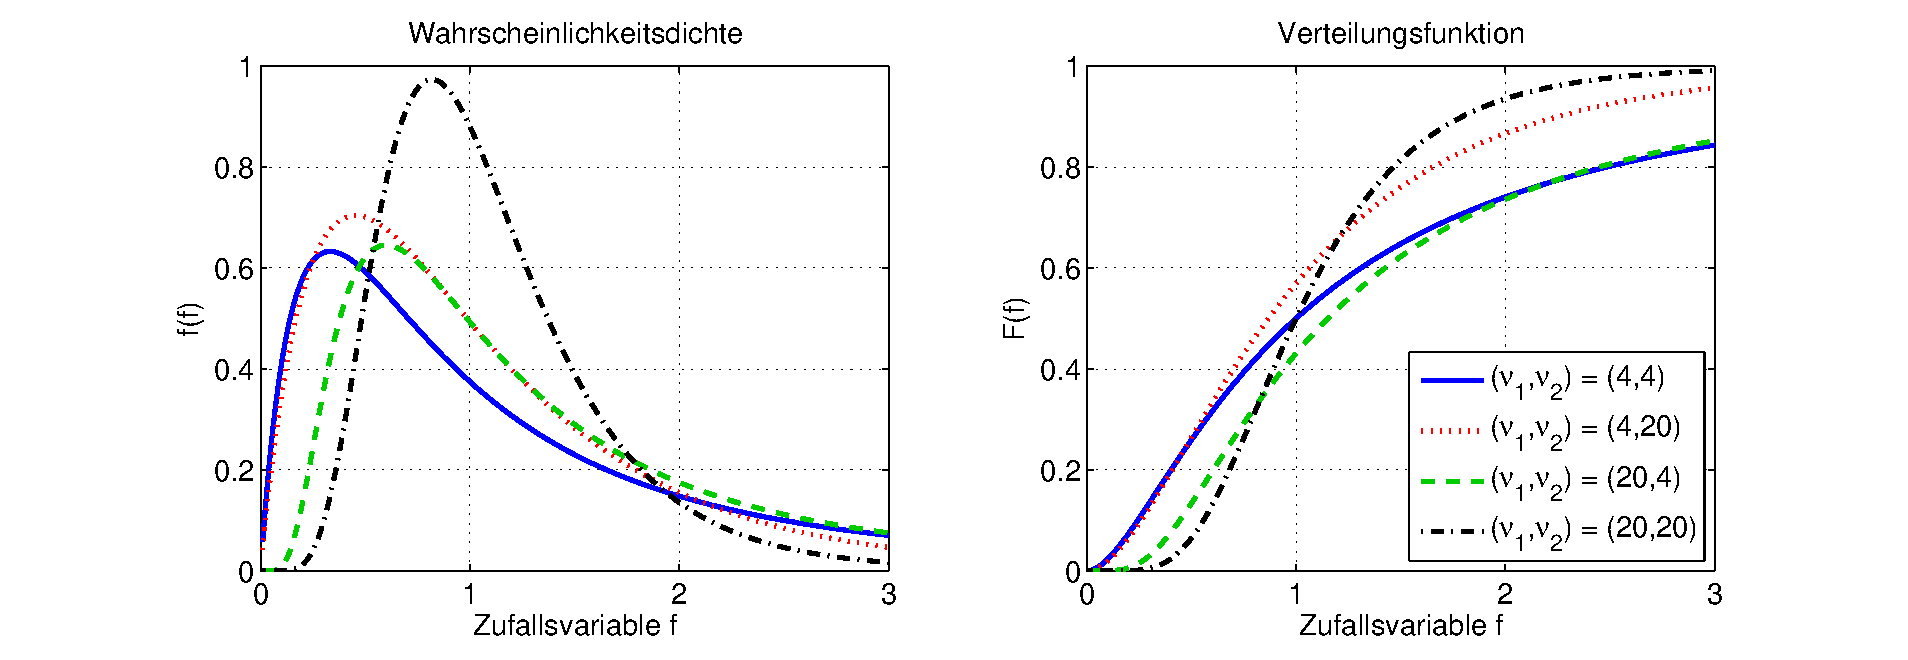
\includegraphics[width=1\textwidth]{Kapitel4/Bilder/image46}}
  \caption{F-Verteilung f\"{u}r Wertekombinationen ($\nuup_{1}$, $\nuup_{2}$) = (4, 4), (4, 20), (20, 4) und (20, 20)}
  \label{fig:Testverteilungen_Fisher}
\end{figure}

\noindent Dieser theoretischen Definition der f-Verteilung liegt die Aufgabe zugrunde, eine Verteilungsfunktion f\"{u}r das Verh\"{a}ltnis von zwei Varianzen auf Basis von zwei Stichproben abzusch\"{a}tzen. Ausgangspunkt sind zwei Stichproben x$_{1}$, x$_{2}$, {\dots}, x$_{N}$ und y$_{1}$, y$_{2}$, {\dots}, y${}_{M}$. Die Stichproben stammen aus unterschiedlichen normalverteilten Grundgesamtheiten, die die Varianz $\sigma_{X}^{2}$ beziehungsweise $\sigma_{Y}^{2}$ besitzen. 

\noindent Mit den Erkenntnissen aus Gleichung \eqref{eq:fourtwohundredfourtyseven} zur Beschreibung einer chi-quadrat-verteilten Gr\"{o}{\ss}e und der allgemeinen Definition einer f-verteilten Zufallsvariablen f aus Gleichung \eqref{eq:fourtwohundredfourtysix} ergibt das Verh\"{a}ltnis der empirischen Varianzen

\begin{equation}\label{eq:fourtwohundredfifty}
f=\dfrac{\chi \left(\nu _{1} \right)/\nu _{1} }{\chi \left(\nu _{2} \right)/\nu _{2} } =\dfrac{\dfrac{\nu _{X} \cdot s_{X}^{2} }{\sigma _{X}^{2} } \cdot \dfrac{1}{\nu _{X} } }{\dfrac{\nu _{Y} \cdot s_{Y}^{2} }{\sigma _{Y}^{2} } \cdot \dfrac{1}{\nu _{Y} } } =\dfrac{s_{X}^{2} }{s_{Y}^{2} } \cdot \dfrac{\sigma _{Y}^{2} }{\sigma _{X}^{2} }
\end{equation}

\noindent eine f-Verteilung mit den Freiheitsgraden $\nuup_{1}$ und $\nuup_{2}$.\newline

\noindent Die f-Verteilung kann daher zum Beispiel bei der Varianzanalyse verwendet werden, um festzustellen, ob die Grundgesamtheiten zweier Stichproben die gleiche Varianz haben. Dar\"{u}ber hinaus wird sie bei Regressions- und Varianzanalysen eingesetzt, um zu testen, ob die jeweiligen Einflussgr\"{o}{\ss}en signifikant sind oder nicht. 


\subsubsection{Zusammenfassung der Pr\"{u}f- oder Testverteilungen}

\noindent Die t-Verteilung und die Chi-Quadrat-Verteilung leiten sich aus der Normalverteilung ab, die f-Verteilung kann durch die Logarithmische Normalverteilung angen\"{a}hert werden. Diese Zusammenh\"{a}nge sind in Bild \ref{fig:UebersichtTestverteilungen} grafisch dargestellt.\newline

\noindent Es wird sich zeigen, dass diese Verteilungen f\"{u}r das L\"{o}sen von Aufgabenstellungen anwenden lassen, bei den Parameter gesch\"{a}tzt werden und eine Aussage \"{u}ber die Genauigkeit der Sch\"{a}tzung gemacht werden soll. Das dabei verwendete Grundprinzip ist immer dasselbe. Auf Basis einer Stichprobe wird ein Parameter einer Verteilung gesch\"{a}tzt. Da es sich um eine zuf\"{a}llige Stichprobe handelt, ist auch der gesch\"{a}tzte Parameter eine Zufallsgr\"{o}{\ss}e. Mithilfe der Testverteilungen wird die Sicherheit bewertet, mit der der Parameter bestimmt wurde. Ihre Wahrscheinlichkeitsdichten, Mittelwerte und Standardabweichungen sowie ihre Anwendungsbereiche sind in Tabelle \ref{tab:foureightteen} wiedergegeben.

\noindent 
\begin{figure}[H]
  \centerline{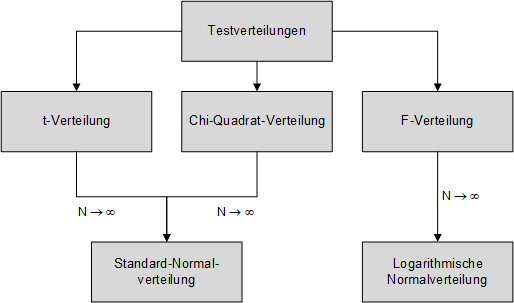
\includegraphics[width=0.8\textwidth]{Kapitel4/Bilder/image47}}
  \caption{Zusammenhang der eingef\"{u}hrten Testverteilungen}
  \label{fig:UebersichtTestverteilungen}
\end{figure}

\clearpage

\begin{table}[H]
\setlength{\arrayrulewidth}{.1em}
\caption{\"{U}bersicht \"{u}ber die Testverteilungen und ihre Anwendungen}
\setlength{\fboxsep}{0pt}%
\colorbox{lightgray}{%
\arrayrulecolor{white}%
\begin{tabular}{| c | c | c |}
\hline
\parbox[c][0.3in][c]{1.9in}{\smallskip\centering\textbf{\fontfamily{phv}\selectfont{Name und Anwendung}}} &
\parbox[c][0.3in][c]{2.6in}{\smallskip\centering\textbf{\fontfamily{phv}\selectfont{Wahrscheinlichkeitsverteilung}}} &
\parbox[c][0.3in][c]{1.9in}{\smallskip\centering\textbf{\fontfamily{phv}\selectfont{Kenngr\"{o}{\ss}en $\mu$ und $\sigma ^{2}$}}}\\ \hline

\parbox[c][1.4in][c]{1.9in}{\centering\fontfamily{phv}\selectfont{t-Verteilung mit $\nu$ Freiheitsgraden \newline
\\
Statistische Bewertung von Mittelwerten auf Basis von Stichproben bei unbekannter Varianz}} & 
\parbox[c][1.4in][c]{2.6in}{\centering\fontfamily{phv}\selectfont{$f(t)=\dfrac{\Gamma \left(\dfrac{\nu +1}{2} \right)}{\sqrt{\nu \cdot \pi} \cdot \Gamma \left(\dfrac{\nu }{2} \right)\cdot \left(1+\dfrac{t^{2} }{\nu} \right)^{\dfrac{\nu +1}{2} } } $}} &
\parbox[c][1.4in][c]{1.9in}{\centering\fontfamily{phv}\selectfont{$\mu =0$\bigskip

$\sigma ^{2} =\dfrac{\nu }{\nu -2} $}}\\
\hline

\parbox[c][1.6in][c]{1.9in}{\centering\fontfamily{phv}\selectfont{Chi$^{2}$-Verteilung mit $\nu$ Freiheitsgraden\newline
\\
Statistische Bewertung der Varianz einer Grundgesamtheitauf Basis von Stichproben}} & 
\parbox[c][1.6in][c]{2.6in}{\centering\fontfamily{phv}\selectfont{$f\left(\chi \right)=K_{\nu} \cdot \chi ^{\dfrac{\nu -2}{2}} \cdot e^{-\dfrac{\chi}{2}} $}} &
\parbox[c][1.6in][c]{1.9in}{\centering\fontfamily{phv}\selectfont{$\mu =\nu$\bigskip

$\sigma ^{2} =2\cdot \nu $}}\\
\hline

\parbox[c][1.6in][c]{1.9in}{\centering\fontfamily{phv}\selectfont{f-Verteilung mit $\nuup_{1}$, $\nuup_{2}$ Freiheitsgraden\newline
\\
Statistische Vergleich der Varianz zweier Grundgesamtheitenauf Basis von Stichproben}} & 
\parbox[c][1.6in][c]{2.6in}{\centering\fontfamily{phv}\selectfont{$f\left(f\right)=\dfrac{\Gamma \left(\dfrac{\nu _{1} +\nu _{2} }{2} \right)}{\Gamma \left(\dfrac{\nu _{1} }{2} \right)\cdot \Gamma \left(\dfrac{\nu _{2} }{2} \right)} \cdot \left(\dfrac{\nu _{1} }{\nu _{2} } \right)^{\dfrac{\nu _{1} }{2} } \cdot \dfrac{f^{\dfrac{\nu _{1} }{2} -1} }{\left(\dfrac{\nu _{1} \cdot f}{\nu _{2}} +1\right)^{\dfrac{\nu _{1} +\nu _{2}}{2}}} $}} &
\parbox[c][1.6in][c]{1.9in}{\centering\fontfamily{phv}\selectfont{$\mu =\dfrac{\nu _{2} }{\nu _{2} -2} $\bigskip

$\sigma ^{2} =\dfrac{2\cdot \nu _{2}^{2} \cdot \left(\nu _{2} +\nu _{1} -2\right)}{\nu _{1} \cdot \left(\nu _{2} -4\right)\cdot \left(\nu _{2} -2\right)^{2} } $}}\\
\hline

\end{tabular}%
}
\label{tab:foureightteen}
\end{table}

\clearpage

\noindent In der Statistic-Toolbox von MATLAB sind die Pr\"{u}f- und Testverteilungen implementiert. Tabelle \ref{tab:fournineteen} gibt einen \"{U}berblick \"{u}ber die entsprechenden Funktionen.

\begin{table}[H]
\caption{\"{U}bersicht \"{u}ber die Testverteilungen in MATLAB}
\setlength{\fboxsep}{0pt}%
\colorbox{lightgray}{%
\arrayrulecolor{white}%
\begin{tabular}{| c | c | c | c |}
\hline
\parbox[c][0.7in][c]{1.1in}{\smallskip\centering\textbf{\fontfamily{phv}\selectfont{Verteilung}}} & 
\parbox[c][0.7in][c]{1.7in}{\smallskip\centering\textbf{\fontfamily{phv}\selectfont{Dichtefunktion f(x)}}} &
\parbox[c][0.7in][c]{1.7in}{\smallskip\centering\textbf{\fontfamily{phv}\selectfont{Wahrscheinlichkeits-funktion F(x)}}} &
\parbox[c][0.7in][c]{1.7in}{\smallskip\centering\textbf{\fontfamily{phv}\selectfont{inverse Wahrscheinlichkeitsfunktion F-1(x)}}}\\ \hline

\parbox[c][0.3in][c]{1.1in}{\centering\fontfamily{phv}\selectfont{t-Verteilung}} &
\parbox[c][0.3in][c]{1.7in}{\centering\fontfamily{phv}\selectfont{tpdf(x,$\nu$)}} &
\parbox[c][0.3in][c]{1.7in}{\centering\fontfamily{phv}\selectfont{tcdf(x,$\nu$)}} &
\parbox[c][0.3in][c]{1.7in}{\centering\fontfamily{phv}\selectfont{tinv(P,$\nu$)}} \\ \hline

\parbox[c][0.5in][c]{1.1in}{\centering\fontfamily{phv}\selectfont{Chi-Quadrat-Verteilung}} &
\parbox[c][0.5in][c]{1.7in}{\centering\fontfamily{phv}\selectfont{chi2pdf(x,$\nu$)}} &
\parbox[c][0.5in][c]{1.7in}{\centering\fontfamily{phv}\selectfont{chi2cdf(x,$\nu$}} &
\parbox[c][0.5in][c]{1.7in}{\centering\fontfamily{phv}\selectfont{chi2inv(P,$\nu$}} \\ \hline

\parbox[c][0.3in][c]{1.1in}{\centering\fontfamily{phv}\selectfont{f-Verteilung}} &
\parbox[c][0.3in][c]{1.7in}{\centering\fontfamily{phv}\selectfont{fpdf(x,$\nu$ 1,$\nu$ 2)}} &
\parbox[c][0.3in][c]{1.7in}{\centering\fontfamily{phv}\selectfont{fcdf(x,$\nu$ 1,$\nu$ 2)}} &
\parbox[c][0.3in][c]{1.7in}{\centering\fontfamily{phv}\selectfont{finv(P,$\nu$ 1,$\nu$ 2)}} \\ \hline

\end{tabular}%
}\bigskip
\label{tab:fournineteen}
\end{table}

\noindent Auch in Python sind entsprechende Funktionen implementiert, Tabelle \ref{tab:fourtwenty} gibt einen \"{U}berblick \"{u}ber diese Funktionen.

\begin{table}[H]
\caption{\"{U}bersicht \"{u}ber die Testverteilungen in der Python Bibliothek scipy.stats}
\setlength{\fboxsep}{0pt}%
\colorbox{lightgray}{%
\arrayrulecolor{white}%
\begin{tabular}{| c | c | c | c |}
\hline
\parbox[c][0.7in][c]{1.1in}{\smallskip\centering\textbf{\fontfamily{phv}\selectfont{Verteilung}}} & 
\parbox[c][0.7in][c]{1.7in}{\smallskip\centering\textbf{\fontfamily{phv}\selectfont{Dichtefunktion f(x)}}} &
\parbox[c][0.7in][c]{1.7in}{\smallskip\centering\textbf{\fontfamily{phv}\selectfont{Wahrscheinlichkeits-funktion F(x)}}} &
\parbox[c][0.7in][c]{1.7in}{\smallskip\centering\textbf{\fontfamily{phv}\selectfont{inverse Wahrscheinlichkeitsfunktion F-1(x)}}}\\ \hline

\parbox[c][0.3in][c]{1.1in}{\centering\fontfamily{phv}\selectfont{t-Verteilung}} &
\parbox[c][0.3in][c]{1.7in}{\centering\fontfamily{phv}\selectfont{t.pdf(x,$\nu$)}} &
\parbox[c][0.3in][c]{1.7in}{\centering\fontfamily{phv}\selectfont{t.cdf(x,$\nu$)}} &
\parbox[c][0.3in][c]{1.7in}{\centering\fontfamily{phv}\selectfont{t.ppf(P,$\nu$)}} \\ \hline

\parbox[c][0.5in][c]{1.1in}{\centering\fontfamily{phv}\selectfont{Chi-Quadrat-Verteilung}} &
\parbox[c][0.5in][c]{1.7in}{\centering\fontfamily{phv}\selectfont{chi2pdf(x,$\nu$)}} &
\parbox[c][0.5in][c]{1.7in}{\centering\fontfamily{phv}\selectfont{chi2cdf(x,$\nu$}} &
\parbox[c][0.5in][c]{1.7in}{\centering\fontfamily{phv}\selectfont{chi2inv(P,$\nu$}} \\ \hline

\parbox[c][0.3in][c]{1.1in}{\centering\fontfamily{phv}\selectfont{f-Verteilung}} &
\parbox[c][0.3in][c]{1.7in}{\centering\fontfamily{phv}\selectfont{fpdf(x,$\nu$ 1,$\nu$ 2)}} &
\parbox[c][0.3in][c]{1.7in}{\centering\fontfamily{phv}\selectfont{fcdf(x,$\nu$ 1,$\nu$ 2)}} &
\parbox[c][0.3in][c]{1.7in}{\centering\fontfamily{phv}\selectfont{finv(P,$\nu$ 1,$\nu$2)}} \\ \hline

\end{tabular}%
}\bigskip
\label{tab:fourtwenty}
\end{table}

\clearpage

\subsection{Literatur}

\begin{tabular}{|p{0.6in}|p{5.7in}|} \hline 
[Krey91] & Kreyszig, Erwin: Statistische Methoden und ihre Anwendungen\newline 4., unver\"{a}nderter Nachdruck der 7. Auflage\newline Vandenhoeck \& Ruprecht, G\"{o}ttingen, 1991 \\ \hline 
[Fahr06] & Fahrmeir, Ludwig; K\"{u}nstler, Rita; Pigeot, Iris; Tutz, Gerhard: Der Weg zur Datenanalyse\newline 6. Auflage\newline Springer Berlin Heidelberg New York, 2006 \\ \hline 
[Ross06] & Ross, M. Sheldon: Statistik f\"{u}r Ingenieure und Naturwissenschaftler\newline 3. Auflage\newline Spektrum Akademischer Verlag, M\"{u}nchen, 2006 \\ \hline 
\end{tabular}
